% Options for packages loaded elsewhere
% Options for packages loaded elsewhere
\PassOptionsToPackage{unicode}{hyperref}
\PassOptionsToPackage{hyphens}{url}
\PassOptionsToPackage{dvipsnames,svgnames,x11names}{xcolor}
%
\documentclass[
  letterpaper,
]{report}
\usepackage{xcolor}
\usepackage[margin=1in]{geometry}
\usepackage{amsmath,amssymb}
\setcounter{secnumdepth}{5}
\usepackage{iftex}
\ifPDFTeX
  \usepackage[T1]{fontenc}
  \usepackage[utf8]{inputenc}
  \usepackage{textcomp} % provide euro and other symbols
\else % if luatex or xetex
  \usepackage{unicode-math} % this also loads fontspec
  \defaultfontfeatures{Scale=MatchLowercase}
  \defaultfontfeatures[\rmfamily]{Ligatures=TeX,Scale=1}
\fi
\usepackage{lmodern}
\ifPDFTeX\else
  % xetex/luatex font selection
\fi
% Use upquote if available, for straight quotes in verbatim environments
\IfFileExists{upquote.sty}{\usepackage{upquote}}{}
\IfFileExists{microtype.sty}{% use microtype if available
  \usepackage[]{microtype}
  \UseMicrotypeSet[protrusion]{basicmath} % disable protrusion for tt fonts
}{}
\makeatletter
\@ifundefined{KOMAClassName}{% if non-KOMA class
  \IfFileExists{parskip.sty}{%
    \usepackage{parskip}
  }{% else
    \setlength{\parindent}{0pt}
    \setlength{\parskip}{6pt plus 2pt minus 1pt}}
}{% if KOMA class
  \KOMAoptions{parskip=half}}
\makeatother
% Make \paragraph and \subparagraph free-standing
\makeatletter
\ifx\paragraph\undefined\else
  \let\oldparagraph\paragraph
  \renewcommand{\paragraph}{
    \@ifstar
      \xxxParagraphStar
      \xxxParagraphNoStar
  }
  \newcommand{\xxxParagraphStar}[1]{\oldparagraph*{#1}\mbox{}}
  \newcommand{\xxxParagraphNoStar}[1]{\oldparagraph{#1}\mbox{}}
\fi
\ifx\subparagraph\undefined\else
  \let\oldsubparagraph\subparagraph
  \renewcommand{\subparagraph}{
    \@ifstar
      \xxxSubParagraphStar
      \xxxSubParagraphNoStar
  }
  \newcommand{\xxxSubParagraphStar}[1]{\oldsubparagraph*{#1}\mbox{}}
  \newcommand{\xxxSubParagraphNoStar}[1]{\oldsubparagraph{#1}\mbox{}}
\fi
\makeatother

\usepackage{color}
\usepackage{fancyvrb}
\newcommand{\VerbBar}{|}
\newcommand{\VERB}{\Verb[commandchars=\\\{\}]}
\DefineVerbatimEnvironment{Highlighting}{Verbatim}{commandchars=\\\{\}}
% Add ',fontsize=\small' for more characters per line
\usepackage{framed}
\definecolor{shadecolor}{RGB}{241,243,245}
\newenvironment{Shaded}{\begin{snugshade}}{\end{snugshade}}
\newcommand{\AlertTok}[1]{\textcolor[rgb]{0.68,0.00,0.00}{#1}}
\newcommand{\AnnotationTok}[1]{\textcolor[rgb]{0.37,0.37,0.37}{#1}}
\newcommand{\AttributeTok}[1]{\textcolor[rgb]{0.40,0.45,0.13}{#1}}
\newcommand{\BaseNTok}[1]{\textcolor[rgb]{0.68,0.00,0.00}{#1}}
\newcommand{\BuiltInTok}[1]{\textcolor[rgb]{0.00,0.23,0.31}{#1}}
\newcommand{\CharTok}[1]{\textcolor[rgb]{0.13,0.47,0.30}{#1}}
\newcommand{\CommentTok}[1]{\textcolor[rgb]{0.37,0.37,0.37}{#1}}
\newcommand{\CommentVarTok}[1]{\textcolor[rgb]{0.37,0.37,0.37}{\textit{#1}}}
\newcommand{\ConstantTok}[1]{\textcolor[rgb]{0.56,0.35,0.01}{#1}}
\newcommand{\ControlFlowTok}[1]{\textcolor[rgb]{0.00,0.23,0.31}{\textbf{#1}}}
\newcommand{\DataTypeTok}[1]{\textcolor[rgb]{0.68,0.00,0.00}{#1}}
\newcommand{\DecValTok}[1]{\textcolor[rgb]{0.68,0.00,0.00}{#1}}
\newcommand{\DocumentationTok}[1]{\textcolor[rgb]{0.37,0.37,0.37}{\textit{#1}}}
\newcommand{\ErrorTok}[1]{\textcolor[rgb]{0.68,0.00,0.00}{#1}}
\newcommand{\ExtensionTok}[1]{\textcolor[rgb]{0.00,0.23,0.31}{#1}}
\newcommand{\FloatTok}[1]{\textcolor[rgb]{0.68,0.00,0.00}{#1}}
\newcommand{\FunctionTok}[1]{\textcolor[rgb]{0.28,0.35,0.67}{#1}}
\newcommand{\ImportTok}[1]{\textcolor[rgb]{0.00,0.46,0.62}{#1}}
\newcommand{\InformationTok}[1]{\textcolor[rgb]{0.37,0.37,0.37}{#1}}
\newcommand{\KeywordTok}[1]{\textcolor[rgb]{0.00,0.23,0.31}{\textbf{#1}}}
\newcommand{\NormalTok}[1]{\textcolor[rgb]{0.00,0.23,0.31}{#1}}
\newcommand{\OperatorTok}[1]{\textcolor[rgb]{0.37,0.37,0.37}{#1}}
\newcommand{\OtherTok}[1]{\textcolor[rgb]{0.00,0.23,0.31}{#1}}
\newcommand{\PreprocessorTok}[1]{\textcolor[rgb]{0.68,0.00,0.00}{#1}}
\newcommand{\RegionMarkerTok}[1]{\textcolor[rgb]{0.00,0.23,0.31}{#1}}
\newcommand{\SpecialCharTok}[1]{\textcolor[rgb]{0.37,0.37,0.37}{#1}}
\newcommand{\SpecialStringTok}[1]{\textcolor[rgb]{0.13,0.47,0.30}{#1}}
\newcommand{\StringTok}[1]{\textcolor[rgb]{0.13,0.47,0.30}{#1}}
\newcommand{\VariableTok}[1]{\textcolor[rgb]{0.07,0.07,0.07}{#1}}
\newcommand{\VerbatimStringTok}[1]{\textcolor[rgb]{0.13,0.47,0.30}{#1}}
\newcommand{\WarningTok}[1]{\textcolor[rgb]{0.37,0.37,0.37}{\textit{#1}}}

\usepackage{longtable,booktabs,array}
\usepackage{calc} % for calculating minipage widths
% Correct order of tables after \paragraph or \subparagraph
\usepackage{etoolbox}
\makeatletter
\patchcmd\longtable{\par}{\if@noskipsec\mbox{}\fi\par}{}{}
\makeatother
% Allow footnotes in longtable head/foot
\IfFileExists{footnotehyper.sty}{\usepackage{footnotehyper}}{\usepackage{footnote}}
\makesavenoteenv{longtable}
\usepackage{graphicx}
\makeatletter
\newsavebox\pandoc@box
\newcommand*\pandocbounded[1]{% scales image to fit in text height/width
  \sbox\pandoc@box{#1}%
  \Gscale@div\@tempa{\textheight}{\dimexpr\ht\pandoc@box+\dp\pandoc@box\relax}%
  \Gscale@div\@tempb{\linewidth}{\wd\pandoc@box}%
  \ifdim\@tempb\p@<\@tempa\p@\let\@tempa\@tempb\fi% select the smaller of both
  \ifdim\@tempa\p@<\p@\scalebox{\@tempa}{\usebox\pandoc@box}%
  \else\usebox{\pandoc@box}%
  \fi%
}
% Set default figure placement to htbp
\def\fps@figure{htbp}
\makeatother


% definitions for citeproc citations
\NewDocumentCommand\citeproctext{}{}
\NewDocumentCommand\citeproc{mm}{%
  \begingroup\def\citeproctext{#2}\cite{#1}\endgroup}
\makeatletter
 % allow citations to break across lines
 \let\@cite@ofmt\@firstofone
 % avoid brackets around text for \cite:
 \def\@biblabel#1{}
 \def\@cite#1#2{{#1\if@tempswa , #2\fi}}
\makeatother
\newlength{\cslhangindent}
\setlength{\cslhangindent}{1.5em}
\newlength{\csllabelwidth}
\setlength{\csllabelwidth}{3em}
\newenvironment{CSLReferences}[2] % #1 hanging-indent, #2 entry-spacing
 {\begin{list}{}{%
  \setlength{\itemindent}{0pt}
  \setlength{\leftmargin}{0pt}
  \setlength{\parsep}{0pt}
  % turn on hanging indent if param 1 is 1
  \ifodd #1
   \setlength{\leftmargin}{\cslhangindent}
   \setlength{\itemindent}{-1\cslhangindent}
  \fi
  % set entry spacing
  \setlength{\itemsep}{#2\baselineskip}}}
 {\end{list}}
\usepackage{calc}
\newcommand{\CSLBlock}[1]{\hfill\break\parbox[t]{\linewidth}{\strut\ignorespaces#1\strut}}
\newcommand{\CSLLeftMargin}[1]{\parbox[t]{\csllabelwidth}{\strut#1\strut}}
\newcommand{\CSLRightInline}[1]{\parbox[t]{\linewidth - \csllabelwidth}{\strut#1\strut}}
\newcommand{\CSLIndent}[1]{\hspace{\cslhangindent}#1}



\setlength{\emergencystretch}{3em} % prevent overfull lines

\providecommand{\tightlist}{%
  \setlength{\itemsep}{0pt}\setlength{\parskip}{0pt}}



 


\makeatletter
\@ifpackageloaded{tcolorbox}{}{\usepackage[skins,breakable]{tcolorbox}}
\@ifpackageloaded{fontawesome5}{}{\usepackage{fontawesome5}}
\definecolor{quarto-callout-color}{HTML}{909090}
\definecolor{quarto-callout-note-color}{HTML}{0758E5}
\definecolor{quarto-callout-important-color}{HTML}{CC1914}
\definecolor{quarto-callout-warning-color}{HTML}{EB9113}
\definecolor{quarto-callout-tip-color}{HTML}{00A047}
\definecolor{quarto-callout-caution-color}{HTML}{FC5300}
\definecolor{quarto-callout-color-frame}{HTML}{acacac}
\definecolor{quarto-callout-note-color-frame}{HTML}{4582ec}
\definecolor{quarto-callout-important-color-frame}{HTML}{d9534f}
\definecolor{quarto-callout-warning-color-frame}{HTML}{f0ad4e}
\definecolor{quarto-callout-tip-color-frame}{HTML}{02b875}
\definecolor{quarto-callout-caution-color-frame}{HTML}{fd7e14}
\makeatother
\makeatletter
\@ifpackageloaded{caption}{}{\usepackage{caption}}
\AtBeginDocument{%
\ifdefined\contentsname
  \renewcommand*\contentsname{Table of contents}
\else
  \newcommand\contentsname{Table of contents}
\fi
\ifdefined\listfigurename
  \renewcommand*\listfigurename{List of Figures}
\else
  \newcommand\listfigurename{List of Figures}
\fi
\ifdefined\listtablename
  \renewcommand*\listtablename{List of Tables}
\else
  \newcommand\listtablename{List of Tables}
\fi
\ifdefined\figurename
  \renewcommand*\figurename{Figure}
\else
  \newcommand\figurename{Figure}
\fi
\ifdefined\tablename
  \renewcommand*\tablename{Table}
\else
  \newcommand\tablename{Table}
\fi
}
\@ifpackageloaded{float}{}{\usepackage{float}}
\floatstyle{ruled}
\@ifundefined{c@chapter}{\newfloat{codelisting}{h}{lop}}{\newfloat{codelisting}{h}{lop}[chapter]}
\floatname{codelisting}{Listing}
\newcommand*\listoflistings{\listof{codelisting}{List of Listings}}
\makeatother
\makeatletter
\makeatother
\makeatletter
\@ifpackageloaded{caption}{}{\usepackage{caption}}
\@ifpackageloaded{subcaption}{}{\usepackage{subcaption}}
\makeatother
\usepackage{bookmark}
\IfFileExists{xurl.sty}{\usepackage{xurl}}{} % add URL line breaks if available
\urlstyle{same}
\hypersetup{
  pdftitle={Proximal-to-Distal Energy Transfer in the Golf Swing},
  pdfauthor={Dieter Olson},
  pdfkeywords={golf swing, proximal-to-distal sequencing, kinematic
sequence, energy transfer, counterfactual dynamics, ZTCF, ZVCF, double
pendulum, two-hand wrench, shaft flexibility, moving-base
dynamics, work-energy accounting, multibody constraints, wrench
transport, ground reaction force, contact dynamics, force
plate, reference-frame invariance, muscle redundancy, activation
dynamics, cross-engine pose interchange, task robustness, motor
abundance, perturbation response, Pareto control},
  colorlinks=true,
  linkcolor={blue},
  filecolor={Maroon},
  citecolor={Blue},
  urlcolor={Blue},
  pdfcreator={LaTeX via pandoc}}


\title{Proximal-to-Distal Energy Transfer in the Golf Swing}
\usepackage{etoolbox}
\makeatletter
\providecommand{\subtitle}[1]{% add subtitle to \maketitle
  \apptocmd{\@title}{\par {\large #1 \par}}{}{}
}
\makeatother
\subtitle{Mechanisms, Evidence, and Counterfactual Tests of
Distal-Handoff Timing}
\author{Dieter Olson}
\date{2026-08-08}
\begin{document}
\maketitle
\begin{abstract}
Proximal-to-distal (P→D) sequencing --- the ordered peaking of pelvis,
thorax, arm, and club rotational speeds --- is the most widely reported
organizing principle of the golf downswing, and it is usually read as
evidence that mechanical energy should be passed outward along the
kinetic chain as early and as completely as possible. This study reviews
the mechanics and the empirical literature behind that reading and asks
the sharper question: \emph{when} during the downswing should the P→D
transfer occur? Double-pendulum mechanics, delayed-release simulation,
optimal control, and the segmental kinetic-energy literature motivate a
model hypothesis in which distal actuation is delayed while proximal
speed develops and the distal handoff accelerates later. We formalize
this delayed-actuation hypothesis in the language of zero-torque
counterfactual (ZTCF) and zero-velocity counterfactual (ZVCF)
decompositions, and test it in a reproducible two-segment golf model
using an exact interaction-force decomposition, a matched-state
torque-killswitch comparison, a wrist-torque timing sweep (92 torque
programs), pointwise drift/control counterfactual decompositions, and
Robertson-Winter style wrist-interface power accounting, all generated
by committed, reproducible scripts. In this model, driving the wrist
from the top produced 15.3\% and 10.7\% less clubhead speed than the
corresponding passive-wrist programs at the two tested shoulder-torque
levels, while delaying the wrist drive to the grid-selected onset
produced 12.4\% and 7.8\% more. Of the 92 idealized commands tested, a
restrain-then-drive program produced the highest speed at both
shoulder-torque levels. The energy accounting shows that the selected
programs move \emph{less} energy into the club early and far more late,
with negative early work by the modeled wrist actuator. That sign
describes the imposed control law; it does not identify muscle action or
human intent. We interpret these results against the literature and
state their limitations: the primary timing estimand uses a planar 2-DOF
model with a fixed hub and rigid shaft, while the later model tiers
answer narrower moving-base, flexible/modal-shaft, spatial, and contact
questions without supplying subject-calibrated human validation. A
one-at-a-time sensitivity study spanning 13 parameter cases preserves
the strategy ordering but shifts the selected onset. First-order command
transitions from 20 to 50 ms also preserve the registered ordering while
moving the selected program. Neither sweep is a continuous
optimal-control solution or a human timing prescription. The force
analysis resolves the geometric sine and cosine projections that
determine whether distal centripetal and tangential forces transfer
power. A separate audit of the author's prior two-hand WSCG model
reconstructs all 2,801 stored samples and shows that a -19.63 N m
pointwise zero-command midpoint couple is generated entirely by
separated contact forces. It also distinguishes couple sign from power
sign and verifies the predicted linear grip-separation and
relative-orientation geometry. A matched rigid/flexible three-coordinate
surrogate then separates control, momentum, gravity, joint damping,
shaft elasticity, and shaft damping with closed work--energy accounting.
In its reference case, flex changes delivery speed by +0.108 m/s, while
gravity and joint-damping ablations are substantially larger; broad
stiffness, damping, torque-cut, endpoint-window, and timestep sweeps
bound the result. A forward constrained two-arm model then branches an
exact same-state zero-command trajectory at 0.200 s. Its contact-force
couple remains negative for the full 50 ms branch and reaches -7.43 N m;
removing both grip moment arms collapses that couple exactly to zero,
while timestep and projection studies bound the numerical result. A
coupled extension then admits a finite-mass translating base, two
constrained arms, and a two-segment compliant club in one forward KKT
system. Base motion and shaft flex are endogenous; a same-state
zero-command branch retains a negative force-generated couple for 50 ms,
the coincident-grip control removes it exactly, and work--energy and
contact-power identities close under timestep refinement. These are
planar model-feasibility results, not physiological or human evidence. A
separate distributed-shaft study then reuses the shared Euler--Bernoulli
finite-element model to compare a first-mode reduction with a six-mode
reference. Synthetic modal identification recovers its declared modulus
and tip mass, mesh and work--energy gates close, and a short load pulse
exposes sixty times more RMS response discrepancy than a slow pulse.
This is structural verification, not equipment calibration. A subsequent
planar experiment couples three transported shaft modes into the
moving-base, two-hand forward solve. The current baseline reaches a
13.48\% tip-deflection ratio and therefore fails its declared 5\%
small-deflection screen. It is retained only as an out-of-domain
numerical stress test: the zero-command grip couple remains negative for
about 25 ms, coincident and reversed moment-arm controls close exactly,
and work--energy error decreases under timestep refinement. These checks
support numerical coupling and qualitative force-couple geometry, not
quantitative shaft response. A common-observable model ladder then
carries reference-explicit force, couple, velocity, angular velocity,
and power through a third coordinate, prescribed hub motion, two-hand
constraint geometry, and proper 3-D frame transformations. A reduced
full-body extension executes nonplanar common-state inverse dynamics
through MuJoCo and an independent Lagrange--Christoffel formulation.
Across 20 generalized coordinates and 61 states, the maximum relative
discrepancy is \(2.14\times10^{-11}\); reversing the hand moment arm
reverses a \(-4.32\) N m force-generated couple, and coincident hands
remove it exactly. Because contact loads are prescribed, passive spatial
contact remains inconclusive at that tier. A six-profile subject-scaled
audit then shows why local rank is insufficient: its prescribed
anatomical hand points miss the declared grips by 0.171--0.616 m even
though every local contact Jacobian has rank six. A bounded
inverse-kinematics continuation then closes all 234 registered
subject-scaled configurations while holding the club pose fixed; every
sample retains rank six, stays inside broad reduced-model engineering
limits, and passes a coarse nonadjacent-body bounding-sphere screen.
This establishes reduced-tree geometric feasibility, not anatomical
validity, contact force, passivity, timing benefit, or human strategy.
All 234 closed states now enter one canonical forward-state contract
with preserved position and velocity closure and zero interface preload.
Native MuJoCo and Pinocchio then pass trajectory, wrench, and energy
comparisons for a 54-case, 4 ms spanning initialization audit. This
closes a coordinate and numerical-transport gap, not the full-horizon
articulated-contact gate. A preregistered extension then advances the
same 54 states through 4, 10, 25, and 50 ms under nominal conditions and
nine one-factor adverse or null branches. All 2,160 horizon cases pass
the declared cross-engine and work--energy gates; no failure is observed
through 50 ms. The result is right-censored at that horizon and remains
a reduced hand-carriage result. A subsequent reduced forward-contact
experiment independently integrates MuJoCo and Pinocchio with two
finite-mass hand carriages, paired compliant interfaces, and no direct
club actuation. Its exact same-state driver-killswitch branch retains a
negative swing-normal contact couple for 37.5 ms; coincident and
reversed-moment-arm controls close exactly, trajectory and wrench gates
pass, and work--energy residual decreases under timestep refinement.
This supports a reduced spatial mechanism, not anatomical arms, muscle
coordination, human strategy, or equipment calibration. A coupled
uncertainty and control experiment then varies 12 inputs simultaneously,
audits structural and practical identifiability, and compares eight
preselected delayed-command programs on separate training and held-out
ensembles. The net planar wrench leaves one individual-hand-force mode
unidentified, the six summary observables cannot identify the full
12-parameter vector, and all eight programs are nondominated on held-out
samples. An early opposing command improves lower-tail speed relative to
late drive but worsens the planar face/path proxy, rejecting a universal
optimum and any direct physiological interpretation. A preregistered
experimental protocol then fixes synchronized motion, bilateral
hand-wrench, club, ground-reaction, launch, and activation measurements;
participant-level holdout; filtering; calibration; residuals; identity
protection; and four outcome falsifiers. Its synthetic dry run qualifies
only the fail-closed pipeline. No human outcome is analyzed, and every
experimental prediction remains untested. A separate hand-path
attribution study evaluates the MacKenzie force-work-per-path-length
estimand in an impact-truncated double pendulum, a forward-simulated
one-arm model, and a mechanically closed two-arm local sweep. Drift
supplies 101.2\% and 103.5\% of signed hand-path force work in the two
forward cases because the contemporaneous control contribution is
slightly opposing; in the two-arm sweep, drift and control instead
cancel with an index of 0.962. Joint- and time-resolved impulse, power,
work, force-vector, and common/differential-mode results show why a
large net hand-path force is a mechanical transfer observable rather
than a direct measure of biological effort. A final matched-task
allocation experiment separates direct wrist moments from the moment of
bilateral hand forces at identical club states. Internal demands vary
even when club-moment closure is exact. A separate dead-zone
transmission model predicts that preserving each channel's loaded
direction avoids a reversal gap, whereas reversing both modeled channels
crosses zero transmission. These conditional predictions do not identify
scapular action or establish a preferred human technique. A
constrained-contact extension then defines frame-explicit configuration,
velocity, control, and external-load contributions to reaction force and
fails closed when contact allocation is nonunique. In the fixed-support
double-pendulum benchmark, pointwise ZTCF predicts the modeled
support-reaction waveform with componentwise R-squared values of 0.871
and 0.814 but retains large amplitude error; opposing control also makes
the vertical ZTCF impulse exceed the total. This benchmark is not a
bilateral human force-plate validation, and the required synchronized
force-plate and whole-body kinematic experiment is specified as a
falsification protocol. An advanced bridge then proves wrench--twist
power invariance under proper rotations and paired reference-point
transport, verifies Jacobian virtual work, and round-trips one canonical
pose through the MuJoCo, Pinocchio, Drake, OpenSim, and MyoSuite
coordinate adapters. The pose result is a representation check, not
five-engine dynamics parity. A reduced Hill-type study demonstrates that
41 agonist--antagonist allocations can produce the same net moment while
changing internal stiffness and series-energy proxies; continuous
activation and series-force states make preparation history observable
but do not identify anatomy or a preferred technique. A final
adversarial transmission study compares clock- and state-triggered
handoff under paired training and held-out perturbations. State
triggering improves lower-tail delivery speed and a planar face/path
proxy relative to clock timing but raises peak hand force; higher
impedance changes the tradeoff, and all four registered programs remain
Pareto-nondominated. A local task-Jacobian partition exposes five
task-null input directions, but this is a model property rather than
evidence of a neural synergy or human self-stabilization. An exact
double-pendulum identifiability audit separates coefficient excitation
from physical-parameter recovery. The registered synthetic trajectory
excites all seven dimensionless base-coefficient directions, while the
eleven-entry physical map has analytic rank seven, nullity four, and
three exact nonunique parameter families. The associated Fisher screen
is an oracle-kinematics lower bound only; it does not identify
participant anatomy, equipment, or practical measurement performance. A
bounded nonlinear follow-up then solves finite event-surface targets
with exact-RK4 multiple shooting and independent replay. Both torque
channels, shoulder only, and wrist only reach every registered small
tangent target; the zero-authority killswitch rejects exactly the six
displaced targets. Mesh, integration-step, and adverse-state controls
converge, but two multistarts differ by 24.9517\% in their scaled
control-energy objective and fail the 5\% optimality gate. The result
therefore supports only local model-scenario feasibility and supplies no
controller, effort, human, or coaching ranking. A global direction-aware
extension then retains every event crossing under causal delay and
matched state, command, and event-surface perturbations. All 6,336
registered small-stress replays preserve one positive transverse
crossing, but a preregistered stress extension exposes absent and
multiple crossings from 2\% synthetic dimensionless stress. Channel,
step-size, and horizon controls distinguish topology loss from
search-window truncation. These open-loop model stresses do not estimate
human variability, anatomy, fatigue, controller superiority, or a
coaching strategy. A phase-resolved proximal-motion study evaluates 126
rate cases under relative-rate, absolute-rate, and exact
total-kinetic-energy matching, plus 45 identical-state acceleration
interventions. The large pre-impact rate trend nearly vanishes under
energy matching, and increasing proximal acceleration raises interface
power while reducing club angular acceleration before impact. A separate
60-program grid is more adversarial: among 26 valid impacts,
release-state proximal velocity correlates negatively with impact speed
and positively with negative grip work. Eight reused approximate
actuator-work matches initially favor the lower-rate member but retain a
load confound. A follow-on 216-program common-time screen resolves that
confound: 46 independent work/load-matched pairs contain 20 favorable
and 26 adverse higher-rate outcomes, with both signs retained in all
nine tolerance cells. The combined result rejects proximal speed as a
standalone release rule while retaining full-delivery-state and human
tests as open. The resulting rotating-base, two-hand tier uses finite
torso inertia, two closed arm--grip constraints, separated reactions,
and a compliant distal club. Its 18-program matched- state grid finds
that higher initial torso rate can accompany greater delivery speed but
does not uniformly reduce braking work; exact torso, arm, and wrist
killswitches are nonmonotonic. This remains a planar mechanism result.
The subject-scaled articulated sequence now advances a
five-fiber-per-hand grip through 50 ms and then adds passive first-mode
bending and torsion under rigid, single-mode, and coupled killswitch
branches. All 384 fine-grid shaft trajectories pass the registered
linear-domain, work--energy, refinement, and MuJoCo--Pinocchio gates.
Among 126 coupled--rigid cells matched within 5\% for peak load and
dissipated work, final-speed differences include 82 negative and 44
positive values. This establishes a state-dependent synthetic elastic
pathway and rejects a universal shaft-speed benefit; it does not
calibrate equipment or identify a human strategy. A subsequent
finite-base extension adds planar ground reaction and intrinsic free
moment. All 576 registered trajectories pass the declared numerical and
native-engine gates, but none of 384 coupled--fixed cells meets the
preregistered peak-load and total-work match. A labeled post-hoc
alternative admits both speed-difference signs. The result qualifies the
synthetic mechanism while leaving its isolated delivery effect
unidentified. A frozen participant-held-out bilateral-wrench protocol
defines the human falsifier, but no governed human outcome is available.
References, analysis code, machine-readable results, and provenance are
available with the document for independent inspection and reuse.
\end{abstract}

\renewcommand*\contentsname{Table of contents}
{
\hypersetup{linkcolor=}
\setcounter{tocdepth}{1}
\tableofcontents
}
\listoffigures

\chapter{Introduction}\label{sec-intro}

\begin{tcolorbox}[enhanced jigsaw, leftrule=.75mm, colbacktitle=quarto-callout-note-color!10!white, breakable, opacitybacktitle=0.6, bottomtitle=1mm, bottomrule=.15mm, toptitle=1mm, titlerule=0mm, coltitle=black, toprule=.15mm, title=\textcolor{quarto-callout-note-color}{\faInfo}\hspace{0.5em}{Scope and Evidence Categories}, arc=.35mm, opacityback=0, rightrule=.15mm, colback=white, colframe=quarto-callout-note-color-frame, left=2mm]

This document distinguishes three kinds of statement. \textbf{Empirical
findings} summarize published measurements of golfers.
\textbf{Model-derived findings} report deterministic simulations
generated by the archived analysis code and parameter sets.
\textbf{Hypotheses and interpretations} state claims that remain to be
tested in higher-fidelity models or human data. The distinction matters
because agreement between a simplified model and prior literature is not
independent empirical confirmation.

\end{tcolorbox}

\section{Motivation}\label{motivation}

Subject to impact efficiency, launch angle, spin, and aerodynamic
conditions, greater clubhead speed raises the available ball speed and
distance. Clubhead speed has also been associated with handicap or
playing standard in particular cohorts, including a 45-man sample
spanning handicaps 2--27; those associations do not make it a complete
measure of golf performance (\citeproc{ref-fradkin2004}{Fradkin,
Sherman, and Finch 2004}; \citeproc{ref-hellstrom2009}{Hellström 2009};
\citeproc{ref-hume2005}{Hume, Keogh, and Reid 2005}). The golf downswing
is a widely studied example of sequenced multi-segment rotation
(\citeproc{ref-mcphee2022}{McPhee 2022};
\citeproc{ref-dillman1994}{Dillman and Lange 1994}). Under commonly used
segment and angular-velocity definitions, many skilled golfers exhibit a
pelvis--thorax--arm or hands--club ordering of peak speeds, often with
distal speed amplification (\citeproc{ref-cheetham2008}{Cheetham et al.
2008}; \citeproc{ref-tinmark2010}{Tinmark et al. 2010}). The identified
order is neither universal nor independent of coordinate, component,
event, and filtering choices (\citeproc{ref-marsan2019}{Marsan et al.
2019}; \citeproc{ref-lee2026}{Lee, Ehrlich, and Cain 2026}). This
\emph{kinematic sequence} resembles the broader proximal-to-distal
sequencing observed in throwing and striking
(\citeproc{ref-putnam1993}{Putnam 1993}), but peak order alone is not a
measurement of mechanical energy transfer. Treating it as such is an
interpretation that has influenced applied swing descriptions
(\citeproc{ref-smith2015}{Smith et al. 2015}), not an identity used in
this study.

That interpretation leaves a first-order question unanswered:

\begin{quote}
\textbf{Within a declared model or measured swing, does earlier distal
actuation improve delivery, or can delayed distal actuation permit a
more effective late handoff?}
\end{quote}

For experimental contrast, the two poles are given the shorthand labels
``drive early'' and ``retain early/release late.'' These labels are not
a survey of coaching doctrine, nor are model torques coaching cues. The
poles imply opposite idealized torque programs and different predictions
for what counterfactual decompositions of a measured swing should show.
The question also connects to a long-standing thread in the modeling
literature: double-pendulum analyses have argued since the 1960s that
the highest clubhead speeds arise when the distal joint is \emph{not}
driven early --- when release is passively or actively delayed
(\citeproc{ref-cochran1968}{Cochran and Stobbs 1968};
\citeproc{ref-jorgensen1970}{T. Jorgensen 1970};
\citeproc{ref-milburn1982}{Milburn 1982};
\citeproc{ref-pickering1999}{Pickering and Vickers 1999}). The present
study therefore tests and instruments a well-established model behavior;
it does not claim novelty for the general delayed-release idea.

This study approaches the question with \emph{counterfactual dynamics}.
Two decompositions are evaluated: the \textbf{zero-torque counterfactual
(ZTCF)} --- the acceleration the system would exhibit at the current
instant if all applied joint torques were removed, isolating what
accumulated motion, gravity, and inter-segment coupling produce on their
own --- and the \textbf{zero-velocity counterfactual (ZVCF)} --- the
instantaneous acceleration at the fixed pose and retained internal state
after both generalized velocity and the declared applied control are set
to zero. A zero-velocity evaluation that preserves applied control is a
separate, explicitly named diagnostic. Preliminary torque-removal
analyses motivated the hypothesis examined throughout this document:
that \emph{restraining} the P→D handoff early in the downswing and
accelerating it late may be the more effective strategy.

\section{Research Questions}\label{research-questions}

The document is organized around four questions:

\begin{itemize}
\tightlist
\item
  \textbf{RQ1 --- Mechanism.} By what mechanical pathways does energy
  generated proximally reach the club, and what does each pathway imply
  about the \emph{timing} of the handoff? (Section~\ref{sec-mechanics})
\item
  \textbf{RQ2 --- Evidence.} Where does the P→D transfer occur in
  measured swings, and how do skilled and less-skilled players differ
  --- in sequence order, in magnitudes, or in transfer efficiency?

  \begin{enumerate}
  \def\labelenumi{(\arabic{enumi})}
  \tightlist
  \item
  \end{enumerate}
\item
  \textbf{RQ3 --- Formalization.} How can ``transfer early'' versus
  ``retain-early/release-late'' be stated as falsifiable claims about
  measurable quantities, and what do the ZTCF/ZVCF counterfactuals
  predict under each? (Section~\ref{sec-timing-framework})
\item
  \textbf{RQ4 --- Model test.} What does a two-link model show when the
  timing of the distal handoff is manipulated directly, with the energy
  accounting and counterfactual decompositions computed along every
  trajectory? (Section~\ref{sec-methods}, Section~\ref{sec-results},
  Section~\ref{sec-discussion})
\end{itemize}

\section{Approach and Contributions}\label{approach-and-contributions}

The document makes six contributions:

\begin{enumerate}
\def\labelenumi{\arabic{enumi}.}
\tightlist
\item
  a synthesis of the mechanics of sequenced swings, from the
  summation-of-speed principle through segment-interaction dynamics,
  parametric energy transfer, and optimal control
  (Section~\ref{sec-mechanics});
\item
  a methodological account of what ``energy transfer'' means
  operationally --- joint power, joint-force power, segmental energy
  accounting, induced accelerations --- and where the popular
  kinematic-sequence proxy fails (Section~\ref{sec-energyflow});
\item
  a critical review of the empirical evidence, including the directly
  relevant segmental kinetic-energy sequencing studies
  (\citeproc{ref-kenny2008}{Kenny et al. 2008};
  \citeproc{ref-anderson2006}{Anderson, Wright, and Stefanyshyn 2006})
  and the skill-level literature (1);
\item
  a formalization of the timing question and of the ZTCF/ZVCF
  counterfactual framework, including the distinction between pointwise
  and re-simulation counterfactuals
  (Section~\ref{sec-timing-framework});
\item
  a \textbf{reproducible model test} on a double-pendulum golf model ---
  92 torque programs swept over wrist-drive onset time and profile,
  scored at a consistently defined impact, with pointwise drift/control
  decompositions and Robertson-Winter wrist-interface power accounting
  computed along every representative trajectory
  (Section~\ref{sec-methods}, Section~\ref{sec-results}); and
\item
  a bridge from these 2-DOF results to broader tests: what the
  simplified model can and cannot establish, and the concrete, steps
  that extend the analysis to re-simulation parity, full-body engines,
  and motion-capture replication (Section~\ref{sec-discussion},
  Section~\ref{sec-conclusions}).
\end{enumerate}

\section{Reading Guide}\label{reading-guide}

Readers interested only in the new quantitative material can read
Section~\ref{sec-timing-framework} for the hypothesis,
Section~\ref{sec-methods} for the setup, and Section~\ref{sec-results}
and Section~\ref{sec-discussion} for the outcome. Readers using this
document as a literature resource will find the review chapters
(Section~\ref{sec-mechanics}, 1) and the verified bibliography
self-contained. Appendices document software and data availability
(Section~\ref{sec-appendix-inventory}), reproducibility
(Section~\ref{sec-appendix-repro}), collect validation evidence
(Section~\ref{sec-appendix-validation}), and tabulate model parameters
(Section~\ref{sec-appendix-params}).

\chapter{Mechanics of Sequenced Swings}\label{sec-mechanics}

This chapter assembles the mechanical foundations the rest of the
document builds on: the dynamics formalism
(Section~\ref{sec-formalism}), the summation-of-speed principle and its
dynamical correction (Section~\ref{sec-summation}), the double-pendulum
tradition that made release timing an explicit variable
(Section~\ref{sec-doublependulum}), the optimal-control literature
(Section~\ref{sec-optimalcontrol}), and the operational meanings of
``energy transfer'' (Section~\ref{sec-energyflow}).

\section{Dynamics Formalism}\label{sec-formalism}

Write the equation of motion of an articulated chain in standard
manipulator form (\citeproc{ref-featherstone2008}{Featherstone 2008}):

\begin{equation}\phantomsection\label{eq-eom}{
M(q)\,\ddot q \;=\; \tau \;-\; b(q, \dot q),
\qquad
b(q,\dot q) \;=\; C(q,\dot q)\,\dot q \;+\; g(q) \;+\; d(\dot q),
}\end{equation}

with configuration \(q\), inertia matrix \(M\), applied generalized
torques \(\tau\), Coriolis/centripetal terms \(C\dot q\), gravity \(g\),
and velocity-dependent dissipation \(d\). In an articulated rigid-body
model, \(M(q)\) is generally configuration dependent and can contain
off-diagonal terms. A generalized torque can therefore produce
accelerations in coordinates other than the coordinate at which it is
applied through \(M^{-1}\); the exact pathways depend on the
coordinates, inertial parameters, constraints, and instantaneous
configuration. Symmetry, decoupled coordinates, or a special
configuration can make a particular cross-coordinate pathway zero. This
qualified coupling is the basis of induced-acceleration analysis
(\citeproc{ref-zajac1989}{Zajac and Gordon 1989}) and of the
counterfactual decompositions of Section~\ref{sec-timing-framework}.

For the declared unconstrained manipulator model, with \(b\) independent
of the current applied torque, the equation is \emph{affine in}
\(\tau\):

\begin{equation}\phantomsection\label{eq-affine-split}{
\ddot q = -M^{-1}b + M^{-1}\tau.
}\end{equation}

The accompanying tests enforce this drift--control split to numerical
tolerance (Section~\ref{sec-appendix-validation}). It is an exact
identity for that model class, not a universal biological decomposition.
Closed-loop constraints add reaction terms, contact can change mode, and
muscle, tendon, or actuator states can make the mapping from neural
command to generalized torque dynamic and state dependent.

\section{The Summation-of-Speed Principle and Its
Limits}\label{sec-summation}

An influential coaching formulation of P→D sequencing is Bunn's
\emph{summation of speed} principle: in skills demanding high end-point
speed, each segment should begin its motion at the moment of peak speed
of the segment proximal to it, so that distal speed is built on top of
proximal speed (\citeproc{ref-bunn1972}{Bunn 1972}). This is a coaching
proposition, not an experimental law. Milburn applied the principle to
golf with a double-pendulum analysis of the downswing and found the
characteristic pattern of an initially dominant proximal (arm) rotation
followed by rapid distal (club) rotation, noting that \emph{``an initial
delay in the uncocking of the wrist''} allows the arm to reach greater
acceleration and the club's acceleration to be summed with the proximal
segment's maximum (\citeproc{ref-milburn1982}{Milburn 1982}). Note the
structure of that finding: the summation principle, taken naively,
prescribes \emph{sequential initiation}; Milburn's analysis showed the
benefit comes specifically from \emph{delaying} the distal contribution.

Putnam's segment-interaction analyses gave the principle a dynamical
test and exposed its limits (\citeproc{ref-putnam1991}{Putnam 1991},
\citeproc{ref-putnam1993}{1993}). In a linked chain, each segment's
angular acceleration depends not only on joint torques but on
\emph{motion-dependent interaction terms} --- including centripetal and
Coriolis terms that contain squares and products of segment angular
velocities (represented within \(C\dot q\) in Equation~\ref{eq-eom}).
The 1991 study used high-speed film from four participants performing
walking, running, and kicking. It found a significant thigh--leg
interaction and support for summation of segment speeds, but no support
for summation of force or for a general rule that negative thigh
acceleration produces positive leg acceleration
(\citeproc{ref-putnam1991}{Putnam 1991}). Putnam's 1993 synthesis
extended the discussion to striking and throwing: distal acceleration
could arise largely from motion-dependent interaction tied to proximal
angular velocity, and proximal slowing could arise largely from the
distal segment's motion-dependent effect. The source explicitly warned
that task-dependent interaction differences must be examined before
general principles are asserted (\citeproc{ref-putnam1993}{Putnam
1993}).

Feltner and Dapena's 1986 inverse-dynamics study estimated resultant
shoulder and elbow forces and torques in fastball pitches by eight
intercollegiate pitchers (\citeproc{ref-feltner1986}{Feltner and Dapena
1986}). The later two-part interaction analysis supplied the relevant
decomposition: a general three-dimensional two-segment model
(\citeproc{ref-feltner1989a}{Feltner and Dapena 1989}) and its
application to the same class of pitching motion
(\citeproc{ref-feltner1989b}{Feltner 1989}). In eight collegiate
pitchers, the Part II analysis attributed rapid pre-release elbow
extension primarily to the angular velocity of the upper arm and trunk
rather than to elbow-extensor torque
(\citeproc{ref-feltner1989b}{Feltner 1989}). That result is a task- and
model-bounded acceleration attribution, not evidence that distal
musculature is generally inactive.

Herring and Chapman obtained P→D torque onsets and beneficial late
torque reversals in a sagittal three-segment throw simulation
(\citeproc{ref-herring1992}{Herring and Chapman 1992}). The inputs were
idealized constant joint torques switched on at varied times, with
shoulder and elbow torque signs reversed instantaneously in the reversal
trials. The result demonstrates a linked-system mechanism; it does not
establish physiological muscle timing or the feasibility of an
instantaneous human torque reversal. Two implications matter for golf.
First, kinematic order does not reveal \emph{which} torques produced it:
an identical peak sequence can arise from different mixes of muscular
and interaction torques. Second, the proximal deceleration observed in
experts need not be an active ``braking'' strategy --- it can be the
dynamical \emph{consequence} of the distal segment accelerating and
back-reacting on the chain.

Marshall and Elliott added a task-specific measurement caution. In the
tennis serve and squash forehand drive, upper-arm and forearm long-axis
rotations peaked late and were important contributors to racquet-head
speed (\citeproc{ref-marshall2000}{Marshall and Elliott 2000}). This
shows why a planar peak-ordering analysis can omit relevant
three-dimensional rotations in those racquet tasks. A corresponding role
for forearm rotation and wrist action in golf is a testable analogy, not
a result measured by that study.

\subsection{Foundational Sequencing Evidence
Boundaries}\label{foundational-sequencing-evidence-boundaries}

\begin{longtable}[]{@{}
  >{\raggedright\arraybackslash}p{(\linewidth - 6\tabcolsep) * \real{0.2500}}
  >{\raggedright\arraybackslash}p{(\linewidth - 6\tabcolsep) * \real{0.2500}}
  >{\raggedright\arraybackslash}p{(\linewidth - 6\tabcolsep) * \real{0.2500}}
  >{\raggedright\arraybackslash}p{(\linewidth - 6\tabcolsep) * \real{0.2500}}@{}}
\toprule\noalign{}
\begin{minipage}[b]{\linewidth}\raggedright
Source
\end{minipage} & \begin{minipage}[b]{\linewidth}\raggedright
Declared Domain
\end{minipage} & \begin{minipage}[b]{\linewidth}\raggedright
Supported Finding
\end{minipage} & \begin{minipage}[b]{\linewidth}\raggedright
Boundary for This Paper
\end{minipage} \\
\midrule\noalign{}
\endhead
\bottomrule\noalign{}
\endlastfoot
Bunn (\citeproc{ref-bunn1972}{Bunn 1972}) & Coaching text &
Summation-of-speed heuristic & Not an empirical validation or universal
timing law \\
Putnam (\citeproc{ref-putnam1991}{Putnam 1991}) & Four participants;
walking, running, and kicking & Motion-dependent thigh--leg interaction
was significant; segment-speed summation was supported & No support for
summation of force or a general negative-proximal-acceleration rule \\
Putnam (\citeproc{ref-putnam1993}{Putnam 1993}) & Review and mechanics
synthesis spanning kicking, striking, and throwing & Proximal angular
velocity can drive distal acceleration, and distal motion can slow the
proximal segment & Interaction differs across skills; task geometry must
be examined before generalization \\
Feltner and Dapena (\citeproc{ref-feltner1986}{Feltner and Dapena 1986},
\citeproc{ref-feltner1989a}{1989}; \citeproc{ref-feltner1989b}{Feltner
1989}) & Three-dimensional pitching analysis; eight collegiate pitchers
& Resultant joint loads were estimated, then angular acceleration was
decomposed into torque- and motion-dependent terms & The 1986 paper
alone does not provide the later decomposition; pitching attribution is
not a golf or population-wide result \\
Herring and Chapman (\citeproc{ref-herring1992}{Herring and Chapman
1992}) & Sagittal three-segment throw simulation with constant torque
inputs & P→D onsets and late P→D torque reversals improved simulated
output & Idealized switches and instantaneous reversals are not muscle
or neural-control evidence \\
Marshall and Elliott (\citeproc{ref-marshall2000}{Marshall and Elliott
2000}) & Tennis serve and squash forehand drive & Long-axis rotations
peaked late and contributed to racquet-head speed & Golf relevance is an
analogy requiring direct three-dimensional golf measurement \\
\end{longtable}

These sources establish candidate mechanisms and measurement cautions.
They do not make peak order a measure of energy flow, prove a universal
active braking strategy, or identify one optimal golf control program.

\section{Double-Pendulum Mechanics of the Golf
Downswing}\label{sec-doublependulum}

The two-lever, one-hinge model of the downswing --- an ``arm'' link
rotating about a hub, connected by a wrist hinge to a ``club'' link ---
has been the workhorse of golf mechanics since Cochran and Stobbs'
\emph{Search for the Perfect Swing} (\citeproc{ref-cochran1968}{Cochran
and Stobbs 1968}) and Jorgensen's dynamical analysis fitted to
stroboscopic photographs of a professional swing
(\citeproc{ref-jorgensen1970}{T. Jorgensen 1970};
\citeproc{ref-jorgensen1999}{T. P. Jorgensen 1999}); Penner's review
surveys the tradition (\citeproc{ref-penner2003}{Penner 2003}). Its
enduring value here is that it makes the \emph{timing} of the P→D
handoff an explicit variable (the ``release'': the point at which the
wrist angle is allowed, or driven, to open) and exposes mechanisms by
which delay can affect delivery. This lineage establishes an
analytically useful reduced model, not empirical validation of a fixed
hub, planar rigid shaft, or human wrist-control program. Three results
anchor the analysis:

\textbf{Delayed Release Increases Clubhead Speed.} Pickering and
Vickers, sweeping release angles in a driven double-pendulum model,
found clubhead velocity at impact increases as release is delayed ---
the classical ``late hit'' (\citeproc{ref-pickering1999}{Pickering and
Vickers 1999}). This result supports late release for the particular
fixed-hub, rigid-link, torque, release, and impact definitions examined;
it does not establish that every earlier release is inferior in every
model. In particular, White later found release timing to have only a
second-order effect in his constant-shoulder-torque model
(\citeproc{ref-white2006}{White 2006}).

\textbf{Late Wrist Torque Can Help in Actuator-Bounded Simulations.}
Sprigings and Neal, using a torque-driven three-segment model with
physiologically bounded actuators, found that an active wrist torque
applied \emph{during the latter stages of the downswing} increased
clubhead speed by approximately 9\% relative to their
wrist-generator-disabled condition
(\citeproc{ref-sprigings2000}{Sprigings and Neal 2000}). Their
optimization placed wrist activation when the arm was about 30° below
horizontal, but the authors also reported that this time depended
strongly on the assumed torque-profile shape. In a follow-up
three-segment study, Sprigings and MacKenzie separated a forced 50 ms
resistive delay from post-release wrist drive. The optimized forced
delay increased impact speed from 44.0 to 44.7 m/s (1.6\%), whereas
removing active wrist torque after that delay reduced it to 38.9 m/s
(\citeproc{ref-sprigings2002}{Sprigings and MacKenzie 2002}). These are
model-conditional comparisons, not a general human timing rule or a
common effect size.

\textbf{Energy Transfer to the Club Can Be Largely Passive---Governed by
the Changing Geometry.} White analyzed an \emph{undriven} double
pendulum and showed that the transfer of kinetic energy from arms to
club late in the downswing is a parametric-transfer phenomenon: as the
club swings out, the effective moment of inertia of the system changes,
and conservation of energy and angular momentum move kinetic energy
distally without any wrist torque at all; the wrist-cock angle
maintained before release is the principal efficiency-determining
parameter in that model (\citeproc{ref-white2006}{White 2006}). In
White's driven sensitivity study, however, ordinary release advances or
delays had little net effect, and increasing constant positive wrist
torque reduced predicted distance because its efficiency gain was offset
by a shorter downswing. White separately noted that selective late
torque can avoid that tradeoff. Miura's modified double-link emulation
predicted that moving the hub inward near impact, when the modeled
centrifugal force was developed, could substantially increase clubhead
velocity (\citeproc{ref-miura2001}{Miura 2001}). Nesbit and McGinnis
measured one selected driver swing from each of four diverse amateur
golfers and found non-circular hand paths with a shared three-phase
radius pattern but substantial between-subject geometry differences
(\citeproc{ref-nesbit2009hub}{Nesbit and McGinnis 2009}). Their later
two-dimensional constrained optimization predicted that combined
hand-path and club-angular-trajectory changes could increase impact
speed for all four subjects within each subject's modeled force, torque,
work, and power limits; the changes and limiting quantities were subject
dependent (\citeproc{ref-nesbit2014hub}{Nesbit and McGinnis 2014}).
These model-based results motivate hub-path interventions, but they do
not isolate an inward-pull contribution in a human experiment.

Together these studies motivate, but do not prove, a
\textbf{retain-early / release-late} hypothesis. Pickering and Vickers,
Sprigings and Neal, Sprigings and MacKenzie, and Sharp identify benefits
from delayed release, late wrist drive, or a negative-to-positive
wrist-torque program within their respective models
(\citeproc{ref-pickering1999}{Pickering and Vickers 1999};
\citeproc{ref-sprigings2000}{Sprigings and Neal 2000};
\citeproc{ref-sprigings2002}{Sprigings and MacKenzie 2002};
\citeproc{ref-sharp2009}{Sharp 2009}). White supports passive
geometry-mediated transfer while also showing that release-delay and
wrist-torque effects depend on how the downswing angle, impact event,
and torque program are defined (\citeproc{ref-white2006}{White 2006}).
The numerical study in Section~\ref{sec-results} therefore tests one
specified intervention family rather than treating the literature as a
prior proof of its ordering.

\subsection{Which Double-Pendulum Parameters Are
Identifiable?}\label{sec-double-pendulum-identifiability}

The analytical model also permits an exact distinction between
coefficient excitation and physical-parameter recovery. Its inverse
dynamics factor as

\[
\tau=Y(q,\dot q,\ddot q)\,
[\alpha,\beta,\delta,\gamma_1,\gamma_2,d_1,d_2]^\mathsf{T},
\]

where the seven base coefficients combine eleven reduced physical
entries: two masses, two centers of mass, two proximal inertias,
upper-link length, gravity, plane inclination, and two damping
coefficients. The exact physical-to-base Jacobian has analytic row rank
seven because one declared \(7\times7\) minor has magnitude
\(m_2^2r_1r_2[g\cos(\phi)]^2>0\). Its nullity is therefore four. Three
finite counterexample families independently preserve every base
coefficient while changing mass--center-of-mass, lower-link coupling, or
gravity--plane parameters. Consequently, even an arbitrarily long
noiseless record governed by this model cannot uniquely recover the
declared eleven-entry physical vector.

The registered \texttt{restrain\_then\_drive@0.100s} synthetic record
answers the separate excitation question. After scaling each coefficient
by its registered base value and generalized torque by the registered 60
N m maximum, its \(700\times7\) dimensionless regressor has rank seven
with retained condition number 180.853 under the threshold
\(\max(10^{-8},10^{-7}\bar\sigma_1)\). Equivalent coefficient units
change the dimensionless matrix by at most \(4.45\times10^{-16}\) and
preserve the rank. Two additional positive scale choices also preserve
rank while changing the condition number, so every reported condition
number remains inseparable from its declared scale contract.

Full rank does not imply useful finite-noise recovery. Under
deliberately favorable assumptions of exact kinematics, exact model form
and event timing, and independent known Gaussian torque noise, a 1 N m
noise standard deviation produces a worst relative 95\% half-width of
0.123 for the full record but 499 for its first 10\%. These are
Cramér--Rao-style oracle lower bounds. Kinematic differentiation noise,
correlated sensor errors, model discrepancy, unknown noise scale,
repeated participants, and held-out prediction can only weaken the
practical inference. The result therefore establishes structural
non-uniqueness of the declared physical map and finite-record excitation
of seven base coefficients; it does not establish participant
parameters, model adequacy, human mechanism, or coaching guidance. The
derivation, unit and scale audits, adverse windows, exact
counterexamples, and reproduction command are provided in
\href{../DOUBLE_PENDULUM_IDENTIFIABILITY.md}{\texttt{DOUBLE\_PENDULUM\_IDENTIFIABILITY.md}}
and the registered
\href{../data/double_pendulum_identifiability.json}{\texttt{double\_pendulum\_identifiability.json}}.

\subsection{Source-Level Contrast
Matrix}\label{sec-release-contrast-matrix}

The cited studies answer different questions. Keeping their contrasts
separate prevents a release-delay effect, an active-wrist-torque effect,
and passive energy redistribution from being treated as the same
quantity.

\begin{longtable}[]{@{}
  >{\raggedright\arraybackslash}p{(\linewidth - 6\tabcolsep) * \real{0.2500}}
  >{\raggedright\arraybackslash}p{(\linewidth - 6\tabcolsep) * \real{0.2500}}
  >{\raggedright\arraybackslash}p{(\linewidth - 6\tabcolsep) * \real{0.2500}}
  >{\raggedright\arraybackslash}p{(\linewidth - 6\tabcolsep) * \real{0.2500}}@{}}
\toprule\noalign{}
\begin{minipage}[b]{\linewidth}\raggedright
Source
\end{minipage} & \begin{minipage}[b]{\linewidth}\raggedright
Declared Comparison
\end{minipage} & \begin{minipage}[b]{\linewidth}\raggedright
Reported Finding
\end{minipage} & \begin{minipage}[b]{\linewidth}\raggedright
Evidentiary Boundary
\end{minipage} \\
\midrule\noalign{}
\endhead
\bottomrule\noalign{}
\endlastfoot
Pickering and Vickers (\citeproc{ref-pickering1999}{Pickering and
Vickers 1999}) & Release angle in a driven fixed-hub double pendulum &
Impact clubhead velocity increased with later release in the tested
sweep; natural release minimized supplied energy & Computational
parameter study; abstract does not establish universality or a human
causal effect \\
Sprigings and Neal (\citeproc{ref-sprigings2000}{Sprigings and Neal
2000}) & Physiologically constrained three-segment simulation with wrist
generator enabled versus disabled & Approximately 9\% clubhead-speed
gain with late active wrist torque; optimum activation near 30° below
horizontal & Timing depended strongly on assumed torque-profile shape \\
Sprigings and MacKenzie (\citeproc{ref-sprigings2002}{Sprigings and
MacKenzie 2002}) & No forced delay (SIM-1), 50 ms resisted delay plus
active release (SIM-2), and resisted delay without post-release wrist
torque (SIM-3) & SIM-2 versus SIM-1: 44.7 versus 44.0 m/s (1.6\%);
SIM-3: 38.9 m/s & Model included activation and force--velocity limits
but omitted legs, lateral torso motion, right-arm extension, and forearm
rotation \\
White (\citeproc{ref-white2006}{White 2006}) & Undriven transfer
analysis and driven constant-shoulder-torque sensitivity study & Passive
parametric redistribution; ordinary release timing had a second-order
net effect; increasing constant positive wrist torque reduced predicted
distance & Point-mass or rigid-link planar models; late selective torque
was discussed separately from constant torque \\
Sharp (\citeproc{ref-sharp2009}{Sharp 2009}) & Parameterized arm--club
and shoulder--arm--club simulations fitted to historical expert data and
optimized within torque bounds & Near-optimal programs included a
negative-to-positive wrist-torque switch and delayed release & The
author explicitly identifies kinematic mismatch, sparse historical data,
and model-dependence \\
\end{longtable}

This matrix is a preregistration aid for the project: a new model or
experiment must declare which row's contrast it reproduces, or define a
new estimand, before its result is compared numerically.

\section{Optimal Control and Torque
Sequencing}\label{sec-optimalcontrol}

If the timing question is posed as an optimization --- what torque
program maximizes clubhead speed subject to actuator limits? --- the
answer has been studied repeatedly, but the resulting control histories
are not one estimand. Lampsa used film of his own swing to parameterize
and constrain a generalized two-link model, compared computed and actual
torques, and used steepest ascent to search for torques maximizing drive
distance (\citeproc{ref-lampsa1975}{Lampsa 1975}). Sharp later
reproduced the published torque parameterization, found timing
differences too large for both solutions to be numerically correct, and
obtained a faster model swing with a negative-to-positive wrist-torque
switch (\citeproc{ref-sharp2009}{Sharp 2009}). Lampsa is therefore an
early demonstration of the optimization question, not an independently
confirmed global optimum or evidence that a human swing is suboptimal.

Later spatial forward models increased biomechanical and club detail,
but also changed the state, controls, constraints, and objective.
MacKenzie and Sprigings optimized a four-degree-of-freedom model with a
flexible segmented shaft for impact clubhead speed
(\citeproc{ref-mackenzie2009}{MacKenzie and Sprigings 2009}). Balzerson,
Banerjee and McPhee coupled a four-degree-of-freedom golfer to a
Rayleigh beam, impact, and ball-flight model and optimized carry
distance (\citeproc{ref-balzerson2016}{Balzerson, Banerjee, and McPhee
2016}). McNally and McPhee added a pelvis, a second shoulder degree of
freedom, a modeled backswing, passive joint resistance, and
eccentric--concentric torque--velocity scaling, then optimized carry
distance (\citeproc{ref-mcnally2018}{McNally and McPhee 2018}). These
models contain late wrist or forearm activations, but they do not
establish one universal distal-torque program. Their source-level
contrasts are separated below; McPhee reviews the broader lineage
(\citeproc{ref-mcphee2022}{McPhee 2022}).

\subsection{Forward-Optimization Model
Boundaries}\label{forward-optimization-model-boundaries}

\begin{longtable}[]{@{}
  >{\raggedright\arraybackslash}p{(\linewidth - 6\tabcolsep) * \real{0.2500}}
  >{\raggedright\arraybackslash}p{(\linewidth - 6\tabcolsep) * \real{0.2500}}
  >{\raggedright\arraybackslash}p{(\linewidth - 6\tabcolsep) * \real{0.2500}}
  >{\raggedright\arraybackslash}p{(\linewidth - 6\tabcolsep) * \real{0.2500}}@{}}
\toprule\noalign{}
\begin{minipage}[b]{\linewidth}\raggedright
Source
\end{minipage} & \begin{minipage}[b]{\linewidth}\raggedright
Declared Model and Objective
\end{minipage} & \begin{minipage}[b]{\linewidth}\raggedright
Reported Result
\end{minipage} & \begin{minipage}[b]{\linewidth}\raggedright
Evidentiary Boundary
\end{minipage} \\
\midrule\noalign{}
\endhead
\bottomrule\noalign{}
\endlastfoot
Lampsa (\citeproc{ref-lampsa1975}{Lampsa 1975}) & Film-parameterized
generalized two-link swing; steepest-ascent search for drive distance
under penalty constraints & Computed optimal torques were compared with
torques derived from the author's filmed swing, with parameter
sensitivity examined & The publisher record reports necessary conditions
and a numerical search, not proof of a unique global optimum; Sharp
later reported a materially different reproduction and a faster
admissible program (\citeproc{ref-sharp2009}{Sharp 2009}) \\
MacKenzie and Sprigings (\citeproc{ref-mackenzie2009}{MacKenzie and
Sprigings 2009}) & Four-degree-of-freedom spatial golfer with torque
generators and a segmented flexible shaft; maximize impact clubhead
speed & Optimized impact speed was 41.9 m/s; torso, shoulder,
wrist-ulnar-deviation, and lead-arm external-rotation generators
activated at approximately 0, 0.07, 0.16, and 0.17 s & Model validation
used six accepted drives from one 3-handicap male and a single 2-D
camera; the model omitted lower-body energy and a trail arm, and its
optimized speed was about 7 m/s below the professional comparison cited
by the authors \\
Balzerson, Banerjee, and McPhee (\citeproc{ref-balzerson2016}{Balzerson,
Banerjee, and McPhee 2016}) & Four-degree-of-freedom
torso--lead-arm--lead-hand model, continuous flexible shaft, impact, and
ball flight; maximize carry & Optimized impact speed was 41.5 m/s with
196 m carry; wrist activation was approximately 0.11--0.12 s and forearm
activation approximately 0.14--0.17 s & The model omitted the lower body
and trail arm and explicitly assumed negligible trail-arm power; its
authors positioned pelvis rotation as unnecessary for their club-design
objective, not for joint-power attribution \\
McNally and McPhee (\citeproc{ref-mcnally2018}{McNally and McPhee 2018})
& Six-degree-of-freedom golfer, flexible shaft, volumetric impact, and
ball flight driven by 12 backswing/downswing torque generators; maximize
carry & Optimized clubhead speed was 164 km/h (45.6 m/s) and carry was
257 yd & The optimizer initiated torso motion before pelvis motion,
which the authors identified as inconsistent with real swings; simulated
grip kinematics left the measured elite-golfer standard-deviation bands
at some phases, especially late in the swing \\
\end{longtable}

Optimal control optimizes \emph{within a model}. Even the direction and
timing of an apparent optimum can change with hub mobility, shaft
flexibility (\citeproc{ref-betzler2012}{Betzler et al. 2012};
\citeproc{ref-osis2012}{Osis and Stefanyshyn 2012}), actuator
parameterization, impact definition, ball-flight objective, or omitted
degrees of freedom. Cross-engine validation
(Section~\ref{sec-platform}), intervention ablations, and held-out human
kinematics are therefore required before treating any optimized timing
as a biological or coaching result.

\section{What ``Energy Transfer'' Means
Operationally}\label{sec-energyflow}

Claims about energy transfer require an accounting framework. Four
levels of analysis appear in the literature, and they are not
interchangeable.

\subsection{Joint Power and Work}\label{joint-power-and-work}

For a one-degree-of-freedom joint spanning segments \(i\) and \(i{+}1\),
with net generalized joint torque \(\tau\) and compatible relative joint
rate \(\dot q\), the net joint power is

\begin{equation}\phantomsection\label{eq-net-joint-power}{
P_{\mathrm{joint}} = \tau\dot q.
}\end{equation}

Its time integral is the net mechanical work associated with the
resultant joint moment under the declared sign convention. Positive and
negative values mean net positive and negative mechanical power; they do
not, by themselves, identify muscle energy generation or absorption.
Resultant inverse-dynamics torque can combine agonist and antagonist
forces, passive tissue moments, and other unmodeled contributions. This
net work--power quantity is central to the budget of Nesbit and Serrano
(Section~\ref{sec-workbudget}) (\citeproc{ref-nesbit2005work}{Nesbit and
Serrano 2005}), but interpreting it physiologically requires additional
muscle and tissue measurements or models.

\subsection{Joint-Force Power and Segmental Energy
Accounting}\label{sec-rw}

Joint moments are not the only conduit of segmental mechanical energy.
For a wrench acting on one segment at joint point \(J\), the endpoint
power must use the velocity and angular velocity of that same segment,
expressed in compatible frames:

\begin{equation}\phantomsection\label{eq-segment-endpoint-power}{
P_{J\rightarrow i}
= \mathbf{F}_{J\rightarrow i}\!\cdot\mathbf{v}_{J,i}
+ \mathbf{M}_{J\rightarrow i}\!\cdot\boldsymbol{\omega}_i.
}\end{equation}

The equal-and-opposite wrench on the adjacent segment generally has a
different segment angular velocity, so the two moment-power terms need
not cancel. Their sum is related to the net relative joint power; the
individual segment terms describe delivery to or removal from each
segment. At a common ideal joint point, the internal force-power terms
cancel in the whole-system sum but remain essential to each segment's
energy balance.

Robertson and Winter balanced each leg segment's rate of
mechanical-energy change against proximal and distal reaction-force and
moment powers (\citeproc{ref-robertson1980}{Robertson and Winter 1980}).
Their validation used sagittal-plane force-plate and cinefilm data from
two participants walking at several speeds. Agreement was acceptable
except for ankle power during weight acceptance and late push-off, and
the estimated joint transfers were comparable in magnitude to estimated
muscle generation and absorption. The method therefore motivates full
segment-level accounting; the small walking study is not a validation of
golf power, three-dimensional joint-center estimates, or individual
muscle energetics.

The ``retain-early / release-late'' hypothesis concerns the time course
of declared intersegment power terms, so segment energy balances are
more direct than peak angular velocities. They are still not sufficient
for muscle coordination: Zajac, Neptune, and Kautz explicitly cautioned
that joint powers and segment angular velocities alone cannot determine
energy flow, and recommended muscle-induced acceleration and power
analysis in a dynamical simulation (\citeproc{ref-zajac2002}{Zajac,
Neptune, and Kautz 2002}). Section~\ref{sec-methods} implements a
model-level wrist-interface balance, including a residual check; it does
not identify the human muscles responsible for that balance.

\subsection{Induced Accelerations and Dynamic
Coupling}\label{induced-accelerations-and-dynamic-coupling}

In a coupled chain, a single generalized torque can induce acceleration
at multiple coordinates --- including coordinates it does not span ---
through the inverse inertia matrix when the corresponding coupling terms
are nonzero (\citeproc{ref-zajac1989}{Zajac and Gordon 1989}). Zajac,
Neptune, and Kautz reviewed why inverse dynamics cannot by itself assign
causal action to individual muscles and why muscle-driven simulations
are needed for induced-acceleration and power analyses
(\citeproc{ref-zajac2002}{Zajac, Neptune, and Kautz 2002}). In a golf
model with nonzero pathways, an early torso torque may induce club
acceleration and a late wrist torque may induce proximal acceleration or
deceleration. Their signs and magnitudes must be computed for the
declared model and state; these are mechanical possibilities, not
human-golf findings supplied by the walking literature. The ZTCF/ZVCF
decompositions of Section~\ref{sec-timing-framework} are model-level
counterfactual analyses with a different intervention definition, not
measurements of individual muscle action.

\subsection{Kinematic Sequence as a Proxy --- And Its Failure
Modes}\label{kinematic-sequence-as-a-proxy-and-its-failure-modes}

Peak-ordering of segment angular speeds is a \emph{proxy} for energy
flow, not a measurement of it. Marsan and colleagues analyzed driver
swings from 13 golfers with seven angular-velocity component-selection
methods and obtained almost as many sequences as methods for each
golfer; no method could be designated the reference, although one
correlated most strongly with performance in that sample
(\citeproc{ref-marsan2019}{Marsan et al. 2019}). Marshall and Elliott's
long-axis-rotation result in two racquet tasks
(\citeproc{ref-marshall2000}{Marshall and Elliott 2000}) illustrates one
omitted component, not a golf energy-flow validation.

``Planar'' also requires a declared object and tolerance. Coleman and
Rankin measured seven right-handed golfers (handicap 0--15) and found
that the left-arm plane changed orientation through the downswing while
the clubhead was, on average, 0.291 m from that plane at impact
(\citeproc{ref-coleman2005}{Coleman and Rankin 2005}). Kwon and
colleagues measured 14 skilled male golfers with three clubs: the
clubhead followed a well-defined functional swing plane, but shoulder
and arm points occupied different motion planes and deviated
substantially from the clubhead plane (\citeproc{ref-kwon2012}{Kwon et
al. 2012}). These results reject a single fixed plane shared by the body
and club; they do not imply that a planar club model is useless for a
narrowly declared mechanism.

Tests of the timing hypothesis should therefore pair an explicitly
defined kinematic sequence with segment and interface power accounting
(Section~\ref{sec-rw}), coordinate sensitivity, and three-dimensional
residuals. The sequence remains corroborating description rather than
evidence of energy transfer---which is how Section~\ref{sec-results}
uses it.

\chapter{Interaction-Force Mechanisms in the Double
Pendulum}\label{sec-interaction-forces}

The phrase \emph{energy transfer} is often used as if energy were a
substance that waits in one link and is then released into the next. The
mechanics are more specific. A distal segment gains mechanical energy
when forces acting at its moving joint and moments acting on it do
positive power. Those forces can grow without a large distal actuator
torque because the segment must satisfy the acceleration constraints
imposed by the moving chain. Their capacity to do work depends on
orientation: a large force perpendicular to joint-point velocity
transmits no instantaneous translational power at that point, while a
smaller force aligned with that velocity can be effective. This chapter
derives those statements exactly for the double pendulum, tests them
numerically, and identifies which conclusions survive when the commanded
torques are removed.

\section{The Question in Operational
Form}\label{sec-interaction-question}

Consider the club segment alone. It is acted on by gravity, a force at
the wrist, and a net wrist moment. Its kinetic-energy rate is

\begin{equation}\phantomsection\label{eq-club-power-balance}{
\dot T_2
= \underbrace{\mathbf F_W\!\cdot\!\mathbf v_W}_{\text{joint-force power}}
+ \underbrace{M_W\,\omega_2^{\mathrm{abs}}}_{\text{joint-moment power}}
+ \underbrace{m_2\mathbf g\!\cdot\!\mathbf v_{C2}}_{\text{gravity power}},
}\end{equation}

where \(\mathbf F_W\) is the wrist force acting on the club,
\(\mathbf v_W\) is the velocity of the wrist point, \(M_W\) is the net
moment acting on the club at the wrist, and
\(\omega_2^{\mathrm{abs}}=\dot\theta_1+\dot\theta_2\) is the club's
absolute angular velocity. Equation~\ref{eq-club-power-balance}
separates three questions:

\begin{enumerate}
\def\labelenumi{\arabic{enumi}.}
\tightlist
\item
  What creates a large wrist force?
\item
  What orients that force so it has a useful projection onto wrist
  velocity?
\item
  What part of the resulting club-energy gain requires commanded wrist
  torque?
\end{enumerate}

The first two questions concern dynamic coupling and geometry. The third
is a counterfactual question. None can be answered from angular-speed
peak order alone (\citeproc{ref-putnam1991}{Putnam 1991};
\citeproc{ref-robertson1980}{Robertson and Winter 1980};
\citeproc{ref-winter2009}{Winter 2009}).

\section{Coordinate and Sign
Conventions}\label{sec-interaction-conventions}

The arm angle \(\theta_1\) and relative wrist angle \(\theta_2\) are
measured from the downward vertical and from the arm, respectively. The
club absolute angle is \(\phi=\theta_1+\theta_2\). In swing-plane
Cartesian coordinates, \(x\) points toward the target side and \(y\)
points upward. Define

\begin{equation}\phantomsection\label{eq-unit-basis}{
\mathbf u(\theta)=
\begin{bmatrix}\sin\theta\\-\cos\theta\end{bmatrix},
\qquad
\mathbf u_\perp(\theta)=
\begin{bmatrix}\cos\theta\\\sin\theta\end{bmatrix}.
}\end{equation}

\(\mathbf u\) points along a link and \(\mathbf u_\perp\) points in its
positive angular-velocity direction.
Figure~\ref{fig-interaction-free-body} declares the free-body convention
used in every calculation. \(\mathbf F_W\) is the force \emph{on the
club}; the equal-and-opposite force acts on the arm. Positive
\(\mathbf F_W\cdot\mathbf v_W\) therefore means that the wrist force
delivers positive instantaneous power to the club. The complete club
balance still includes wrist-moment and gravity power.

\begin{figure}

\centering{

\includegraphics[width=0.88\linewidth,height=\textheight,keepaspectratio]{figures/fig_interaction_free_body.pdf}

}

\caption{\label{fig-interaction-free-body}Double-Pendulum Club Free-Body
Diagram}

\end{figure}%

The force and moment are related but not interchangeable. Translation of
the club centre of mass depends on the net force. Rotation about the
centre of mass depends on both the wrist-force moment arm and \(M_W\):

\begin{equation}\phantomsection\label{eq-club-moment-balance}{
I_{2,C}\ddot\phi
= (\mathbf r_W-\mathbf r_C)\times\mathbf F_W + M_W.
}\end{equation}

The executable validation checks Equation~\ref{eq-club-moment-balance}
at machine precision. This distinction becomes central in a two-hand
model, where two hand forces can have a modest resultant force but a
large equivalent couple.

\section{Exact Decomposition of the Wrist Reaction
Force}\label{sec-force-decomposition}

The wrist and club centre-of-mass positions are

\begin{equation}\phantomsection\label{eq-club-positions}{
\mathbf r_W=l_1\mathbf u(\theta_1), \qquad
\mathbf r_{C2}=\mathbf r_W+l_{c2}\mathbf u(\phi).
}\end{equation}

Differentiating twice gives four acceleration terms:

\begin{equation}\phantomsection\label{eq-club-com-acceleration}{
\begin{aligned}
\mathbf a_{C2}={}&
\underbrace{l_1\ddot\theta_1\mathbf u_\perp(\theta_1)}_{
\text{proximal tangential}}
-\underbrace{l_1\dot\theta_1^2\mathbf u(\theta_1)}_{
\text{proximal centripetal}}\\
&+\underbrace{l_{c2}\ddot\phi\mathbf u_\perp(\phi)}_{
\text{distal tangential}}
-\underbrace{l_{c2}\dot\phi^2\mathbf u(\phi)}_{
\text{distal centripetal}}.
\end{aligned}
}\end{equation}

Newton's second law for the club yields

\begin{equation}\phantomsection\label{eq-wrist-force}{
\mathbf F_W=m_2(\mathbf a_{C2}-\mathbf g).
}\end{equation}

Combining Equation~\ref{eq-club-com-acceleration} and
Equation~\ref{eq-wrist-force} produces five exact force components. They
are not fitted regressors and do not depend on numerical
differentiation.

\begin{longtable}[]{@{}
  >{\raggedright\arraybackslash}p{(\linewidth - 4\tabcolsep) * \real{0.3333}}
  >{\raggedright\arraybackslash}p{(\linewidth - 4\tabcolsep) * \real{0.3333}}
  >{\raggedright\arraybackslash}p{(\linewidth - 4\tabcolsep) * \real{0.3333}}@{}}
\caption{Exact Wrist-Force Components in the Planar Double
Pendulum}\label{tbl-force-components}\tabularnewline
\toprule\noalign{}
\begin{minipage}[b]{\linewidth}\raggedright
Component
\end{minipage} & \begin{minipage}[b]{\linewidth}\raggedright
Vector Expression
\end{minipage} & \begin{minipage}[b]{\linewidth}\raggedright
Physical Meaning
\end{minipage} \\
\midrule\noalign{}
\endfirsthead
\toprule\noalign{}
\begin{minipage}[b]{\linewidth}\raggedright
Component
\end{minipage} & \begin{minipage}[b]{\linewidth}\raggedright
Vector Expression
\end{minipage} & \begin{minipage}[b]{\linewidth}\raggedright
Physical Meaning
\end{minipage} \\
\midrule\noalign{}
\endhead
\bottomrule\noalign{}
\endlastfoot
Proximal tangential & \(m_2l_1\ddot\theta_1\mathbf u_\perp(\theta_1)\) &
Force needed because the wrist has tangential acceleration \\
Proximal centripetal & \(-m_2l_1\dot\theta_1^2\mathbf u(\theta_1)\) &
Force needed because the wrist follows a curved path \\
Distal tangential & \(m_2l_{c2}\ddot\phi\mathbf u_\perp(\phi)\) & Force
associated with club angular acceleration about the wrist \\
Distal centripetal & \(-m_2l_{c2}\dot\phi^2\mathbf u(\phi)\) & Force
associated with the club COM curving about the wrist \\
Gravity reaction & \(-m_2\mathbf g\) & Wrist support needed in addition
to gravity \\
\end{longtable}

Two cautions prevent common misreadings. First, \emph{centripetal}
describes an acceleration direction, not a separate applied agent. The
joint reaction force is the physical constraint force; the named terms
explain why that force is required. Second, gravity appears twice in a
causal discussion: it contributes to the system accelerations through
the equations of motion, and the explicit \(-m_2\mathbf g\) term is
required when the club free-body equation is solved for the wrist force.
These roles must not be double-counted.

\section{Why Zero Commanded Torque Does Not Imply Zero
Force}\label{sec-zero-torque-force}

For generalized coordinates \(q=[\theta_1,\theta_2]^T\), the dynamics
are

\begin{equation}\phantomsection\label{eq-force-dynamics}{
\ddot q=M(q)^{-1}\{\tau-b(q,\dot q)\}.
}\end{equation}

Setting \(\tau=0\) leaves \(\ddot q_{0}=-M^{-1}b\), which is generally
nonzero whenever gravity, velocity-dependent coupling, or damping is
present. Substitution of \(\ddot q_0\) into
Equation~\ref{eq-club-com-acceleration} yields a nonzero centre-of-mass
acceleration and therefore a nonzero wrist reaction force. This is the
precise mechanical basis, for this declared unconstrained manipulator
model, for the WSCG presentation's statement that zero \emph{commanded}
joint torque does not mean zero interaction force
(\citeproc{ref-olson2024wscg}{Olson 2024}). Passive damping remains
inside \(b\); imposed constraints or external contacts would require
their reaction terms to be retained separately. The result also follows
directly from standard linked-segment dynamics
(\citeproc{ref-putnam1991}{Putnam 1991},
\citeproc{ref-putnam1993}{1993};
\citeproc{ref-featherstone2008}{Featherstone 2008}).

For this unconstrained model, because the equations are affine in the
declared generalized torque, the \emph{instantaneous} acceleration has
an exact split:

\begin{equation}\phantomsection\label{eq-force-affine-split}{
\ddot q_{\mathrm{total}}
=\underbrace{-M^{-1}b}_{\ddot q_{\mathrm{drift}}}
+\underbrace{M^{-1}\tau}_{\ddot q_{\mathrm{control}}}.
}\end{equation}

At a fixed state, all velocity-squared terms in
Equation~\ref{eq-club-com-acceleration} are shared between the two
cases. The force split is therefore

\begin{equation}\phantomsection\label{eq-force-superposition}{
\mathbf F_{\mathrm{total}}
=\mathbf F_{\mathrm{drift}}+\mathbf F_{\mathrm{control}},
}\end{equation}

where \(\mathbf F_{\mathrm{drift}}\) is evaluated at zero commanded
torque and \(\mathbf F_{\mathrm{control}}:=\mathbf F_{\mathrm{total}}-
\mathbf F_{\mathrm{drift}}\) is the change induced by the commanded
torque at that same state. This is a local superposition at one state
and under one intervention definition. It is not a muscle-force
partition. Once two futures are integrated, their states diverge and the
equality cannot be applied across time by subtracting unrelated samples.

Figure~\ref{fig-interaction-vector-montage} shows this decomposition at
six phases of the reference swing. The force scale is fixed across
panels. The pointwise zero-torque force becomes large late even though
the commanded torque is set to zero in that calculation; accumulated
angular velocity and changing geometry continue to demand a substantial
wrist constraint force.

\begin{figure}

\centering{

\includegraphics[width=1\linewidth,height=\textheight,keepaspectratio]{figures/fig_interaction_vector_montage.pdf}

}

\caption{\label{fig-interaction-vector-montage}Wrist Reaction-Force
Vectors Through the Downswing}

\end{figure}%

\section{Force Magnitude Is Not
Transfer}\label{sec-force-versus-transfer}

The wrist velocity is

\begin{equation}\phantomsection\label{eq-wrist-velocity}{
\mathbf v_W=l_1\dot\theta_1\mathbf u_\perp(\theta_1).
}\end{equation}

For any component \(\mathbf F_k\), its contribution to club energy is
\(P_k=\mathbf F_k\cdot\mathbf v_W\). The dot product, not force
magnitude, decides transfer. Substitution of the five components
produces

\begin{equation}\phantomsection\label{eq-component-powers}{
\begin{aligned}
P_{\mathrm{prox,tan}}&=m_2l_1^2\ddot\theta_1\dot\theta_1,\\
P_{\mathrm{prox,cen}}&=0,\\
P_{\mathrm{dist,tan}}&=m_2l_1l_{c2}\ddot\phi\dot\theta_1\cos\theta_2,\\
P_{\mathrm{dist,cen}}&=-m_2l_1l_{c2}\dot\phi^2\dot\theta_1\sin\theta_2,\\
P_{g\text{-reaction}}&=m_2g_{\mathrm{proj}}l_1\dot\theta_1\sin\theta_1.
\end{aligned}
}\end{equation}

Equation~\ref{eq-component-powers} gives several strong results.

\textbf{The proximal centripetal term does no work at a fixed circular
hub path.} It is radial to the arm while wrist velocity is tangential.
It can be large in a force plot and still contribute exactly zero
joint-force power. A mobile or noncircular hub breaks that
orthogonality, which is why hand-path shaping is a separate mechanism in
more complete models (\citeproc{ref-miura2001}{Miura 2001};
\citeproc{ref-nesbit2009hub}{Nesbit and McGinnis 2009};
\citeproc{ref-nesbit2014hub}{Nesbit and McGinnis 2014}).

\textbf{The distal centripetal term is geometry gated.} Its projection
coefficient is \(-\sin\theta_2\). With the club approximately 90° behind
the arm (\(\theta_2\approx-90^\circ\)), the coefficient is near +1: a
force directed toward the club's instantaneous centre can project
strongly along hand motion. As the links align, this coefficient falls
to zero.

\textbf{The distal tangential term has the complementary gate.} Its
coefficient is \(\cos\theta_2\): near a 90° wrist cock its projection is
small, while it becomes large as the links align. The changing wrist
angle therefore rotates the two projection gates toward and away from
the hand-velocity direction. Which term dominates also depends on
\(\ddot\phi\), \(\dot\phi^2\), \(\dot\theta_1\), and the declared state;
geometry alone does not determine the dominant pathway.

\begin{figure}

\centering{

\includegraphics[width=0.88\linewidth,height=\textheight,keepaspectratio]{figures/fig_interaction_geometry_coefficients.pdf}

}

\caption{\label{fig-interaction-geometry}Geometry Controls Which
Inertial Forces Can Transfer Power}

\end{figure}%

This complementarity is one geometric mechanism available to the
handoff. A compact configuration admits a large relative angle and
therefore different proximal and distal absolute rates, but it does not
guarantee high proximal acceleration or delayed club acceleration. As
the wrist opens, the projection factors change and \(\dot\phi^2\) may
grow; whether force rises and performs positive wrist-force work must be
calculated for the state and control history. White studied transfer
efficiency in a reduced swing model, whereas Miura studied inward
hand-path pull and parametric acceleration. They motivate separate
fixed-hub and moving-hub hypotheses rather than jointly validating the
present result (\citeproc{ref-white2006}{White 2006};
\citeproc{ref-miura2001}{Miura 2001}).

\section{Numerical Mechanism Audit}\label{sec-force-audit}

The numerical audit uses the existing reference program: 60 N·m at the
shoulder, -10 N·m at the wrist until 0.10 s, and +15 N·m thereafter.
Impact is the first valid upward crossing of club vertical. The program
reaches that event at 0.3493 s with 38.85 m/s clubhead speed. These
values describe the declared model, not a human normative target.

The exact force reconstruction reaches a peak wrist-force magnitude of
315.4 N before impact. The pointwise zero-torque case reaches 310.6 N,
while the root-mean-square magnitude of the control-force increment is
16.3\% of the root-mean-square total-force magnitude. The similarity is
not evidence that torque is unimportant: prior torque shaped the state,
and the present torque still changes the future. Under this pointwise
decomposition and RMS norm, the instantaneous control-force increment is
small relative to total force over the sampled interval; that result
does not identify biological effort or establish the same ordering under
another norm, state history, or model.

\begin{figure}

\centering{

\includegraphics[width=1\linewidth,height=\textheight,keepaspectratio]{figures/fig_interaction_force_components.pdf}

}

\caption{\label{fig-interaction-force-components}Exact Inertial
Components and Total Wrist Force}

\end{figure}%

Figure~\ref{fig-interaction-force-components} exposes the mechanism
behind the late rise. The distal centripetal term grows approximately
with \(\dot\phi^2\) and is the largest component near impact. Its effect
on transfer is then determined by the wrist-angle projection in
Equation~\ref{eq-component-powers}. The discontinuity in tangential
terms at 0.10 s is expected: the prescribed wrist torque switches from
restraint to drive, changing angular acceleration instantaneously while
position and velocity remain continuous.

The integrated wrist-force work to impact is 130.7 J. The late half
contributes 131.7 J, because the early half contains small positive and
negative exchanges that nearly cancel. Across the full interval,
positive force work is 136.8 J and negative force work is -6.1 J. The
pointwise zero-torque force integrates to 132.2 J along the
\emph{commanded states}. That last quantity is an attribution
diagnostic, not the energy of a realizable zero-torque future.

\begin{figure}

\centering{

\includegraphics[width=1\linewidth,height=\textheight,keepaspectratio]{figures/fig_interaction_force_power.pdf}

}

\caption{\label{fig-interaction-force-power}Force-Power Pathways and
Cumulative Wrist-Force Work}

\end{figure}%

The force-power traces clarify why peak-force comparisons alone are
insufficient. The proximal centripetal magnitude is visible in
Figure~\ref{fig-interaction-force-components} but its power trace
remains zero by geometric orthogonality. The distal centripetal pathway
grows into the dominant positive term late. The distal tangential
pathway is negative through much of the middle downswing and turns
positive near impact. Total transfer is their signed sum with proximal
tangential and gravity-reaction contributions.

\section{Pointwise and Forward
Counterfactuals}\label{sec-counterfactual-contracts}

Two zero-torque questions are useful, but they must have different
names.

\textbf{Pointwise ZTCF} asks: \emph{At this observed state, what
acceleration and reaction force would the equations require if commanded
torques were zero right now?} It holds \((q,\dot q)\) fixed
independently at every recorded sample. This is an instantaneous
attribution and gives the exact affine split in
Equation~\ref{eq-force-superposition}.

\textbf{Matched-state torque killswitch} asks: \emph{Starting from this
state, what future trajectory follows if torque remains zero?} It
initializes commanded and zero-torque rollouts at the same
\((q,\dot q,t)\) and integrates both. Only the initial state is matched.
As soon as accelerations differ, velocity, geometry, force, and power
histories diverge.

The WSCG presentation constructs a trajectory-level counterfactual by
applying kill switches at successive states and compiling the resulting
values (\citeproc{ref-olson2024wscg}{Olson 2024}). The present
implementation makes the distinction executable. At a 0.251 s cut, the
two rollouts begin with identical position and velocity, and the initial
zero-torque acceleration exactly matches the pointwise drift
calculation. After 0.120 s, their generalized positions differ by 0.540
rad and their generalized velocities by 8.49 rad/s.
Figure~\ref{fig-interaction-killswitch} shows why a pointwise ZTCF trace
cannot be interpreted as a torque-free replay of the measured motion.

\begin{figure}

\centering{

\includegraphics[width=1\linewidth,height=\textheight,keepaspectratio]{figures/fig_interaction_killswitch.pdf}

}

\caption{\label{fig-interaction-killswitch}Commanded and Zero-Torque
Futures From a Matched Late-Downswing State}

\end{figure}%

Both counterfactuals are informative. The pointwise version isolates the
force required by the state already achieved. The killswitch version
tests whether that state can carry the club forward without continued
control. A robust claim of passive late-swing transfer should be
supported by both: large favorable pointwise drift power and persistence
of the predicted behavior over a stated killswitch horizon.

\section{Mechanistic Hypotheses for Delivery-Speed
Studies}\label{sec-force-strategy}

Within this model class, the mechanism generates five testable
hypotheses. They are experimental factors, not technique instructions.

\begin{enumerate}
\def\labelenumi{\arabic{enumi}.}
\tightlist
\item
  \textbf{Early-State Hypothesis.} At matched initial conditions,
  programs that preserve a larger relative angle while increasing
  proximal rate should alter later drift-force and drift-power
  distributions. A preregistered comparison must report failures to
  reach the delivery event.
\item
  \textbf{Projection Hypothesis.} Around \(\theta_2=-90^\circ\), the
  distal centripetal coefficient is near its positive maximum, but
  favorable work is predicted only when the remaining signed rate terms
  also agree. Sweeping angle without matching state is not a causal
  test.
\item
  \textbf{Pathway-Rotation Hypothesis.} As \(\theta_2\) approaches zero,
  the centripetal projection decreases and the tangential projection
  increases. Their actual power crossover should move when acceleration,
  hub path, or shaft compliance is perturbed.
\item
  \textbf{Control-History Hypothesis.} Late wrist drive can improve
  delivery in the reference program even when pointwise drift accounts
  for most force work at the achieved states. Matched-history and
  killswitch comparisons can separate state preparation from
  instantaneous contribution.
\item
  \textbf{Constrained-Objective Hypothesis.} Maximizing an intermediate
  force, angular acceleration, or relative angle need not maximize valid
  delivery. Speed, orientation, actuator bounds, load, robustness, and
  event validity must be evaluated together
  (\citeproc{ref-pickering1999}{Pickering and Vickers 1999};
  \citeproc{ref-sprigings2000}{Sprigings and Neal 2000}).
\end{enumerate}

These conclusions are model-conditional. A mobile hub adds radial hand
velocity, a flexible shaft adds stored elastic energy, three-dimensional
motion adds long-axis rotations, and a biological controller adds
torque-rate and activation constraints. Each extension can change the
best timing while leaving the power identity
\(P=\mathbf F\cdot\mathbf v\) intact.

\section{Bridge to Two-Hand Negative
Coupling}\label{sec-two-hand-bridge}

A single wrist point cannot produce an independent force couple: force
and wrist moment are separate inputs. Two hands change the wrench
geometry. If the lead and trail hands apply \(\mathbf F_L\) and
\(\mathbf F_T\) at positions \(\mathbf r_L\) and \(\mathbf r_T\), their
equivalent wrench about a reference point \(O\) is

\begin{equation}\phantomsection\label{eq-two-hand-wrench}{
\mathbf F_{\mathrm{net}}=\mathbf F_L+\mathbf F_T,
\qquad
M_O=(\mathbf r_L-\mathbf r_O)\times\mathbf F_L
+(\mathbf r_T-\mathbf r_O)\times\mathbf F_T.
}\end{equation}

Opposing hand-force components can cancel in
\(\mathbf F_{\mathrm{net}}\) while adding in \(M_O\). Consequently, a
negative equivalent couple near impact does not by itself prove an
actively commanded negative wrist torque. It can arise in a model from
the pair of constraint forces needed to enforce two separated moving
hand contacts on the club. That is a mechanism hypothesis, not a
physiological inference. The WSCG two-hand planar simulation reported
this pattern: similar BASE and zero-torque net club forces, substantial
opposing local hand forces, and a late reversal of the equivalent couple
(\citeproc{ref-olson2024wscg}{Olson 2024}).

The registered source series are redrawn in
Figure~\ref{fig-wscg-registered-hand-forces}. They preserve the reported
BASE and counterfactual hand-force histories; they are not claimed as a
reproduction of the underlying Simscape simulation.

\begin{figure}

\centering{

\includegraphics[width=1\linewidth,height=\textheight,keepaspectratio]{figures/fig_wscg_registered_hand_forces.pdf}

}

\caption{\label{fig-wscg-registered-hand-forces}Registered WSCG Two-Hand
BASE and Counterfactual Hand-Force Series}

\end{figure}%

This evidence motivates the next model test. The two-hand study must
compute the equivalent wrench from local forces, verify sign conventions
through power and moment balance, compare pointwise and killswitch
counterfactuals, and separate momentum, gravity, shaft flex, damping,
and numerical effects. The passive-negative-couple hypothesis survives
only if the sign reversal persists under those controls and across
reasonable contact spacing, hub paths, and shaft parameters.

\section{Claims, Nonclaims, and Falsification
Tests}\label{sec-force-claims}

The double-pendulum evidence supports four narrow claims:

\begin{itemize}
\tightlist
\item
  substantial wrist reaction force can exist at zero commanded torque;
\item
  force transfer is governed by a signed velocity projection, not force
  magnitude;
\item
  wrist geometry produces exact sine and cosine gates on two major
  inertial power terms; and
\item
  in the reference program, most positive wrist-force work occurs late
  and the pointwise drift force dominates the total-force magnitude at
  achieved states.
\end{itemize}

It does \textbf{not} establish that human golfers use the same torque
history, that the two-hand negative couple is always passive, that more
lag is always better, or that the reported parameter values are
population estimates. The following tests could overturn or materially
qualify the framework:

\begin{itemize}
\tightlist
\item
  a matched-state killswitch ensemble showing that favorable pointwise
  drift does not persist long enough to affect delivery;
\item
  a two-hand wrench audit in which the negative couple disappears after
  gravity, shaft elasticity, damping, and numerical artifacts are
  separated;
\item
  higher-order models in which hub translation or three-dimensional
  rotation reverses the dominant power pathway; or
\item
  synchronized human motion and force estimates inconsistent with the
  modeled timing and sign structure.
\end{itemize}

These failure conditions bound the inference. The double-pendulum
evidence identifies a reproducible mechanism; it does not convert
behavior in one model into a population estimate or coaching
prescription.

\chapter{Hand-Path Force Attribution Across the Model
Ladder}\label{sec-hand-path-attribution}

\section{The Observation and the Inference It Does Not
Support}\label{sec-hand-path-observation}

MacKenzie, McCourt, and Champoux analyzed drives from 76 right-handed
amateur golfers with handicaps below 15 and represented the golfer's
action on the driver as a resultant force at the mid-grip point plus a
resultant couple (\citeproc{ref-mackenzie2020energy}{MacKenzie, McCourt,
and Champoux 2020}). Their path-averaged force was strongly associated
with clubhead speed (\(r=0.96\)); the corresponding bivariate regression
entry reported \(R^2=0.92\) in that sample. Mean linear work was 174 J,
mean angular work was 39 J, mean hand-path length was 1.35 m, and mean
force along the path was 129 N. These are observational between-golfer
associations from one sample and shared-club protocol, not an
intervention estimate or a claim that adding force while holding the
trajectory and all other determinants fixed would cause the same speed
change.

That result is important, but the observable must be named precisely. It
is a signed mechanical line integral divided by path length,

\begin{equation}\phantomsection\label{eq-mackenzie-estimand}{
\overline F_{\parallel}
=\frac{\int_{t_a}^{t_b}\mathbf F_H\!\cdot\!\mathbf v_H\,dt}
       {\int_{t_a}^{t_b}\lVert\mathbf v_H\rVert\,dt}
=\frac{W_{H,F}}{L_H},
}\end{equation}

not a time average, not a force-magnitude average, and not an average of
two individual hand-force magnitudes. It is also not a physiological
effort measure. In a linked system, the force transmitted at the grip is
the reaction required to satisfy the equations of motion and the joint
constraints. Its value can contain a large contribution from gravity,
velocity-dependent interaction dynamics, passive elements,
prescribed-base motion, and earlier work stored in the achieved state.
None of those contributions is identified by a net grip-force trace
alone (\citeproc{ref-putnam1991}{Putnam 1991},
\citeproc{ref-putnam1993}{1993}; \citeproc{ref-zajac1989}{Zajac and
Gordon 1989}). Even a specified endpoint force can admit wide ranges of
muscle activation in a redundant musculoskeletal model
(\citeproc{ref-sohn2013}{Sohn, McKay, and Ting 2013}). That cited
demonstration used static endpoint-force production in a 31-muscle
cat-hindlimb model; it supports an identifiability warning, not a
quantitative statement about human golf muscles or dynamic activation
histories.

The correct conclusion from the 2020 study is therefore narrow and
useful: golfers who produced more signed linear work per metre of hand
travel also produced greater clubhead speed in that sample. The result
does not establish that they experienced proportionally greater
perceived effort, generated proportionally greater instantaneous muscle
activation, or could obtain the same change by simply trying to pull
harder along the observed path. This chapter asks the model-based
question left open by that evidence: how much of the transmitted force,
impulse, power, and work is present in the achieved state without the
instantaneous command, and how does that attribution change with joint,
phase, geometry, and model structure?

\section{Four Distinct Counterfactual
Quantities}\label{sec-four-counterfactuals}

For a control-affine model,

\begin{equation}\phantomsection\label{eq-hand-path-dynamics}{
M(q)\ddot q+h(q,\dot q)=B(q)u,
}\end{equation}

the same-state acceleration is separated exactly as

\begin{equation}\phantomsection\label{eq-hand-path-drift-control}{
\ddot q_{\mathrm{total}}
=\underbrace{-M^{-1}h}_{\ddot q_{\mathrm{drift}}}
+\underbrace{M^{-1}Bu}_{\ddot q_{\mathrm{control}}}.
}\end{equation}

The \textbf{pointwise ZTCF sample} is the first term evaluated at the
achieved state after the declared applied controls are set to zero.
Repeating this operation along the achieved history produces a
\textbf{stitched pointwise ZTCF trace}, not a single forward trajectory.
In the analyses here, its inventory includes gravity and
motion-dependent terms and includes a passive element only when that
element belongs to the declared model. The \textbf{control increment} is
total minus ZTCF at that identical state. The two close exactly because
the state, constraints, parameters, and numerical protocol are held
fixed.

The \textbf{ZVCF} is a different counterfactual: velocities are set to
zero while the configuration and the declared commands are retained.
Velocity-dependent terms disappear, but gravity, configuration-dependent
stiffness, and the direct command generally remain. ZVCF is therefore
not another name for the control increment. It answers which reactions
and accelerations would remain at this configuration if the generalized
velocity vanished under its stated protocol.

Finally, a \textbf{forward} or \textbf{branched ZTCF} starts a new
trajectory after removing a command. It ceases to share the achieved
state as soon as it is integrated. A pointwise ZTCF sample can attribute
an instantaneous reaction; only a forward experiment can test
persistence. Results from one experiment are not silently promoted into
claims about the other.

For a constrained two-hand model, the same distinction applies to the
complete Karush--Kuhn--Tucker solve,

\begin{equation}\phantomsection\label{eq-two-hand-kkt}{
\begin{bmatrix}M&-J^T\\J&0\end{bmatrix}
\begin{bmatrix}\ddot q\\\lambda\end{bmatrix}
=
\begin{bmatrix}Bu-h\\-\dot J\dot q\end{bmatrix}.
}\end{equation}

The contact reactions \(\lambda\) must be recomputed in each
counterfactual. Subtracting unconstrained accelerations, assigning a
residual by least squares, or comparing reactions from diverged
trajectories does not provide a valid reaction-force attribution.

\section{From Force Vectors to Transfer
Metrics}\label{sec-attribution-metrics}

At every moving interface, the path tangent is

\begin{equation}\phantomsection\label{eq-path-tangent}{
\mathbf e_t=\frac{\mathbf v}{\lVert\mathbf v\rVert},
\qquad \lVert\mathbf v\rVert>v_\epsilon,
}\end{equation}

and the signed along-path components are

\begin{equation}\phantomsection\label{eq-path-projection-components}{
F_{\parallel,k}=\mathbf F_k\cdot\mathbf e_t,
\qquad k\in\{\mathrm{total},\mathrm{drift},\mathrm{control},\mathrm{ZVCP}\}.
}\end{equation}

The tangent is taken from the achieved trajectory for all pointwise
additive components. Samples below the declared speed threshold are
undefined rather than being assigned a convenient direction. This
matters near the top of the backswing and at fixed joints.

Four integrals answer different questions:

\begin{equation}\phantomsection\label{eq-impulse-pair}{
\mathbf J_k=\int\mathbf F_k\,dt,
\qquad
J_{\parallel,k}=\int F_{\parallel,k}\,dt,
}\end{equation}

\begin{equation}\phantomsection\label{eq-force-power-work}{
P_{F,k}=\mathbf F_k\cdot\mathbf v,
\qquad
W_{F,k}=\int P_{F,k}\,dt.
}\end{equation}

The vector impulse \(\mathbf J\) retains direction in the global frame.
The signed tangent impulse \(J_\parallel\) integrates projections onto a
tangent that rotates with the path, so it is not
\(\lVert\mathbf J\rVert\) and is not an energy measure. Force power
weights the same signed projection by path speed; its integral is linear
work. A component can dominate absolute impulse while doing little work,
or do substantial work over a short high-speed interval without
dominating time-integrated force.

At a joint that also transmits a couple, the complete planar wrench
power is

\begin{equation}\phantomsection\label{eq-interface-wrench-power}{
P_k=\mathbf F_k\cdot\mathbf v_O+C_{O,k}\omega,
}\end{equation}

where the force, couple, translational velocity, and angular velocity
use the same body, sign, frame, and reference point. Reporting force
power and couple power separately reveals whether energy crossed an
interface through translation, rotation, or opposing contributions whose
net is small.

\section{Fractions, Cancellation, and Undefined
Ratios}\label{sec-attribution-fractions}

For any additive signed quantity \(X=X_d+X_c\), the familiar ratio
\(X_d/X\) is useful only when \(X\) is safely separated from zero. Drift
and control can oppose, so the ratio can be negative or exceed 100\%;
those values are physical sign information, not errors. Near
cancellation, however, an arbitrarily large signed percentage is a poor
summary. Each table therefore retains the raw values and reports both

\begin{equation}\phantomsection\label{eq-signed-shares}{
s_d=\frac{X_d}{X},\qquad s_c=\frac{X_c}{X},
}\end{equation}

when the denominator is valid, and the cancellation-stable magnitude
shares

\begin{equation}\phantomsection\label{eq-magnitude-shares}{
m_d=\frac{|X_d|}{|X_d|+|X_c|},\qquad
m_c=\frac{|X_c|}{|X_d|+|X_c|}.
}\end{equation}

The companion cancellation index

\begin{equation}\phantomsection\label{eq-cancellation-index}{
\chi=1-\frac{|X|}{|X_d|+|X_c|}
}\end{equation}

is zero when the components reinforce and approaches one when large
opposing components leave a small resultant. An attribution atlas
without this guard would systematically exaggerate unstable percentages
at exactly the joints and phases where the mechanics are most
counterintuitive.

\section{Model Ladder and Common
Observables}\label{sec-attribution-model-ladder}

The same observable contract is evaluated at three levels. Increasing
model complexity is used as a stress test, not as a claim that the
highest tier is a validated representation of an individual golfer.

\subsection{Double Pendulum: Exact Minimal
Mechanism}\label{sec-attribution-double}

The two-link arm--club model has a fixed shoulder, a distributed-inertia
arm, a distributed-inertia club, and two generalized controls. Exact
equations of motion yield total and zero-command accelerations at every
achieved state. The wrist reaction on the club is independently
reconstructed from the club free-body equation, and the shoulder
reaction is checked against the arm subsystem balance. This tier
isolates the central mechanism: a large wrist reaction and positive
wrist-force work can exist with zero instantaneous wrist command because
the moving proximal segment, gravity, and joint geometry still constrain
the club.

The fixed shoulder has no linear path and therefore no shoulder
path-force estimand. It does have a transmitted couple and corresponding
couple power. The wrist has both a translational path and a rotational
interface. Keeping those observables separate prevents the phrase
\emph{force along the hand path} from being applied indiscriminately to
every joint.

\subsection{One-Arm Three-Link Tier: Joint-by-Joint
Redistribution}\label{sec-attribution-one-arm}

The next tier introduces upper-arm, forearm, and club coordinates and
reports shoulder, elbow, and wrist actions. The repository
implementation uses distal point masses and is therefore a mechanism
model rather than a calibrated anatomical limb. Its value is structural:
adding an elbow allows the analysis to test whether drift dominance at
the wrist implies drift dominance everywhere else. It does not. Each
joint has a different distal subsystem, velocity, moment arm, and phase
history, so force, couple, impulse, and work shares need not agree
either across joints or within one joint.

\subsection{Two-Arm Closed Loop: Constraint Reactions and
Redundancy}\label{sec-attribution-two-arm}

The two-arm tier contains seven planar generalized coordinates: two
relative joint pairs for the arms and a freely translating and rotating
club. Four independent hand-position constraints close both hands on
separated grip points. The constraint Jacobian must have row rank four,
the mass matrix must remain positive definite, and both the
acceleration-constraint and KKT residuals must satisfy declared
tolerances. Singular poses fail closed.

This construction avoids a common but consequential shortcut in which
the club translation is implicitly anchored to one hand and the second
contact is added as if it supplied two further independent constraints.
Such a model can return numbers from a least-squares solve while failing
to identify the individual contact reactions required for the scientific
claim.

\section{Reference-Case Attribution
Results}\label{sec-attribution-reference-results}

The three reference cases apply one observable contract but do not
pretend to be three measurements of the same swing. The double pendulum
is a forward simulation truncated at its first valid club-vertical
impact (0.3493 s). The one-arm model is a forward simulation over a
declared 0.400 s window. The two-arm closed loop is a 0.400 s,
constraint-consistent \textbf{local kinematic sweep} with only 0.0425 m
of mid-grip travel. Its line integrals diagnose the prescribed path;
they are not realized forward-simulation work and are not scaled up to a
full downswing.

Table~\ref{tbl-hand-path-primary-results} reports the
MacKenzie-compatible primary estimand at the wrist for the open-chain
models and at the mid-grip resultant for the closed loop. Drift is the
stitched pointwise ZTCF contribution. Total equals drift plus control at
the achieved state. The zero-velocity control-preserved evaluation
(ZVCP) is displayed in a separate column because it is not an additive
component of that equality; its force is projected on the achieved
velocity only to make the diagnostic comparable in units. ZVCP is not
canonical ZVCF.

\begin{longtable}[]{@{}
  >{\raggedright\arraybackslash}p{(\linewidth - 12\tabcolsep) * \real{0.1111}}
  >{\raggedleft\arraybackslash}p{(\linewidth - 12\tabcolsep) * \real{0.1481}}
  >{\raggedleft\arraybackslash}p{(\linewidth - 12\tabcolsep) * \real{0.1481}}
  >{\raggedleft\arraybackslash}p{(\linewidth - 12\tabcolsep) * \real{0.1481}}
  >{\raggedleft\arraybackslash}p{(\linewidth - 12\tabcolsep) * \real{0.1481}}
  >{\raggedleft\arraybackslash}p{(\linewidth - 12\tabcolsep) * \real{0.1481}}
  >{\raggedleft\arraybackslash}p{(\linewidth - 12\tabcolsep) * \real{0.1481}}@{}}
\caption{Primary Hand-Path Force-Work Attribution in the Declared
Reference Cases}\label{tbl-hand-path-primary-results}\tabularnewline
\toprule\noalign{}
\begin{minipage}[b]{\linewidth}\raggedright
Model Tier
\end{minipage} & \begin{minipage}[b]{\linewidth}\raggedleft
Path (m)
\end{minipage} & \begin{minipage}[b]{\linewidth}\raggedleft
Total Work (J)
\end{minipage} & \begin{minipage}[b]{\linewidth}\raggedleft
Drift Work (J)
\end{minipage} & \begin{minipage}[b]{\linewidth}\raggedleft
Control Work (J)
\end{minipage} & \begin{minipage}[b]{\linewidth}\raggedleft
ZVCP Projected Diagnostic (J)
\end{minipage} & \begin{minipage}[b]{\linewidth}\raggedleft
\(\overline F_{\parallel}\) Total / Drift / Control (N)
\end{minipage} \\
\midrule\noalign{}
\endfirsthead
\toprule\noalign{}
\begin{minipage}[b]{\linewidth}\raggedright
Model Tier
\end{minipage} & \begin{minipage}[b]{\linewidth}\raggedleft
Path (m)
\end{minipage} & \begin{minipage}[b]{\linewidth}\raggedleft
Total Work (J)
\end{minipage} & \begin{minipage}[b]{\linewidth}\raggedleft
Drift Work (J)
\end{minipage} & \begin{minipage}[b]{\linewidth}\raggedleft
Control Work (J)
\end{minipage} & \begin{minipage}[b]{\linewidth}\raggedleft
ZVCP Projected Diagnostic (J)
\end{minipage} & \begin{minipage}[b]{\linewidth}\raggedleft
\(\overline F_{\parallel}\) Total / Drift / Control (N)
\end{minipage} \\
\midrule\noalign{}
\endhead
\bottomrule\noalign{}
\endlastfoot
Double pendulum & 2.2241 & 130.794 & 132.375 & -1.580 & -1.588 & 58.807
/ 59.517 / -0.711 \\
One-arm three-link & 2.7336 & 27.802 & 28.781 & -0.979 & -1.827 & 10.170
/ 10.528 / -0.358 \\
Two-arm closed loop & 0.0425 & -0.00381 & -0.05236 & +0.04855 & +0.00188
& -0.0898 / -1.2330 / +1.1432 \\
\end{longtable}

The first two rows answer the central inference question directly. In
the double pendulum, the drift contribution is 101.2\% of signed force
work and the control increment is -1.2\%; in cancellation-stable
magnitude terms the split is 98.8\% drift and 1.2\% control. In the
one-arm case, the signed split is 103.5\% drift and -3.5\% control,
while the magnitude split is 96.7\% and 3.3\%. Thus a positive net
force-work-per-path-length value can be generated mostly by the
state-dependent reaction even while the current command contribution
opposes the hand path. The result is about mechanical attribution within
the declared trajectories. It does not imply that the achieved states
were obtained without earlier control or biological effort.

The two-arm row exposes the opposite interpretive hazard. Drift and
control work are individually about an order of magnitude larger than
their net and oppose one another. Their magnitude shares are 51.9\% and
48.1\%, but the cancellation index is 0.962. A signed percentage of the
near-zero resultant would exceed 1,000\% and obscure the mechanics. Raw
work, magnitude shares, and the cancellation index are therefore the
defensible summary.

\begin{figure}

\centering{

\includegraphics[width=1\linewidth,height=\textheight,keepaspectratio]{data/hand_path_attribution/figures/fig_hand_path_components.pdf}

}

\caption{\label{fig-hand-path-components}Signed Force Along the Achieved
Hand Path for the Three Reference Cases}

\end{figure}%

Figure~\ref{fig-hand-path-components} shows why the integrated results
cannot be inferred from a force peak alone. In the double pendulum, the
late positive rise is almost entirely drift. In the one-arm model, drift
changes sign and then becomes strongly positive while control remains
opposing late. In the two-arm local sweep, much larger opposing drift
and control components leave a small net resultant. The dashed ZVCP
trace stays distinct from the control increment even when the two happen
to be close over part of a history.

\begin{figure}

\centering{

\includegraphics[width=1\linewidth,height=\textheight,keepaspectratio]{data/hand_path_attribution/figures/fig_hand_path_force_vectors.pdf}

}

\caption{\label{fig-hand-path-force-vectors}Total, Drift, Control, and
Zero-Velocity Control-Preserved Force Vectors at Normalized Time
Quartiles}

\end{figure}%

Figure~\ref{fig-hand-path-force-vectors} retains vector direction rather
than only the along-path scalar. All four splits use one force-arrow
scale within each model row, and both two-hand contacts are shown. The
achieved path tangent is a geometric reference, not an additional force.
A control vector can therefore look counterintuitive in global
coordinates while its tangent projection, normal component, and future
geometric effect remain separately identifiable.

\begin{figure}

\centering{

\includegraphics[width=1\linewidth,height=\textheight,keepaspectratio]{data/hand_path_attribution/figures/fig_hand_path_impulse_work.pdf}

}

\caption{\label{fig-hand-path-impulse-work}Signed Target-Direction
Impulse and Force-Work Attribution}

\end{figure}%

Figure~\ref{fig-hand-path-impulse-work} separates the target-direction
component of global vector impulse from force work. For example, the
two-arm sweep has a positive 5.57 N s target-direction resultant
assembled from -0.40 N s drift and +5.97 N s control, yet its net force
work is nearly zero because work also depends on the direction and speed
of the mid-grip path. ZVCF bars are again same-configuration
projections, not a third additive share.

\subsection{Every Joint and Time
Window}\label{sec-attribution-joint-atlas}

The joint atlas uses total-wrench work, including both force and couple
power. Each horizontal bar in Figure~\ref{fig-hand-path-phase-shares} is
\(|W_d|/(|W_d|+|W_c|)\) for one joint and one normalized time quartile.
The cross is plotted at the corresponding cancellation index when that
index is at least 0.25. This presentation keeps all 36
model--joint--window combinations visible without converting
cancellation into unstable signed percentages.

\begin{figure}

\centering{

\includegraphics[width=1\linewidth,height=\textheight,keepaspectratio]{data/hand_path_attribution/figures/fig_hand_path_phase_joint_shares.pdf}

}

\caption{\label{fig-hand-path-phase-shares}Phase-Resolved Drift Work
Shares and Cancellation for Every Joint}

\end{figure}%

The atlas rejects a system-wide label such as ``drift dominated.'' In
the double pendulum, shoulder total-wrench work remains control
dominated in all four windows, while wrist drift share rises from less
than 1\% in the first window to roughly 63\%, 56\%, and 72\% thereafter.
In the one-arm case, the shoulder is control dominated throughout,
whereas the elbow and wrist become strongly drift influenced late. The
two-arm model adds left/right asymmetry and contact redundancy: a
drift-dominant hand contact can coexist with a control-dominant shoulder
or elbow during the same interval. The exact raw work values and signed
shares remain in the JSON evidence rather than being recoverable only
from bar lengths.

Power requires an instantaneous guard analogous to the work guard:

\begin{equation}\phantomsection\label{eq-power-share-cancellation}{
m_{P,d}(t)=\frac{|P_d(t)|}{|P_d(t)|+|P_c(t)|},
\qquad
\chi_P(t)=1-\frac{|P_d(t)+P_c(t)|}{|P_d(t)|+|P_c(t)|}.
}\end{equation}

Near-zero denominators are undefined and masked.
Figure~\ref{fig-hand-path-power-shares} plots \(m_{P,d}\) for every
joint; crosses identify samples with \(\chi_P\geq0.25\). The rapid
excursions are a substantive result: an integrated work share can be
stable even though the instantaneous power allocation changes quickly or
passes through near cancellation. This is why a single peak-power
fraction is not substituted for the time history.

\begin{figure}

\centering{

\includegraphics[width=1\linewidth,height=\textheight,keepaspectratio]{data/hand_path_attribution/figures/fig_hand_path_power_shares.pdf}

}

\caption{\label{fig-hand-path-power-shares}Instantaneous Drift Power
Shares and Cancellation for Every Joint}

\end{figure}%

\subsection{Numerical Closure and Resolution
Sensitivity}\label{sec-attribution-closure}

For all three tiers, the maximum additive force and couple residual is
below \(1.8\times10^{-15}\) in SI units, the maximum power residual is
below \(2.3\times10^{-13}\) W, and the maximum cumulative-work residual
is below \(5.7\times10^{-14}\) J. The four windows cover every
integration interval once and only once. Coarsening the stored histories
from 81 to 41 samples changes primary force work by 0.044 J in the
double pendulum, 0.059 J in the one-arm case, and less than 0.001 J in
the two-arm sweep. At 21 samples, the respective changes are 1.11 J,
0.29 J, and less than 0.001 J. These are quadrature and sampling checks,
not parameter uncertainty or biological validation.

\begin{figure}

\centering{

\includegraphics[width=1\linewidth,height=\textheight,keepaspectratio]{data/hand_path_attribution/figures/fig_hand_path_sensitivity_closure.pdf}

}

\caption{\label{fig-hand-path-sensitivity-closure}Quadrature Sensitivity
and Additive Closure Diagnostics}

\end{figure}%

\section{Two Hands Create Observable and Internal
Modes}\label{sec-attribution-two-hand-modes}

Let \(\mathbf F_R\) and \(\mathbf F_L\) be the right- and left-hand
forces on the club. The evidence package uses the explicitly declared
convention

\begin{equation}\phantomsection\label{eq-attribution-contact-modes}{
\mathbf R=\mathbf F_R+\mathbf F_L,
\qquad
\mathbf F_d=\frac{\mathbf F_R-\mathbf F_L}{2}.
}\end{equation}

The common mode is the resultant \(\mathbf R\). About the grip midpoint,
the differential mode creates the force couple

\begin{equation}\phantomsection\label{eq-attribution-differential-couple}{
\mathbf M_{F,M}=-\mathbf d\times\mathbf F_d,
}\end{equation}

where \(\mathbf d\) points from the right-hand contact to the left-hand
contact. Two large opposing forces can therefore produce a small net
force and a large club moment. Conversely, a large internal squeeze can
increase contact loading while contributing no net rigid-club wrench.
Neither the net hand force nor the club's rigid-body work identifies
that internal demand (\citeproc{ref-zatsiorsky2008prehension}{Zatsiorsky
and Latash 2008}).

The redundancy extends to control allocation. A desired equivalent club
moment can be produced by the separated hand-force couple, by applied
wrist free torques, or by combinations in which those pathways oppose.
Equal net club action does not imply equal joint loading, actuator work,
co-contraction, or robustness to perturbation. The constrained model can
expose these mechanical alternatives, but without muscles, activation
dynamics, and a physiological objective it cannot rank them as human
effort strategies. One instructed fast two-hand-grasp experiment
likewise produced kinematics nearly indistinguishable from single-hand
movement while the hand torques and internal squeeze differed
substantially (\citeproc{ref-reinkensmeyer1992}{Reinkensmeyer, Lum, and
Lehman 1992}). That experiment isolated one strategy in several
subjects; it demonstrates non-equivalence of kinematics and internal
action, not prevalence or optimality in golf.

\begin{figure}

\centering{

\includegraphics[width=1\linewidth,height=\textheight,keepaspectratio]{data/hand_path_attribution/figures/fig_two_hand_common_differential.pdf}

}

\caption{\label{fig-two-hand-common-differential}Common-Resultant and
Differential Two-Hand Force Modes}

\end{figure}%

Figure~\ref{fig-two-hand-common-differential} makes the hidden mode
visible in the declared local sweep. The common resultant is largely
control supplied while the drift contribution remains smaller. The
differential-mode magnitudes are larger and diverge late, so the same
interval can support a modest net mid-grip force and a substantial
separated-contact couple. Magnitudes alone do not identify the sign of
that couple; the signed contact vectors and the declared
right-minus-left convention are required for that calculation.

\section{Why an Apparently Counterproductive Control Can Be
Useful}\label{sec-counterintuitive-control}

Optimal control need not point in the same direction as the
instantaneous motion or the net reaction. A control increment may oppose
the drift reaction while still improving a later objective through at
least four mechanisms:

\begin{enumerate}
\def\labelenumi{\arabic{enumi}.}
\tightlist
\item
  it can retain angular separation and delay distal acceleration;
\item
  it can rotate the future force vector toward a more useful path
  projection;
\item
  it can trade a transient negative actuator work interval for greater
  later positive force work; and
\item
  in a closed loop, it can alter the common and differential contact
  modes without the same change in net club wrench.
\end{enumerate}

Consequently, a negative control force along the path is not
automatically a mistake, and a positive drift force is not free
propulsion. The achieved state embodies earlier control and energy
history. A defensible strategy statement must specify the optimized
objective, actuator limits, event definition, and cost of producing that
state.

This interpretation is consistent with multijoint reaching evidence in
which people exploited or compensated interaction torque differently
across the study's speed and load conditions; the authors compared
optimal-control costs rather than validating a single force-maximization
rule (\citeproc{ref-vu2016}{Vu, Isableu, and Berret 2016}). It is
supporting upper-limb context, not golf-specific validation or a direct
test of the present cost terms.

\section{Late Reversal and the Preactivation
Hypothesis}\label{sec-preactivation-hypothesis}

The archived WSCG result in Section~\ref{sec-two-hand-wrench} shows a
late sign reversal of the force-generated two-hand couple under
pointwise zero command. The present closed-loop model makes a related
hypothesis testable: an opposed contact mode or wrist command
established before that reversal may reduce the size or rate of the
command change required when the drift contribution turns favorable.
This is a mechanical \textbf{prepositioning} or \textbf{preloading}
hypothesis.

It is not yet evidence of physiological preactivation. That stronger
claim requires activation dynamics, electromechanical delay, torque-rate
and torque--velocity limits, passive tissue impedance, and a matched
physiological cost. It also requires experimental observables capable of
separating net club action from individual-hand force and muscle
activation. The model can show whether a prior internal-force state
changes later wrench attribution; it cannot show that golfers use a
neural preactivation strategy or that such a strategy improves
performance in humans.

The hypothesis is falsifiable. It would be weakened if the effect
disappears under timestep, event-boundary, geometry, and parameter
perturbations; if it depends on a rank-deficient contact configuration;
if equal-effort actuator models remove the apparent benefit; or if
measured two-hand forces and muscle activity do not exhibit the
predicted phase relation.

\subsection{A Bounded Residual-Couple Preview
Test}\label{sec-preactivation-preview-test}

The archived WSCG traces permit one limited part of the hypothesis to be
tested without inventing a muscle model. Treat the archived BASE
equivalent midpoint couple as a reference, the stitched pointwise ZTCF
couple as the reaction available at each achieved state, and their
registered DELTA as the required control residual. At the pointwise ZTCF
minimum (0.2148 s), the reaction is \(-19.63\) N m while BASE is
\(-22.78\) N m. Thus 86.2\% of the negative BASE couple at that instant
is present in the declared zero-applied-control solve; the required
residual is only \(-3.15\) N m. Across the 0.16--0.25 s analysis window,
the residual's peak magnitude is 3.18 N m compared with 23.17 N m for
BASE.

Those values motivate a narrower signal-allocation hypothesis within
this archived decomposition: when drift is recomputed at the achieved
state, the additive command target is the residual rather than the net
couple. Feeding the entire BASE trace into an additive control channel
while also adding the registered drift trace double-counts the same
target by construction. This is bookkeeping for the declared split, not
a physiological control law. To examine timing, a unit-gain first-order
actuator was used solely as a signal model,

\begin{equation}\phantomsection\label{eq-preactivation-actuator}{
T_a\dot C_a+C_a=C_{\mathrm{cmd}},
}\end{equation}

with the archived BASE and pointwise ZTCF traces held fixed. For the
reference \(T_a=30\) ms case, commanding the instantaneous residual
produced a late-window tracking RMSE of 1.252 N m. Previewing that same
residual by 24 ms reduced the RMSE to 0.531 N m, a 57.6\% reduction. By
contrast, sending the net BASE couple through the actuator and then
adding the drift reaction produced 19.06 N m RMSE. Across assumed time
constants from 10 to 50 ms, the best preview ranged from 9 to 35 ms and
reduced residual-tracking error by 46.1\% to 79.4\%.

\begin{figure}

\centering{

\includegraphics[width=1\linewidth,height=\textheight,keepaspectratio]{figures/fig_two_hand_preactivation_hypothesis.pdf}

}

\caption{\label{fig-two-hand-preactivation-hypothesis}Residual-Couple
Preview Test for the Archived Two-Hand Model}

\end{figure}%

Figure~\ref{fig-two-hand-preactivation-hypothesis} establishes a narrow
signal-tracking result: oracle preview can compensate a declared
first-order delay when the command targets BASE minus drift. It does not
evaluate clubhead speed, muscle activation, metabolic cost, or a forward
coupled golfer trajectory. The best preview is conditional on the
assumed time constant and known future residual; without a causal state
estimator or predictor, held-out evaluation, and a forward coupled
plant, it is not an implementable controller or a recommended
physiological timing value. The study turns anticipation into a
reproducible hypothesis with explicit failure conditions rather than
presenting preactivation as an observed human mechanism.

\section{Phase-Resolved Reporting
Protocol}\label{sec-attribution-phases}

Every reference history is partitioned into four nonoverlapping,
equal-duration windows whose exact time and sample boundaries are stored
with the data. These are named \textbf{normalized time quartiles}, not
anatomical swing phases. They make the bookkeeping and cross-tier
comparisons reproducible, but equal fractions of elapsed time are not
assumed to represent equivalent mechanics. When a model or experiment
provides independently defined events, a second analysis should replace
or supplement these neutral windows with intervals such as:

\begin{enumerate}
\def\labelenumi{\arabic{enumi}.}
\tightlist
\item
  early acceleration and retention;
\item
  transition toward release;
\item
  rapid distal acceleration;
\item
  late drift-reaction reversal; and
\item
  the final delivery interval.
\end{enumerate}

For every joint and time window, the evidence record stores vector
impulse, signed tangent impulse, force work, couple work, total-wrench
work, robust shares, cancellation indices, and closure residuals. Dense
arrays retain the positive, negative, and absolute tangent-impulse
accumulations and the pointwise force, couple, and total-power traces,
so peak and sign-specific questions can be recomputed without
reconstructing the dynamics. Path length and path-averaged force are
reported separately. Total, drift, control, and ZVCF force traces are
retained; ZVCF power is not called a realized quantity because its
defining velocity is zero. A conclusion is called common across tiers
only when its sign and interpretation survive the declared differences
in coordinates, mass representation, constraints, and control
allocation.

\section{What the Models Can Establish}\label{sec-attribution-claims}

The model ladder can establish that a declared fraction of a mechanical
reaction, impulse, power, or work is attributable to drift or control
within a specified model at a specified state. It can show that drift
dominance varies by joint and phase, that a large force may have a weak
power projection, and that two-hand internal modes are hidden by the net
grip wrench. It can also identify geometries and command allocations
that are consistent with late positive transfer.

It cannot convert net force into perceived exertion, muscle activation,
metabolic cost, injury risk, or a universal coaching instruction. Those
require additional measurements and model layers. The neutral practical
implication is therefore diagnostic rather than prescriptive: evaluate
how the complete force vector, couple, and interface velocity evolve
together, and distinguish the state-dependent reaction from the current
command before interpreting a large hand-path force as greater effort.

\chapter{Coordinate-Explicit Coriolis, Centripetal, and Gravity
Attribution}\label{sec-coordinate-force-sources}

\section{Why the Names Need a Contract}\label{sec-force-source-contract}

The words \emph{Coriolis}, \emph{centripetal}, and \emph{centrifugal}
can make a multibody equation sound as though three additional physical
agents have appeared. They have not. The physical system still contains
applied torques, gravity, damping, constraints, and body-to-body
reactions. Coriolis and squared-speed terms are velocity-dependent parts
of the same equations after a coordinate system has been chosen. They
explain how an achieved configuration and motion redirect the effects of
earlier and current loading.

This chapter uses the fixed convention

\begin{equation}\phantomsection\label{eq-source-equation}{
M(q)\ddot q+h(q,\dot q)+g(q)+d(\dot q)=\tau,
}\end{equation}

where \(h\) is the complete velocity bias. An equation term \(r_k\) is
reported with its equal-and-opposite generalized \textbf{drive}
\(Q_k=-r_k\). Thus a positive drive accelerates the declared positive
coordinate, whereas a positive left-hand-side term resists it. Every
figure and data field follows this sign rule.

The first-kind Christoffel symbols are

\begin{equation}\phantomsection\label{eq-source-christoffel}{
\Gamma_{ijk}
=\frac{1}{2}\left(
\frac{\partial M_{ij}}{\partial q_k}
+\frac{\partial M_{ik}}{\partial q_j}
-\frac{\partial M_{jk}}{\partial q_i}
\right),
\qquad
h_i=\sum_{j,k}\Gamma_{ijk}\dot q_j\dot q_k.
}\end{equation}

The registered monomial convention assigns

\begin{equation}\phantomsection\label{eq-source-monomial-split}{
h_i^{\mathrm{sq}}=\sum_j\Gamma_{ijj}\dot q_j^2,
\qquad
h_i^{\mathrm{cor}}=2\sum_{j<k}\Gamma_{ijk}\dot q_j\dot q_k.
}\end{equation}

The cross-speed terms are called \textbf{Coriolis terms} and the
squared-speed terms are called \textbf{centripetal/centrifugal terms}.
Their sum is checked against the provider's independently evaluated
\(h\). Any discrepancy is retained as \texttt{velocity\_residual}; it is
never hidden in one of the named sources. The total \(h\) is
mechanically meaningful within the model, but the cross-versus-squared
partition changes under a change of generalized coordinates. A
coordinate label is therefore part of every reported result.

\section{What the Terms Mean in This
Pendulum}\label{sec-two-link-source-meaning}

The double-pendulum study declares \(q_1\) as the absolute arm angle and
\(q_2\) as the club angle relative to the arm, so the club's absolute
angle is \(q_1+q_2\). Let \(K=m_2 l_1 l_{c2}\) be the inertial coupling
coefficient. For this coordinate choice, the velocity terms reduce to

\begin{equation}\phantomsection\label{eq-two-link-source-terms}{
h^{\mathrm{cor}}
=
\begin{bmatrix}
-2K\sin(q_2)\dot q_1\dot q_2\\
0
\end{bmatrix},
\qquad
h^{\mathrm{sq}}
=
\begin{bmatrix}
-K\sin(q_2)\dot q_2^2\\
 K\sin(q_2)\dot q_1^2
\end{bmatrix}.
}\end{equation}

This form gives the names operational meaning:

\begin{enumerate}
\def\labelenumi{\arabic{enumi}.}
\tightlist
\item
  The Coriolis cross term exists only while both the arm and the
  relative wrist angle are moving. If either rate is zero, it vanishes.
  Its sign also changes with link geometry through \(\sin(q_2)\) and
  with either rate.
\item
  The squared-speed terms remain when only one rate is nonzero. The
  \(\dot q_1^2\) term is the generalized wrist-coordinate consequence of
  carrying the distal mass around the proximal pivot; the \(\dot q_2^2\)
  term is its reciprocal contribution to the proximal equation.
\item
  In an inertial free-body diagram, \textbf{centripetal} denotes the
  inward force required to bend a mass trajectory. \textbf{Centrifugal}
  is the outward inertial interpretation used in a rotating frame or
  generalized-coordinate balance. These are two descriptions of one
  interaction, not forces to add together.
\item
  Gravity is configuration dependent rather than speed dependent. Its
  drive is \(-g(q)\) under Equation Equation~\ref{eq-source-equation},
  and its power can be positive or negative depending on the direction
  of motion.
\end{enumerate}

The equations do not say that a golfer consciously creates a Coriolis
force. Applied moments and external forces create and reshape the state;
the linked system's geometry and velocity then determine the
velocity-bias terms. In that limited, useful sense, earlier proximal
work can be expressed later as a motion-dependent distal drive. The flow
is state mediated, not force free.

\begin{tcolorbox}[enhanced jigsaw, leftrule=.75mm, colbacktitle=quarto-callout-note-color!10!white, breakable, opacitybacktitle=0.6, bottomtitle=1mm, bottomrule=.15mm, toptitle=1mm, titlerule=0mm, coltitle=black, toprule=.15mm, title=\textcolor{quarto-callout-note-color}{\faInfo}\hspace{0.5em}{Plain-language picture}, arc=.35mm, opacityback=0, rightrule=.15mm, colback=white, colframe=quarto-callout-note-color-frame, left=2mm]

Imagine swinging a partly folded two-section ruler. Pulling and turning
it builds motion. As the hinge opens, the same moving mass must be
redirected, so the ruler pushes back through the hinge. The cross-speed
part appears only when the whole ruler is turning \emph{and} the hinge
is opening. The squared-speed part is the inward-turning demand
associated with either rotation by itself. Gravity tilts the balance
throughout. These labels help audit the motion; they do not identify
which muscle supplied the original energy.

\end{tcolorbox}

\section{From a Generalized Drive to Force Along the Hand
Path}\label{sec-source-hand-path-map}

MacKenzie, McCourt, and Champoux found that signed linear work per metre
of hand travel was strongly associated with clubhead speed in their
sample (\citeproc{ref-mackenzie2020energy}{MacKenzie, McCourt, and
Champoux 2020}). That observable motivates a hand-path projection, but
it does not authorize relabeling every generalized term as a measured
hand force.

For endpoint position \(x_H(q)\) and Jacobian
\(J_H=\partial x_H/\partial q\), virtual work requires

\begin{equation}\phantomsection\label{eq-source-virtual-work}{
Q_k=J_H^T F_{H,k}+r_k,
}\end{equation}

where \(F_{H,k}\) is the minimum-norm force-only equivalent and \(r_k\)
is the unreconstructed generalized residual. Both are reported. The
wrist point in this fixed-hub model depends only on \(q_1\):

\begin{equation}\phantomsection\label{eq-source-wrist-jacobian}{
J_H=
\begin{bmatrix}
l_1\cos q_1&0\\
l_1\sin q_1&0
\end{bmatrix}.
}\end{equation}

Its rank is one. A two-coordinate generalized drive containing a wrist
couple therefore cannot be represented exactly by a single planar force
at that point. The contract reports
\texttt{rank\_deficient\_force\_only} and the residual in N m. The
mapped force is useful for a declared along-path comparison, while the
residual prevents that comparison from masquerading as a complete grip
wrench.

When hand speed exceeds the numerical threshold, the achieved path
tangent is

\begin{equation}\phantomsection\label{eq-source-tangent}{
e_t=\frac{\dot x_H}{\lVert\dot x_H\rVert},
\qquad F_{\parallel,k}=F_{H,k}\cdot e_t.
}\end{equation}

Zero-speed samples have no tangent and remain undefined. Trajectory
integration uses only intervals whose two endpoints have a defined
tangent, and publishes valid duration divided by total duration.

\section{Impulse, Power, and Energy Answer Different
Questions}\label{sec-source-metrics}

For each source \(k\), the implementation reports

\[
I_{\parallel,k}=\int F_{\parallel,k}\,dt,
\qquad
I_{|\parallel|,k}=\int |F_{\parallel,k}|\,dt,
\]

\begin{equation}\phantomsection\label{eq-source-integrals}{
P_{q,k}=Q_k^T\dot q,
\qquad
W_{q,k}=\int P_{q,k}\,dt.
}\end{equation}

Signed impulse measures directional accumulation; absolute impulse
measures how much action occurred before cancellation. Power measures
instantaneous energy rate. Work measures its time integral. A large
impulse can do little work if it is nearly normal to velocity, and a
shorter high-power interval can do substantial work. These quantities
must not be substituted for one another.

The generalized work of a Coriolis or squared-speed equation term is a
coordinate-explicit kinetic-energy attribution. It is not automatically
the energy transferred from arm to club as physical subsystems. That
latter claim requires the club free-body balance and wrist
reaction-force power developed in Section~\ref{sec-interaction-forces}.
The two views are complementary: one audits the joint-coordinate
equation; the other audits energy crossing a named physical interface.

\section{Registered Optimization Example}\label{sec-source-optimization}

The executable study evaluates a complete, frozen 135-program grid:
three shoulder torques (60, 80, and 100 N m), three early
wrist-restraining magnitudes (0, 5, and 10 N m), and fifteen drive-onset
times from 0.000 to 0.350 s, all followed by a 15 N m wrist drive. Each
trajectory is integrated with the ODE reference backend and truncated at
the first club-vertical crossing inside the registered delivery zone.
Forty-four programs fail that impact gate and are excluded rather than
rewarded for additional rotations; 91 qualify.

The primary example maximizes \textbf{absolute} Coriolis tangent impulse
because the signed values reverse within a swing. A signed companion
objective is published so direction and cancellation remain visible. The
grid maximum is not a continuous optimal-control solution and not a
human technique recommendation.

The two grid-selected programs are:

\begin{itemize}
\tightlist
\item
  \textbf{Maximum absolute Coriolis impulse:} shoulder torque 100 N m,
  early wrist restraint 10 N m, drive onset 0.100 s, absolute/signed
  Coriolis tangent impulse 13.817/-6.825 N s, and impact speed 46.780
  m/s.
\item
  \textbf{Maximum clubhead speed:} shoulder torque 100 N m, early wrist
  restraint 5 N m, drive onset 0.125 s, absolute/signed Coriolis tangent
  impulse 13.701/-7.033 N s, and impact speed 46.913 m/s.
\end{itemize}

\begin{figure}

\centering{

\includegraphics[width=1\linewidth,height=\textheight,keepaspectratio]{figures/fig_force_source_optimization.pdf}

}

\caption{\label{fig-source-optimization}The registered search compares
absolute Coriolis tangent impulse with impact clubhead speed and signed
component work. The two highlighted optima are close but not identical.}

\end{figure}%

For the maximum-impulse program, Coriolis generalized work is -100.69 J,
squared-speed work is -33.73 J, gravity work is +25.56 J, and
applied-drive work is +358.20 J through impact. The negative Coriolis
work does not mean the term was absent: its absolute tangent impulse is
the largest in the grid, but its generalized drive opposes the
instantaneous generalized velocity on net. That contrast is precisely
why impulse and energy-transfer claims are reported separately.

The force-only wrist mapping is rank deficient for every sample. In the
two highlighted programs, the maximum retained generalized residual is
54.44 and 52.81 N m, respectively; the hand-path tangent is defined for
more than 99.6\% of the impact-truncated duration. These diagnostics are
part of the result, not footnotes to discard.

\section{What a Researcher Can Optimize
Next}\label{sec-source-next-optimization}

The reusable objective returns the negative signed or absolute component
impulse for minimizer-compatible software. A defensible next study can
vary a smooth torque history, segment parameters, or event-triggered
timing while constraining impact validity, torque, torque rate, joint
range, work, peak force, and mapping residual. It should report at least
a Pareto surface over

\begin{enumerate}
\def\labelenumi{\arabic{enumi}.}
\tightlist
\item
  clubhead speed or task outcome;
\item
  signed and absolute Coriolis hand-path impulse;
\item
  net force-work-per-path-length using the MacKenzie-compatible
  definition;
\item
  actuator work and peak applied moment;
\item
  physical wrist-interface work from the subsystem balance; and
\item
  robustness on held-out parameter and initial-state distributions.
\end{enumerate}

Optimizing only one named equation term can produce a mechanically
extreme trajectory, exploit cancellation, or move work into the
actuators. The term is most informative as an explanatory coordinate
within a constrained, multi-objective experiment---not as an isolated
coaching target.

\chapter{Ground-Reaction Drift
Attribution}\label{ground-reaction-drift-attribution}

Ground-reaction force (GRF) is the external contact wrench by which the
golfer and ground exchange linear and angular momentum. It is measured
downstream of the neuromuscular commands, segment interactions, gravity,
contact geometry, and inertial motion that jointly determine it. A
force-plate trace is therefore neither a direct control signal nor a
direct measure of energy transferred to the club. It is a
constrained-dynamics observable. A wrench becomes a power quantity only
after it is paired with the twist of the same reference point; under an
ideal stationary no-slip contact that contact power is zero even though
the reaction redirects momentum and changes how internal actuators
redistribute energy. This chapter therefore asks the narrower,
falsifiable question: \textbf{given a declared multibody model and a
measured state, how much of its predicted ground-reaction wrench is
retained when controllable generalized torques are set to zero?}

The current evidence has two levels. First, a generic
constrained-contact solver establishes the algebra and its
identifiability conditions. Second, the reference double pendulum
provides a deterministic fixed-support benchmark. The latter is a
support-reaction analogue, not a human force-plate validation. No
bilateral golf force-plate dataset synchronized to whole-body and club
kinematics is present in the evidence package, so the human drift
fraction remains an open empirical quantity.

\section{Measurement and Model
Boundaries}\label{measurement-and-model-boundaries}

A six-axis force plate reports an equivalent contact wrench: three force
components and three moments about a declared plate origin. The wrench
must first be transported to the declared support surface. Under a
rigid-ground convention with nonzero vertical force, the two horizontal
moment-balance equations then define COP, and transporting the wrench to
that COP leaves the vertical free moment. These derived quantities
become ill-conditioned as vertical force approaches zero and remain
frame-, origin-, surface-height-, and sign-convention dependent.
Pressure insoles directly measure local normal pressure rather than the
full six-axis wrench; recovering shear force and three-dimensional
moments requires an additional model. Joo and colleagues, for example,
trained a wavelet neural network against two force plates to predict
six-axis reactions from pressure-derived inputs in golf swings from 80
participants; the nonvertical channels were predictions, not direct
pressure measurements (\citeproc{ref-joo2016}{Joo, Oh, and Mun 2016}).

The golf literature also does not support one universal COP waveform.
Ball and Best found two recurring \textbf{direction-of-hit} COP clusters
among 62 golfers spanning professional through high-handicap levels; the
result does not claim that two clusters exhaust two-dimensional COP
behavior (\citeproc{ref-ballbest2007}{Ball and Best 2007}). Han and
colleagues reported correlations between selected lead- and trail-foot
force or moment peaks and maximum clubhead speed in 63 highly skilled
men (handicap at most 3) across three club conditions
(\citeproc{ref-han2019}{Han et al. 2019}). Worsfold and colleagues
measured shoe--natural-turf torque in 24 golfers across handicap, club,
and footwear conditions (\citeproc{ref-worsfold2008}{Worsfold, Smith,
and Dyson 2008}). A 2026 systematic review retained 24 studies and
explicitly called for consistent GRF/COP terminology and methods
(\citeproc{ref-watson2026grf}{Watson et al. 2026}). These are
sample-specific associations, cluster descriptions, and
equipment-condition comparisons, not interventions and not evidence that
a particular GRF feature uniquely identifies a biological command.

\section{Constrained-Reaction
Equation}\label{constrained-reaction-equation}

At one state, write the equations of motion as

\begin{equation}\phantomsection\label{eq-grf-eom}{
M(q)\ddot q+h_0(q)+h_v(q,\dot q)
=B(q)u+Q_{\mathrm{ext}}+J(q)^\mathsf{T}\lambda,
}\end{equation}

with acceleration constraint

\begin{equation}\phantomsection\label{eq-grf-constraint}{
J(q)\ddot q+\gamma(q,\dot q)=0.
}\end{equation}

Here \(h_0\) is velocity independent, \(h_v\) is the term declared to
vanish when velocity is zero, \(u\) is the declared controllable input,
\(Q_{\mathrm{ext}}\) contains other known applied loads, and \(\lambda\)
is the reaction expressed in contact coordinates. Define
\(A=JM^{-1}J^\mathsf{T}\). When \(M\) is positive definite, \(J\) has
full row rank, and \(A\) is well conditioned under a declared
contact-row scaling,

\begin{equation}\phantomsection\label{eq-grf-reaction}{
\lambda=A^{-1}\left[
JM^{-1}(h_0+h_v-Bu-Q_{\mathrm{ext}})-\gamma
\right].
}\end{equation}

The implementation uses linear solves, not an explicit inverse. It fails
closed when the contact rows are dependent. A pseudoinverse could return
one minimum-norm allocation, but that numerical choice would not make
the physical left/right allocation identifiable.

Equation~\ref{eq-grf-reaction} gives four additive terms:

\[
\lambda=\lambda_0+\lambda_v+\lambda_u+\lambda_e,
\]

where

\begin{equation}\phantomsection\label{eq-grf-components}{
\begin{aligned}
\lambda_0 &= A^{-1}JM^{-1}h_0,\\
\lambda_v &= A^{-1}(JM^{-1}h_v-\gamma),\\
\lambda_u &= -A^{-1}JM^{-1}Bu,\\
\lambda_e &= -A^{-1}JM^{-1}Q_{\mathrm{ext}}.
\end{aligned}
}\end{equation}

This is an attribution under a stated model, not a causal identification
from force-plate data alone. Modeling errors in \(M\), \(J\), segment
inertias, marker kinematics, filtering, or external loads can contribute
to residual forces and moments that are not biological controls. Sturdy
and colleagues optimized OpenSim residual-reduction tracking weights in
running simulations, while Werling and colleagues jointly adjusted
inertial parameters and kinematics in an automated motion-processing
pipeline (\citeproc{ref-sturdy2022}{Sturdy, Silverman, and Pickle 2022};
\citeproc{ref-werling2023}{Werling et al. 2023}). Those methods document
and reduce dynamic inconsistency; neither makes the residual a direct
measurement of unmodeled muscle action or validates the present golf
decomposition.

\section{Ground-Reaction ZTCF and
ZVCF}\label{ground-reaction-ztcf-and-zvcf}

The ground-reaction zero-torque counterfactual (ZTCF) sets \(u=0\) at
the achieved \((q,\dot q)\) while retaining declared non-control
external loads:

\[
\lambda_{\mathrm{ZTCF}}=\lambda_0+\lambda_v+\lambda_e.
\]

For an autonomous holonomic constraint, with \(h_v(q,0)=0\) and
\(\gamma(q,0)=0\), the ground-reaction zero-velocity counterfactual
(ZVCF) evaluates the same configuration with both velocity and declared
applied control set to zero:

\[
\lambda_{\mathrm{ZVCF}}=\lambda_0+\lambda_e.
\]

The formerly labeled quantity \(\lambda_0+\lambda_u+\lambda_e\) is
retained as the explicitly named \textbf{zero-velocity control-preserved
reaction}. This distinction prevents a control-retaining intervention
from being mistaken for a zero-control counterfactual.

For a rheonomic contact or any convention in which a velocity-zero
constraint bias remains, the reaction must instead be recomputed with
that retained term; the displayed shortcut is not valid. Both
counterfactuals are \textbf{pointwise}. Neither advances a zero-torque
or zero-velocity system through time. They also overlap in
\(\lambda_0+\lambda_e\); consequently,
\(\lambda_{\mathrm{ZTCF}}+\lambda_{\mathrm{ZVCF}}\) is generally not the
total reaction. The complementary additive split is instead
configuration, velocity, control, and other-external reaction in
Equation~\ref{eq-grf-components}.

Within the declared split, \(\lambda_0\) supplies the
configuration-dependent support baseline, \(\lambda_v\) can create
phase-dependent shear and vertical features through centripetal,
Coriolis, and constraint-bias terms, and \(\lambda_u\) captures how
applied generalized torques alter the constraint reaction.
Similar-looking peaks can arise from different combinations. This is why
timing coincidence between a GRF peak and a distal-speed increase does
not by itself establish energy transfer through that force peak.

\section{Fixed-Support Double-Pendulum
Benchmark}\label{fixed-support-double-pendulum-benchmark}

The first executable case evaluates the shoulder support reaction of the
same impact-truncated planar double pendulum used elsewhere in this
report. At each of 161 achieved states, the analysis independently
evaluates total, ZTCF, ZVCF, and zero-velocity/zero-control support
forces. The fixed shoulder is an ideal support; it has no feet, COP,
free moment, pelvis, or transverse-plane motion. Its purpose is to test
the decomposition before introducing those degrees of freedom.

\begin{figure}

\centering{

\includegraphics[width=1\linewidth,height=\textheight,keepaspectratio]{data/grf_drift/figures/fig_grf_drift_components.pdf}

}

\caption{\label{fig-grf-drift-components}Pointwise Support-Reaction
Attribution}

\end{figure}%

The additive identities close to \(5.7\times10^{-14}\) N for the total
split and \(1.9\times10^{-13}\) N for the independently evaluated
zero-velocity control-preserved identity. Treating ZTCF as a drift-only
predictor of the modeled total support reaction gives \(R^2=0.871\) in
the target-horizontal component and \(R^2=0.814\) in the swing-plane
vertical component. These are fixed-prediction coefficients of
determination, not squared correlations or fitted-regression results.
The corresponding RMSE values are 64.6 N and 89.8 N, with biases of
-14.2 N and +71.1 N. The RMSE values are 1.02 and 1.42 times the model's
projected planar-weight scale, respectively. The predictor captures
substantial waveform variance but fails an absolute-error adequacy
screen; \(R^2\) alone would overstate performance.

The total vector impulse is \((22.92,35.20)\) N s. ZTCF contributes
\((17.91,60.12)\) N s, while control contributes \((5.01,-24.93)\) N s.
The vertical result is a clear cancellation case: the
passive/configuration-plus- velocity impulse exceeds the total because
control opposes it. A ``percent of total'' ratio would therefore exceed
100\% and should not be interpreted as a fraction of biological effort.

\begin{figure}

\centering{

\includegraphics[width=1\linewidth,height=\textheight,keepaspectratio]{data/grf_drift/figures/fig_grf_drift_vectors.pdf}

}

\caption{\label{fig-grf-drift-vectors}Support-Reaction Vectors Along the
Achieved Trajectory}

\end{figure}%

\section{Relation to Common Golf GRF
Patterns}\label{relation-to-common-golf-grf-patterns}

The decomposition suggests testable, not prescriptive, interpretations:

\begin{enumerate}
\def\labelenumi{\arabic{enumi}.}
\tightlist
\item
  \textbf{Vertical force peaks.} A peak can include configuration
  support, velocity-dependent vertical acceleration, and input-induced
  reaction. The declared algebraic velocity-term kill tests what remains
  after removing the terms that vanish at zero velocity; a physical ZVCF
  additionally requires the autonomous-constraint condition stated
  above. Zeroing control tests how much persists without the declared
  input at the achieved state.
\item
  \textbf{Anterior--posterior and medial--lateral shear.} These
  components are especially sensitive to frame definition, foot contact
  geometry, and moving-base terms. A resultant whole-body shear
  prediction does not specify its bilateral allocation.
\item
  \textbf{COP migration.} COP is a ratio derived from force and moment.
  It cannot be recovered from a planar point support and should not be
  decomposed by independently dividing component forces and moments.
  Each counterfactual wrench must first be reconstructed, then mapped to
  COP with low-force samples masked.
\item
  \textbf{Free moment.} The vertical free moment requires a
  three-dimensional distributed contact model. It is not present in the
  planar benchmark. The two-hand negative-couple mechanism elsewhere in
  this report is analogous in its force-couple geometry, but it is not
  evidence that a measured foot-ground free moment has the same source.
\item
  \textbf{Pressure transfer.} COP or plantar-pressure migration is not
  mass transfer and is not identical to energy transfer. Different COP
  strategies can be viable (\citeproc{ref-ballbest2007}{Ball and Best
  2007}).
\item
  \textbf{Net force and center-of-mass motion.} For the complete
  golfer-plus-club system, net GRF force must close the Newton--Euler
  identity against total center-of-mass acceleration, gravity, and any
  other external loads. That is a required consistency check, not a
  competing empirical theory. The model's additional burden is to
  predict moments, bilateral allocation, and counterfactual changes
  without merely reconstructing the measured wrench.
\end{enumerate}

\section{Human Falsification
Protocol}\label{human-falsification-protocol}

\begin{figure}

\centering{

\includegraphics[width=1\linewidth,height=\textheight,keepaspectratio]{data/grf_drift/figures/fig_grf_falsification_ladder.pdf}

}

\caption{\label{fig-grf-falsification-ladder}Falsification Ladder for
Human Ground-Reaction Attribution}

\end{figure}%

A human test requires synchronized bilateral six-axis force plates,
whole-body and club kinematics, segment inertial estimates, and declared
contact, frame, wrench-origin, and filtering conventions. Model
calibration must be confined to training participants. The primary
endpoint should be participant-held-out waveform error for each force
and moment component, supplemented by vector impulse error, signed bias,
peak timing error, COP error during adequately loaded samples, and
free-moment error. Randomly splitting time samples or swings from the
same participant between training and test sets is not an independent
validation.

The following rejection criteria make the framework falsifiable:

\begin{itemize}
\tightlist
\item
  the full modeled wrench does not reproduce measured force and moment
  within preregistered tolerances;
\item
  residual pelvis forces or moments remain large relative to measured
  GRF;
\item
  ZTCF/ZVCF shares change qualitatively under plausible inertial,
  filtering, coordinate, or contact-model perturbations;
\item
  a claimed bilateral attribution is not invariant across equally
  admissible contact allocations;
\item
  a drift-only model fails held-out component, impulse, or event-timing
  tests; or
\item
  net modeled force fails the center-of-mass acceleration, gravity, and
  known- load identity, or the decomposition adds no held-out predictive
  information for moments, bilateral allocation, or registered
  counterfactual outcomes.
\end{itemize}

The machine-readable evidence records the declared frame, scale,
component impulses, closure errors, prediction metrics, nonidentifiable
quantities, and source hashes. This separates the demonstrated algebra
and planar benchmark from the still-unmeasured human hypothesis.

\chapter{Proximal Velocity, Geometry, and Drift-Mediated
Transfer}\label{sec-shoulder-velocity-transfer}

\section{The Question Must Be Posed as a State-Matched
Counterfactual}\label{the-question-must-be-posed-as-a-state-matched-counterfactual}

The motivating hypothesis is that releasing while the proximal system is
moving rapidly can permit the club to gain speed with less opposing
interface work. The subjective description of such motion as a ``fling''
is not itself an observable. Moreover, the phrase \emph{high shoulder
velocity} conflates at least four quantities: thorax angular velocity,
shoulder-joint velocity, hand-path velocity, and the angular velocity of
the proximal link in a reduced pendulum. This section tests only the
last quantity. In the model, \(\dot q_1\) is the angular velocity of the
proximal rigid link about a fixed hub. It is neither measured thorax
rotation nor an anatomical shoulder-joint coordinate.

The distinction matters empirically. Horan and Kavanagh measured 14 male
professional golfers and reported the largest upper-body peak speed at
the thorax together with strong thorax--pelvis coupling; neither the
sample nor cross-correlation identifies a causal club-transfer mechanism
(\citeproc{ref-horan2012}{Horan and Kavanagh 2012}). A systematic review
of 92 kinematic studies found substantial methodological variation and
insufficient consensus for generalizing many performance results
(\citeproc{ref-bourgain2022}{Bourgain et al. 2022}). Choi and Park
instrumented an axially divided grip in nine registered professional
golfers and reported counteracting hand forces and asymmetric inferred
hand kinetics; that result shows why a net club wrench does not uniquely
identify its bilateral allocation, but it is not a direct six-axis
measurement at each hand (\citeproc{ref-koike2020}{Choi and Park 2020}).
The present result is therefore a model-level map from achieved state to
instantaneous acceleration, interface-force, and power contributions. It
is not a human causal result or a coaching rule.

At a fixed configuration \(q\) and applied torque \(u\), the
implementation uses the sign-explicit equations

\[
M(q)\ddot q + b(q,\dot q)=B u,
\qquad
\ddot q_{\mathrm{drift}}=-M^{-1}b,
\qquad
\ddot q_{\mathrm{control}}=M^{-1}Bu,
\qquad
\ddot q = \ddot q_{\mathrm{drift}} + \ddot q_{\mathrm{control}},
\]

where the drift term is evaluated at the achieved state with the modeled
controls zeroed. Here \(b\) contains the model's velocity-dependent,
gravity, and damping terms. It does \textbf{not} mean passive human
motion. The planar wrist- interface force on the club is reconstructed
from the same pointwise acceleration split; dotting each force with the
wrist-point velocity gives its interface power. Acceleration, force, and
power must close componentwise before a sample is admitted.

\section{Three Velocity-Matching
Rules}\label{three-velocity-matching-rules}

Changing \(\dot q_1\) alone is not a unique intervention because the
distal angular rate may be expressed either relative to the proximal
link or in the laboratory frame. We therefore evaluate three declared
counterfactual families:

\begin{enumerate}
\def\labelenumi{\arabic{enumi}.}
\tightlist
\item
  \textbf{Preserve Relative Club Rate:} hold \(\dot q_2\) fixed while
  changing \(\dot q_1\). This co-transports the club's absolute angular
  rate with the proximal link while leaving the relative coordinate rate
  fixed.
\item
  \textbf{Preserve Absolute Club Rate:} hold \(\dot q_1+\dot q_2\) fixed
  while changing \(\dot q_1\). This changes the relative rate and asks
  whether proximal speed alone improves the transfer when distal
  laboratory-frame angular rate is matched.
\item
  \textbf{Preserve Total Kinetic Energy:} hold
  \(T=\tfrac12\dot q^\mathsf{T}M(q)\dot q\) fixed. For each feasible
  proximal rate, solve the mass-matrix quadratic for the relative club
  rate and select the branch continuous with the reference state. This
  removes instantaneous stored kinetic energy as an explanation, but not
  the prior work used to create the state.
\end{enumerate}

At five samples from one registered reference trajectory, nine proximal
rates are evaluated for each rate-matching rule. The grid is centered on
the achieved proximal rate and adds offsets from -75\% through +75\% of
\(\max(|\dot q_{1,\mathrm{ref}}|,4\ \mathrm{rad\,s^{-1}})\), so every
family contains its reference state and the zero-rate transition sample
remains testable. The labels Transition, Early Downswing, Mid-Downswing,
Delivery and Release, and Pre-Impact refer to 0\%, 15\%, 40\%, 70\%, and
95\% of this model's time to club-vertical crossing; except for the
endpoint definitions, they are not human event detections.
Configuration, torque command, model parameters, and gravity are held
fixed within a family. The energy-matched family spans the feasible
reference branch at each nonzero-energy phase. Transition begins at zero
velocity, for which the only zero-kinetic-energy velocity state is the
zero vector; its energy-matched dose is therefore non-identifiable and
explicitly omitted. The first two rules change kinetic energy. All three
are local state-field sensitivity sweeps, not trajectory optimizations.

\section{Phase-Resolved Results}\label{phase-resolved-results}

\begin{figure}

\centering{

\includegraphics[width=1\linewidth,height=\textheight,keepaspectratio]{data/shoulder_velocity_transfer/figures/fig_shoulder_velocity_drift_power.pdf}

}

\caption{\label{fig-shoulder-velocity-drift-power}Drift interface power
across proximal angular-velocity sweeps. Each panel states the
velocity-matching rule; the large late-swing benefit is not invariant to
that rule.}

\end{figure}%

The result rejects a phase-independent benefit. Under relative-rate
matching, the least-squares slope of drift interface power with proximal
rate is \(+1.97\) W/(rad/s) at transition, \(-0.80\) in early downswing,
\(-8.25\) in mid-downswing, \(+65.06\) in delivery, and \(+283.74\)
before impact. Under absolute-rate matching, the corresponding slopes
are \(+0.84\), \(+0.09\), \(-18.78\), \(-5.96\), and \(+184.58\)
W/(rad/s). These slopes describe the declared finite ranges and are not
derivatives at the reference state. The associated linear-fit \(R^2\)
values range from 0.028 to 0.999; in particular, the early absolute-rate
and delivery absolute-rate slopes summarize strongly nonlinear responses
poorly. Reference-centered three-point slopes are therefore reported
separately; the delivery absolute-rate value is -0.92 W/(rad/s), versus
-5.96 W/(rad/s) over the full range. The largest positive endpoint
change survives both matching rules only in the pre-impact state.
Delivery remains strongly positive when relative club rate is preserved
but has a negative endpoint change when absolute club rate is preserved.

The energy-matched result is more adverse to a monotonic rule. Its
drift-power slope is -1.77 W/(rad/s) in early downswing, -22.98 in
mid-downswing, -56.71 in delivery, and +5.70 before impact. None of the
four energy-matched curves is monotonic. Before impact, the fitted
\(R^2\) is only 0.005 and the endpoint change is +15.72 W, compared with
+3807.53 W when relative club rate---and thus stored energy---is allowed
to co-vary. The maximum kinetic-energy residual across 36 energy-matched
states is \(5.7\times10^{-14}\) J. This does not prove that proximal
speed is harmful; it shows that the largest apparent benefit is not
invariant to stored-energy control.

\begin{figure}

\centering{

\includegraphics[width=1\linewidth,height=\textheight,keepaspectratio]{data/shoulder_velocity_transfer/figures/fig_shoulder_velocity_braking_map.pdf}

}

\caption{\label{fig-shoulder-velocity-braking-map}Negative interface
power across phase and velocity-matching rule. Shading marks states in
which the modeled wrist reaction removes mechanical energy from the club
at that instant.}

\end{figure}%

The braking map supplies the sharper test of the motivating hypothesis.
Higher proximal velocity does not uniformly reduce braking.
Mid-downswing contains the strongest opposing region: minimum pointwise
grip power reaches \(-148.8\) W under relative-rate matching and
\(-296.5\) W under absolute-rate matching. In delivery, relative-rate
matching contains no negative grip-power sample, whereas absolute-rate
matching reaches \(-130.2\) W. The apparent ``clean fling'' is therefore
a relationship among phase, configuration, sweep range, and relative
motion, not a consequence of proximal speed in isolation. Across the
transition sweep, the newly included negative proximal-rate states also
reach -37.1 W and -32.8 W under the two matching rules.

\begin{figure}

\centering{

\includegraphics[width=1\linewidth,height=\textheight,keepaspectratio]{data/shoulder_velocity_transfer/figures/fig_shoulder_velocity_phase_sensitivity.pdf}

}

\caption{\label{fig-shoulder-velocity-phase-sensitivity}Signed
finite-range slope of drift interface power with proximal angular
velocity. Positive cells indicate that faster proximal motion increases
drift-mediated interface power within the declared local sweep.}

\end{figure}%

\section{Proximal Acceleration as a Separate
Intervention}\label{proximal-acceleration-as-a-separate-intervention}

Velocity and acceleration are not interchangeable. A third pointwise
study holds configuration, velocity, model parameters, gravity, and
distal actuator torque fixed, then solves the proximal actuator torque
required to impose each of nine proximal accelerations at each of the
five phases. Every row therefore has the same state and instantaneous
kinetic energy within its phase, but not the same actuator torque,
instantaneous power, accumulated work, or prior reachability.
Target-acceleration residual is below \(5.7\times10^{-14}\) rad/s² and
force closure is exact at stored precision.

\begin{figure}

\centering{

\includegraphics[width=1\linewidth,height=\textheight,keepaspectratio]{data/proximal_acceleration_transfer/figures/fig_proximal_acceleration_transfer.pdf}

}

\caption{\label{fig-proximal-acceleration-transfer}Identical-state
proximal-acceleration interventions. The left panel reports
interface-force power; the right exposes the proximal torque needed to
impose the acceleration.}

\end{figure}%

At transition, grip velocity is zero, so every acceleration target has
zero instantaneous interface power; this is a geometric null, not an
absence of required torque. Across early, mid, delivery, and pre-impact
phases, interface- power slopes are +0.62, +0.98, +1.40, and +1.57 W per
rad/s². That result does not imply that continued proximal acceleration
always accelerates the club. The club-angular-acceleration response
slope is +0.116, +0.573, and +0.619 in the first three nonzero phases
but reverses to -0.287 before impact. In that pre-impact state, the
proximal torque required across the dose ranges from -69 to +189 N m and
proximal actuator power from -612 to +1677 W. Increasing proximal
acceleration can therefore raise interface power while reducing the
club's instantaneous angular acceleration and changing actuator/load
cost. Only a forward, work- and load-matched intervention can determine
whether that pointwise response improves delivery.

\section{Trajectory-Level Strategy
Search}\label{trajectory-level-strategy-search}

The pointwise sweep does not show whether a control program can reach a
favorable state. A second experiment therefore varies three
trajectory-level decisions: the time at which the 60 N m proximal drive
is reduced (0.12, 0.18, 0.24, or 0.30 s), the post-cut proximal torque
(0, 30, or 60 N m), and the wrist release time (0.10, 0.14, 0.18, 0.22,
or 0.26 s). Every program uses a 10 N m opposing wrist command before
release and a 15 N m drive afterward. All 60 attempted programs are
retained; only 26 cross club vertical inside the registered delivery
window.

\begin{figure}

\centering{

\includegraphics[width=1\linewidth,height=\textheight,keepaspectratio]{data/shoulder_velocity_transfer/figures/fig_shoulder_velocity_strategy_associations.pdf}

}

\caption{\label{fig-shoulder-velocity-strategy-associations}Release-state
proximal velocity against impact speed and negative interface work,
followed by impact speed against net actuator work, for every valid-
impact trajectory. Color denotes release time in the first two panels;
gray connectors identify the approximate work-matched pairs in the
third.}

\end{figure}%

Within this finite grid, the motivating model hypothesis does not
survive as a standalone rule. Proximal-link velocity at release
correlates with lower impact speed (\(r=-0.692\)) and greater
post-release negative grip work (\(r=+0.943\)) among the valid trials.
In a descriptive standardized regression that also includes release
time, proximal-drive cut time, and post-cut proximal torque, the
release-velocity coefficient remains negative (\(\beta=-0.514\)). The
26-row design has rank 5 for five coefficients including the intercept
and condition number 3.51, but no sampling-based uncertainty interval is
meaningful for this deterministic grid. This is not a causal estimate:
release velocity and timing are mechanically coupled, the grid is small,
and conditioning on valid impact creates selection. It nevertheless
supplies a model counterexample to the claim that waiting for the
modeled proximal link to attain a larger angular velocity is sufficient
to improve transfer.

The forward ledger now integrates proximal and distal actuator power
from the start of motion through impact. Eight sampled program pairs
differ by 2.56 rad/s in release-state proximal rate while matching both
net and positive actuator work within 5\%. In all eight, the higher-rate
member is slower by 4.31--9.28 m/s. These pairs are reused, not
independent, and no pair also matches peak interface force within 10\%;
peak-force differences are 34--46\%. This is an adverse model
counterexample under approximate work matching, not a load-matched
causal estimate or a human optimum.

\subsection{Joint Work- and Load-Matched Forward
Screen}\label{joint-work--and-load-matched-forward-screen}

The load confound is testable rather than merely acknowledged. A
follow-on finite factorial fixes both proximal-drive cut and
wrist-release time at 0.14 s, then crosses six early proximal torques,
four post-cut proximal torques, three opposing wrist torques, and three
post-release wrist torques. All 216 attempts remain in the record; 148
satisfy the same club-vertical impact definition. Candidate pairs must
differ by at least 1.5 rad/s in proximal rate at release while matching
net actuator work and positive actuator work within 5\% and peak modeled
interface force within 10\%.

The primary screen contains 109 admissible candidate pairs. To prevent
one trajectory from being counted repeatedly, a frozen greedy rule
selects 46 disjoint pairs, ordered first by the sum of the three
relative mismatches and then by larger rate separation. The higher-rate
member is faster in 20 pairs and slower in 26. Its speed difference
ranges from -3.85 to +1.45 m/s, with a mean of -0.13 m/s. Thus, load
matching removes the uniformly adverse result of the earlier eight
reused work-only pairs, but it does not reveal a monotonic benefit. It
exposes a mixed response: rate is one state coordinate within a coupled
control and geometry history.

\begin{figure}

\centering{

\includegraphics[width=1\linewidth,height=\textheight,keepaspectratio]{data/joint_matched_proximal_rate/figures/fig_joint_matched_proximal_rate.pdf}

}

\caption{\label{fig-joint-matched-proximal-rate}Independent primary
matches retain favorable and adverse higher-rate outcomes. The
sensitivity panel reports the mean higher-minus-lower rate speed
difference and the number of favorable pairs over all independent pairs
in each tolerance cell.}

\end{figure}%

\begin{longtable}[]{@{}
  >{\raggedleft\arraybackslash}p{(\linewidth - 10\tabcolsep) * \real{0.1667}}
  >{\raggedleft\arraybackslash}p{(\linewidth - 10\tabcolsep) * \real{0.1667}}
  >{\raggedleft\arraybackslash}p{(\linewidth - 10\tabcolsep) * \real{0.1667}}
  >{\raggedleft\arraybackslash}p{(\linewidth - 10\tabcolsep) * \real{0.1667}}
  >{\raggedleft\arraybackslash}p{(\linewidth - 10\tabcolsep) * \real{0.1667}}
  >{\raggedleft\arraybackslash}p{(\linewidth - 10\tabcolsep) * \real{0.1667}}@{}}
\toprule\noalign{}
\begin{minipage}[b]{\linewidth}\raggedleft
Work Tolerance
\end{minipage} & \begin{minipage}[b]{\linewidth}\raggedleft
Load Tolerance
\end{minipage} & \begin{minipage}[b]{\linewidth}\raggedleft
Independent Pairs
\end{minipage} & \begin{minipage}[b]{\linewidth}\raggedleft
Higher Rate Faster
\end{minipage} & \begin{minipage}[b]{\linewidth}\raggedleft
Higher Rate Slower
\end{minipage} & \begin{minipage}[b]{\linewidth}\raggedleft
Mean Speed Difference (m/s)
\end{minipage} \\
\midrule\noalign{}
\endhead
\bottomrule\noalign{}
\endlastfoot
2.5\% & 5\% & 16 & 5 & 11 & -0.216 \\
2.5\% & 10\% & 27 & 11 & 16 & -0.105 \\
2.5\% & 15\% & 32 & 11 & 21 & -0.493 \\
5\% & 5\% & 30 & 11 & 19 & -0.274 \\
5\% & 10\% & 46 & 20 & 26 & -0.127 \\
5\% & 15\% & 49 & 22 & 27 & -0.115 \\
7.5\% & 5\% & 33 & 13 & 20 & -0.235 \\
7.5\% & 10\% & 49 & 23 & 26 & -0.060 \\
7.5\% & 15\% & 53 & 25 & 28 & -0.029 \\
\end{longtable}

Every tolerance cell retains both signs, and every cell has more slower
than faster higher-rate members. This sign mixture is the important
result; the small negative means are not estimates of a human effect.
Programs can differ in several actuator commands, greedy matching is not
a globally optimal assignment, and valid-impact conditioning remains a
selection. A decisive next test must independently intervene on the
achieved rate or acceleration, match the full delivery state and
work/load ledgers, and repeat the contrast in spatial, subject-scaled,
and held-out human tiers.

\begin{figure}

\centering{

\includegraphics[width=1\linewidth,height=\textheight,keepaspectratio]{data/shoulder_velocity_transfer/figures/fig_shoulder_velocity_strategy_grid.pdf}

}

\caption{\label{fig-shoulder-velocity-strategy-grid}Registered impact
speed across the complete timing grid. An X denotes a program that fails
to reach club vertical inside the declared delivery window.}

\end{figure}%

The highest-speed valid program releases at 0.10 s, retains the full 60
N m proximal drive, and reaches 38.85 m/s. Its post-release
interface-force work is 127.21 J, decomposed into 132.08 J drift and
-4.87 J control, with 6.11 J of negative interface work and a 315.39 N
peak net planar wrist-interface force. That value is neither hand's
anatomical grip force. The exact work-closure residual is
\(2.1\times10^{-14}\) J. Re-evaluating this fixed program at 0.5 ms
changes impact speed by 0.00035 m/s, total interface work by 0.0023 J,
and peak force by less than \(10^{-6}\) N without changing impact
validity. The program was not reselected at the refined step. The large
modeled interface load makes clear why speed alone is an incomplete
objective.

\begin{figure}

\centering{

\includegraphics[width=0.88\linewidth,height=\textheight,keepaspectratio]{data/shoulder_velocity_transfer/figures/fig_shoulder_velocity_strategy_pareto.pdf}

}

\caption{\label{fig-shoulder-velocity-strategy-pareto}Nondominated
speed, braking-work, and peak-force outcomes. Open red markers identify
programs for which no sampled alternative is at least as good on all
three objectives and strictly better on one.}

\end{figure}%

No single program dominates all registered objectives. Impact speed and
peak net interface force are strongly associated within the 26 valid
programs (\(r=0.977\)). Twenty-one of the 26 are nondominated, so this
sparse Pareto screen is weakly discriminating rather than evidence of 21
distinct optimal human strategies. Several nominally different programs
are trajectory-equivalent because their proximal-drive cut occurs after
impact; they are retained for auditability rather than silently
deduplicated. The result is a finite-grid Pareto set, not a unique or
continuous optimum.

\section{Rotating-Base, Bilateral-Hand Mechanism
Test}\label{rotating-base-bilateral-hand-mechanism-test}

The fixed-hub results above cannot distinguish a moving torso from a
proximal pendulum coordinate and cannot recover the two hand reactions
independently. The next registered tier therefore introduces seven
generalized coordinates: finite-inertia torso rotation, lead- and
trail-arm rotation relative to the torso, planar grip-center
translation, proximal-club rotation, and distal-shaft rotation relative
to the proximal club. Four holonomic constraints close the lead and
trail hands onto two club points separated by 0.13 m. The equations are
solved as a full-rank KKT system,

\[
\begin{bmatrix}M(q)&-J(q)^\mathsf{T}\\J(q)&0\end{bmatrix}
\begin{bmatrix}\ddot q\\\lambda\end{bmatrix}
=
\begin{bmatrix}Q_u-b(q,\dot q)\\-\dot J(q,\dot q)\dot q\end{bmatrix},
\]

where the four multipliers \(\lambda\) are reshaped into two planar hand
reactions. Their resultant and force-generated club couple are
separately observable. Equal and opposite reactions are applied to the
arm and club subsystems. The torso is driven through a declared torque
channel, has 4.8 kg m\(^2\) inertia, and is not relabeled from a
fixed-hub link. The distal club is joined through an 80 N m/rad
torsional spring and 0.6 N m s/rad damper. These values define a
mechanism experiment, not identified human parameters.

The implementation rejects nonfinite or nonphysical parameters,
rank-deficient constraints, and states outside the closure tolerance.
Position and velocity are projected after every step. The bilateral
contact-power identity is checked two ways: by summing each reaction
dotted with its grip-point velocity and by combining resultant force
power at the grip center with force-couple power. The full
mechanical-energy change must equal integrated actuator and damping
power plus the explicitly recorded projection-energy change. Null and
adverse rows remain in the record.

\subsection{Registered State Matching and
Programs}\label{registered-state-matching-and-programs}

The initial torso rates are 1.5, 3.5, and 5.5 rad/s. Two matching
contracts are used. Under \textbf{relative-club-rate matching}, initial
proximal-club rate is torso rate plus 1 rad/s. Under
\textbf{absolute-club-rate matching}, proximal-club rate remains 3 rad/s
while torso rate changes. Each state is propagated under one of three
torso commands: +55 N m, 0 N m, or -55 N m. The bilateral arms receive
equal 7 N m commands, and each wrist changes from -3 to +4 N m at 25 ms.
The terms accelerating, constant-rate, and decelerating name these
declared torso-command windows; the finite-inertia torso rate is an
outcome and is not clamped.

\begin{figure}

\centering{

\includegraphics[width=1\linewidth,height=\textheight,keepaspectratio]{data/rotating_base_torso_velocity/figures/fig_rotating_base_matched_grid.pdf}

}

\caption{\label{fig-rotating-base-matched-grid}Delivery speed across the
rotating-base grid. An X identifies a retained row outside the
registered 100 N peak-grip-force or 0.08 J work-closure envelope; lines
are descriptive connections, not fitted human response curves.}

\end{figure}%

Thirteen of the 18 full-resolution rows satisfy the registered envelope.
Across valid rows, initial torso rate and delivery speed are positively
associated (\(r=0.604\)), but initial torso rate and negative grip work
are also positively associated (\(r=0.273\)). Thus, the model reproduces
the apparent speed benefit without reproducing the proposed universal
reduction in braking. Under relative-rate matching and positive torso
torque, delivery speed rises from 3.78 to 7.44 m/s across the
initial-rate grid while negative grip work rises from 0.66 to 1.41 J.
Under the zero-torso-torque program, speed rises from 2.00 to 5.97 m/s
while negative grip work rises from 0.81 to 2.31 J. These are
conditional trajectory differences, not effects of changing one human
joint velocity.

The matching contract changes the interpretation. With absolute club
rate fixed and positive torso torque, delivery speed rises from 4.10 to
6.20 m/s, whereas negative grip work falls from 0.86 to 0.11 J. This
contrast is the central result: rapid base motion can accompany a
cleaner modeled transfer when the distal laboratory-frame state is
matched, yet it can accompany more opposing work when the relative state
is matched. ``Release at high torso speed'' is therefore under-specified
unless club rate, geometry, shaft state, and actuator work are also
declared.

\begin{figure}

\centering{

\includegraphics[width=1\linewidth,height=\textheight,keepaspectratio]{data/rotating_base_torso_velocity/figures/fig_rotating_base_force_power_atlas.pdf}

}

\caption{\label{fig-rotating-base-force-power-atlas}Torso rate, delivery
speed, bilateral contact power, and force-generated couple for the three
initial-rate levels under the relative-rate, zero-torso- torque program.
The wrist command changes at 25 ms, producing the visible but auditable
discontinuity.}

\end{figure}%

The force-power atlas shows why force magnitude alone cannot define
transfer. Positive early contact power becomes negative after the
wrist-command change, then briefly returns toward zero before becoming
negative again. The force- generated couple changes sign during the same
interval. A large reaction can be nearly perpendicular to grip velocity
and transmit little power; a smaller reaction aligned against velocity
can remove energy. The recorded outcomes therefore include
distal-segment kinetic-energy gain, total control work, bilateral wrist
work, force-couple work, negative contact work, negative along-path
impulse, and peak reaction for every attempted row.

\subsection{Same-State Killswitches and Geometric
Controls}\label{same-state-killswitches-and-geometric-controls}

At 30 ms, three counterfactuals branch from numerically identical states
and commands: torso torque, both arm torques, or both wrist moments are
set to zero while all other channels continue. The maximum pre-branch
generalized-state difference is exactly zero at stored precision.
Continuing the torso command adds 1.22 m/s to delivery speed relative to
its killswitch. Continuing the bilateral arm commands \emph{reduces}
delivery speed by 1.36 m/s relative to their killswitch in this program.
Continuing the wrist commands adds 1.81 m/s, while its post-branch
contact-work difference has the opposite sign from the speed difference.
These nonmonotonic results prevent the total gain from being assigned to
a single colloquial ``fling'' mechanism.

\begin{figure}

\centering{

\includegraphics[width=1\linewidth,height=\textheight,keepaspectratio]{data/rotating_base_torso_velocity/figures/fig_rotating_base_falsification_summary.pdf}

}

\caption{\label{fig-rotating-base-falsification-summary}Delivery-speed
changes under exact same-state command killswitches and shaft- stiffness
sensitivity. A positive bar means the continued baseline command
finishes faster than the corresponding command-zero branch.}

\end{figure}%

Two geometry controls test the bilateral couple. Coincident grip points
make the force-generated couple exactly zero. Reversing only the signed
moment arms while holding the solved forces and state fixed reverses the
couple from +1.351 to -1.351 N m. The latter is an algebraic sign test,
not a dynamically feasible human grip exchange. Shaft stiffnesses of 40,
80, and 160 N m/rad produce delivery speeds of 4.26, 4.06, and 4.03 m/s
in the selected reference program. The uncertainty screen also perturbs
torso inertia, arm mass, shaft damping, grip spacing, and wrist-release
timing. Narrowing grip spacing raises the peak reaction above the
registered 100 N ceiling, while an earlier wrist- command change
increases speed but also makes contact work more negative. These cases
expose a speed--load--braking trade rather than a single optimum.

The supported mechanism claim is consequently limited: in this planar,
finite-inertia, closed-loop model, torso-rate history changes bilateral
reaction work and delivery speed conditional on matching rule, command
history, grip geometry, and shaft parameters. The study does not
identify scapular control, anatomical shoulder velocity, safe loading,
or a coaching instruction. Only synchronized bilateral grip wrenches and
segment kinematics can test whether the same decomposition predicts
held-out human swings.

\section{Candidate Design Hypotheses Stated as Testable
Conditions}\label{candidate-design-hypotheses-stated-as-testable-conditions}

Within this model tier, the implications are better stated as five
testable design hypotheses than as a command to maximize torso speed:

\begin{enumerate}
\def\labelenumi{\arabic{enumi}.}
\tightlist
\item
  \textbf{Build Proximal Speed Before the Favorable Geometry.}
  Additional proximal speed has its largest positive association with
  drift grip power in the late states. Acceleration history matters
  because the target velocity must be reached without imposing a
  compensating distal rate that changes the counterfactual.
\item
  \textbf{Enter Delivery With Compatible Relative Motion.} The delivery
  result changes sign across the two velocity-matching rules. The
  proximal link and club must arrive with a relative angular rate that
  lets the interaction force do positive work; proximal speed alone is
  insufficient.
\item
  \textbf{Avoid Sustained Negative Interface Power.} The measurable
  adverse outcome is not a vaguely defined ``braking force'' but
  negative interface power and its time integral. A high force
  perpendicular to hand or club velocity can transmit little power,
  whereas a smaller force aligned against velocity can remove energy.
\item
  \textbf{Do Not Infer a Useful Release From Drift Acceleration Alone.}
  A positive state-matched drift acceleration can coexist with adverse
  interface power or an unfavorable subsequent trajectory. Distal-torque
  reduction must be evaluated by forward outcomes, not one pointwise
  term.
\item
  \textbf{Treat Torso Speed as a Candidate State Variable, Not the
  Objective.} A future human-scaled optimization should treat club
  delivery speed, opposing work, peak load, face/path, robustness, and
  anatomical limits as separate registered outcomes. Thorax angular
  velocity would be one measured state, not an objective justified by
  the present fixed-hub coordinate.
\end{enumerate}

These conditions distinguish \emph{velocity at transfer} from
\emph{continued positive proximal torque}. A proximal segment may be
moving rapidly while decelerating. Indeed, outward energy flow can
coincide with proximal deceleration, but deceleration itself does not
prove transfer: energy may leave through the base, gravity, damping, or
an actuator. A trajectory-level study must therefore report proximal
actuator power, grip-interface power, club energy change, and external
work together.

\section{Critical Variables for the Two-Hand
Extension}\label{critical-variables-for-the-two-hand-extension}

The double pendulum cannot decide how two hands should create or resist
the club moment. The next mechanically closed tier must preserve the
following variables rather than collapsing them into one wrist torque:

\begin{itemize}
\tightlist
\item
  thorax or hub angular velocity and acceleration;
\item
  common-mode hand velocity, which largely transports the grip;
\item
  differential hand velocity and separation, which create a
  force-generated couple;
\item
  lead- and trail-hand force vectors and their points of application;
\item
  direct wrist moments, separated from the moment of hand forces;
\item
  arm configuration and hand-path curvature;
\item
  club relative angle, relative angular velocity, and shaft deformation;
\item
  bilateral negative work, peak force, constraint residual, and delivery
  speed.
\end{itemize}

A sampled two-hand strategy is nondominated only if no sampled
alternative raises delivery speed without worsening at least one
registered cost. This prevents a large speed gain obtained through
excessive grip load, opposing hand work, or an unstable timing boundary
from being called optimal. The existing fixed-shoulder two-arm model can
test force allocation, the moving-base flexible tier can test
translation and shaft response, and the rotating-base tier above tests a
finite-inertia planar torso coordinate with bilateral closure. None is
an anatomical torso--scapula--arm model. Subject-scaled parameters and
synchronized bilateral human measurements remain required before the
question can be interpreted as a human torso-velocity strategy.

\section{Falsification Criteria and Experimental
Observables}\label{falsification-criteria-and-experimental-observables}

The high-proximal-velocity hypothesis is weakened or rejected if any of
the following occurs in a registered, held-out analysis:

\begin{itemize}
\tightlist
\item
  drift grip power fails to increase with proximal velocity in the
  declared delivery state;
\item
  the sign changes under small, physiologically plausible perturbations
  of configuration or parameter estimates;
\item
  negative grip work or peak grip force increases enough to dominate the
  club-energy gain;
\item
  the effect disappears when the same distal laboratory-frame state is
  matched;
\item
  a two-hand model attributes the gain to direct wrist work rather than
  the force-generated interaction term; or
\item
  synchronized human measurements show no within-player association
  after conditioning on club state, hand path, and phase.
\end{itemize}

The minimum experimental record is synchronized pelvis and thorax
kinematics, upper-arm and hand kinematics, club pose and twist,
bilateral six-axis grip wrenches, ground reaction, and launch
conditions. Bilateral six-axis hand wrenches would require validated
instrumentation or an explicitly identified inverse solution; a net club
wrench is insufficient. The preregistered estimands should include
phase-resolved grip power, bilateral common/differential-mode power,
proximal actuator-power proxies, club kinetic-energy change, and the
conditional effect of thorax velocity at matched club state. Because
published golf kinematic methods remain heterogeneous
(\citeproc{ref-bourgain2022}{Bourgain et al. 2022}), coordinate
definitions, filtering, event timing, and reference-point transport must
be declared before examining outcomes.

\section{Reproducibility and Claim
Boundary}\label{reproducibility-and-claim-boundary}

The committed evidence contains 126 velocity cases (90 across five phase
labels and two rate-matching rules, plus 36 energy-matched states across
four nonzero-energy phases), 45 identical-state proximal-acceleration
cases, all 60 timing-grid programs, and all 216 joint-matching programs.
The machine-readable JSON files record every row, phase summary, closure
test, invalid-impact attempt, Pareto membership, model-tier statement,
falsifier, limitation, and dependency hash; paired NPZ files preserve
the numerical arrays. Repeated generation is byte-identical for both
JSON and NPZ artifacts. The pointwise generating scripts are
\texttt{shoulder\_velocity\_transfer.py},
\texttt{run\_shoulder\_velocity\_transfer\_study.py}, and
\texttt{make\_shoulder\_velocity\_transfer\_figures.py}. The trajectory
scripts are \texttt{shoulder\_velocity\_strategy\_search.py},
\texttt{run\_joint\_matched\_proximal\_rate\_study.py},
\texttt{run\_shoulder\_velocity\_strategy\_study.py}, and
\texttt{make\_shoulder\_velocity\_strategy\_figures.py}.

The supported conclusion is narrow: in the reference fixed-hub planar
model, increasing proximal-link angular velocity can markedly increase
late drift- mediated interface power when stored energy co-varies, but
the effect is phase-, range-, and state-definition-dependent, can
reverse earlier, and nearly disappears in the energy-matched pre-impact
screen. A separate finite control grid, including approximate
actuator-work matches, supplies a counterexample to using release-state
proximal rate as a standalone rule. The study does not establish an
optimal human thorax velocity, a causal shoulder strategy, a bilateral
hand allocation, or a universal instruction to release while rotating
rapidly.

\chapter{Matched-State Counterfactual
Persistence}\label{sec-killswitch-ensemble}

The previous chapter established an instantaneous result: at a fixed
state, zero commanded torque can coexist with substantial wrist reaction
force and positive joint-force power. That result does not show how long
the behavior persists. This chapter tests persistence by releasing the
commanded and zero-torque systems from identical states at multiple
downswing phases and integrating both futures over controlled horizons.

\section{Experimental Contract}\label{sec-ensemble-contract}

Let the source trace provide a state \(x_c=[q(t_c),\dot q(t_c)]\) at cut
time \(t_c\). Two simulations are initialized with exactly that state:

\begin{equation}\phantomsection\label{eq-matched-state-initialization}{
x_{\mathrm{cmd}}(0)=x_0(0)=x_c.
}\end{equation}

The commanded future continues the declared shoulder and wrist torque
program; the killswitch future uses \(\tau=0\) at both joints. The
initial acceleration difference is

\begin{equation}\phantomsection\label{eq-initial-counterfactual-difference}{
\ddot q_{\mathrm{cmd}}(0)-\ddot q_0(0)=M(q_c)^{-1}\tau(t_c).
}\end{equation}

At the initial instant, the zero-torque acceleration, force, and force
power are the pointwise ZTCF quantities. At every later instant, each
future is evaluated on its own state. This construction preserves a
controlled intervention meaning inside the declared deterministic model:

\begin{itemize}
\tightlist
\item
  pointwise ZTCF attributes acceleration and force at the state already
  reached;
\item
  the killswitch tests whether the state carries the passive mechanism
  forward; and
\item
  commanded-minus-killswitch differences quantify the model-conditional
  consequences of continued declared control over a declared horizon.
\end{itemize}

The ensemble spans eight cut times from 0.080 to 0.320 s, including
0.099, 0.100, and 0.101 s around the wrist-torque switch; four horizons
from 20 to 120 ms; and integration steps of 0.5, 1, and 2 ms. This gives
96 baseline comparisons. Source states are obtained by declared
componentwise linear interpolation of the smooth registered trace. Every
row records position, velocity, wrist force, wrist-force power,
integrated force work, terminal clubhead-speed differences,
matched-state error, and initial affine-closure residuals. Commands are
sampled at every state time, including the terminal endpoint, so a
horizon ending exactly on a torque switch uses the new endpoint command
for terminal force and power.

\section{Why Cut Time and Horizon Matter}\label{sec-cut-horizon}

A counterfactual effect is not a property of a trajectory in the
abstract. It depends on \emph{when} the intervention occurs and
\emph{how long} the futures are allowed to diverge. A short early
killswitch mostly tests the immediate acceleration change. A long late
killswitch also changes geometry, club angular velocity, and the
velocity-squared force terms.
Figure~\ref{fig-counterfactual-divergence-maps} shows this dependence
directly.

\begin{figure}

\centering{

\includegraphics[width=1\linewidth,height=\textheight,keepaspectratio]{figures/fig_counterfactual_divergence_maps.pdf}

}

\caption{\label{fig-counterfactual-divergence-maps}Matched-State
Counterfactual Divergence by Cut Time and Horizon}

\end{figure}%

At the 1 ms reference step, commanded-minus-zero-torque wrist-force work
ranges from -30.88 J for a 0.320 s cut followed for 120 ms to +66.17 J
for a 0.220 s cut over the same horizon. The corresponding terminal
clubhead-speed differences are +3.42 and +14.20 m/s. A negative
force-work difference does not mean the commanded future is globally
slower: the wrist moment, gravity, and the state inherited at the cut
also contribute to club energy. It means only that, over that horizon,
continued control produces less \emph{wrist-force work} than the
zero-torque future.

The maps therefore reject a binary interpretation such as ``the late
swing is passive'' or ``continued torque is necessary.'' Early and
middle cuts generally show that continued control creates a rapidly
different state and often more clubhead speed. Very late cuts can show
less commanded force work because the two futures encounter different
orientation and deceleration histories. The mechanism is phase
dependent.

\section{Separation of State, Force, and
Power}\label{sec-future-separation}

Figure~\ref{fig-counterfactual-selected-futures} follows three
representative cuts for 80 ms. Position and velocity coincide at the
vertical dotted line by construction; their accelerations can differ
immediately, so their state curves acquire different curvature and then
different slopes. Force and power need not coincide even at the cut
because force depends on acceleration and power pairs that force with
the inherited common point velocity.

\begin{figure}

\centering{

\includegraphics[width=1\linewidth,height=\textheight,keepaspectratio]{figures/fig_counterfactual_selected_futures.pdf}

}

\caption{\label{fig-counterfactual-selected-futures}Commanded and
Zero-Torque State, Force, and Power Futures}

\end{figure}%

The 0.12 s cut occurs soon after the restraint-to-drive transition.
Continued wrist drive produces a more open club state, but commanded
wrist-force power is initially more negative than in the zero-torque
future. At 0.22 s, commanded force and power rise much faster than the
killswitch values, producing a large positive work difference. At 0.30
s, both futures initially retain high positive power because both
inherit a rapidly moving club; the zero-command force power remains
positive for 78 ms on the 1 ms trace. At the 0.22 s cut it remains
positive over the full registered 80 ms horizon. These selected cases
demonstrate finite-horizon persistence in this model: the zero-torque
future does not lose its interaction force at removal, while the two
futures separate as their states evolve.

This behavior clarifies the meaning of passive contribution. A passive
term can be large because earlier active work created high velocity.
Removing torque late does not erase that history. Conversely, observing
a large zero-torque force at the cut does not show that the same force
would persist indefinitely. The matched-state horizon is part of every
claim.

\section{Control Discontinuity Audit}\label{sec-control-discontinuity}

The prescribed wrist torque changes from -10 to +15 N·m at 0.100 s. A
pointwise split changes discontinuously at that time because the control
vector changes, while position and velocity remain continuous. Three cut
times bracket the switch. Over an 80 ms future,
commanded-minus-zero-torque force work is -2.83 J at 0.099 s, -2.87 J at
0.100 s, and -2.87 J at 0.101 s; terminal clubhead-speed differences are
-0.03, +0.01, and +0.14 m/s. The force-distance metric changes smoothly
from 19.98 to 20.85 N.

The close neighboring results show that the ensemble is not dominated by
a single-sample numerical impulse. The acceleration changes
discontinuously as the idealized step command requires, but RK4
integrates finite state changes, and the adjacent-cut futures remain
continuous at the reported scale. A physiological torque-rate model
remains preferable for human interpretation; the present audit
establishes numerical behavior for the declared open-loop program only.

\section{Timestep Convergence}\label{sec-ensemble-timestep}

The 0.5 ms result is used as the reference. Across all cut-time and
horizon combinations, the maximum 1 ms difference is
\(3.9\times10^{-10}\) rad in terminal angle distance,
\(1.1\times10^{-8}\) rad/s in terminal velocity distance,
\(1.1\times10^{-7}\) N in terminal force distance, 0.0174 J in
force-work difference, and \(4.5\times10^{-9}\) m/s in terminal
clubhead-speed difference. The 2 ms step produces larger but still
bounded differences: up to 0.0091 rad, 0.0908 rad/s, 0.99 N, 0.356 J,
and 0.190 m/s, respectively.

\begin{figure}

\centering{

\includegraphics[width=0.96\linewidth,height=\textheight,keepaspectratio]{figures/fig_counterfactual_timestep_sensitivity.pdf}

}

\caption{\label{fig-counterfactual-timestep}Timestep Sensitivity of
Matched-State Divergence Metrics}

\end{figure}%

The near-identity of the 0.5 and 1 ms state metrics supports use of the
existing 1 ms article grid. Work is slightly more sensitive because it
integrates a power difference and because some cases cross the idealized
torque step. The 2 ms result is retained as a coarse-step warning rather
than hidden by a single convergence number.

\section{Whole-Model Gravity and Damping
Variants}\label{sec-ensemble-ablations}

Zero torque does not mean zero generalized forcing. Gravity and viscous
damping remain inside the bias vector \(b(q,\dot q)\). To prevent the
word \emph{passive} from collapsing these mechanisms into one category,
the complete source rollout and 80 ms ensemble are repeated with
projected gravity disabled and with both damping coefficients set to
zero.

\begin{figure}

\centering{

\includegraphics[width=1\linewidth,height=\textheight,keepaspectratio]{figures/fig_counterfactual_physics_variants.pdf}

}

\caption{\label{fig-counterfactual-physics-variants}Whole-Model Gravity
and Damping Variants of the Killswitch Comparison}

\end{figure}%

The scenario variants change magnitudes but do not eliminate phase
dependence. At a 0.28 s cut, baseline commanded-minus-zero-torque force
work is 29.17 J, versus 22.95 J without gravity and 36.73 J without
damping. Terminal clubhead-speed differences remain positive in all
three cases. At 0.12 s, force-work differences are negative in all three
cases, while the damping-disabled speed difference is much smaller than
baseline. These results show that gravity and damping materially shape
the counterfactual; neither alone creates the late positive difference.

The variants are not matched-state ablations and are not additive. Each
altered model follows a different source trajectory before the cut, so
subtracting variant numbers does not produce an orthogonal causal
partition. A full mechanism partition would require matched source
states with bias subterms selectively disabled inside the same dynamics
evaluation. That finer separation is tracked in \#8447.

\section{WSCG BASE/ZTCF/DELTA Convention
Check}\label{sec-wscg-delta-check}

The registered WSCG chart defines
\texttt{DELTA\ =\ BASE\ -\ counterfactual}. Its four stored DELTA series
can be reconstructed from the independently cached BASE and
counterfactual series after time alignment. Maximum absolute residuals
are 0.43 N for lead-hand axial, 1.48 N for lead-hand normal, 0.16 N for
trail-hand axial, and 1.54 N for trail-hand normal. The residuals are
small relative to the reported force ranges and arise from interpolating
the dense BASE cache onto the 55-sample counterfactual grid.

This check establishes sign and subtraction convention, not model
parity. The WSCG chart comes from a two-hand flexible-shaft model, while
the present killswitch ensemble uses a rigid-shaft single-wrist double
pendulum. Numerical agreement between their force magnitudes is neither
expected nor claimed. The two-hand reproduction must compare
like-for-like states, frames, hand contact points, and equivalent-wrench
definitions.

\section{Counterfactual Conclusions}\label{sec-ensemble-conclusions}

The ensemble supports a stronger and more precise statement than the
original pointwise analysis:

\begin{itemize}
\tightlist
\item
  pointwise ZTCF equals the initial acceleration of the matched-state
  zero-torque future to numerical tolerance in the same backend;
\item
  zero-torque interaction force and positive force power persist for
  78--80 ms in the selected 0.30 and 0.22 s cuts, not as a
  phase-independent law;
\item
  persistence and commanded-minus-zero-torque differences depend
  strongly on cut phase and horizon;
\item
  the 1 ms integration step is converged for the reported state, force,
  work, and speed metrics relative to 0.5 ms; and
\item
  gravity, damping, and the wrist-command discontinuity change
  quantitative results without explaining away the underlying
  distinction between instantaneous attribution and a realizable future.
\end{itemize}

The committed evidence uses schema
\texttt{matched-state-counterfactual-ensemble-v2}, hashes the complete
declared Python and WSCG input closure, retains all 96 baseline
comparisons and 12 whole-model variants, and is byte deterministic for
both JSON and NPZ artifacts. The results distinguish pointwise
attribution from forward intervention for this double pendulum. They do
not establish the source of the two-hand negative equivalent couple, a
human control strategy, or bilateral hand allocation. Those questions
require local hand forces, wrench geometry, and higher-fidelity or
measured evidence.

\chapter{Two-Hand Wrench Mechanics and Passive Couple
Reversal}\label{sec-two-hand-wrench}

\section{The Question Made Testable}\label{sec-two-hand-question}

The double-pendulum analysis established that a distal segment can
receive a large reaction force even when the corresponding joint torque
is zero. A two-hand grip adds a second mechanism: the two contact forces
can form a substantial \emph{couple} even when their vector sum is
comparatively modest. The mechanical question is therefore not simply
whether a wrist torque trace turns negative. It is whether the negative
action on the club is attributable to commanded free torque, to the
moment created by separated hand forces, or to a mixture of both.

The distinction matters because the three statements below are not
interchangeable:

\begin{enumerate}
\def\labelenumi{\arabic{enumi}.}
\tightlist
\item
  the resultant hand force is small;
\item
  the equivalent couple about the grip midpoint is negative; and
\item
  the golfer actively commands a negative wrist torque.
\end{enumerate}

The first statement concerns translation, the second concerns rotation
about a declared point, and only the third is an actuation claim. Two
large and nearly opposing hand forces can satisfy the first two
statements without satisfying the third. Conversely, a commanded free
torque can be present even when the force-generated moment is zero.

This chapter tests the distinction against the archived output tables
behind the WSCG presentation (\citeproc{ref-olson2024wscg}{Olson 2024}).
It does not digitize a picture. It reconstructs the force system from
the stored contact positions, global hand forces, and free torques at
all 2,801 time samples. The analysis is executable through the linked
\href{https://github.com/D-sorganization/UpstreamDrift/blob/main/scripts/research/proximal_distal_energy/run_two_hand_wscg_analysis.py}{\texttt{run\_two\_hand\_wscg\_analysis.py}},
and its mechanics are isolated in the backend-independent
\href{https://github.com/D-sorganization/UpstreamDrift/blob/main/scripts/research/proximal_distal_energy/two_hand_wrench.py}{\texttt{two\_hand\_wrench.py}}.

\section{Source Cases and Evidentiary
Boundary}\label{sec-two-hand-source-cases}

The archived simulation supplies three synchronized tables:

\begin{itemize}
\tightlist
\item
  \textbf{BASE} is the commanded model solution;
\item
  \textbf{ZTCF} evaluates the reactions after commanded joint torques
  and the designated damping terms are set to zero at each achieved BASE
  state; and
\item
  \textbf{DELTA} is the stored operational difference, BASE minus ZTCF.
\end{itemize}

The ZTCF table is an instantaneous attribution evaluated on an exported
state that matches BASE to the cache precision: maximum
contact-position, contact-velocity, and clubhead-speed differences are
\(1.85\times10^{-7}\) m, \(8.93\times10^{-6}\) m/s, and
\(3.67\times10^{-5}\) mph, respectively. Those residuals are registered
rather than rounded to exact zero. It is not a single torque-free
forward swing. This distinction is the same one developed in
Section~\ref{sec-killswitch-ensemble}: a pointwise counterfactual can
identify which part of the acceleration or reaction is present without
current command, but it cannot by itself state how long that behavior
would persist after commands were removed. Accordingly, the present
result uses \emph{passive} in the narrow actuation sense: the ZTCF
contact moment exists while the evaluated command torques are exactly
zero. It does not mean that the state was reached without earlier active
work.

The binary input tables, portable CSV caches, and three executable
export and analysis sources are registered by nine SHA-256 records. The
tables are exported to ordinary CSV by
\href{https://github.com/D-sorganization/UpstreamDrift/blob/main/scripts/research/proximal_distal_energy/export_two_hand_wscg_tables.m}{\texttt{export\_two\_hand\_wscg\_tables.m}}.
The exported cache makes the audit usable without MATLAB; the MATLAB
function exists to prove where every column came from. The original MAT
files and source presentations remain unchanged. Because these are
project-originated model records, agreement with them is a reproduction
of the author's prior simulation, not independent empirical validation.

\section{Frames, Directions, and Signs}\label{sec-two-hand-frames}

The archived right-handed model labels the left wrist as the lead
contact and the right wrist as the trail contact. In this chapter:

\begin{itemize}
\tightlist
\item
  \(\mathbf r_L\) and \(\mathbf r_T\) are the lead- and trail-contact
  positions;
\item
  \(\mathbf F_L\) and \(\mathbf F_T\) are forces exerted \textbf{by the
  wrists on the club};
\item
  \(\boldsymbol{\tau}_L\) and \(\boldsymbol{\tau}_T\) are free torques
  exerted on the club;
\item
  \(O\) is the grip midpoint; and
\item
  positive moment follows the right-hand rule about the model's \(+z\)
  axis.
\end{itemize}

The local \(+x\) axis points from the lead contact toward the trail
contact. The fixed model-plane normal is

\begin{equation}\phantomsection\label{eq-model-plane-normal}{
\mathbf e_z = \frac{1}{\sqrt{2}}(0,-1,1),
}\end{equation}

and \(\mathbf e_y=\mathbf e_z\times\mathbf e_x\). Projection of the
stored global forces onto this basis reproduces the stored local axial
and normal components to a maximum 1.05 N cache discrepancy across BASE,
ZTCF, and DELTA. The maximum out-of-plane hand-force component is 1.78
N; the largest case-level ratio to the in-plane peak is 0.215\%. Thus
the archived result is numerically near-planar under this declared
tolerance even though its vectors are stored in three coordinates.

Changing any one of force direction, hand labeling, axis direction, or
moment sign reverses part of the interpretation. Those conventions are
therefore data, not cosmetic plotting choices. They are written into the
machine-readable provenance record and tested.

\section{Reduction of Two Contacts to an Equivalent
Wrench}\label{sec-two-hand-reduction}

About an arbitrary reference point \(O\), the two-hand action reduces to

\begin{equation}\phantomsection\label{eq-two-hand-resultant}{
\mathbf R = \mathbf F_L + \mathbf F_T,
}\end{equation}

and

\begin{equation}\phantomsection\label{eq-two-hand-total-moment}{
\mathbf M_O =
(\mathbf r_L-\mathbf r_O)\times\mathbf F_L
+(\mathbf r_T-\mathbf r_O)\times\mathbf F_T
+\boldsymbol\tau_L+\boldsymbol\tau_T.
}\end{equation}

The scalar planar couple is \(C_O=\mathbf M_O\cdot\mathbf e_z\). This is
the quantity called the equivalent midpoint couple when \(O\) is the
grip midpoint. The first two terms in
Equation~\ref{eq-two-hand-total-moment} are the \textbf{contact-force
moment}; the last two are the \textbf{applied free torque}. Their sum,
rather than either contribution alone, is the equivalent couple.

\subsection{What Is and Is Not Reference
Invariant}\label{sec-reference-transport}

A useful correction is necessary here. The physical force system is
invariant under a change of bookkeeping point, but the reported moment
number generally is not. If the reference is moved from \(A\) to \(B\),

\begin{equation}\phantomsection\label{eq-wrench-transport}{
\mathbf M_B = \mathbf M_A
-(\mathbf r_B-\mathbf r_A)\times\mathbf R.
}\end{equation}

Only a pure couple (\(\mathbf R=0\)) has the same moment about every
point. A nonzero two-hand resultant requires the transport term in
Equation~\ref{eq-wrench-transport}. Thus an audit should demand
\emph{wrench equivalence under reference transport}, not invariance of
the scalar midpoint moment. The test suite evaluates
Equation~\ref{eq-wrench-transport} directly and also verifies invariance
to a rigid translation and co-rotation of the complete force system.

\begin{figure}

\centering{

\includegraphics[width=0.92\linewidth,height=\textheight,keepaspectratio]{figures/fig_two_hand_reference_transport.pdf}

}

\caption{\label{fig-two-hand-reference-transport}Reference Transport
Changes the Moment but Preserves the Wrench}

\end{figure}%

Figure~\ref{fig-two-hand-reference-transport} illustrates the
distinction. The resultant arrow is unchanged, while its associated
moment changes exactly enough to preserve the action of the original two
forces. This prevents a common error: comparing couples calculated about
different grip points as if they were the same physical observable.

\section{Common and Opposed Force Modes}\label{sec-two-hand-force-modes}

Let the grip midpoint be \(\mathbf r_M=(\mathbf r_L+\mathbf r_T)/2\),
define the contact-separation vector
\(\mathbf d=\mathbf r_T-\mathbf r_L\), and introduce common and
differential force modes,

\begin{equation}\phantomsection\label{eq-common-differential-forces}{
\mathbf F_c=\frac{\mathbf F_L+\mathbf F_T}{2},
\qquad
\mathbf F_d=\frac{\mathbf F_L-\mathbf F_T}{2}.
}\end{equation}

Then \(\mathbf R=2\mathbf F_c\), while the force-generated midpoint
moment is

\begin{equation}\phantomsection\label{eq-differential-force-couple}{
\mathbf M_{F,M}
=-\mathbf d\times\mathbf F_d.
}\end{equation}

Equation~\ref{eq-differential-force-couple} is the central two-hand
mechanism. The common mode controls the resultant. The differential, or
opposed, mode controls the couple. A large \(\lVert\mathbf F_d\rVert\)
may therefore be nearly invisible in \(\lVert\mathbf R\rVert\).

If \(\mathbf d=s\mathbf e_x\), only the differential normal component
contributes to the planar force moment:

\begin{equation}\phantomsection\label{eq-normal-force-couple}{
C_{F,M}=-s F_{d,y}.
}\end{equation}

Axial forces can be very large without directly producing a midpoint
moment when their lines of action remain collinear with the grip. They
still matter to constraint loading, deformation, and power. Normal-force
imbalance, contact separation, and their signed relative orientation set
the moment.

\begin{figure}

\centering{

\includegraphics[width=1\linewidth,height=\textheight,keepaspectratio]{figures/fig_two_hand_force_cancellation.pdf}

}

\caption{\label{fig-two-hand-force-cancellation}A Large Opposed-Force
Mode Can Coexist With a Modest Resultant}

\end{figure}%

In Figure~\ref{fig-two-hand-force-cancellation}, the opposed mode
greatly exceeds the resultant over much of the early and middle trace.
BASE and ZTCF resultants are nearly coincident, while their opposed
modes differ more visibly. This is why a net-force plot alone cannot
diagnose the rotational action of a two-hand grip.

\section{Which Bilateral Forces Are
Identifiable?}\label{sec-bilateral-wrench-identifiability}

The common/differential decomposition also exposes a measurement
limitation. Let the stacked point-force vector be
\(\mathbf f=[\mathbf F_L^T,\mathbf F_T^T]^T\). About a declared
reference \(O\), the measured net club wrench is the linear map

\begin{equation}\phantomsection\label{eq-point-force-wrench-map}{
\begin{bmatrix}\mathbf R\\\mathbf M_O\end{bmatrix}
=
\underbrace{
\begin{bmatrix}
\mathbf I & \mathbf I\\
[\mathbf r_L-\mathbf r_O]_\times &
[\mathbf r_T-\mathbf r_O]_\times
\end{bmatrix}}_{\mathbf A_F}
\begin{bmatrix}\mathbf F_L\\\mathbf F_T\end{bmatrix},
}\end{equation}

where \([\mathbf r]_\times\mathbf F=\mathbf r\times\mathbf F\). For two
distinct point contacts, \(\mathbf A_F\) has rank five rather than six.
Its one-dimensional right null space is

\begin{equation}\phantomsection\label{eq-axial-internal-null-mode}{
\mathbf n_F=\frac{1}{\sqrt{2}}
\begin{bmatrix}\widehat{\mathbf d}\\-\widehat{\mathbf d}\end{bmatrix},
\qquad
\widehat{\mathbf d}=\frac{\mathbf r_T-\mathbf r_L}
{\lVert\mathbf r_T-\mathbf r_L\rVert}.
}\end{equation}

Thus equal and opposite forces directed along the contact-separation
axis produce neither a net force nor a net moment. They can preload the
grip, change contact pressure, and alter tissue or shaft states while
remaining exactly invisible in the net club wrench. This is a structural
result, not a statement that such loading is beneficial, intentional, or
present in a golfer. It also shows why club motion, inverse dynamics, or
a single net-wrench sensor cannot by itself distinguish a lead-arm push
from an opposing trail-arm pull.

The left-null counterpart is equally useful: point forces alone cannot
create a free moment parallel to \(\mathbf d\) about the grip midpoint.
Such a measured long-axis moment requires a free hand torque, a
non-point contact distribution, or model discrepancy. Perpendicular
differential forces remain observable through their couple, with
force-to-moment gain proportional to grip span.

If each hand is instead allowed an independent six-axis wrench, the
input has twelve components and the net-wrench map has rank six and
nullity six. A net club wrench therefore identifies even less of the
\emph{allocation}: infinitely many bilateral force/free-moment
combinations produce the same resultant wrench. One independent internal
axial-force scalar raises the point-force map to full column rank six,
but it does not resolve the full six-axis bilateral problem. Direct
allocation requires bilateral measurements or additional assumptions
that must themselves be calibrated and tested. Instrumented-grip studies
show feasible measurement precedents (\citeproc{ref-koike2016}{Koike
2016}; \citeproc{ref-koike2020}{Choi and Park 2020}), but the available
public reports are not a governed participant-level data deposit for the
frozen human protocol.

\begin{figure}

\centering{

\includegraphics[width=1\linewidth,height=\textheight,keepaspectratio]{figures/fig_bilateral_wrench_identifiability.pdf}

}

\caption{\label{fig-bilateral-wrench-identifiability}Bilateral Wrench
Identifiability Is Geometry and Sensor Dependent}

\end{figure}%

Figure~\ref{fig-bilateral-wrench-identifiability} reports the executable
audit. The point- force map is rank five with nullity one; adding the
axial scalar gives rank six; and the full bilateral-wrench map is rank
six with nullity six. A 0.06--0.30 m declared grip-span sweep preserves
rank while increasing the smallest nonzero singular value and reducing
the nonzero condition ratio. Because force and moment have different
units, the plotted audit uses explicit SI numerical scaling (1 N for
force and 1 N m for moment); its condition ratio is therefore
measurement-scale dependent, while rank and nullity are not. Three
consistent proper rotations preserve the singular values to within
\(2.3\times10^{-16}\).

This closes only an instantaneous linear structural-identifiability
question. It does not establish practical identifiability under noise,
identify wrist, arm, scapular, or muscle commands, or validate a human
strategy. Those stronger questions require synchronized bilateral
six-axis grip wrenches, contact-state or pressure measurements,
kinematics, and participant-held-out evaluation. The machine-readable
result and figure are regenerated by
\href{https://github.com/D-sorganization/UpstreamDrift/blob/main/scripts/research/proximal_distal_energy/run_bilateral_wrench_identifiability_study.py}{\texttt{run\_bilateral\_wrench\_identifiability\_study.py}}.

\subsection{Trajectory-Level Synthetic Sensor
Qualification}\label{sec-bilateral-sensor-qualification}

The structural result supplies a necessary measurement contract, but not
a device specification. A deterministic 301-sample, 32-trial synthetic
qualification therefore propagates time-varying bilateral point forces
through the same map under declared channel noise, normalized
cross-talk, calibration error, and contact-center migration. Force
channels use a 100 N normalization, moment channels use 10 N m, and the
added internal-axial channel uses 100 N. These scales and perturbation
levels are study inputs, not measurements from a particular instrument.

\begin{figure}

\centering{

\includegraphics[width=1\linewidth,height=\textheight,keepaspectratio]{figures/fig_bilateral_wrench_sensor_qualification.pdf}

}

\caption{\label{fig-bilateral-wrench-sensor-qualification}Synthetic
Bilateral Point-Force Sensor Qualification}

\end{figure}%

Figure~\ref{fig-bilateral-wrench-sensor-qualification} demonstrates why
net-wrench closure is an insufficient acceptance test. The
net-wrench-only estimator reproduces the resultant wrench to numerical
precision while retaining 11.86 N bilateral allocation RMSE, 45.01 N
allocation 95th-percentile error, and 29.05 N error in the invisible
axial mode. Adding an independently measured axial scalar reduces the
ideal allocation error to numerical precision. Under the registered
combined synthetic condition, allocation RMSE is 1.02 N, its 95th
percentile is 3.87 N, normalized net-wrench RMSE is 0.0142, and
axial-mode RMSE is 0.351 N.

The separated controls localize two practical failure paths. One percent
normalized cross-talk produces 0.942 N allocation RMSE when uncorrected
and 0.153 N when its matrix is exactly calibrated; a ten-percent
residual error in that cross-talk calibration raises the result to 0.179
N. Eight millimetres of declared contact-center migration produces 2.025
N allocation RMSE when the estimator holds nominal contacts fixed,
whereas exact contact tracking restores numerical closure. These values
qualify the executable synthetic estimator only. They do not constitute
sensor calibration, uncertainty bounds for a future device, or evidence
about a golfer.

The qualification remains restricted to bilateral point forces. It
excludes free hand moments, distributed contact, grip compliance, shaft
deformation, skin and tissue dynamics, anatomical source attribution,
and human performance. A full bilateral six-axis system still requires
traceable load calibration, cross-talk and drift characterization,
time-varying contact registration, synchronization, and
participant-held-out validation. The machine-readable cases and figure
are regenerated by
\href{https://github.com/D-sorganization/UpstreamDrift/blob/main/scripts/research/proximal_distal_energy/run_bilateral_wrench_sensor_qualification.py}{\texttt{run\_bilateral\_wrench\_sensor\_qualification.py}}.

\section{Reconstruction and Verification
Methods}\label{sec-two-hand-methods}

Each of the 2,801 samples is evaluated by the same sequence:

\begin{enumerate}
\def\labelenumi{\arabic{enumi}.}
\tightlist
\item
  read the two contact positions, forces, free torques, velocities,
  midpoint, and stored equivalent wrench;
\item
  compute the resultant with Equation~\ref{eq-two-hand-resultant};
\item
  compute the midpoint contact-force moment and add the free torques
  with Equation~\ref{eq-two-hand-total-moment};
\item
  project global quantities onto the declared local axes;
\item
  locate every sign crossing by linear interpolation inside its adjacent
  0.1 ms sample bracket; and
\item
  repeat the crossing estimate after downsampling by factors through 20,
  using every possible sample offset.
\end{enumerate}

The reconstruction tolerances are absolute and deliberately much tighter
than the signal magnitudes. Across BASE, ZTCF, and DELTA, the largest
resultant residual is \(1.1\times10^{-12}\) N. The largest global couple
residual is 0.057 N·m, or less than 0.1\% of the approximately 59 N·m
peak. BASE minus ZTCF minus DELTA closes to \(1.2\times10^{-13}\) N·m
for the local equivalent couple.

The small nonzero couple reconstruction residual is consistent with
archived table interpolation and coordinate-transform precision. It is
not used to infer a physical torque. The test limit is 0.1 N·m, more
than an order of magnitude above floating-point noise but far below the
negative-couple peak.

\section{Results: Where the Negative Couple Comes
From}\label{sec-two-hand-results}

\begin{figure}

\centering{

\includegraphics[width=1\linewidth,height=\textheight,keepaspectratio]{figures/fig_two_hand_couple_decomposition.pdf}

}

\caption{\label{fig-two-hand-couple-decomposition}The Negative ZTCF
Couple Is Generated by Contact Forces}

\end{figure}%

Figure~\ref{fig-two-hand-couple-decomposition} provides the decisive
decomposition. In BASE, the equivalent couple reaches a minimum of
-22.79 N·m at 0.2151 s. At that instant, -18.60 N·m comes from separated
contact forces and -4.22 N·m comes from applied free torque. In
pointwise ZTCF, both individual command-torque columns and kill damping
are zero, yet the equivalent couple reaches -19.63 N·m at 0.2148 s. The
reconstructed free-torque contribution there is below
\(3.1\times10^{-13}\) N·m. The reconstructed free torque agrees with the
sum of the two command columns to the same bound; the negative couple is
therefore entirely a contact-force moment to the resolution of the
archive. Checking each command separately is essential because checking
only their net could hide equal and opposite nonzero commands.

At the time of the BASE minimum, the ZTCF couple retains 86.1\% of the
BASE magnitude. DELTA is exact by construction, but its peak negative
couple is only -3.18 N·m. These comparisons support a narrow conclusion:
\emph{within the achieved states of this model, most of the late
negative midpoint couple does not require instantaneous commanded wrist
torque}.

They do not support the stronger claim that wrist torque is irrelevant.
Active torques helped create the state history on which ZTCF is
evaluated, and BASE free torque contributes measurably to the total. Nor
do they prove the same partition in a human swing.

\subsection{Timing of the Two Sign
Changes}\label{sec-two-hand-crossings}

All three cases contain an early positive-to-negative crossing and a
later negative-to-positive crossing. For BASE, the negative interval
begins at 0.180172 s and ends at 0.270824 s. For ZTCF, it begins at
0.181894 s and ends at 0.270016 s. Thus the late BASE and ZTCF reversals
differ by 0.808 ms. Their crossing-to-crossing negative intervals last
90.652 and 88.122 ms, respectively.

The archived sample interval is 0.1 ms. After downsampling to effective
steps as large as 2 ms and repeating every phase offset, the largest
shift in the late crossing is 7.95 microseconds for BASE and 7.41
microseconds for ZTCF. This demonstrates interpolation and sampling
stability for the stored smooth curves. It is not a new Simscape
solver-tolerance study; changing solver, constraint stabilization, or
shaft discretization remains a separate model sensitivity question.

\begin{figure}

\centering{

\includegraphics[width=1\linewidth,height=\textheight,keepaspectratio]{figures/fig_two_hand_reversal_sensitivity.pdf}

}

\caption{\label{fig-two-hand-reversal-sensitivity}Late Equivalent-Couple
Reversal Timing}

\end{figure}%

The DELTA late crossing occurs later, at 0.276634 s. Treating the DELTA
crossing as the onset of the passive mechanism would therefore be
incorrect. DELTA asks how BASE differs from the pointwise zero-command
reaction. The ZTCF curve itself is the relevant evidence for a moment
that remains without current command.

\section{Local Force Geometry Through the
Downswing}\label{sec-two-hand-local-forces}

\begin{figure}

\centering{

\includegraphics[width=1\linewidth,height=\textheight,keepaspectratio]{figures/fig_two_hand_local_force_components.pdf}

}

\caption{\label{fig-two-hand-local-forces}Opposing Local Hand Forces
Persist in Pointwise ZTCF}

\end{figure}%

The local force histories in Figure~\ref{fig-two-hand-local-forces}
expose the mechanism hidden by the resultant. Near the ZTCF minimum, the
lead and trail normal forces are +249.8 N and -266.2 N. Their opposition
makes the differential normal mode large and negative under
Equation~\ref{eq-normal-force-couple}. At the same instant, the lead and
trail axial forces are -497.5 N and +30.4 N. Those axial loads influence
the resultant and internal loading, but their direct midpoint moment is
suppressed by the small perpendicular lever arm.

The sign evolution is geometric. A force does not carry an intrinsic
``accelerating'' or ``decelerating'' label. Its moment depends on the
cross product between its lever arm and direction, while its power
depends on its dot product with contact velocity. During the downswing,
both the grip direction and the contact-force directions rotate. The
same anatomical hand can therefore move from one moment quadrant to
another without an abrupt change in force magnitude.

\begin{figure}

\centering{

\includegraphics[width=1\linewidth,height=\textheight,keepaspectratio]{figures/fig_two_hand_force_pose_montage.pdf}

}

\caption{\label{fig-two-hand-pose-montage}Three-Dimensional View of the
Archived Two-Hand Force System}

\end{figure}%

Figure~\ref{fig-two-hand-pose-montage} shows six global poses. The view
is three-dimensional because the archive stores global vectors in three
coordinates, while the nearly equal global \(y\) and \(z\) coordinates
reveal the declared oblique model plane. The force arrows change
relative to the short grip segment: the visual transition from positive
couple, through the negative minimum, and back through the late reversal
is a cross-product change, not evidence of an invisible command.

\section{Geometry
Counterfactuals}\label{sec-two-hand-geometry-counterfactuals}

The force-generated couple can be perturbed without changing the force
values. At the peak-negative ZTCF sample, two deterministic
counterfactuals were applied:

\begin{enumerate}
\def\labelenumi{\arabic{enumi}.}
\tightlist
\item
  scale both contact offsets from the midpoint while holding their
  directions and forces fixed; and
\item
  rotate the grip/contact offsets within the model plane while holding
  the global force directions fixed.
\end{enumerate}

The first experiment produces an exactly linear response, as required by
Equation~\ref{eq-normal-force-couple}. Doubling the separation doubles
the contact-force moment; collapsing the contacts to one point removes
it. This is a mechanics identity, not a recommendation to alter grip
width without regard to anatomy or control.

The second experiment produces the expected sinusoidal orientation gate.
At some relative orientations the same forces create a positive moment;
at others they create a negative one. When the contacts and forces are
rigidly co-rotated together, the moment is invariant to
\(1.5\times10^{-14}\) N·m. Therefore global pose alone does not set the
sign. The sign is controlled by the \emph{relative} orientation of the
contact-separation vector and differential force.

\begin{figure}

\centering{

\includegraphics[width=1\linewidth,height=\textheight,keepaspectratio]{figures/fig_two_hand_geometry_sweep.pdf}

}

\caption{\label{fig-two-hand-geometry-sweep}Geometric Counterfactuals at
Peak Negative ZTCF}

\end{figure}%

The practical implication is a constraint on strategy language. ``Create
more negative torque'' is under-specified. A controller can change the
moment by changing contact separation, force opposition, force direction
relative to the grip, or a true applied free torque. Those routes have
different effects on joint loading, net force, power, and robustness.
They must not be collapsed into one scalar cue.

\section{Couple Sign, Power, and Clubhead
Speed}\label{sec-two-hand-power}

Moment sign is not energy-transfer sign. For a rigid body reduced at
midpoint \(M\), wrench power would be

\begin{equation}\phantomsection\label{eq-two-hand-rigid-power}{
P=\mathbf R\cdot\mathbf v_M + C_M\omega.
}\end{equation}

The archived model contains two distinct moving contacts. An exact
two-point force-power identity is therefore more informative. With
\(\Delta\mathbf v=\mathbf v_T-\mathbf v_L\) and
\(\Delta\mathbf F=(\mathbf F_T-\mathbf F_L)/2\),

\begin{equation}\phantomsection\label{eq-two-contact-power}{
P_F=\mathbf F_L\cdot\mathbf v_L+\mathbf F_T\cdot\mathbf v_T
=\mathbf R\cdot\mathbf v_M+\Delta\mathbf F\cdot\Delta\mathbf v.
}\end{equation}

The relative-velocity term can be separated into rigid rotation and a
small contact-deformation remainder. The implemented identity closes
internally within \(2.0\times10^{-11}\) W. It is not an exact
reproduction of the archive's separately stored linear-power columns:
the maximum ZTCF discrepancy is 72.8 W. That discrepancy is retained as
an evidence limit rather than silently treating the source power as a
ground truth. In ZTCF, the maximum magnitude of the relative-contact
remainder is only 0.188 W, compared with reconstructed contact-force
power peaks above 4 kW; the grip-contact kinematics are effectively
rigid for this calculation.

\begin{figure}

\centering{

\includegraphics[width=1\linewidth,height=\textheight,keepaspectratio]{figures/fig_two_hand_power_decomposition.pdf}

}

\caption{\label{fig-two-hand-power}Negative Couple Sign Does Not Alone
Determine Energy-Transfer Sign}

\end{figure}%

At the ZTCF negative-couple minimum, the reconstructed grip angular
velocity is 36.21 rad/s and the reconstructed contact-force power is
-2.08 kW. Clubhead speed is already about 110.0 mph, close to the
archived 115.1 mph maximum at 0.1933 s. Across the interpolated 88.122
ms negative-couple interval, reconstructed contact-force power is
negative at 84.95\% of the interval samples and integrates to -149.42 J.
The archived linear-power columns retain the same sign throughout those
samples and integrate to -149.45 J despite their larger pointwise
discrepancy elsewhere. In this particular trace, the negative
zero-command couple is principally associated with late redirection and
deceleration after peak speed, not with a direct positive-power boost to
the club.

That finding sharpens, rather than rejects, the proposed mechanism. A
zero-command negative couple can arise from state-dependent dynamics and
constraint geometry without being the source of positive club work. This
archive does not isolate momentum from every other state-dependent term.
Any strategic value would therefore be an indirect hypothesis involving
the high-speed state, orientation, and active opposition to the late
reaction. Whether it improves impact delivery requires an optimization
with impact timing, face orientation, actuator limits, and shaft
stress---not inspection of the torque sign alone.

\section{Mechanistic Interpretation by Phase}\label{sec-two-hand-phases}

The archived trace can be read in four phases without assigning intent
to the model:

\textbf{Positive-Couple Formation (0--0.180 s).} The two-hand force
system initially creates a positive midpoint couple. Both BASE and ZTCF
rise rapidly, showing that constraint reactions dominate even before the
sign reversal.

\textbf{Passive Negative-Couple Entry (approximately 0.180 s).} BASE and
ZTCF cross zero within 1.7 ms of one another. The similarity of their
force-generated moments indicates that the sign transition is largely
encoded in the achieved positions and velocities rather than the
instantaneous wrist command.

\textbf{Peak Negative Reaction (approximately 0.215 s).} Opposed normal
forces form the dominant negative couple while clubhead speed is near
its maximum. BASE free torque augments the negative action by about 4.2
N·m, but ZTCF demonstrates that the larger contact-force contribution
remains with command removed.

\textbf{Late Recovery and Reversal (approximately 0.270 s).} Relative
geometry and contact forces evolve until the couple returns positive.
BASE and ZTCF reverse at nearly the same time; DELTA reverses later and
should not be mistaken for the passive timing signal.

This phase description is mechanical, not anatomical. The model does not
resolve muscle coordination, grip-pressure distributions, tendon
elasticity, or neural control. It identifies a candidate force-system
pathway that future measurements can attempt to confirm or falsify.

\section{Implications for Speed-Creation
Strategy}\label{sec-two-hand-strategy}

The present evidence supports constraints on a strategy rather than a
universal instruction:

\begin{itemize}
\tightlist
\item
  \textbf{Build the state before judging the late reaction.} ZTCF is
  large because earlier motion has created large velocities and a
  particular geometry.
\item
  \textbf{Track differential normal force, not net force alone.} The
  opposed mode is the direct geometric source of the two-hand couple.
\item
  \textbf{Separate modeled speed production from impact management.} In
  this trace, positive club power precedes the late negative-couple
  interval, while the interval itself is predominantly negative in
  reconstructed contact-force power. That ordering does not identify
  which actuator or force pathway caused the earlier speed gain.
\item
  \textbf{Test rather than prescribe reaction opposition.} Adding
  positive command solely to cancel the modeled negative couple could
  change loading, impact orientation, or both. Whether opposition helps
  is a registered optimization hypothesis, not a technique
  recommendation from this single trajectory.
\item
  \textbf{Constrain the endpoint.} A credible optimization must evaluate
  clubhead speed at impact together with face/path orientation, grip
  loads, shaft stress, actuator work, and sensitivity to timing errors.
\end{itemize}

This framework rejects two simple slogans: neither ``negative torque
creates speed'' nor ``negative torque wastes speed'' is generally valid.
Power, timing, and endpoint constraints decide the effect.

\section{Limitations and Falsification
Tests}\label{sec-two-hand-limitations}

The strongest current result is internal: the archived model's negative
ZTCF couple reconstructs from separated contact forces with zero current
command. Several limitations bound external interpretation:

\begin{itemize}
\tightlist
\item
  ZTCF is pointwise along the commanded state history, not a forward
  two-hand killswitch rollout. Its exported contact state matches BASE
  only to the registered cache precision, with maximum position,
  velocity, and clubhead- speed residuals of \(1.85\times10^{-7}\) m,
  \(8.93\times10^{-6}\) m/s, and \(3.67\times10^{-5}\) mph.
\item
  The source is one deterministic planar simulation and one parameter
  set.
\item
  The model uses idealized wrist contacts and does not resolve pressure
  across the hands or grip.
\item
  Shaft and grip compliance are present in the source architecture but
  have not yet been separated by matched rigid/flexible reruns.
\item
  Downsampling verifies interpolation stability, not solver-tolerance or
  constraint-stabilization independence.
\item
  The reconstructed two-contact force-power identity closes internally,
  but the archived ZTCF linear-power columns differ by as much as 72.8
  W. Agreement of interval sign and work does not erase that pointwise
  source discrepancy.
\item
  No synchronized human hand-force and full-body kinematic data are
  used.
\end{itemize}

The mechanism would be materially weakened if a like-for-like rerun
showed any of the following: the ZTCF negative couple disappears under
solver refinement; the sign is caused by a frame or action-reaction
error; rigid/flexible variants reverse the attribution; a forward
killswitch leaves the negative region too quickly to matter; or measured
human contact forces fail to exhibit the predicted differential-normal
pattern.

The next model layer should therefore separate gravity,
momentum-dependent terms, damping, and shaft elasticity while preserving
the same wrench and power contracts. Higher-order and human-data studies
should retain the distinction between resultant force, force-generated
moment, free torque, and power. That shared vocabulary is the main
reusable product of the present analysis.

\chapter{Forward Constrained Two-Hand
Dynamics}\label{sec-forward-two-hand}

\section{Purpose and Evidential Scope}\label{sec-forward-two-hand-scope}

The preceding two-hand analysis established that separated contact
forces can produce a club couple even when their resultant is small. It
also reconstructed the archived WSCG zero-command solution point by
point along a commanded state history
(\citeproc{ref-olson2024wscg}{Olson 2024}). That calculation answers an
instantaneous question: what acceleration and constraint force would the
model produce if the applied commands were removed at this state? It
does not answer whether the resulting negative couple survives after the
state begins to evolve under zero command.

This chapter supplies that missing forward test. Two planar two-link
arms grasp a club with two independent point constraints. The club
translates and rotates; the arm and club coordinates evolve under the
constrained equations of motion. At a declared late-downswing state, all
six applied joint torques are set to zero and a new trajectory is
integrated from the \emph{exact same} generalized position and velocity.
The resulting branch is therefore a test of dynamic persistence, not a
stitched collection of same-state counterfactuals.

The scope is deliberately narrow. The calculation establishes mechanical
feasibility in a planar rigid-body model. It is not a fit to a golfer,
contains no muscle model, does not identify neural intent, and does not
prove that a human golfer uses the modeled strategy. Redundant two-hand
tasks generally do not permit biological effort to be inferred uniquely
from the net wrench (\citeproc{ref-reinkensmeyer1992}{Reinkensmeyer,
Lum, and Lehman 1992};
\citeproc{ref-zatsiorsky2008prehension}{Zatsiorsky and Latash 2008}).
The more defensible result is that a negative late force-generated club
couple can persist without continued command in a nonsingular forward
constrained model.

\section{Coordinates, Geometry, and
Closure}\label{sec-forward-two-hand-geometry}

The generalized coordinate vector is

\begin{equation}\phantomsection\label{eq-forward-two-hand-q}{
q =
\begin{bmatrix}
\theta_{Rs} & \theta_{Re} & \theta_{Ls} & \theta_{Le} & x_c & y_c & \phi_c
\end{bmatrix}^{\mathsf T},
}\end{equation}

where the four arm angles describe right and left shoulder--elbow chains
and \((x_c,y_c,\phi_c)\) describe the floating club. Angles are measured
in the declared planar frame, with \(x\) along the target-line
coordinate and \(y\) upward. For a segment angle \(\alpha\), the
direction and angular derivative are

\begin{equation}\phantomsection\label{eq-forward-two-hand-direction}{
d(\alpha)=
\begin{bmatrix}\sin\alpha\\-\cos\alpha\end{bmatrix},
\qquad
d_{,\alpha}(\alpha)=
\begin{bmatrix}\cos\alpha\\\sin\alpha\end{bmatrix}.
}\end{equation}

The right and left hand positions follow from the corresponding two-link
chains. The club grip points are

\begin{equation}\phantomsection\label{eq-forward-two-hand-grips}{
r_{g,R}=r_c+a_R d(\phi_c),
\qquad
r_{g,L}=r_c+a_L d(\phi_c),
}\end{equation}

with \(a_R=+0.065\) m and \(a_L=-0.065\) m in the reference case. The
four holonomic constraints are

\begin{equation}\phantomsection\label{eq-forward-two-hand-constraints}{
C(q)=
\begin{bmatrix}
r_{h,R}(q)-r_{g,R}(q)\\
r_{h,L}(q)-r_{g,L}(q)
\end{bmatrix}=0,
\qquad
J(q)=\frac{\partial C}{\partial q}.
}\end{equation}

The model has seven coordinates and four independent scalar constraints,
leaving three admissible instantaneous degrees of freedom. Every
accepted sample must retain \(\operatorname{rank}J=4\). A rank-deficient
Jacobian, a singular Schur complement, or a constraint residual above
the declared limit causes the solver to fail closed; a least-squares
fallback is not used. This is important because a numerically convenient
force allocation at a singular grasp would not be evidence for a
physically identified two-hand couple.

\section{Constrained Equations of
Motion}\label{sec-forward-two-hand-equations}

The mass matrix is assembled from center-of-mass translational Jacobians
and segment angular Jacobians. Gravity and the velocity-dependent bias
are kept explicit. This follows standard rigid-body dynamics accounting
(\citeproc{ref-featherstone2008}{Featherstone 2008}) while retaining the
small model's auditable analytical structure. At each state, the
acceleration and constraint multiplier solve

\begin{equation}\phantomsection\label{eq-forward-two-hand-kkt}{
\begin{bmatrix}
M(q) & -J(q)^{\mathsf T}\\
J(q) & 0
\end{bmatrix}
\begin{bmatrix}
\ddot q\\\lambda
\end{bmatrix}
=
\begin{bmatrix}
Q(u)-h(q,\dot q)\\
-\dot J(q,\dot q)\dot q
\end{bmatrix}.
}\end{equation}

Here \(h=c+g\) contains Coriolis/centrifugal and gravitational terms.
With the implemented sign convention, the force exerted by the hands on
the club is \(F_{h\rightarrow c}=-\lambda\) after reshaping the four
multipliers into two planar forces. The residuals of both rows of
Equation~\ref{eq-forward-two-hand-kkt} are stored for every sample.

The primary acceleration-constraint bias \(\dot J(q,\dot q)\dot q\) is
evaluated from the exact centripetal terms of both arms and both club
grip offsets. It is not obtained by numerically differentiating \(J\)
inside the KKT solve. An independent five-point centered directional
derivative agrees within \(1.04\times10^{-9}\) m/s² over the reference
trajectory, below the registered \(10^{-7}\) m/s² tolerance.

The applied generalized force is not a six-entry vector copied directly
into the seven coordinates. Wrist torque is an internal action--reaction
pair: a positive wrist torque acts positively on the club and negatively
on the two arm coordinates that contribute to the corresponding forearm
angle. Thus,

\begin{equation}\phantomsection\label{eq-forward-two-hand-control-map}{
Q(u)=
\begin{bmatrix}
u_{Rs}-u_{Rw}\\
u_{Re}-u_{Rw}\\
u_{Ls}-u_{Lw}\\
u_{Le}-u_{Lw}\\
0\\0\\
u_{Rw}+u_{Lw}
\end{bmatrix}.
}\end{equation}

This mapping prevents the directly applied wrist torque from being
silently counted as a contact-force couple.

\section{Forward Integration and Numerical
Audit}\label{sec-forward-two-hand-integration}

The reference trajectory is integrated for 0.400 s with a 0.25 ms step.
A velocity-Verlet update is paired with mass-metric position and
velocity projection. For a position residual \(C\), the local correction
is

\begin{equation}\phantomsection\label{eq-forward-two-hand-projection}{
\delta q = M^{-1}J^{\mathsf T}
\left(JM^{-1}J^{\mathsf T}\right)^{-1}C,
\qquad q\leftarrow q-\delta q.
}\end{equation}

The projection is iterated to the declared tolerance. Velocity is
projected onto \(J\dot q=0\) with the same mass metric. Projection
correction and its numerical energy change are recorded separately. They
are numerical stabilization diagnostics and are \textbf{not}
reclassified as physical work.

The initial club center is \((0,-0.50)\) m, the club angle is 0.16 rad,
and the arm angles are obtained by inverse kinematics on specified elbow
branches. The initial generalized velocity is zero. The open-loop
command is a smooth test input, not an inferred human torque history:

\begin{longtable}[]{@{}lr@{}}
\toprule\noalign{}
Applied Torque & Command Over \(0\le t\le0.4\) s (N m) \\
\midrule\noalign{}
\endhead
\bottomrule\noalign{}
\endlastfoot
Right Shoulder & \(18+4t/0.4\) \\
Right Elbow & \(7-1.5t/0.4\) \\
Right Wrist & \(-3+2t/0.4\) \\
Left Shoulder & \(16+3t/0.4\) \\
Left Elbow & \(6-t/0.4\) \\
Left Wrist & \(2-t/0.4\) \\
\end{longtable}

The commands create a repeatable state history through which mechanism
interventions can be compared. They are not optimized for clubhead speed
and are not presented as normative technique. More complete forward golf
models have shown why joint-torque timing, body motion, and objective
definition must be treated together
(\citeproc{ref-mackenzie2009}{MacKenzie and Sprigings 2009};
\citeproc{ref-balzerson2016}{Balzerson, Banerjee, and McPhee 2016}).

\section{Registered Observables}\label{sec-forward-two-hand-observables}

The force-generated couple about the declared club center is

\begin{equation}\phantomsection\label{eq-forward-two-hand-force-couple}{
M_F =
(r_{g,R}-r_c)\times F_R+
(r_{g,L}-r_c)\times F_L.
}\end{equation}

The direct wrist contribution is stored separately as
\(M_w=u_{Rw}+u_{Lw}\). The total rotational action on the club is
therefore \(M_F+M_w\) before any other modeled external moment. This
distinction is the central test: \(M_F<0\) cannot be attributed
algebraically to a negative applied wrist torque because \(M_F\) is
computed only from the two constraint forces.

The contact forces are also transformed into common and differential
modes,

\begin{equation}\phantomsection\label{eq-forward-two-hand-modes}{
R=F_R+F_L,
\qquad
D=\tfrac12(F_R-F_L).
}\end{equation}

The resultant \(R\) controls club translation. The differential mode
\(D\) becomes rotationally effective through the signed grip moment
arms. Large opposing forces can therefore produce a substantial couple
with a modest resultant, as is familiar in multifinger prehension
(\citeproc{ref-zatsiorsky2008prehension}{Zatsiorsky and Latash 2008}).

Finally, contact power is evaluated both pointwise and through the
reduced wrench identity:

\begin{equation}\phantomsection\label{eq-forward-two-hand-power}{
P_{contact}=F_R\cdot v_{g,R}+F_L\cdot v_{g,L}
=R\cdot v_c+M_F\omega_c.
}\end{equation}

The two forms agree to \(6.68\times10^{-13}\) W in the reference run.
Couple sign alone still does not determine energy transfer: rotational
power also depends on club angular velocity, while the resultant
contributes translational power. This is consistent with standard
joint-force and segment-power bookkeeping
(\citeproc{ref-winter2009}{Winter 2009}).

\section{Counterfactual and Negative-Control
Design}\label{sec-forward-two-hand-interventions}

Four intervention families expose the result to contradiction.

\begin{enumerate}
\def\labelenumi{\arabic{enumi}.}
\tightlist
\item
  \textbf{Matched-State Torque Killswitch.} At 0.200 s, the achieved
  \(q\) and \(\dot q\) are copied bit for bit into a new forward
  trajectory and all six commands are set to zero for 50 ms. Additional
  branches start at 0.180, 0.190, 0.210, 0.220, and 0.240 s.
\item
  \textbf{Zero Contact Moment Arm.} Both grip offsets are set to zero
  and a new constraint-consistent initial state is constructed. If
  Equation~\ref{eq-forward-two-hand-force-couple} is implemented
  correctly, the force-generated couple must vanish even though nonzero
  contact forces may remain.
\item
  \textbf{Timestep Refinement.} The 0.400 s baseline is repeated at 2.0,
  1.0, and 0.5 ms. The sign-reversal time and minimum couple must remain
  stable while the work--energy residual contracts.
\item
  \textbf{Projection Sensitivity.} The position-projection tolerance is
  changed from \(10^{-8}\) to \(10^{-10}\) m at a fixed 1.0 ms step. A
  mechanism that depends materially on stabilization tolerance is
  rejected.
\end{enumerate}

These are mechanistic interventions. They are stronger than visual
similarity between two curves because each has a declared null
consequence and an observable failure mode.

\section{Results}\label{sec-forward-two-hand-results}

\subsection{Force-Generated Couple
Reversal}\label{sec-forward-two-hand-reversal}

The baseline force-generated couple first becomes negative at 0.19825 s
and reaches \(-32.85\) N m over the recorded interval. The direct wrist
torque ranges only from \(-1.0\) to 0 N m and is excluded from that
force-generated series. The late negative value is therefore not a
relabeled wrist command.

\begin{figure}

\centering{

\pandocbounded{\includegraphics[keepaspectratio]{figures/fig_forward_two_hand_couple_killswitch.pdf}}

}

\caption{\label{fig-forward-two-hand-couple-killswitch}Forward Two-Hand
Interaction-Force Mechanism. The force-generated couple is separated
from direct wrist torque (upper left). A zero-command branch starts from
the exact 200 ms state and retains a negative couple for the full 50 ms
window (upper right). Contact power and common/differential force modes
show why moment sign, power sign, and force magnitude are different
observables.}

\end{figure}%

At the 0.200 s cut, the inherited force-generated couple is \(-2.57\) N
m. With all applied commands removed, it remains negative throughout the
50 ms branch and reaches \(-7.43\) N m. The commanded continuation
becomes more negative, reaching approximately \(-13\) N m over the same
horizon, but that difference is not the central claim. The decisive
observation is that the negative force-generated couple does not
collapse to zero when command is removed.

The branch ensemble also limits the interpretation. A branch at 0.180 s
begins before reversal and crosses negative at 0.185 s. Branches
initiated from 0.190 through 0.220 s remain negative for the full 50 ms
window. The 0.240 s branch remains negative for 37.25 ms before changing
sign. Zero-command persistence is therefore state dependent and finite;
it is not an invariant property of the club or grip.

\subsection{Geometric
Mechanism}\label{sec-forward-two-hand-vector-mechanism}

Figure~\ref{fig-forward-two-hand-force-geometry} displays the actual
hand-on-club force vectors with one common scale. Between 0.180 and
0.240 s, the club and arm geometry change the signed moment arms and the
tangential components of the two forces. The couple reversal is
generated by that evolving vector geometry, not by force magnitude
alone. At 0.300 s the force directions and club orientation have changed
again, illustrating why a static instruction such as ``pull harder''
cannot specify the sign of \(M_F\).

\begin{figure}

\centering{

\pandocbounded{\includegraphics[keepaspectratio]{figures/fig_forward_two_hand_force_geometry.pdf}}

}

\caption{\label{fig-forward-two-hand-force-geometry}Two-Hand Force
Vectors Through the Couple Reversal. Blue and red arrows are the right-
and left-hand forces on the club; all panels use the same force scale.
Black denotes the floating club, colored links denote the two arms, and
the black point is the declared club center.}

\end{figure}%

The zero-moment-arm intervention makes the geometric requirement
explicit. When both grip points coincide with the club center, the
maximum absolute force-generated couple is exactly 0 N m to machine
representation. Contact force alone is insufficient; a nonzero signed
lever arm and a transverse force component are jointly necessary.

\subsection{Solver Closure and
Convergence}\label{sec-forward-two-hand-closure}

The reference trajectory retains constraint rank four. The maximum
position constraint residual is \(9.51\times10^{-11}\) m, the maximum
velocity residual is \(5.03\times10^{-15}\) m/s, the KKT residual is
below \(4.41\times10^{-13}\), and the acceleration-constraint residual
is below \(2.57\times10^{-13}\). Complete two-sided ideal-constraint
power, \(\lambda^\mathsf T J\dot q\), remains below
\(1.27\times10^{-12}\) W; this is distinct from the one-sided contact
power delivered to the club. Over the 0.400 s interval, mechanical
energy rises by 203.714 J and integrated applied-control work is 203.618
J, leaving a 0.096 J numerical work--energy residual at the 0.25 ms
reporting step.

\begin{figure}

\centering{

\pandocbounded{\includegraphics[keepaspectratio]{figures/fig_forward_two_hand_numerical_audit.pdf}}

}

\caption{\label{fig-forward-two-hand-numerical-audit}Forward Solver
Closure and Sensitivity Audit. Work--energy residual and maximum
projection correction contract under timestep refinement (top).
Integrated control work overlays the mechanical-energy change, while the
closed-loop position residual remains below its declared limit
(bottom).}

\end{figure}%

The work--energy residual decreases from 0.695 to 0.373 to 0.191 J as
the step is refined from 2.0 to 1.0 to 0.5 ms. The maximum projection
correction falls from 190 to 24.4 to 3.08 \(\mu\)m over the same
sequence. Negative-couple onset is 0.1980, 0.1980, and 0.1985 s, a
spread of only 0.5 ms. Tightening the projection tolerance by two orders
of magnitude changes the 1.0 ms minimum couple by less than
\(5\times10^{-8}\) N m and leaves onset unchanged. The reported reversal
is therefore resolved relative to both timestep and projection tolerance
in this model.

The baseline projections change mechanical energy by -0.778 J in signed
sum (0.778 J in absolute sum), with no individual correction larger than
0.00446 J. This cumulative correction is larger than the raw 0.096 J
work--energy residual, so the latter is not the complete
integration-error budget. The projection-energy diagnostic is negative
and converges toward zero with timestep refinement. It is not added to
or subtracted from the physical work budget; reporting both prevents
numerical stabilization and cancellation from being mistaken for passive
energy transfer or exact closure.

\section{What the Forward Test
Establishes}\label{sec-forward-two-hand-conclusions}

The forward calculation strengthens the archived pointwise result in one
specific way: it demonstrates that an achieved state can carry a
negative force-generated two-hand couple forward for a finite interval
after all applied joint torques are removed. The negative control shows
that the effect requires grip geometry, and the convergence studies show
that it is not a timestep or projection-tolerance artifact at the
declared resolution.

It does \textbf{not} establish that the negative couple is wholly
passive in a human swing. The baseline state was created by prior
applied torques; after the cut, gravity, velocity-dependent interaction
terms, and constraint reactions remain. ``Passive'' here means zero
\emph{applied model command after the branch}, not absence of force,
momentum, gravity, stored energy, or biological activation. Nor does the
model include a moving torso, out-of-plane rotations, compliant wrists,
a distributed shaft, hand-contact compliance, or ground reaction
pathways.

For strategy, the result supports a conditional mechanical statement
rather than a coaching prescription: club acceleration can coexist with
a negative hand-force couple when the current state and grip geometry
make the coupled reaction favorable. Consequently, maximizing positive
wrist torque at every instant is not a necessary condition for
increasing distal speed. Whether a specific golfer should reduce,
reverse, or maintain wrist torque requires the higher-order moving-base,
flexible-shaft, three-dimensional, and human-data tests that follow in
the completion program.

\chapter{Interactive Proximal--Distal Dynamics
Workbench}\label{sec-interactive-workbench}

An open-source interactive workbench accompanies the scripted analyses.
It provides PyQt6 and React/Tauri interfaces for the double-pendulum,
triple-pendulum, and bilateral golfer models. Both interfaces consume
one machine-readable experiment and glossary catalog from the canonical
\href{https://github.com/D-sorganization/Tools/tree/main/src/pendulum_simulator}{Tools
pendulum simulator}, so experiment names, hypotheses, falsifiers,
limitations, and definitions do not diverge between applications.

The guide exposes six bounded experiments: passive two-link transfer,
distal-torque onset, a three-link cascade, the two-hand
equivalent-couple mechanism, pointwise versus forward zero-torque
counterfactuals, and a parameter-robustness envelope. Each experiment
names an observation that would weaken or reject its proposed
interpretation. The interfaces expose force and moment vectors, energy
and power histories, counterfactual comparisons, and parameter
perturbations; hover help and a searchable glossary define the terms at
the point of use.

The workbench is not the authority for numerical claims in this
document. Interactive states are intentionally exploratory and carry the
evidence status \texttt{exploratory\_model\_output}. Publication
evidence must be reproduced by the committed scripts, frozen parameters,
matched controls, convergence and closure checks, and machine-readable
outputs described in Section~\ref{sec-methods}. This separation allows a
reader to discover and challenge mechanisms without converting an
unrecorded GUI configuration into evidence.

Installation, launch commands, the guided-experiment matrix, and
interpretation boundaries are provided in the
\href{../COMPANION_WORKBENCH.md}{workbench guide}. UpstreamDrift
consumes the Tools provider rather than maintaining a second
implementation, and its immutable vendor pin identifies the reviewed
provider revision.

\chapter{Gravity, Momentum, Damping, and Shaft-Flex
Contributions}\label{sec-shaft-contributions}

\section{The Attribution Question}\label{sec-shaft-question}

The preceding chapters established two different passive mechanisms. In
the double pendulum, interaction forces can accelerate the distal
segment at zero instantaneous wrist torque. In the archived two-hand
model, separated contact forces can create a negative midpoint couple
while the commanded free torques are zero. Neither result identifies the
share attributable to gravity, velocity-dependent dynamics, dissipation,
or shaft deformation. This chapter separates those terms in one
declared, reproducible surrogate and asks four narrow questions:

\begin{enumerate}
\def\labelenumi{\arabic{enumi}.}
\tightlist
\item
  Which terms create the instantaneous distal angular acceleration?
\item
  Which terms supply external work, dissipate energy, or merely
  redistribute it?
\item
  How much does one lumped shaft-flex mode change the matched delivery?
\item
  Do those conclusions persist when stiffness, damping, torque-cut time,
  impact window, and integration step are varied?
\end{enumerate}

The analysis is deliberately a mechanism study. It is not a calibrated
model of a named shaft, a reconstruction of a human swing, or a
validation of the archived Simscape model. The implementation and
machine-readable results are available in
\href{https://github.com/D-sorganization/UpstreamDrift/blob/main/scripts/research/proximal_distal_energy/flexible_shaft_study.py}{\texttt{flexible\_shaft\_study.py}}
and
\href{https://github.com/D-sorganization/UpstreamDrift/blob/main/docs/research/proximal_distal_energy_transfer/data/shaft_contribution_study.json}{\texttt{shaft\_contribution\_study.json}}.

\section{A Matched Flexible and Rigid Pair}\label{sec-shaft-model}

The model is a planar, three-coordinate, point-mass chain. The first
coordinate is the arm angle, the second is the wrist-relative club
angle, and the third, \(\phi_2\), is a lumped torsional shaft-deflection
coordinate between proximal shaft mass and clubhead mass. The
generalized state is

\begin{equation}\phantomsection\label{eq-shaft-state}{
\mathbf q=(\theta_1,\phi_1,\phi_2)^\mathsf T.
}\end{equation}

The flexible and rigid cases have the same lengths, masses, gravity,
joint damping, initial condition, and prescribed shoulder/wrist torque
history. The rigid case is the exact coordinate reduction
\(\phi_2=\dot\phi_2=0\), not a separately tuned model. This matched
construction isolates the consequence of admitting one elastic degree of
freedom.

\begin{figure}

\centering{

\includegraphics[width=1\linewidth,height=\textheight,keepaspectratio]{figures/fig_shaft_model_schematic.pdf}

}

\caption{\label{fig-shaft-model-schematic}Matched Mass Distribution With
and Without a Shaft-Flex Coordinate}

\end{figure}%

The reference parameters are intentionally transparent: an 0.75 m arm,
0.45 m proximal shaft, 0.55 m distal shaft, 7.5 kg arm point mass, 0.15
kg proximal shaft point mass, and 0.20 kg distal head point mass.
Projected gravity is 8.033 m/s². The linear shaft mode uses \(k_s=80\)
N·m/rad and \(c_s=0.6\) N·m·s/rad. These values define the
demonstration; they are not presented as a fitted equipment
specification.

This point-mass idealization is more restrictive than a distributed
Euler-- Bernoulli or Timoshenko beam. It omits bending-plane coupling,
torsion, frequency-dependent material loss, clubhead inertia, grip
compliance, and three-dimensional handle motion. Large deflections in
the sensitivity grid therefore identify stress tests of the surrogate,
not credible predictions of a real shaft.

\section{Equation-Level Contribution
Accounting}\label{sec-shaft-equations}

The equations are written as

\begin{equation}\phantomsection\label{eq-shaft-eom}{
\mathbf M(\mathbf q)\ddot{\mathbf q}
=\boldsymbol\tau_{\mathrm{ctrl}}
-\mathbf C(\mathbf q,\dot{\mathbf q})
-\mathbf G(\mathbf q)
+\boldsymbol\tau_{\mathrm{joint\,damp}}
+\boldsymbol\tau_{s}
+\boldsymbol\tau_{s,d},
}\end{equation}

where \(\mathbf C\) contains the velocity-dependent inertial terms. The
linear elastic and viscous shaft actions are

\begin{equation}\phantomsection\label{eq-shaft-moments}{
\tau_s=-k_s\phi_2,
\qquad
\tau_{s,d}=-c_s\dot\phi_2.
}\end{equation}

For every right-hand-side term \(\mathbf f_j\), the corresponding
generalized acceleration contribution is

\begin{equation}\phantomsection\label{eq-shaft-acceleration-decomposition}{
\ddot{\mathbf q}_j=\mathbf M^{-1}\mathbf f_j,
\qquad
\ddot{\mathbf q}=\sum_j\ddot{\mathbf q}_j.
}\end{equation}

This is an exact algebraic decomposition at each state. It avoids
assigning physical meaning to a single off-diagonal mass-matrix entry
without accounting for the full coupled solve. In the tested trace,
reconstructed and directly solved accelerations agree to floating-point
precision.

\begin{figure}

\centering{

\includegraphics[width=1\linewidth,height=\textheight,keepaspectratio]{figures/fig_shaft_acceleration_contributions.pdf}

}

\caption{\label{fig-shaft-acceleration-contributions}Momentum, Gravity,
Damping, Control, and Shaft Terms Sum Exactly}

\end{figure}%

Figure~\ref{fig-shaft-acceleration-contributions} shows the
contributions to the absolute distal angular acceleration. The
shaft-elastic term can be locally large because the reduced distal
inertia is small. That statement concerns acceleration, not energy
creation. A large instantaneous acceleration contribution can reverse
sign later and perform nearly zero net work.

\subsection{Momentum Is Not an External Energy
Source}\label{sec-shaft-momentum-work}

For diagnostic symmetry, the analysis records the generalized quantity
\((-\mathbf C)^\mathsf T\dot{\mathbf q}\) and its time integral. In the
reference trace that signed integral is 8.52 J. It must not be
interpreted as 8.52 J of external work. The Coriolis/centrifugal vector
arises from the coordinate representation of internal inertial coupling;
it redistributes kinetic energy among generalized coordinates while the
complete kinetic-energy derivative retains the required mass-matrix
terms. Only boundary actuation, conservative potential changes, and
declared dissipative processes enter the total energy balance below.

The same caution applies to labels such as ``centrifugal power.'' A
coordinate projection is useful for attribution, but it is not a new
reservoir. The mechanism is exchange through coupled geometry and
constraint forces. Numerically, the Christoffel-form identity
\(\dot{\mathbf q}^{\mathsf T}\mathbf C
=\tfrac12\dot{\mathbf q}^{\mathsf T}\dot{\mathbf M}\dot{\mathbf q}\)
closes within \(3.6\times10^{-7}\) W throughout the reference trace
using a centered directional derivative of \(\mathbf M\). This is the
missing mass-matrix-rate term that prevents the 8.52 J coordinate
integral from being treated as external work.

\section{Shaft Interface Force, Moment, and
Power}\label{sec-shaft-interface}

The internal shaft interface transmits a planar force \(\mathbf F_s\)
and a moment \(M_s=\tau_s+\tau_{s,d}\). The power delivered across the
interface is the sum of force power and moment power, evaluated with
consistent action, velocity, and sign conventions. The internal force
performs equal and opposite power at the common joint point. The opposed
couples act at different angular velocities, so their two-body sum is
\(M_s(\omega_d-\omega_p)=M_s\dot\phi_2\): it changes shaft storage and
dissipates energy rather than cancelling. The recorded port arrays
retain both sides of this identity.

At the reference delivery crossing, the model predicts 56.34 N of
interface force, -3.58° of shaft flex, +5.00 N·m of elastic moment, and
-0.083 N·m of viscous moment. The positive elastic moment is especially
important when this chapter is compared with
Section~\ref{sec-two-hand-wrench}: it cannot explain the archived -19.63
N·m pointwise two-hand midpoint couple. The two quantities belong to
different models, reference points, and physical mechanisms.

At the nearest stored 0.5 ms delivery sample, the distal-side interface
force power is 32.09 W and couple power is 74.60 W. The two-sided joint
power is only 0.682 W because most of those distal-side terms are
balanced by opposite work on the proximal link; the remainder is the
instantaneous elastic/damping relative-coordinate power. A one-sided
106.69 W interface delivery must therefore not be reported as net
creation of whole-system energy.

\section{Closed Work--Energy Accounting}\label{sec-shaft-energy}

The stored shaft energy is

\begin{equation}\phantomsection\label{eq-shaft-strain-energy}{
U_s=\tfrac12 k_s\phi_2^2,
}\end{equation}

and the complete mechanical energy is

\begin{equation}\phantomsection\label{eq-shaft-total-energy}{
E=T+V_g+U_s.
}\end{equation}

Because gravity and the shaft spring are included in \(E\), the external
and dissipative balance is

\begin{equation}\phantomsection\label{eq-shaft-energy-rate}{
\frac{dE}{dt}
=\boldsymbol\tau_{\mathrm{ctrl}}^\mathsf T\dot{\mathbf q}
+\boldsymbol\tau_{\mathrm{joint\,damp}}^\mathsf T\dot{\mathbf q}
-c_s\dot\phi_2^2.
}\end{equation}

The shaft spring is absent from the right side because it stores and
returns energy. Its signed generalized-power integral equals the
negative change in strain energy, apart from numerical integration
error; it is not a loss term.

\begin{figure}

\centering{

\includegraphics[width=1\linewidth,height=\textheight,keepaspectratio]{figures/fig_shaft_energy_closure.pdf}

}

\caption{\label{fig-shaft-energy-closure}Shaft Strain Energy Is Small
but Explicitly Closed}

\end{figure}%

The reference run receives 164.38 J of control work. Joint damping
removes 9.21 J and shaft damping removes 0.97 J. Peak shaft strain
energy is 0.720 J, compared with 227.88 J peak kinetic energy. The
maximum accumulated closure error is 0.0322 J, approximately 0.02\% of
control work. Away from the piecewise-command switch, the
root-mean-square differential residual is 0.0092 W. This closure is a
numerical consistency result, not validation of the assumed physical
parameters.

\section{Reference Delivery: Flexibility Changes Timing
Modestly}\label{sec-shaft-reference-results}

\begin{figure}

\centering{

\includegraphics[width=1\linewidth,height=\textheight,keepaspectratio]{figures/fig_shaft_matched_comparison.pdf}

}

\caption{\label{fig-shaft-matched-comparison}Matched Rigid and Flexible
Deliveries Differ Modestly in the Reference Case}

\end{figure}%

Clubhead velocity is evaluated analytically from the generalized state
rather than by differentiating stored positions. The flexible reference
reaches the declared delivery crossing at 0.42725 s with 20.799 m/s
clubhead speed. The matched rigid reduction reaches it 2.73 ms earlier
at 20.691 m/s. The flexible-minus-rigid difference is therefore +0.108
m/s, or approximately 0.52\% of the rigid value. Peak speeds are 21.213
and 21.160 m/s, respectively. A second-order difference of stored tip
positions differs from the analytic velocity by at most 0.00134 m/s in
the flexible trace and 0.00915 m/s in the rigid trace; it is retained as
a numerical audit, not the published velocity authority.

This result supports a restrained conclusion. The admitted elastic
coordinate changes local forces, angular accelerations, pose, and
delivery timing, but the reference speed effect is small. It does not
support a general assertion that shaft recoil is either negligible or a
primary source of clubhead speed. Different stiffness, damping,
actuation, geometry, and endpoint definitions can change the result.

\begin{figure}

\centering{

\includegraphics[width=1\linewidth,height=\textheight,keepaspectratio]{figures/fig_shaft_pose_overlay.pdf}

}

\caption{\label{fig-shaft-pose-overlay}Flexible and Rigid Centerlines
Separate Near Delivery}

\end{figure}%

The centerline overlays in Figure~\ref{fig-shaft-pose-overlay} show why
endpoint timing matters. Small angular differences accumulate into a
visible distal-position change as the chain extends. Comparing speeds at
a common clock time, a common configuration crossing, or the maximum
within a time window answers different questions.

\section{Physics Ablations}\label{sec-shaft-ablations}

\begin{figure}

\centering{

\includegraphics[width=1\linewidth,height=\textheight,keepaspectratio]{figures/fig_shaft_physics_ablations.pdf}

}

\caption{\label{fig-shaft-physics-ablations}Ablations Change Delivery
More Than Reference Shaft Flex}

\end{figure}%

Removing projected gravity lowers reference delivery speed from 20.799
to 16.035 m/s and delays the crossing to 0.458 s. Removing the declared
joint damping raises it to 22.969 m/s and delays the crossing to 0.435
s. Removing shaft damping produces 20.508 m/s at 0.428 s, increases
impact flex to -5.66°, and raises peak stored strain energy from 0.720
to 2.805 J.

These are controlled ablations, not estimates of causal shares in a
human swing. Turning off one term changes the subsequent state and hence
every other state-dependent term. The comparison nevertheless
establishes an important scale result for this model: gravity and joint
damping alter the delivered speed more than the matched reference
flex-versus-rigid change.

\section{Robustness Across Stiffness, Damping, and Torque-Cut
Time}\label{sec-shaft-robustness}

The sensitivity study evaluates 120 combinations of six stiffnesses
(10--320 N·m/rad), four damping values (0--1.2 N·m·s/rad), and five
command histories (no cut or cuts at 0.12, 0.18, 0.24, and 0.30 s). An
extended 0.75 s horizon is used so that every declared case reaches its
first delivery crossing.

\begin{figure}

\centering{

\includegraphics[width=1\linewidth,height=\textheight,keepaspectratio]{figures/fig_shaft_robustness_maps.pdf}

}

\caption{\label{fig-shaft-robustness-maps}Stiffness and Torque-Cut-Time
Slices at Reference Damping}

\end{figure}%

The two heatmaps are a declared two-dimensional slice at the reference
shaft damping of 0.6 N·m·s/rad; they do not marginalize over the other
three damping levels. The quantitative attribution below uses all 120
combinations in the full factorial grid.

Across the full grid, delivery speed spans 12.99--22.65 m/s and crossing
time spans 0.425--0.719 s. Peak strain energy spans 0.161--18.05 J. In a
descriptive main-effect sum-of-squares decomposition of this balanced
deterministic grid, torque-cut time accounts for 99.14\% of
delivery-speed variation, while stiffness and damping account for
0.140\% and 0.083\%, respectively. For peak strain energy, the
corresponding main-effect fractions are 23.78\% for stiffness, 27.06\%
for damping, and 2.62\% for cut time; 46.54\% remains in interactions
and other nonadditive structure. These are grid descriptors, not
sampling uncertainty or human causal shares. They demonstrate why
equipment-only comparisons are incomplete when actuation history is not
matched.

The full grid also includes impact flex from -42.9° to +11.1°. Those
extreme values violate the small-deflection premise implicit in a
one-mode linear torsional surrogate. They are retained as transparent
stress-test results, not interpreted as physically realizable shaft
shapes. A distributed-beam model with calibrated material and boundary
properties is required before making equipment-design claims.

\section{Impact Window and Numerical
Resolution}\label{sec-shaft-endpoint-resolution}

\begin{figure}

\centering{

\includegraphics[width=1\linewidth,height=\textheight,keepaspectratio]{figures/fig_shaft_window_timestep.pdf}

}

\caption{\label{fig-shaft-window-timestep}Impact Definition and
Numerical Resolution}

\end{figure}%

The left panel of Figure~\ref{fig-shaft-window-timestep} reports speed
at the first configuration crossing and maxima within ±5, ±10, and ±20
ms. For the reference case, the values are 20.799, 20.915, 21.016, and
21.156 m/s. The window is therefore part of the estimand, not a plotting
preference.

Halving the reference 0.5 ms step to 0.25 ms changes crossing speed by
5.6 mm/s and crossing time by 41 microseconds. Doubling it to 1 ms
changes speed by 11.3 mm/s and time by 82 microseconds. The maximum
energy-closure error scales from 0.0161 J at 0.25 ms to 0.0647 J at 1
ms, consistent with a converging fixed-step calculation around a
piecewise command.

\section{Implications for Late-Downswing
Strategy}\label{sec-shaft-strategy}

Three strategy-relevant hypotheses are motivated by the declared
comparisons.

First, transfer is geometric and state dependent. Momentum coupling can
create large distal acceleration without being an external energy
source. Its useful effect depends on link orientation, angular
velocities, and the direction of the constraint force relative to distal
velocity.

Second, elastic storage is a timing mechanism. A spring can temporarily
retain energy, alter configuration, and return energy later, but the net
benefit is not the peak strain-energy value. The relevant comparison is
a matched endpoint under matched actuation, with damping and timing
included.

Third, ``negative torque'' requires an identified object and reference
point. In the WSCG two-hand audit, the late negative midpoint couple is
a force-generated grip wrench. In this flexible surrogate, the reference
shaft elastic moment at delivery is positive. Conflating these signs
would erase the distinction between handle-contact geometry and shaft
recoil.

Accordingly, the model defines a testable optimization hypothesis rather
than a prescription: among trajectories satisfying the same endpoint,
loading, and actuation constraints, those with late positive distal-side
interface work and less dissipative work may deliver greater clubhead
speed. Whether a golfer should actively restrain, release, or oppose a
joint at a particular instant cannot be inferred from segment-speed
order, one-sided interface power, or torque sign alone. It requires
two-sided joint power, interface wrench, state history, a declared
outcome window, and governed human evidence.

\section{Falsification and Next Model
Requirements}\label{sec-shaft-falsification}

The present explanation would be weakened if a higher-fidelity model
with matched mass distribution and actuation showed any of the
following:

\begin{itemize}
\tightlist
\item
  the contribution sum fails after independent equation implementation;
\item
  work--energy closure requires an unmodeled energy source;
\item
  the flex-versus-rigid result reverses under small, physically
  calibrated parameter changes rather than only under broad stress
  tests;
\item
  measured handle forces and shaft deformation cannot reproduce the
  predicted sign and timing of interface power; or
\item
  a distributed shaft and two-hand closed-loop model attributes the
  archived negative couple primarily to an applied free torque rather
  than separated contact forces.
\end{itemize}

The next step is therefore not to add realism indiscriminately. It is to
add degrees of freedom in an auditable sequence: moving hub, closed
two-arm loop, distributed shaft, three-dimensional rotation, and finally
data-constrained parameters. At each step, the rigid/flexible reduction,
force/moment balance, work--energy closure, and endpoint definition
should remain explicit.

\chapter{Coupled Base Motion and Club
Compliance}\label{sec-coupled-base-flex}

\section{Why the Mechanisms Must Be
Coupled}\label{sec-coupled-motivation}

The preceding forward two-hand experiment establishes that separated
contact forces can create a late negative club couple after all
commanded joint torques are set to zero. The shaft study separately
establishes that elastic storage, viscous loss, and interaction forces
can be closed in a forward model. Those results do not by themselves
establish that the negative-couple mechanism survives when the shoulder
base moves and the club flexes. Prescribing a mobile hub after solving a
fixed-base trajectory cannot answer that question because base
acceleration then changes reactions without being changed by them.
Likewise, attaching a flexible point-mass chain to a single arm does not
test whether two-hand differential forces survive the added compliance.

This chapter therefore evaluates one coupled system in which base
translation, arm motion, grip reactions, proximal-club rotation, and
shaft deflection are all simultaneous forward-dynamics outputs. The
implementation, complete traces, and portable evidence record are
available in
\href{https://github.com/D-sorganization/UpstreamDrift/blob/main/scripts/research/proximal_distal_energy/moving_base_flexible_club.py}{\texttt{moving\_base\_flexible\_club.py}},
\href{https://github.com/D-sorganization/UpstreamDrift/blob/main/scripts/research/proximal_distal_energy/run_moving_base_flexible_study.py}{\texttt{run\_moving\_base\_flexible\_study.py}},
and
\href{https://github.com/D-sorganization/UpstreamDrift/blob/main/docs/research/proximal_distal_energy_transfer/data/moving_base_flexible_study.json}{\texttt{moving\_base\_flexible\_study.json}}.

The question is deliberately narrow: does the registered planar
mechanism remain mechanically possible after these two omitted degrees
of freedom are admitted? The experiment does not calibrate a golfer,
identify muscle forces, or predict the effect of a named shaft.

\section{Coordinates and Geometry}\label{sec-coupled-coordinates}

The generalized coordinate vector is

\begin{equation}\phantomsection\label{eq-coupled-state}{
\mathbf q =
(\theta_R,\phi_R,\theta_L,\phi_L,x_b,y_b,x_g,y_g,\alpha,\beta)^\mathsf T,
}\end{equation}

where \((x_b,y_b)\) translates a finite-mass shoulder base,
\((x_g,y_g)\) is the proximal club's grip-center position, \(\alpha\) is
its absolute angle, and \(\beta\) is the distal-club angle relative to
\(\alpha\). Each arm uses an absolute upper-arm angle \(\theta\) and a
relative elbow angle \(\phi\). The distal angle is therefore
\(\alpha+\beta\).

For the planar direction and tangent operators

\begin{equation}\phantomsection\label{eq-coupled-direction}{
\mathbf e(\gamma)=
\begin{bmatrix}\sin\gamma\\-\cos\gamma\end{bmatrix},
\qquad
\mathbf t(\gamma)=
\frac{\partial\mathbf e}{\partial\gamma}=
\begin{bmatrix}\cos\gamma\\\sin\gamma\end{bmatrix},
}\end{equation}

the right-hand position, for example, is

\begin{equation}\phantomsection\label{eq-coupled-hand-position}{
\mathbf r_{h,R}=\mathbf r_b+\mathbf s_R
+L_u\mathbf e(\theta_R)
+L_f\mathbf e(\theta_R+\phi_R),
}\end{equation}

and the corresponding grip point is

\begin{equation}\phantomsection\label{eq-coupled-grip-position}{
\mathbf r_{g,R}=\mathbf r_g+d_R\mathbf e(\alpha).
}\end{equation}

The four holonomic constraints are

\begin{equation}\phantomsection\label{eq-coupled-constraints}{
\boldsymbol\Phi(\mathbf q)=
\begin{bmatrix}
\mathbf r_{h,R}-\mathbf r_{g,R}\\
\mathbf r_{h,L}-\mathbf r_{g,L}
\end{bmatrix}=\mathbf 0,
\qquad
\mathbf J=\frac{\partial\boldsymbol\Phi}{\partial\mathbf q}.
}\end{equation}

This construction leaves six feasible degrees of freedom at regular
configurations. The two contact-force vectors are solved Lagrange
multipliers; they are not allocated after the motion is known.

\begin{figure}

\centering{

\includegraphics[width=1\linewidth,height=\textheight,keepaspectratio]{figures/fig_coupled_base_flex_force_geometry.pdf}

}

\caption{\label{fig-coupled-base-flex-geometry}Endogenous Base Motion,
Club Flex, and Two-Hand Interaction Forces}

\end{figure}%

Figure~\ref{fig-coupled-base-flex-geometry} shows four states from the
same forward trajectory. The square is the translating base, the black
and purple segments are the proximal and distal club, and the arrows are
the independently solved forces on the club. The force-generated couple
becomes negative when the weighted tangential projections of the two
arrows reverse; neither force norm nor shaft curvature alone determines
that sign.

\section{Inertia, Convective Terms, and the KKT
Solve}\label{sec-coupled-dynamics}

The mass matrix is assembled from each center-of-mass Jacobian
\(\mathbf J_i\) and angular-velocity map \(\mathbf H_i\):

\begin{equation}\phantomsection\label{eq-coupled-mass}{
\mathbf M(\mathbf q)=
\sum_i m_i\mathbf J_i^\mathsf T\mathbf J_i
+\sum_i I_i\mathbf H_i^\mathsf T\mathbf H_i.
}\end{equation}

This includes translation--rotation coupling between the base and both
arms, and between the grip center and both club segments. The convective
vector is formed from the exact centripetal accelerations of each center
of mass. For a segment contribution \(L\mathbf e(\gamma)\), that
acceleration is \(-L\dot\gamma^2\mathbf e(\gamma)\). This direct
Jacobian construction avoids a finite-difference mass-matrix derivative
in the primary dynamics.

The acceleration-constraint bias \(\dot{\mathbf J}\dot{\mathbf q}\) is
likewise evaluated from the exact centripetal terms of the two arms and
grip offsets, not by differentiating \(\mathbf J\) in the solver. An
independent centered directional derivative of \(\mathbf J\) agrees
within \(6.28\times10^{-8}\) m/s² over the reference trace under a
registered \(10^{-7}\) m/s² audit tolerance.

The base is connected to the world by an isotropic linear spring and
damper; the shaft mode has its own torsional spring and damper:

\begin{equation}\phantomsection\label{eq-coupled-passive-actions}{
\mathbf Q_b=-k_b\mathbf r_b-c_b\dot{\mathbf r}_b,
\qquad
Q_\beta=-k_s\beta-c_s\dot\beta.
}\end{equation}

These values define a transparent mechanism experiment. The reference
values are \(m_b=35\) kg, \(k_b=24{,}000\) N/m, \(c_b=500\) N·s/m,
\(k_s=80\) N·m/rad, and \(c_s=0.6\) N·m·s/rad. They are not fitted torso
or shaft properties.

At every step, the acceleration and contact multipliers solve

\begin{equation}\phantomsection\label{eq-coupled-kkt}{
\begin{bmatrix}
\mathbf M&-\mathbf J^\mathsf T\\
\mathbf J&\mathbf 0
\end{bmatrix}
\begin{bmatrix}\ddot{\mathbf q}\\\boldsymbol\lambda\end{bmatrix}
=
\begin{bmatrix}
\mathbf Q_{\mathrm{control}}+\mathbf Q_{\mathrm{damp}}
-\mathbf h-\nabla V\\
-\dot{\mathbf J}\dot{\mathbf q}
\end{bmatrix}.
}\end{equation}

The solver fails closed if the mass matrix is not positive definite, the
four-row constraint Jacobian loses rank, or either KKT residual exceeds
its declared tolerance. Velocity-Verlet integration is followed by
mass-metric configuration and velocity projection. Projection
corrections and their energy changes remain explicit numerical
diagnostics rather than hidden stabilization work.

\section{Separating Grip and Shaft Moments}\label{sec-coupled-wrenches}

The force-generated couple about the grip center is

\begin{equation}\phantomsection\label{eq-coupled-force-couple}{
M_F=(\mathbf r_{g,R}-\mathbf r_g)\times\mathbf F_R
+(\mathbf r_{g,L}-\mathbf r_g)\times\mathbf F_L.
}\end{equation}

Direct wrist torque is reported separately as
\(M_W=\tau_{w,R}+\tau_{w,L}\). The internal shaft moment is also
separate:

\begin{equation}\phantomsection\label{eq-coupled-shaft-moment}{
M_s=-k_s\beta-c_s\dot\beta.
}\end{equation}

\(M_s\) is internal to the whole club, whereas \(M_F+M_W\) is the
external grip couple on it. Combining them into a single curve would
obscure both the system boundary and the mechanism.

The two-point contact power closes against the wrench transported to the
grip center:

\begin{equation}\phantomsection\label{eq-coupled-power-identity}{
\mathbf F_R\cdot\mathbf v_R+
\mathbf F_L\cdot\mathbf v_L
=(\mathbf F_R+\mathbf F_L)\cdot\mathbf v_g+M_F\dot\alpha.
}\end{equation}

The maximum discrepancy is \(1.28\times10^{-13}\) W in the reference
trace. This identity is important because a negative couple need not
imply negative net contact power: resultant force power can offset or
exceed couple power.

\section{Whole-System Energy Balance}\label{sec-coupled-energy}

The mechanical energy contains kinetic energy of the base, four arm
segments, and two club segments; gravitational potential; base-spring
energy; and shaft strain energy:

\begin{equation}\phantomsection\label{eq-coupled-energy}{
E=T+V_g+\tfrac12k_b\|\mathbf r_b\|^2+
\tfrac12k_s\beta^2.
}\end{equation}

Ideal constraints perform zero net work on the complete system: the
executable audit evaluates
\(\boldsymbol\lambda^\mathsf T\mathbf J\dot{\mathbf q}\) at every stored
state, and its maximum absolute residual is \(2.65\times10^{-13}\) W.
This is the complete two-sided action--reaction power, not the one-sided
power delivered to the club. The remaining balance is

\begin{equation}\phantomsection\label{eq-coupled-energy-rate}{
\frac{dE}{dt}
=\mathbf Q_{\mathrm{control}}^\mathsf T\dot{\mathbf q}
-c_b\|\dot{\mathbf r}_b\|^2
-c_s\dot\beta^2
-c_j\sum_{k=1}^{4}\dot q_k^2.
}\end{equation}

Over 0.4 s, the reference run gains 91.521 J of mechanical energy from
111.133 J of applied work and -19.624 J of declared dissipation. The
absolute work--energy residual is 0.0130 J. It falls monotonically from
0.0483 J at a 2 ms step to 0.0254 J at 1 ms and 0.0130 J at 0.5 ms. The
maximum position projection falls from 69.2 µm to 8.87 µm and then 1.12
µm over the same refinement. Constraint rank remains four; the maximum
position, velocity, KKT, and acceleration-constraint residuals are
respectively \(7.47\times10^{-11}\) m, \(2.42\times10^{-15}\) m/s,
\(2.05\times10^{-13}\), and \(1.77\times10^{-13}\).

The reference projections change mechanical energy by -0.0758 J in
signed sum (0.0758 J in absolute sum), with no individual correction
larger than 0.000439 J. That cumulative correction is larger than the
raw 0.0130 J work--energy residual, so both quantities are retained; the
residual alone must not be read as the complete integration-error
budget.

\section{Coupled Reference Response}\label{sec-coupled-reference}

\begin{figure}

\centering{

\includegraphics[width=1\linewidth,height=\textheight,keepaspectratio]{figures/fig_coupled_base_flex_transfer.pdf}

}

\caption{\label{fig-coupled-base-flex-transfer}Coupled Transfer
Observables}

\end{figure}%

The base moves by at most 26.9 mm and the shaft coordinate reaches 7.08°
in absolute value, so neither added coordinate is dormant. Peak shaft
strain energy is 0.611 J and peak clubhead speed is 10.98 m/s. These
values are model outputs under the declared loads, not equipment or
performance predictions.

The force-generated grip couple spans -4.15 to +22.95 N·m and first
crosses negative at 0.2175 s. By contrast, the direct wrist torque spans
-1 to 0 N·m. The negative force-couple interval therefore cannot be
relabeled as the direct wrist command. The shaft elastic moment reaches
9.89 N·m in absolute value and the damping moment reaches 3.15 N·m, but
both remain separately identified at their internal interface.

\section{Same-State Intervention and Geometric Negative
Control}\label{sec-coupled-counterfactuals}

At exactly 0.200 s, the commanded trajectory is branched without
changing any of its ten coordinates or velocities. All six joint
commands are then set to zero for 50 ms. The branch begins with a
force-generated couple of -0.675 N·m, reaches -2.17 N·m, and remains
negative for the full recorded interval. Its work--energy residual is
0.00266 J; the energy loss is accounted for by the declared damping
terms.

The force couple changes discontinuously at the intervention even though
the coordinates and velocities do not. This is expected: contact
multipliers are algebraic dynamics outputs, so removing generalized
force at the same state changes the reactions required to satisfy the
acceleration constraints.

This intervention does not establish that muscles are passive. It
establishes that, after the coupled state has been created, continued
applied torque is not mathematically necessary for the modeled negative
grip couple over that interval. The contact reactions still depend on
inertia, gravity, base restoring forces, shaft elasticity, and damping.

The geometric negative control sets both grip offsets to zero while
retaining two independent hand constraints.
Equation~\ref{eq-coupled-force-couple} then predicts \(M_F=0\) for any
finite contact forces. The executed trace returns zero to machine
precision. This rules out a solver sign convention or contact-force
magnitude alone as the source of the reported couple.

\begin{figure}

\centering{

\includegraphics[width=1\linewidth,height=\textheight,keepaspectratio]{figures/fig_coupled_base_flex_falsification.pdf}

}

\caption{\label{fig-coupled-base-flex-falsification}Counterfactual and
Numerical Falsification Tests}

\end{figure}%

\section{Mechanism Sensitivity}\label{sec-coupled-sensitivity}

The registered sensitivity cases vary one parameter while retaining the
same initial configuration and open-loop command. Halving base stiffness
to 12 kN/m increases maximum base displacement to 49.6 mm and moves the
first negative crossing to 0.211 s; doubling it to 48 kN/m reduces
displacement to 15.9 mm and yields a 0.217 s crossing. Both retain a
negative minimum couple.

Changing shaft stiffness from 40 to 160 N·m/rad changes peak flex from
11.26° to 3.98° and peak strain energy from 0.773 to 0.386 J. The
negative-couple minimum changes from -3.73 to -4.38 N·m. Removing shaft
damping increases flex to 9.38°, stored energy to 1.072 J, and peak
clubhead speed to 13.05 m/s; it advances the first negative crossing to
0.160 s and deepens the minimum couple to -10.09 N·m. All sensitivity
cases now use the same 0.5 ms step as the reference, so parameter
effects are not mixed with a coarser integrator.

These cases demonstrate local transport of the mechanism, not global
robustness. The parameter range is too small to represent population or
equipment uncertainty, and the open-loop command is not reoptimized
after a parameter change. The appropriate next step is a registered
ensemble with identifiability and uncertainty bounds, developed after
the spatial model so that planar parameter compensation is not mistaken
for physical certainty.

\section{What This Tier Supports and What It Does
Not}\label{sec-coupled-interpretation}

Three findings now survive the move from a rigid fixed-base model to
this coupled tier:

\begin{enumerate}
\def\labelenumi{\arabic{enumi}.}
\tightlist
\item
  separated hand-force moment arms can generate a late negative club
  couple;
\item
  the couple can persist for a finite interval after a same-state
  command removal; and
\item
  force/couple power, whole-system energy, constraints, and numerical
  projection can be closed simultaneously while base motion and shaft
  flex evolve endogenously.
\end{enumerate}

The result would be contradicted at this tier if the sign reversal
disappeared, the zero-command branch became immediately nonnegative,
coincident grip points retained a force couple, base or flex motion had
to be prescribed, wrench power failed its identity, or the finding
changed under timestep refinement. None of those registered failure
conditions occurs in the executed study.

The model still omits base rotation, legs and ground reactions,
anatomical joints, out-of-plane motion, distributed beam modes, contact
compliance, activation dynamics, and measured parameter distributions.
It also cannot identify biological effort from constraint forces.
Consequently, this chapter supports a planar mechanism-feasibility
statement only. The next fidelity gate is a spatial full-body experiment
that preserves the same wrench, intervention, energy, and discrepancy
observables in two independent dynamics engines.

\chapter{Arm--Wrist Torque Allocation and Transmission
Preload}\label{sec-torque-allocation-preload}

\section{The Hypothesis Requires Two Separate
Tests}\label{the-hypothesis-requires-two-separate-tests}

A club can receive a moment from direct wrist moments, from the moment
of two separated hand forces about the club reference point, or from
both. Those mechanisms are mechanically distinguishable even when their
net club moment is identical. They are not, however, uniquely
recoverable from club kinematics alone. The central comparison in this
section therefore holds the club-level task fixed and varies only the
modeled actuator allocation.

The word \emph{slack} presents a different problem. It can refer to a
contact gap, series-elastic extension, low tangent stiffness, delayed
force development, or simply low activation. Those conditions are not
interchangeable. The second experiment therefore declares one
operational definition: a rotational dead zone followed by a linear
series stiffness and first-order torque development. It asks what that
element predicts during a change in actuator roles. It does not claim
that the wrist, grip, or shoulder girdle is literally a backlash joint.

This separation is essential. If two complete swings are assigned
different kinematics, a difference in club speed cannot identify whether
allocation, preload, geometry, or the changed trajectory caused the
result. Here the allocation comparison is same-state and task-matched;
the transmission comparison uses the same post-transition net torque
target. The implementation and evidence are available in
\href{https://github.com/D-sorganization/UpstreamDrift/blob/main/scripts/research/proximal_distal_energy/torque_allocation_preload.py}{\texttt{torque\_allocation\_preload.py}},
\href{https://github.com/D-sorganization/UpstreamDrift/blob/main/docs/research/proximal_distal_energy_transfer/data/torque_allocation_preload_study.json}{\texttt{torque\_allocation\_preload\_study.json}},
and the corresponding
\href{https://github.com/D-sorganization/UpstreamDrift/blob/main/docs/research/proximal_distal_energy_transfer/data/torque_allocation_preload_study.npz}{\texttt{NPZ\ trace\ archive}}.

\section{Physiological Evidence and Its
Limits}\label{physiological-evidence-and-its-limits}

Scapular electromyography in 15 competitive male golfers reported
trail-side levator scapulae, rhomboid, and trapezius activity during
takeaway; lead-side trapezius and rhomboid activity during the forward
swing; and high trail-side serratus anterior activity during the forward
swing (\citeproc{ref-jobe1995}{Jobe, Perry, and Pink 1995}). This is
compatible with phase-dependent shoulder-girdle coordination. It does
not establish the direction of either hand force, a bilateral grip
couple, or a unique mapping from scapular activation to club moment.

The wrist evidence is likewise informative but non-identifying. In 15
subelite male golfers, extensor carpi ulnaris activity differed by side
and swing phase, yet downswing activation was not significantly related
to the reported clubhead kinematics
(\citeproc{ref-robinson2023}{Robinson et al. 2023}). A three-dimensional
kinetic study found that wrist action and hand trajectory were important
to the simulated swing, but its individual-subject results do not
resolve a universal actuator allocation
(\citeproc{ref-nesbit2014}{Nesbit 2005a}). A systematic review covering
92 golf-kinematics studies found substantial methodological
heterogeneity and contradictory results
(\citeproc{ref-bourgain2022}{Bourgain et al. 2022}). These sources
motivate measurement; they do not prove either extreme strategy.

Direct bilateral measurement is necessary because closed-chain inverse
dynamics does not uniquely allocate forces between two hands.
Instrumented grip studies have demonstrated that this ambiguity can be
reduced with strain gauges or a six-axis grip sensor
(\citeproc{ref-koike2016}{Koike 2016}; \citeproc{ref-koike2020}{Choi and
Park 2020}). The present model therefore reports hand-force requirements
as predictions to test, not as measured biological loads.

\section{Matched-Task Allocation}\label{matched-task-allocation}

At a fixed configuration \(\mathbf q\) and velocity \(\dot{\mathbf q}\),
the KKT system from Section~\ref{sec-forward-two-hand} is affine in
generalized control. Define the control-only club angular acceleration
as

\begin{equation}\phantomsection\label{eq-allocation-control-acceleration}{
\ddot\alpha_C(\mathbf u)=
\ddot\alpha(\mathbf q,\dot{\mathbf q},\mathbf u)
-\ddot\alpha(\mathbf q,\dot{\mathbf q},\mathbf 0).
}\end{equation}

Two actuator subspaces are evaluated. The \emph{proximal} subspace
contains the four shoulder and elbow generalized torques and sets both
direct wrist moments to zero. The \emph{wrist} subspace contains the two
direct wrist moments and sets the four proximal torques to zero. Within
each subspace, the minimum Euclidean-norm control is selected subject to
the same target \(I_C\ddot\alpha_C=8\) N m. This is a reproducible
mathematical allocation; the proximal subspace must not be relabeled as
a measured scapular strategy.

Convex mixtures of the two task-normalized controls generate an
allocation fraction from zero (proximal-only) to one (wrist-only).
Because the KKT solve is linear in same-state control, every mixture
retains the task. Across 19 club angles and 21 allocation fractions, the
maximum task error is \(5.33\times10^{-15}\) N m. The direct wrist
moment plus the moment generated by the two-hand force couple closes to
the same net moment within \(4.44\times10^{-15}\) N m.

\begin{figure}

\centering{

\includegraphics[width=0.95\linewidth,height=\textheight,keepaspectratio]{figures/fig_torque_allocation_moment_closure.pdf}

}

\caption{\label{fig-torque-allocation-closure}The Same Net Club-Moment
Task Can Be Divided Between Direct Wrist Moment and a Two-Hand Force
Couple}

\end{figure}%

The task match does not make the internal demands equivalent. Across the
declared geometry, RMS modeled hand force spans 7.58--91.51 N and the
generalized-torque norm spans 5.74--25.45 N m. For these particular
unweighted metrics, intermediate-to-wrist-dominant allocations minimize
hand force, while wrist-dominant allocations minimize generalized-torque
norm. The minimizing fraction changes with club geometry.

\begin{figure}

\centering{

\includegraphics[width=0.96\linewidth,height=\textheight,keepaspectratio]{figures/fig_torque_allocation_geometry_surface.pdf}

}

\caption{\label{fig-torque-allocation-surface}Modeled Demand Minima Vary
With Geometry and Objective}

\end{figure}%

This result rejects two shortcuts. First, a measured net club moment
does not identify whether the arms or wrists supplied it. Second, a
single scalar \texttt{effort} cannot select the best allocation without
declared weights for hand force, joint torque, work, stability,
discomfort, accuracy, and robustness. The model supports an allocation
surface, not universal technique advice.

\section{A Falsifiable Definition of
Slack}\label{a-falsifiable-definition-of-slack}

For each actuator channel \(i\), desired torque is converted to an
equilibrium deflection \(x_i^*\) through a dead zone \(\delta_i\) and
stiffness \(k_i\):

\begin{equation}\phantomsection\label{eq-preload-command}{
x_i^*=\operatorname{sgn}(\tau_i^*)
\left(\delta_i+\frac{|\tau_i^*|}{k_i}\right),
\qquad
\dot x_i=\frac{x_i^*-x_i}{T_i},
}\end{equation}

\begin{equation}\phantomsection\label{eq-preload-transmission}{
\tau_i(x_i)=k_i\operatorname{sgn}(x_i)
\max(|x_i|-\delta_i,0).
}\end{equation}

The declared numerical experiment uses \(k=600\) N m rad\(^{-1}\),
\(\delta=0.012\) rad, and \(T=18\) ms for both abstract channels. These
are synthetic sensitivity parameters, not identified tissue or grip
properties. An interval with \(|x_i|\leq\delta_i\) is the only condition
called \texttt{zero\ transmission} here.

Two matched net-torque programs are compared. In the
\emph{persistent-direction} program, the arm channel remains positive
and the wrist channel remains negative across the transition, with net
torque changing from 6 to 10 N m. In the \emph{role-reversal} program,
the arm channel changes from -4 to +16 N m while the wrist channel
changes from +10 to -6 N m, preserving the same pre- and post-transition
net targets. Each is evaluated from its pre-transition loaded
equilibrium and from a relaxed zero-deflection state.

A separate history test removes the loaded-equilibrium initialization.
Both channels start from zero deflection, experience their preparation
commands for 180 ms, and then cross the transition without resetting
deflection or transmitted torque. Only the desired commands change at
\(t=0\). This operational preparation interval is not a simulated
anatomical backswing; it is a direct test that the declared internal
state can be generated by finite prior loading and carried continuously
into the post-transition interval.

\begin{figure}

\centering{

\includegraphics[width=0.96\linewidth,height=\textheight,keepaspectratio]{figures/fig_torque_continuous_preparation.pdf}

}

\caption{\label{fig-torque-continuous-preparation}Continuous Preparation
History and Command Transition}

\end{figure}%

\begin{figure}

\centering{

\includegraphics[width=0.96\linewidth,height=\textheight,keepaspectratio]{figures/fig_torque_role_reversal_transmission.pdf}

}

\caption{\label{fig-role-reversal-transmission}Transmission Continuity
for Persistent-Direction and Role-Reversal Programs}

\end{figure}%

From the loaded state, the persistent-direction program has no
zero-transmission interval and a net torque-error impulse of 0.0717 N m
s. The role-reversal program spends 11.5 ms and 22.0 ms in zero
transmission for the arm and wrist channels, respectively, and its error
impulse is 0.1954 N m s. These are zero-valued sample-occupancy
estimates on a 0.1 ms grid; unresolved entry and exit locations bound
them to 11.4--11.6 ms and 21.9--22.1 ms. A relaxed start produces an
error impulse of 0.2011 N m s for either program. Thus preload improves
continuity for a fixed desired program, while a sign reversal can
discard that advantage under this particular dead-zone model.

The finite-history test reproduces those post-transition values without
state reinitialization: the persistent-direction program again has zero
gap in both channels and a 0.0717 N m s error impulse, while complete
role reversal produces 11.5 ms and 22.0 ms gaps and a 0.1954 N m s
impulse. Equality with the loaded initialization is expected after ten
declared time constants of preparation; the new evidence establishes
state continuity, not a new physiological result.

The interpretation is conditional. Biological series elasticity normally
stores and returns energy rather than acting as backlash, and
short-range muscle stiffness can increase with activation
(\citeproc{ref-izzietal2023}{Araz et al. 2023};
\citeproc{ref-degroote2017}{De Groote, Allen, and Ting 2017}). Series
compliance can also delay force rise (\citeproc{ref-luo1994}{Luo, Cooke,
and Pate 1994}; \citeproc{ref-mayfield2016}{Mayfield, Cresswell, and
Lichtwark 2016}), while co-contraction can improve task-relevant
stiffness at an energetic cost (\citeproc{ref-berret2024}{Berret et al.
2024}). Consequently, neither zero compliance nor maximum co-contraction
is presumed optimal. Useful compliance can filter impact, store energy,
and permit coordination; unwanted gaps or low tangent stiffness can
impair rapid torque transmission. The distinction must be measured.

Across the registered four-dead-zone by three-time-constant grid, an
explicit \(10^{-10}\) N m s equivalence tolerance classifies all three
zero-dead-zone cases as equivalent, all nine positive-dead-zone cases as
favoring persistent direction, and none as favoring complete role
reversal. This is a structural result of the chosen backlash-like law:
when its defining dead zone is removed, the modeled advantage
disappears. The grid does not establish that biological transmission
contains such a dead zone or that the sampled parameters span a human
population.

\section{Critical Comparison of the Two
Extremes}\label{critical-comparison-of-the-two-extremes}

\begin{longtable}[]{@{}
  >{\raggedright\arraybackslash}p{(\linewidth - 4\tabcolsep) * \real{0.3333}}
  >{\raggedright\arraybackslash}p{(\linewidth - 4\tabcolsep) * \real{0.3333}}
  >{\raggedright\arraybackslash}p{(\linewidth - 4\tabcolsep) * \real{0.3333}}@{}}
\toprule\noalign{}
\begin{minipage}[b]{\linewidth}\raggedright
Question
\end{minipage} & \begin{minipage}[b]{\linewidth}\raggedright
Persistent Arm Drive With Wrist Resistance
\end{minipage} & \begin{minipage}[b]{\linewidth}\raggedright
Wrist-to-Arm Role Reversal
\end{minipage} \\
\midrule\noalign{}
\endhead
\bottomrule\noalign{}
\endlastfoot
Club-level task & Can match the same net moment & Can match the same net
moment \\
Transmission continuity in the declared dead-zone model & Favored when
each channel remains loaded in the same direction & Penalized when both
channels cross zero \\
Possible coordination benefit & Reuses a directionally persistent
proximal command & Separates preparation and delivery roles \\
Principal modeled cost & May require larger hand forces or proximal
generalized torques, depending on geometry & May require reversal delay
and transient torque error \\
Physiological evidence & Scapular phase activity is compatible but
non-identifying & Wrist phase activity is compatible but
non-identifying \\
Main falsifier & Measured bilateral forces show no predicted couple or
preload continuity & Measured reversal occurs without force/stiffness
gap and yields equal or better robustness \\
\end{longtable}

The persistent-direction strategy therefore has a clear conditional
advantage: if the relevant biological transmission behaves like the
declared dead-zone element, retaining load direction can preserve
immediate torque transmission. It is not established as universally
superior. The wrist-led preparation may reduce proximal loading, exploit
elastic storage, or improve accuracy in a participant-specific system;
the current model does not price those outcomes.

\section{Measurements That Can Refute the
Interpretation}\label{measurements-that-can-refute-the-interpretation}

The experimental protocol in Section~\ref{sec-experimental-protocol}
should add the following preregistered observables:

\begin{enumerate}
\def\labelenumi{\arabic{enumi}.}
\tightlist
\item
  bilateral six-axis grip wrenches and grip-pressure distribution,
  transformed to a declared club reference point;
\item
  wrist moments from a closed-chain inverse-dynamics solve constrained
  by the measured internal grip wrench;
\item
  ultrasound or validated musculotendon-length proxies where feasible,
  plus perturbation-based or system-identification estimates of tangent
  stiffness;
\item
  surface EMG for forearm, shoulder, and scapular muscles, interpreted
  as activation timing rather than joint torque;
\item
  transition-aligned force-development delay, zero-force duration,
  torque-error impulse, club angular acceleration, shaft strain, and
  launch outcomes; and
\item
  participant-held-out comparisons of the two extremes and intermediate
  allocations, with no universal optimum asserted from group means
  alone.
\end{enumerate}

The interpretation is falsified if the same club task does not show the
predicted allocation-dependent hand forces, if inferred channel reversal
does not produce a measurable transmission delay under a documented gap
or low stiffness, or if any claimed performance advantage disappears on
participant holdout. Observing scapular or wrist EMG timing alone is
insufficient.

\chapter{Distributed-Shaft Reference and Modal
Reduction}\label{sec-shaft-beam-reference}

\section{Structural Question and Evidence
Boundary}\label{structural-question-and-evidence-boundary}

The coupled model in Section~\ref{sec-coupled-base-flex} admits one
linear torsional flex coordinate. That coordinate is sufficient to test
whether stored elastic energy can coexist with the two-hand
negative-couple mechanism, but it cannot represent a distributed bending
field or decide when higher shaft modes matter. This section therefore
compares a one-mode reduction with a higher-order Euler--Bernoulli
reference assembled by the repository's shared finite-element shaft
implementation. The exact analysis and evidence are in
\href{https://github.com/D-sorganization/UpstreamDrift/blob/main/scripts/research/proximal_distal_energy/shaft_beam_reference.py}{\texttt{shaft\_beam\_reference.py}},
\href{https://github.com/D-sorganization/UpstreamDrift/blob/main/scripts/research/proximal_distal_energy/run_shaft_beam_reference.py}{\texttt{run\_shaft\_beam\_reference.py}},
and
\href{https://github.com/D-sorganization/UpstreamDrift/blob/main/docs/research/proximal_distal_energy_transfer/data/shaft_beam_reference.json}{\texttt{shaft\_beam\_reference.json}}.

This is a structural verification experiment, not an equipment
calibration. The modal observations used for identification are
generated from a declared synthetic truth. No measured shaft
frequencies, EI profile, clubhead inertia, or human loading data enter
the result.

\section{Distributed Beam and Tip
Inertia}\label{distributed-beam-and-tip-inertia}

Each tapered beam element carries transverse displacement and section
rotation at both nodes. Its standard consistent mass and
bending-stiffness matrices are assembled into \(M_b\) and \(K_b\), the
butt displacement and rotation are clamped, and declared clubhead
translation and rotary inertia are added at the free-end degrees of
freedom. The generalized eigenproblem is

\begin{equation}\phantomsection\label{eq-beam-eigenproblem}{
\mathbf K_b\boldsymbol\phi_i
=\omega_i^2\mathbf M_b\boldsymbol\phi_i,
\qquad
\boldsymbol\phi_i^\mathsf T\mathbf M_b\boldsymbol\phi_j=\delta_{ij}.
}\end{equation}

The reference shaft is 1.0 m long with a 15.0 mm butt diameter, 8.5 mm
tip diameter, 1.0 mm wall, 1,600 kg/m\^{}3 density, 112 GPa elastic
modulus, 0.205 kg tip mass, and \(4.8\times10^{-4}\) kg m\^{}2 tip
rotary inertia. These values define the synthetic test article only.
Twenty-four elements form the executed reference; comparison against 48
elements changes the first three frequencies by at most 0.0896\%. The
converged first three frequencies are 5.240, 62.931, and 137.909 Hz.

\section{Synthetic Identification and
Uncertainty}\label{synthetic-identification-and-uncertainty}

Two parameters---the elastic modulus and clubhead mass---are identified
from the first two synthetic modal frequencies. Optimization occurs in
log-parameter space to enforce positivity. With an assumed independent
frequency uncertainty of 0.05 Hz, local covariance is propagated from
the residual Jacobian. The fit recovers 112.000 GPa and 0.2050 kg with a
maximum modal residual of \(9.94\times10^{-9}\) Hz. The corresponding
assumed-noise 95\% intervals are 111.651--112.350 GPa and 0.1970--0.2133
kg.

\begin{figure}

\centering{

\includegraphics[width=0.94\linewidth,height=\textheight,keepaspectratio]{figures/fig_shaft_beam_identification.pdf}

}

\caption{\label{fig-shaft-beam-identification}Synthetic Identification
and Beam Convergence}

\end{figure}%

Figure~\ref{fig-shaft-beam-identification} verifies that the inference
path can recover an identifiable synthetic truth. It does not show that
real equipment follows the uniform-modulus, axisymmetric,
Euler--Bernoulli assumptions. Practical equipment identification still
requires measured modal frequencies, boundary conditions, mass
properties, and their uncertainties.

\section{Matched Reduced and Higher-Order
Responses}\label{matched-reduced-and-higher-order-responses}

The mass-normalized modal coordinates satisfy

\begin{equation}\phantomsection\label{eq-beam-modal-response}{
\ddot\eta_i+2\zeta\omega_i\dot\eta_i+\omega_i^2\eta_i
=\boldsymbol\phi_i^\mathsf T\mathbf f(t),
}\end{equation}

with a damping ratio of 0.018. The reduced model retains only the first
mode. The higher-order reference retains six modes. Both receive exactly
the same load history and use fixed-step fourth-order Runge--Kutta
integration at 12.5 \(\mu\)s. A slow 80 ms tip-force pulse probes
first-mode behavior; a short 4 ms tip-force-and-moment pulse
deliberately introduces higher-frequency content.

\begin{figure}

\centering{

\includegraphics[width=1\linewidth,height=\textheight,keepaspectratio]{figures/fig_shaft_beam_response.pdf}

}

\caption{\label{fig-shaft-beam-response}Reduced and Higher-Order Tip
Responses}

\end{figure}%

Under the slow pulse, the tip-deflection RMS discrepancy is 0.000687 mm.
Under the short pulse it grows to 0.0413 mm, sixty times larger, even
though the peak values remain close (5.287 mm reduced and 5.339 mm
reference). Peak-only agreement therefore conceals a structural
discrepancy in the response history. The one-mode model is a useful
low-frequency surrogate, not a general replacement for the distributed
beam.

\section{Work--Energy Closure and Remaining Coupling
Gate}\label{workenergy-closure-and-remaining-coupling-gate}

For either modal truncation,

\begin{equation}\phantomsection\label{eq-beam-energy}{
E=\tfrac12\sum_i(\dot\eta_i^2+\omega_i^2\eta_i^2),
\qquad
\dot E=P_{\mathrm{tip}}-
\sum_i2\zeta\omega_i\dot\eta_i^2.
}\end{equation}

\begin{figure}

\centering{

\includegraphics[width=1\linewidth,height=\textheight,keepaspectratio]{figures/fig_shaft_beam_energy.pdf}

}

\caption{\label{fig-shaft-beam-energy}Beam Input, Damping, and Energy
Closure}

\end{figure}%

The maximum absolute integrated work--energy residual is
\(2.87\times10^{-7}\) J for the six-mode reference and
\(2.77\times10^{-8}\) J for the one-mode reduction. This closes the
isolated beam comparison and makes damping loss explicit.

The isolated experiment narrows, but does not itself close, the
structural coupling gap. Section~\ref{sec-forward-modal-shaft} next
inserts the transported modes into the moving-base, two-hand KKT solve
and repeats the contact, constraint, and whole-system energy
interventions. Equipment-specific language remains prohibited until
measured modal, damping, inertia, and boundary-condition data are
supplied.

\chapter{Forward Coupling of a Distributed Modal
Shaft}\label{sec-forward-modal-shaft}

\section{Question, Scope, and Claim
Boundary}\label{question-scope-and-claim-boundary}

The isolated beam experiment in Section~\ref{sec-shaft-beam-reference}
established that a one-mode reduction can conceal excitation-dependent
response history. It did not establish whether the two-hand force-couple
mechanism survives when the distributed shaft participates in the same
forward dynamics as the moving base, arms, grips, and clubhead. This
section closes that specific numerical gate. Finite-element-derived
bending modes are inserted directly into the planar constrained solve
from Section~\ref{sec-coupled-base-flex}; the grip forces, modal
coordinates, base motion, and clubhead motion are simultaneous outputs
of one KKT system.

The implementation, deterministic study, and machine-readable result are
available in
\href{https://github.com/D-sorganization/UpstreamDrift/blob/main/scripts/research/proximal_distal_energy/moving_base_modal_shaft.py}{\texttt{moving\_base\_modal\_shaft.py}},
\href{https://github.com/D-sorganization/UpstreamDrift/blob/main/scripts/research/proximal_distal_energy/run_moving_base_modal_shaft_study.py}{\texttt{run\_moving\_base\_modal\_shaft\_study.py}},
and
\href{https://github.com/D-sorganization/UpstreamDrift/blob/main/docs/research/proximal_distal_energy_transfer/data/moving_base_modal_shaft_study.json}{\texttt{moving\_base\_modal\_shaft\_study.json}}.
The corresponding trace archive is
\href{https://github.com/D-sorganization/UpstreamDrift/blob/main/docs/research/proximal_distal_energy_transfer/data/moving_base_modal_shaft_study.npz}{\texttt{moving\_base\_modal\_shaft\_study.npz}}.

This remains a synthetic mechanism experiment. The shaft bending
rigidity is four times the isolated structural reference (implemented as
448 GPa with the reference geometry). That multiplier was intended to
keep the declared drive inside a conservative small-deflection screen,
but the executed baseline still fails that screen as shown below. It is
a numerical stress-test choice, not a material, commercial-shaft, or
equipment-calibration claim. No measured EI profile, damping, grip
compliance, hand force, body segment, or launch data enter the
calculation.

\section{Coupled Coordinates and Distributed
Inertia}\label{coupled-coordinates-and-distributed-inertia}

The generalized coordinate vector is

\begin{equation}\phantomsection\label{eq-modal-shaft-coordinates}{
\mathbf q=
[\theta_R,\phi_R,\theta_L,\phi_L,x_B,y_B,x_G,y_G,\alpha,
\eta_1,\ldots,\eta_n]^\mathsf T,
}\end{equation}

where the first four angles describe the two planar arms, \((x_B,y_B)\)
is the finite-mass translating base, \((x_G,y_G,\alpha)\) describes the
club root, and \(\eta_i\) are mass-normalized shaft bending coordinates.
At shaft station \(s\),

\begin{equation}\phantomsection\label{eq-modal-shaft-centerline}{
\mathbf r(s,\mathbf q)=\mathbf r_G+s\,\mathbf e(\alpha)
+\left[\sum_{i=1}^{n}\Phi_i(s)\eta_i\right]\mathbf n(\alpha).
}\end{equation}

The finite-element mode shapes from Equation~\ref{eq-beam-eigenproblem}
are evaluated by Hermite interpolation at Gaussian quadrature stations.
Distributed shaft mass, clubhead translation mass, and clubhead rotary
inertia then contribute through their exact point Jacobians,

\begin{equation}\phantomsection\label{eq-modal-shaft-distributed-mass}{
\mathbf M_s(\mathbf q)=
\int_0^L \rho A(s)\mathbf J(s,\mathbf q)^\mathsf T
\mathbf J(s,\mathbf q)\,ds
+m_h\mathbf J_h^\mathsf T\mathbf J_h
+I_h\mathbf J_\omega^\mathsf T\mathbf J_\omega.
}\end{equation}

This construction retains rigid--modal inertial coupling. It is not a
beam response calculated after a rigid-club trajectory has already been
prescribed. The transported quadrature basis reproduces the first three
finite-element frequencies to a maximum relative discrepancy of
\(1.09\times10^{-5}\) and the modal mass matrix differs from identity by
at most \(2.22\times10^{-16}\). For the declared four-times-EI case,
those frequencies are 10.480, 125.891, and 276.066 Hz.

\section{Constraint Forces, Couples, and
Power}\label{constraint-forces-couples-and-power}

Both hand endpoints remain constrained to separated grip points. With
four holonomic constraints \(\mathbf c(\mathbf q)=\mathbf 0\), the
acceleration and reaction multipliers are obtained without a
rank-deficient fallback:

\begin{equation}\phantomsection\label{eq-modal-shaft-kkt}{
\begin{bmatrix}
\mathbf M(\mathbf q) & -\mathbf J_c^\mathsf T\\
\mathbf J_c & \mathbf 0
\end{bmatrix}
\begin{bmatrix}
\ddot{\mathbf q}\\ \boldsymbol\lambda
\end{bmatrix}
=
\begin{bmatrix}
\mathbf Q-\mathbf h(\mathbf q,\dot{\mathbf q})\\
-\dot{\mathbf J}_c\dot{\mathbf q}
\end{bmatrix}.
}\end{equation}

The two solved forces on the club are \(\mathbf F_R\) and
\(\mathbf F_L\). Their force-generated grip couple about the club-root
reference is

\begin{equation}\phantomsection\label{eq-modal-shaft-force-couple}{
M_F=(\mathbf r_R-\mathbf r_G)\times\mathbf F_R
+(\mathbf r_L-\mathbf r_G)\times\mathbf F_L.
}\end{equation}

This quantity remains separate from the directly commanded wrist moment
and from the internal elastic generalized forces. The contact-power
identity is checked at every sample in both equivalent forms,

\begin{equation}\phantomsection\label{eq-modal-shaft-contact-power}{
\mathbf F_R\!\cdot\!\mathbf v_R+
\mathbf F_L\!\cdot\!\mathbf v_L
=(\mathbf F_R+\mathbf F_L)\!\cdot\!\mathbf v_G+M_F\dot\alpha.
}\end{equation}

The maximum discrepancy is \(1.71\times10^{-13}\) W in the baseline and
\(1.42\times10^{-13}\) W after the intervention. Position, velocity,
acceleration, and KKT residuals are also recorded rather than inferred
from visual agreement.

\begin{figure}

\centering{

\includegraphics[width=1\linewidth,height=\textheight,keepaspectratio]{figures/fig_modal_shaft_forward_geometry.pdf}

}

\caption{\label{fig-modal-shaft-forward-geometry}Forward Geometry,
Distributed Shaft, and Achieved Grip Forces}

\end{figure}%

Figure~\ref{fig-modal-shaft-forward-geometry} shows three states from
the integrated trajectory. The arrows are the achieved constraint
forces, not specified loads. Their directions change with the arm--grip
geometry while the modal centerline, base, and clubhead evolve in the
same solve. Arrow length uses one common display scale; force
interpretation still requires the registered reference point and power
variables.

\section{Model-Use Screen and Baseline
Closure}\label{model-use-screen-and-baseline-closure}

Linear Euler--Bernoulli kinematics are inappropriate if the numerical
case is allowed to bend without a declared range-of-use guard. This
study therefore preregisters the screening rule

\begin{equation}\phantomsection\label{eq-modal-shaft-deflection-screen}{
\max_t |w(L,t)|/L < 0.05.
}\end{equation}

The observed maximum is 0.13476, so the current baseline \textbf{fails}
this preregistered screen. The coupled run is retained as an explicit
out-of-domain stress test, not as quantitatively valid small-deflection
beam evidence. The 5\% value is a conservative model-use screen for this
resource, not a universal theorem about beam validity. Torsion, shear
deformation, geometric nonlinearity, impact, and material anisotropy
remain absent.

At a 0.50 ms step, the base moves by at most 26.70 mm, the modal tip
deflection reaches 134.76 mm, and the first three modal coordinates all
depart from zero. Peak shaft strain energy is 2.123 J and peak clubhead
speed is 7.356 m/s. The force-generated couple spans -21.60 to 28.87 N
m. Mechanical energy changes by 39.482 J while integrated applied and
dissipative work is 39.464 J, leaving a 0.0174 J absolute residual.
These are numerical observations for an out-of-screen synthetic stress
test, not estimates of golfer or equipment performance.

\section{Excitation-Dependent Mode
Truncation}\label{excitation-dependent-mode-truncation}

One-, three-, and six-mode systems are integrated from identical initial
states under two resolved inputs. A smooth drive represents the
low-frequency case; a 2 ms wrist-moment pulse deliberately excites
higher frequencies. The six-mode result is the within-model comparison
reference, not experimental truth.

\begin{figure}

\centering{

\includegraphics[width=1\linewidth,height=\textheight,keepaspectratio]{figures/fig_modal_shaft_mode_convergence.pdf}

}

\caption{\label{fig-modal-shaft-mode-convergence}Mode-Truncation
Response Under Smooth and Short Inputs}

\end{figure}%

For the smooth drive, the one-mode tip-deflection RMS discrepancy
relative to six modes is 0.160 mm and its maximum clubhead-position
discrepancy is 13.45 \(\mu\)m. Retaining three modes reduces those
values to 0.00186 mm and 0.422 \(\mu\)m. Under the short pulse, the
one-mode deflection discrepancy grows to 0.484 mm, 3.03 times its
smooth-input value, while the three-mode discrepancy is 0.00755 mm and
its maximum clubhead-position discrepancy is 1.184 \(\mu\)m.
Figure~\ref{fig-modal-shaft-mode-convergence} therefore supports a
conditional statement: three modes are converged for the two declared
excitations and timestep, whereas a single-mode approximation is
input-dependent. It does not establish that three modes suffice for
impact or arbitrary loading.

\section{Same-State Zero-Command
Intervention}\label{same-state-zero-command-intervention}

At 0.220 s, the complete state \((\mathbf q,\dot{\mathbf q})\) is copied
exactly and all shoulder, elbow, and wrist commands are set to zero. The
branch is then integrated for 30 ms. Because the branch shares its cut
state bit for bit, any subsequent difference from a zero-inertia or
relabeled-load construction cannot be attributed to a changed initial
condition.

The force-generated couple is already negative at the cut and remains
negative for 25.5 ms of the branch, reaching -21.17 N m. This is a
statement about the continued constrained motion of the declared model
after command removal; it is not evidence that biological muscles are
inactive. The branch continues to contain inertia, gravity, base
restoring forces, joint damping, modal elasticity, and shaft damping.

Two exact geometry controls bound the interpretation. Moving both grip
moment arms to the same reference point makes the force-generated couple
identically zero while retaining the achieved force records. Reversing
the registered moment arms reverses the couple with zero residual. Thus
the negative sign is not a force-magnitude label: it depends on the
cross products in Equation~\ref{eq-modal-shaft-force-couple}.

\begin{figure}

\centering{

\includegraphics[width=1\linewidth,height=\textheight,keepaspectratio]{figures/fig_modal_shaft_killswitch_controls.pdf}

}

\caption{\label{fig-modal-shaft-killswitch-controls}Same-State
Killswitch, Geometry Controls, and Numerical Closure}

\end{figure}%

The intervention is repeated at 0.50, 0.25, and 0.125 ms. The absolute
work--energy residual decreases monotonically from 0.00934 to 0.00464 to
0.00231 J, while the negative interval converges from 25.50 to 25.25 to
25.125 ms and the minimum couple from -21.17 to -21.19 N m. This
separates a persistent mechanism result from a fixed-step artifact
without claiming zero numerical error.

\section{Falsifiers and Remaining Inference
Gaps}\label{falsifiers-and-remaining-inference-gaps}

The coupled distributed-shaft result would fail its declared claim if
any of the following occurred: transported modes did not reproduce the
finite-element frequencies; higher modes remained numerically inert
under the resolved pulse; the negative interval disappeared with
timestep refinement; the coincident or reversed moment-arm controls
failed; the 5\% deflection screen failed; or the constraint,
contact-power, and work--energy residuals ceased to close.

The 5\% screen does fail in the current synthetic planar baseline, so
the quantitative small-deflection claim is rejected for this run. The
remaining supported claim is narrower: the finite-element-derived modal
coordinates can be coupled into the moving-base two-hand forward solve
while preserving the registered negative-couple intervention, geometry
controls, and numerical identities, but the resulting amplitudes cannot
be interpreted as a valid linear-beam equipment prediction. Equipment
calibration, anatomical arms, base rotation, three-dimensional shaft
bending and torsion, compliant tissue, impact, muscle coordination,
optimal control, human strategy, and coaching benefit remain untested.
Those omissions define the next model tiers; they are not conclusions
supplied by this one.

\chapter{Spatial Full-Body Common-State
Dynamics}\label{sec-spatial-full-body}

The preceding forward models establish a planar mechanism under
increasing coupling, but a planar result cannot answer whether the same
wrench geometry survives out-of-plane motion or whether it is an
artifact of one dynamics implementation. This chapter executes a spatial
comparison at identical achieved states. It uses one immutable reduced
full-body model definition in two independent formulations: native
MuJoCo inverse dynamics and a Lagrange--Christoffel implementation
assembled directly from body Jacobians
(\citeproc{ref-todorov2012mujoco}{Todorov, Erez, and Tassa 2012};
\citeproc{ref-featherstone2008}{Featherstone 2008}).

This is a deliberately bounded test. It is a real three-dimensional
dynamics calculation, not a rotation of planar vectors. The body and
club move about all three world axes; the club has three translational
and three rotational coordinates; and the hand forces include
out-of-plane components. The two formulations evaluate exactly the same
position, velocity, acceleration, inertias, gravity, and applied
action--reaction loads. That common-state design isolates dynamics
implementation from trajectory divergence; it does not test whether the
two implementations would integrate to the same later state.

The hand loads are prescribed. Therefore the experiment can test spatial
wrench transport, geometry interventions, and inverse-dynamics
equivalence. It cannot establish that the loads would emerge passively
from compliant two-hand contact. That distinction controls every claim
below.

\section{Why a Common Model Is
Necessary}\label{sec-spatial-common-model-need}

Names such as ``full body'' or ``humanoid'' do not establish model
equivalence. The available native engine artifacts differ in joint
count, floating-base representation, lower-body topology, club
attachment, and treatment of the second hand. Comparing their force
histories directly would mix at least four effects:

\begin{enumerate}
\def\labelenumi{\arabic{enumi}.}
\tightlist
\item
  numerical implementation;
\item
  coordinate and frame conventions;
\item
  structural model differences; and
\item
  distinct initial conditions or inputs.
\end{enumerate}

No tolerance can make that comparison causal. The present experiment
instead defines one study-specific tree and generates the MuJoCo
representation from the same in-memory specification consumed by the
independent analytical formulation. A SHA-256 digest of the canonical
joint, inertia, attachment, and interface-index record is stored for
both implementations. The two recorded hashes must be identical before
an outcome is evaluated. This is a content-integrity check on the shared
generator, not evidence of independent model transcription.

This common model is a reduced full-body model rather than a
subject-specific anatomical reconstruction. It contains pelvis and
lower-body mass, a spatial torso, bilateral three-axis shoulders,
elbows, wrists, and a separately moving club. Twenty generalized
coordinates comprise 14 body coordinates and six club coordinates.
Thirty-two spherical inertia elements include explicit small carrier
inertias for otherwise massless compound-joint frames. Those carrier
masses are present in both formulations and are part of the model hash;
they are not an engine-specific numerical patch.

\begin{figure}

\centering{

\includegraphics[width=1\linewidth,height=\textheight,keepaspectratio]{figures/fig_spatial_full_body_force_geometry.pdf}

}

\caption{\label{fig-spatial-full-body-geometry}Spatial Full-Body Common
State and Two-Hand Force Geometry}

\end{figure}%

Figure~\ref{fig-spatial-full-body-geometry} shows the achieved state at
0.215 s from two views. The lateral club displacement spans 35.0 mm over
the registered window, and the model axes have rank three. The blue and
red arrows are the lead- and trail-hand forces on the club. They are
prescribed contact loads, not estimates of muscle force or measured
human hand force.

\section{Shared Spatial Dynamics
Definition}\label{sec-spatial-dynamics-definition}

Let the generalized state be

\begin{equation}\phantomsection\label{eq-spatial-coordinates}{
\mathbf q =
\begin{bmatrix}
\mathbf q_B & \mathbf r_C & \boldsymbol\eta_C
\end{bmatrix}^{\mathsf T},
}\end{equation}

where \(\mathbf q_B\in\mathbb R^{14}\) contains the reduced body
coordinates, \(\mathbf r_C\in\mathbb R^3\) is club-frame translation,
and \(\boldsymbol\eta_C\in\mathbb R^3\) is the ordered club rotation
coordinate. Every joint is a scalar revolute or prismatic coordinate.
This avoids hiding a quaternion/Euler remapping inside the engine
comparison.

For body \(b\) with mass \(m_b\), world rotation \(\mathbf R_b\),
isotropic local inertia \(\mathbf I_b\), linear COM Jacobian
\(\mathbf J_{v,b}\), and angular Jacobian \(\mathbf J_{\omega,b}\), the
analytical mass matrix is

\begin{equation}\phantomsection\label{eq-spatial-mass-matrix}{
\mathbf M(\mathbf q)=
\sum_b
\left(
m_b\mathbf J_{v,b}^{\mathsf T}\mathbf J_{v,b}
+
\mathbf J_{\omega,b}^{\mathsf T}
\mathbf R_b\mathbf I_b\mathbf R_b^{\mathsf T}
\mathbf J_{\omega,b}
\right).
}\end{equation}

The independent bias calculation uses

\begin{equation}\phantomsection\label{eq-spatial-bias}{
\mathbf h(\mathbf q,\dot{\mathbf q})
=
\dot{\mathbf M}\dot{\mathbf q}
-\frac{1}{2}
\nabla_{\mathbf q}
\left(\dot{\mathbf q}^{\mathsf T}\mathbf M\dot{\mathbf q}\right)
+\nabla_{\mathbf q}V,
}\end{equation}

with centered finite differences of the mass matrix and an analytical
gravity gradient. MuJoCo independently compiles the same tree and
evaluates its native inverse dynamics. Both outputs are normalized to
the same required-action convention,

\begin{equation}\phantomsection\label{eq-spatial-required-action}{
\boldsymbol\tau_{\mathrm{required}}
=
\mathbf M\ddot{\mathbf q}
+\mathbf h
-\mathbf Q_{\mathrm{contact}}.
}\end{equation}

This normalization matters. MuJoCo's inverse-dynamics output reports
inertial plus bias generalized force; applied generalized loads are not
subtracted from that field automatically. The first implementation audit
exposed a 26\% apparent discrepancy when the two sides used different
external-load conventions. Applying
Equation~\ref{eq-spatial-required-action} explicitly reduced the maximum
relative discrepancy to \(2.14\times10^{-11}\). The preregistered 5\%
relative and 0.75 generalized-force absolute bounds were not changed.

As an adversarial control, omitting that normalization produces a 26.3\%
maximum relative mismatch. Separate component audits compare the native
and analytical mass matrices to \(2.49\times10^{-14}\) absolute
(\(1.33\times10^{-15}\) relative) and the bias vectors to
\(1.25\times10^{-9}\) absolute (\(4.05\times10^{-11}\) relative). Thus
the final agreement is not explained by cancellation between erroneous
mass and bias terms. These component checks still share the same
generated tree and do not constitute an independent anatomical-model
validation.

\section{Two-Hand Wrench and Action--Reaction
Contract}\label{sec-spatial-hand-wrench}

At the declared club reference \(O\), the lead and trail forces produce

\begin{equation}\phantomsection\label{eq-spatial-two-hand-wrench}{
\mathbf F_O=\mathbf F_L+\mathbf F_T,
\qquad
\mathbf M_O=
(\mathbf r_L-\mathbf r_O)\times\mathbf F_L
+(\mathbf r_T-\mathbf r_O)\times\mathbf F_T.
}\end{equation}

The complete wrench is
\(\mathcal W_C=[\mathbf F_O^{\mathsf T},\mathbf M_O^{\mathsf T}]^{\mathsf T}\).
The equal and opposite body-side wrench is
\(\mathcal W_B=-\mathcal W_C\). For a compatible contact twist
\(\mathcal V=[\mathbf v_O^{\mathsf T},\boldsymbol\omega^{\mathsf T}]^{\mathsf T}\),

\begin{equation}\phantomsection\label{eq-spatial-action-reaction-power}{
\mathcal W_C^{\mathsf T}\mathcal V
+\mathcal W_B^{\mathsf T}\mathcal V=0.
}\end{equation}

The recorded maximum residual in
Equation~\ref{eq-spatial-action-reaction-power} is zero to stored
precision. This checks the common virtual-work convention. It does not
assert no work at a slipping or compliant biological contact, because
the two sides would then have different point velocities and contact
storage or dissipation would require its own state.

An independent point-force calculation agrees with generalized
external-load power within \(2.67\times10^{-15}\) W. Transporting the
club wrench and twist to an offset reference point preserves scalar
power within \(8.88\times10^{-16}\) W. These audits expose sign,
Jacobian, and reference-point errors that the equal-and-opposite
construction alone could conceal.

The force-generated scalar club couple is the moment projection on the
local club axis \(\hat{\mathbf e}_C\),

\begin{equation}\phantomsection\label{eq-spatial-force-couple}{
M_F=\hat{\mathbf e}_C^{\mathsf T}\mathbf M_O.
}\end{equation}

No direct club torque command is applied. This keeps direct couple and
force-generated couple separate, but prescribed force is still an
external input. ``Zero direct torque'' is therefore not synonymous with
``passively generated contact force.''

\section{Registered Interventions and
Tolerances}\label{sec-spatial-interventions}

Three interventions are evaluated at the same achieved state and with
the same force histories:

\begin{itemize}
\tightlist
\item
  \textbf{Registered Geometry:} maintain the declared 0.18 m signed
  separation of lead and trail contact points;
\item
  \textbf{Reversed Moment Arm:} reverse the signed contact separation
  without changing either force vector; and
\item
  \textbf{Coincident Hands:} set both force application points to the
  same reference, which analytically requires the force-generated couple
  to be zero.
\end{itemize}

The preferred result is not used to select a tolerance. Before
inspecting the event-window outcome, the numerical region was fixed at
0.75 absolute generalized-force units, 5\% relative error, and 4 ms
intervention-grid alignment error. Because both formulations receive one
registered load history, this last quantity checks input alignment; it
is not a second event detector. The analytical derivative was evaluated
with \(2\times10^{-6}\) and \(10^{-6}\) coordinate steps. Their maximum
generalized-force difference is \(1.47\times10^{-9}\), far below the
predeclared absolute region.

The experiment is falsified at this tier if any of the following occurs:

\begin{enumerate}
\def\labelenumi{\arabic{enumi}.}
\tightlist
\item
  the two implementations use different model hashes;
\item
  the same-state inverse-dynamics residual exceeds either registered
  bound;
\item
  complete action--reaction wrench power does not close;
\item
  reversing the moment arm fails to reverse the force-generated couple;
\item
  coincident force application points retain a finite force couple; or
\item
  the purported spatial trajectory has no out-of-plane motion;
\item
  mass-matrix or bias-force agreement fails when audited separately; or
\item
  generalized point-force power or wrench-reference transport fails to
  close.
\end{enumerate}

\section{Executed Results}\label{sec-spatial-results}

\begin{figure}

\centering{

\includegraphics[width=1\linewidth,height=\textheight,keepaspectratio]{figures/fig_spatial_cross_formulation_inverse_dynamics.pdf}

}

\caption{\label{fig-spatial-cross-formulation}Independent
Inverse-Dynamics Formulations Agree at the Same Spatial State}

\end{figure}%

Figure~\ref{fig-spatial-cross-formulation} overlays three representative
generalized actions. The curves are visually indistinguishable. Across
all 20 coordinates and 61 event-aligned states, the maximum absolute
discrepancy is \(1.25\times10^{-9}\) and the maximum relative
discrepancy is \(2.14\times10^{-11}\). The registered intervention-grid
alignment error is zero by construction and is reported separately from
the dynamics residual. This result supports implementation equivalence
for the declared common model and same-state inverse-dynamics
observable.

The separate component and virtual-work audits above narrow that
conclusion to the mass, bias, external-load, and reference-transport
pathways actually tested; they do not validate forward contact, tissue
mechanics, or human anatomy.

It does not show that arbitrary MuJoCo and analytical humanoid models
agree. The equivalence depends on the identical model digest, joint
order, spherical inertias, gravity vector, state, and generalized
external-load convention. Changing any of those inputs creates a new
experiment and requires a new tolerance record.

\begin{figure}

\centering{

\includegraphics[width=1\linewidth,height=\textheight,keepaspectratio]{figures/fig_spatial_full_body_falsification.pdf}

}

\caption{\label{fig-spatial-falsification}Spatial Interventions Expose
Both Support and Remaining Falsifiers}

\end{figure}%

The registered geometry reaches a minimum force-generated couple of
\(-4.32\) N·m and first becomes negative at 0.172 s. Reversing only the
signed moment arm yields an equal positive response; the maximum
sign-reversal residual is \(8.88\times10^{-16}\) N·m. Collapsing the
contact separation makes the force-generated couple exactly zero while
retaining the total force history. These results reject force magnitude
alone as an explanation of the couple sign in this model.

The intervention is intentionally stronger than a visual pose
comparison. It holds force vectors and achieved state fixed while
changing only the geometric lever arm. Consequently, the sign response
is attributable to Equation~\ref{eq-spatial-two-hand-wrench} within the
declared model. It is not attributable to a change in force norm, event
timing, solver state, or reference-frame rotation.

\section{Subject-Scaled Contact-Closure
Audit}\label{sec-subject-scaled-contact-closure}

The common-state result still leaves a more basic geometric question: do
the anatomical hand points occupy the declared club-contact points? A
constraint Jacobian can have full row rank even when the points it would
constrain are far apart. Treating rank as proof of feasible two-hand
contact would therefore hide a model-structure failure.

A deterministic atlas scales the same 20-coordinate tree with the
repository's canonical de Leva anthropometric estimator. It uses female
and male regression tables at statures of 1.55, 1.75, and 1.95 m, with
mass fixed by a declared 24 kg/m\(^2\) design rule. These six profiles
are engineering design points, not participants or a population sample.
Each is evaluated at 61 prescribed states and grip spans of 0.12, 0.18,
and 0.24 m. The audit records the two anatomical hand-to-grip distances,
the \(6\times20\) bilateral point-constraint Jacobian and its singular
values, the two-point force-to-wrench rank, and the regional generalized
loads.

\begin{figure}

\centering{

\includegraphics[width=1\linewidth,height=\textheight,keepaspectratio]{figures/fig_subject_scaled_spatial_geometry.pdf}

}

\caption{\label{fig-subject-scaled-spatial-geometry}Subject-Scaled
Spatial Contact-Geometry Audit}

\end{figure}%

The adverse result is unambiguous. Anatomical hand points miss the
declared grip points by 0.171--0.616 m across the atlas, with a median
miss of 0.405 m; none is within the preregistered 5 mm closure
tolerance. At the same open states, however, every local bilateral
constraint Jacobian has rank six and condition number 5.35--6.40. Thus
the rank calculation answers whether six local closure directions are
independently available, not whether the prescribed configuration
already satisfies those closures.

The point-force measurement map retains rank five and one invisible
axial push--pull mode at every grip span. Adding the independently
measured internal axial scalar raises the augmented map to rank six. The
prescribed force-generated couple scales exactly with grip span to
stored precision. These positive algebraic controls do not rescue
anatomical feasibility; they show that measurement rank, local kinematic
rank, contact closure, and forward contact dynamics are four distinct
gates.

\subsection{Closed-Contact Inverse-Kinematics
Gate}\label{closed-contact-inverse-kinematics-gate}

The next registered rung solves rather than prescribes the body and arm
coordinates. For each of the six profiles, three grip spans, and 13
samples from 0.00 through 0.24 s, a bounded least-squares solve holds
all six club coordinates at their prescribed values and adjusts the 14
pelvis, torso, shoulder, elbow, and wrist coordinates. Bilateral point
errors are the primary residual; a weak reference-posture term selects
one solution from the underdetermined family. An unreachable 2.0 m grip
span is retained as an adverse control and correctly fails the closure
gate.

\begin{figure}

\centering{

\includegraphics[width=1\linewidth,height=\textheight,keepaspectratio]{figures/fig_subject_scaled_closed_contact.pdf}

}

\caption{\label{fig-subject-scaled-closed-contact}Subject-Scaled
Bilateral Closed-Contact Feasibility}

\end{figure}%

All 234 registered samples close both contacts. The largest bilateral
error is \(1.16\times10^{-10}\) m, every achieved constraint Jacobian
retains rank six, and the maximum adjacent-sample change across the 20
ms continuation grid is 0.0256 rad. The smallest margin to the declared
reduced-model joint bounds is 0.103 rad, and the smallest nonexempt
bounding-sphere clearance is 30.9 mm. The result therefore rejects the
earlier prescribed trajectories without showing that the grip geometry
itself is unreachable in this reduced tree.

Those favorable checks remain a necessary-condition result. The broad
bounds are engineering guards, not measured clinical ranges. Bounding
spheres omit mesh-level anatomy; connected segments and intended
hand--grip contacts are exempt. The tree has no explicit scapular glide,
forearm pronation--supination, multi-axis wrist, fingers, or distributed
tissue contact. Inverse kinematics supplies neither force nor work and
cannot test passivity, timing demand, self-correction, proximal-speed
benefit, or any class of slack.

\subsection{Closed-State Forward-Contact Initialization
Gate}\label{closed-state-forward-contact-initialization-gate}

The closed configurations now enter the independently authored MuJoCo
and Pinocchio contact solvers through one engine-neutral state contract.
For each of the 234 profile--span--phase states, a constant rigid
transformation places the club reference at the canonical center and
aligns its initial orientation with the canonical axes. Positions are
rotated and translated; linear and angular velocities are rotated
without subtracting the club velocity, so the map changes coordinates
rather than changing inertial motion. The two local grip offsets remain
\((0,\pm s/2,-0.03)\) m.

\begin{figure}

\centering{

\includegraphics[width=1\linewidth,height=\textheight,keepaspectratio]{figures/fig_closed_state_forward_bridge.pdf}

}

\caption{\label{fig-closed-state-forward-bridge}Closed Subject States
Enter Paired Native Operators Without Preload}

\end{figure}%

All 234 position mappings retain the source closure, with a maximum
error of \(1.16\times10^{-10}\) m. Velocities estimated by second-order
finite differences along each closed inverse-kinematics path close to
1.29 mm/s at worst, below the preregistered 5 mm/s mapping tolerance.
Every mapped state has a distinct SHA-256 digest. Exact closure produces
zero Kelvin--Voigt preload; the 1 mm constitutive perturbation preserves
action--reaction and produces nonpositive damping power.

A spanning subset advances all six profiles, all three grip spans, and
early, middle, and late phases through both native inertia-and-bias
operators under the shared projected-contact and semi-implicit-update
formulation: 54 shared initial states and 108 trajectories. Every
operator pair reports the same initial-state digest and passes the
existing trajectory, wrench, and normalized-energy comparison gates over
the preregistered 4 ms initialization audit. The largest transport
club-position difference is 0.083 \(\mu\)m, the largest relative
contact-wrench RMS difference is 0.0145\%, and the largest
normalized-energy difference is \(2.19\times10^{-7}\).

This is an initialization and short-horizon numerical-transport result,
not a subject-scaled forward golfer. The forward tier still replaces the
articulated arms with finite-mass hand carriages after initialization;
its hand mass is profile-scaled, but its club, contact stiffness,
damping, and driver remain declared engineering values. The result
therefore removes an executable gap between closed geometry and
compliant contact without establishing calibrated equipment, anatomical
dynamics, tissue loading, passive late-downswing transfer, delivery
benefit, or a human strategy. The next falsifier is a full-horizon
articulated solve with typed contact loss, calibrated grip and shaft
compliance, refinement, adverse-load, null, and reversal controls.

\subsubsection{Inertia-and-Bias Transport Validity Horizon and
Adverse-Load
Map}\label{inertia-and-bias-transport-validity-horizon-and-adverse-load-map}

The 4 ms result establishes initialization transport but leaves its
persistence unmeasured. A preregistered extension therefore advances the
same six profiles, three grip spans, and early, middle, and late closed
states to 4, 10, 25, and 50 ms. Ten branches retain the nominal model;
halve or double contact stiffness, contact damping, represented hand
mass, or timestep one factor at a time; or remove the grounded driver
from the first integration step. Both native rigid-body operators
receive identical state and parameter records, projected-contact loads,
and project-authored updates. Failed, unstable, and non-finite cases
would remain typed outcomes rather than being removed.

\begin{figure}

\centering{

\includegraphics[width=1\linewidth,height=\textheight,keepaspectratio]{figures/fig_forward_contact_validity_horizon.pdf}

}

\caption{\label{fig-forward-contact-validity-horizon}Inertia-and-Bias
Transport Validity Horizon and Adverse-Load Map}

\end{figure}%

All 2,160 profile--span--phase--variant--horizon cases pass the existing
trajectory, contact-wrench, and normalized-energy discrepancy gates
together with an 8\% work--energy closure gate. At 50 ms, the worst
nominal club-position difference is 0.503 \(\mu\)m, the worst nominal
relative contact-wrench RMS difference is 0.0252\%, and the worst
nominal normalized-energy difference is \(3.20\times10^{-6}\). Across
every adverse and null branch, the largest club-position difference is
1.02 \(\mu\)m, the largest relative wrench RMS is 0.0506\%, and the
largest normalized work--energy closure residual is 0.327\%. Halving the
timestep reduces the worst closure residual from 0.164\% to 0.0818\%,
whereas doubling it raises the value to 0.327\%, supplying the expected
first-order refinement direction without retuning a threshold.

No first-failure horizon is observed inside the registered 50 ms
interval. That is a right-censored engineering result, not permission to
extrapolate to the remaining downswing or impact. The carriages, rigid
club, engineering contact law, and prescribed driver still omit
articulated arms and scapulae, distributed grip and shaft properties,
contact loss, ground coupling, and calibrated equipment. The study
strengthens the reduced inertia-and-bias transport reference. The
articulated tier reproduces its power, energy, refinement, and
operator-transport logic only through 5 ms, not the full 50 ms interval.
Neither result establishes anatomy, passive human transfer, timing
economy, slack benefit, or coaching strategy.

\subsubsection{Native Articulated Inertia
Qualification}\label{native-articulated-inertia-qualification}

The reduced forward-contact result cannot be promoted merely by
replacing the hand carriages with a more detailed drawing. Before adding
compliant contact, the two native engines must first agree on the
inertia and gravity operators of the subject-scaled articulated tree
itself. The next common-state gate therefore uses all 234 closed
configurations: six engineering profiles, three grip spans, and 13
continuation samples. Each model retains the 20-coordinate pelvis,
torso, bilateral three-axis shoulder, elbow, wrist, and six-coordinate
rigid-club tree. Segment lengths and masses remain de Leva-derived
engineering design points; each spherical body inertia is declared as
\(2mr^2/5\).

MuJoCo independently evaluates its full mass matrix, bias force, and
inverse dynamics with \texttt{mj\_fullM}, \texttt{qfrc\_bias}, and
\texttt{mj\_inverse}. Robotics Pinocchio builds the same scalar-joint
tree and evaluates \texttt{crba}, \texttt{nonLinearEffects}, and
\texttt{rnea}. Velocities and accelerations are second-order finite
differences of the closed 13-sample paths. Because both engines receive
the same achieved state rather than advancing a trajectory, this
isolates model assembly and native dynamics conventions from contact-law
and integrator divergence.

\begin{figure}

\centering{

\includegraphics[width=0.96\linewidth,height=\textheight,keepaspectratio]{figures/fig_articulated_inertia_cross_engine.pdf}

}

\caption{\label{fig-articulated-inertia-cross-engine}Native Articulated
Dynamics Across All Closed States}

\end{figure}%

All 234 states pass the preregistered mass-matrix, bias-force,
inverse-dynamics, symmetry, and positive-definiteness gates. The largest
relative mass-matrix error is \(8.62\times10^{-13}\), the largest
relative bias error is \(1.41\times10^{-12}\), and the largest relative
inverse-dynamics error is \(1.79\times10^{-12}\). The largest symmetry
residual is zero at stored precision, and the smallest native
mass-matrix eigenvalue is \(1.386\times10^{-4}\).

An independent release requalification audited the storage contract
behind these results. Pinocchio's CRBA operator guarantees the upper
triangle of the returned mass matrix, so the project adapter now copies
that triangle into independent storage and mirrors it explicitly before
any solve or comparison. The six directly affected evidence families
were then regenerated twice from clean snapshots in a single-worker
Linux environment with MuJoCo 3.8.0 and robotics Pinocchio 3.8.0. All
JSON records, every typed NPZ member, all eleven vector figures, and the
reconciled claim registry reproduced exactly. A new semantic gate also
detected and repaired two stale reciprocal review links; the
reconciliation changed no claim statement, classification, or
adjudication outcome. The machine-readable
\href{data/articulated_crba_requalification_report.json}{requalification
report} records the execution identity, distribution hashes, thread
limits, artifact hashes, array schemas, and inference boundary. This is
reproducibility and internal-consistency evidence, not human or
anatomical validation.

This closes an engine-transport question, not the articulated-contact
question. The common-state comparison applies no bilateral contact,
advances no forward trajectory, and adds no scapulothoracic glide,
forearm pronation--supination, multi-axis wrist, fingers, distributed
grip, flexible shaft, ground contact, or muscle model. Consequently it
cannot establish anatomical validity, passive human transfer, timing
demand, slack benefit, or a coaching strategy. It provides a qualified
inertial foundation for the next forward-contact falsifier.

\subsubsection{Independent Manufactured-Solution and Conservation
Controls}\label{independent-manufactured-solution-and-conservation-controls}

Cross-engine agreement alone can remain circular if both reported paths
call the same operator, and an inverse-dynamics residual is vacuous if
the applied torque is checked against the equation that defined it. The
articulated verification tier therefore assigns three distinct
authorities. The manufactured generalized torque is defined by the
analytical Lagrange--Christoffel implementation; MuJoCo evaluates the
same state with \texttt{mj\_inverse}; and robotics Pinocchio evaluates
it with \texttt{rnea}. An explicit killswitch adds 10 N·m to the MuJoCo
result and must make the gate fail.

For the registered closed state, the maximum relative discrepancies are
\(3.09\times10^{-11}\) for Lagrange--MuJoCo, \(3.07\times10^{-11}\) for
Lagrange--Pinocchio, and \(3.54\times10^{-13}\) for MuJoCo--Pinocchio.
These small but nonzero values replace a former self-comparison that was
zero by definition. Semi-implicit Euler is evaluated at 2.0, 1.0, and
0.5 ms; adjacent three-level Richardson estimates are 1.0011 and 1.0007,
inside the registered first-order interval of 0.9--1.1.

Momentum is assessed in a separate gravity-free, zero-torque rollout.
Because the pelvis branch is world-supported, exciting it would
introduce support reactions and make total momentum an invalid
invariant. The conservation control therefore excites only the genuinely
free-floating club subtree. Over 10 ms, relative drift is
\(1.01\times10^{-6}\) for linear momentum, \(1.51\times10^{-6}\) for
angular momentum, and \(8.67\times10^{-7}\) for kinetic energy. These
are measured integration errors rather than stored constants.

The constrained control coordinates pelvis yaw with the three club
translations so that one declared lead-hand-to-grip point constraint is
satisfied throughout the manufactured trajectory. The imposed
three-component multiplier is then recovered independently from each
native inverse-dynamics result. This control does not test simultaneous
two-hand closure. The maximum relative multiplier, cross-engine
multiplier, and equilibrium residuals are \(3.39\times10^{-13}\),
\(3.25\times10^{-13}\), and \(5.51\times10^{-13}\), respectively.
Position, velocity, and virtual-power residuals are exact zeros for this
analytically coordinated trajectory; they are reported as identities,
not treated as independent evidence.

The machine-readable record is
\href{../data/articulated_manufactured_solution.json}{\texttt{articulated\_manufactured\_solution.json}}.
These controls verify the declared numerical operators and first-order
integration behavior. They do not validate the manufactured motion as a
human swing, identify biological torque, or support a coaching
prescription.

\subsubsection{Native Constraint and Integrator Discrepancy
Control}\label{native-constraint-and-integrator-discrepancy-control}

The transport comparisons below deliberately share a project-authored
contact law and state update. A separate control is required before
language about a native constraint solver or integrator is justified.
The control starts both branches from the same achieved 20-coordinate
closed state, translates the club by 1 mm, applies no active generalized
drive, and advances 4 ms at 0.5 and 0.25 ms steps. The first branch
implements two MuJoCo \texttt{equality/connect} constraints, advances
with \texttt{mj\_step}, and records \texttt{qfrc\_constraint}. The
second branch retains the projected bilateral Kelvin--Voigt point-force
law, MuJoCo mass-and-bias transport, and the project-authored
semi-implicit update. These operators follow the current
\href{https://mujoco.readthedocs.io/en/stable/XMLreference.html\#equality-connect}{MuJoCo
constraint} and
\href{https://mujoco.readthedocs.io/en/stable/programming/simulation.html}{simulation}
interfaces.

\begin{figure}

\centering{

\includegraphics[width=0.96\linewidth,height=\textheight,keepaspectratio]{figures/fig_articulated_native_constraint_discrepancy.pdf}

}

\caption{\label{fig-articulated-native-constraint-discrepancy}Native
Equality Dynamics and Projected Compliant Contact Are Distinct
Formulations}

\end{figure}%

Both native equalities contribute three scalar rows, so the active
native branch exposes at least six constraint rows. Its
equality-disabled killswitch returns zero generalized constraint force.
At the finer step, the native and projected final hand--grip separations
are 0.987 and 0.908 mm, respectively, and their maximum coordinate
difference is \(1.04\times10^{-4}\) rad in club pitch. The maximum
coordinate-vector force norms are 2.045 and 3.706 in mixed generalized
units. Those norms are numerical diagnostics only: revolute and
prismatic coordinates carry different physical units and the two
constraint formulations do not define interchangeable force parameters.

The nonzero discrepancy is the result, not a failed parity target.
Applying the same stiffness and damping numerals does not make MuJoCo's
regularized equality response physically equivalent to a direct
Kelvin--Voigt point-force law. Step refinement reduces the final
coordinate discrepancy from \(1.12\times10^{-4}\) to
\(1.04\times10^{-4}\), so the observed separation is not removed by the
tested halving. Two refinement levels do not establish an asymptotic
order or continuum limit. This control establishes that a genuine native
constraint-and-integrator branch has been executed and that it differs
from the projected formulation. It does not validate either contact law,
identify anatomical grip mechanics, establish engine equivalence, or
support a human-transfer or coaching claim.

\subsubsection{Articulated Contact Projection and Initial
Acceleration}\label{articulated-contact-projection-and-initial-acceleration}

The next gate adds finite bilateral interaction forces without yet
advancing a trajectory. At each of the 234 closed states, the club is
displaced 1 mm and given 0.05 m/s additional velocity along its world
\(x\) coordinate. Paired Kelvin--Voigt interfaces with the previously
declared 1,800 N/m stiffness and 18 N s/m damping then generate forces
from achieved hand--grip displacement and relative velocity. No wrench
or direct club actuator is prescribed.

For each hand \(i\), the generalized contact load is

\begin{equation}\phantomsection\label{eq-articulated-contact-projection}{
Q_c = \sum_i\left(J_{g,i}^{\mathsf T}f_i
      + J_{h,i}^{\mathsf T}(-f_i)\right),
}\end{equation}

where \(J_g\) and \(J_h\) are the club-grip and hand-point Jacobians.
This form exposes the action--reaction and virtual-power identities
directly. MuJoCo and robotics Pinocchio then independently evaluate
their native mass and bias operators at the perturbed state and solve
\(\ddot q=M^{-1}(Q_c-h)\). The comparison is therefore an
initial-acceleration test of force projection into the qualified
articulated tree, not a forward contact simulation.

\begin{figure}

\centering{

\includegraphics[width=0.87\linewidth,height=\textheight,keepaspectratio]{figures/fig_articulated_contact_projection.pdf}

}

\caption{\label{fig-articulated-contact-projection}Articulated Contact
Projection and Initial Acceleration Across All Closed States}

\end{figure}%

All 234 states pass. The largest contact force is 2.708 N, the largest
zero-preload leakage is \(2.08\times10^{-7}\) N, and the largest
virtual-power residual is \(4.44\times10^{-16}\) W. Damping power is
non-positive at every state. Coincident moment arms remove the force
couple exactly, reversing both moment arms reverses it exactly, and the
largest MuJoCo--Pinocchio generalized initial-acceleration discrepancy
is \(4.85\times10^{-13}\) relative.

This closes the same-state contact-projection question only. No
trajectory is integrated, so contact loss, recovery, numerical stability
over time, delivered speed, accumulated work, and late-downswing torque
duration remain untested. The interfaces, anatomy, club, and ground
pathway remain uncalibrated. It therefore cannot establish passive human
transfer, slack benefit, timing economy, or coaching strategy. The next
falsifier is bounded integration with contact-loss, adverse-load,
refinement, power, and work--energy controls.

\subsubsection{Bounded Articulated Bilateral-Attachment Forward
Dynamics}\label{bounded-articulated-bilateral-attachment-forward-dynamics}

The forward gate advances eighteen selected closed states spanning all
six synthetic profiles, all three grip spans, and three phase samples.
Seven registered branches cover nominal parameters, half and double
stiffness, half and double damping, reversed initial club velocity, and
zero preload. Each branch is advanced for 5 ms at 1.0, 0.5, and 0.25 ms
time steps with native MuJoCo and robotics Pinocchio mass and bias
operators, producing 756 bounded trajectories. No active joint torque,
hand driver, or direct club actuator is applied during the interval.

Each trajectory begins from an achieved closed configuration. The
nominal and one-factor branches add the declared 1 mm club displacement
and 0.05 m/s club velocity perturbations before evaluating the same two
bilateral Kelvin--Voigt attachments. These are tensile-and-compressive
attachment springs, not unilateral collision contacts. ``Retention''
therefore means that attachment separation stays below a predeclared 10
mm numerical screening threshold; it does not mean that anatomical grip
contact, tissue preload, or slack has been identified.

The mechanical ledger adds native rigid-body kinetic and gravitational
potential energy to the two attachment strain energies,

\begin{equation}\phantomsection\label{eq-articulated-forward-energy}{
E = T + V_g + \sum_i \frac{1}{2}k\lVert d_i\rVert^2,
\qquad
R_E(t)=E(t)-E(0)-\int_0^t P_d\,\mathrm{d}t,
}\end{equation}

where \(P_d\leq 0\) is the declared damping power. Semi-implicit Euler
advances the common coordinates, while each engine independently
evaluates its mass and bias operators at every step. The registered
gates cover the 10 mm attachment threshold, action--reaction virtual
power, non-positive damping, normalized work--energy residual below
0.02, monotone refinement with a fine-to-coarse ratio below 0.8, and
inertia-and-bias transport trajectory and force-history differences
below \(10^{-7}\) relative.

\begin{figure}

\centering{

\includegraphics[width=0.9\linewidth,height=\textheight,keepaspectratio]{figures/fig_articulated_forward_contact.pdf}

}

\caption{\label{fig-articulated-forward-contact}Bounded Articulated
Bilateral-Attachment Forward Dynamics Across Registered States and
Controls}

\end{figure}%

All registered five-millisecond trajectories pass. The largest
attachment separation is 1.229 mm and the largest contact force is
17.761 N. The worst normalized work--energy residual decreases from
0.00738 to 0.00170 and then 0.000854 as the step is halved. The largest
virtual-power residual is \(3.55\times10^{-15}\) W; damping power
remains negative; and the largest MuJoCo--Pinocchio inertia-and-bias
transport trajectory and force-history discrepancies are
\(1.53\times10^{-14}\) and \(1.34\times10^{-11}\) relative,
respectively.

This is a right-censored synthetic result: no registered failure occurs
before 5 ms, but persistence later in the downswing or through impact is
not tested. The result does not model unilateral slack, distributed grip
pressure, shaft bending or torsion, ground coupling, calibrated anatomy,
muscle action, or participant-specific control. It therefore cannot
establish passive human transfer, timing economy, a benefit of avoiding
slack, or a coaching strategy. Those questions require longer
typed-slack trajectories and the governed bilateral six-axis grip-wrench
data identified in the human protocol.

\subsubsection{Typed Unilateral Slack and Reattachment
Falsification}\label{typed-unilateral-slack-and-reattachment-falsification}

The next gate replaces the ambiguous word \emph{slack} with three
explicit passive constitutive classes. The bilateral comparator retains
the vector Kelvin--Voigt law above. The tension-only law acts along the
instantaneous hand--grip separation direction, and the dead-zone law
adds a declared free length \(s\). For separation magnitude \(r\),
radial extension \(e=\max(r-s,0)\), radial rate \(\dot e\), and
direction \(n\), the unilateral law is

\begin{equation}\phantomsection\label{eq-articulated-slack-law}{
f =
\begin{cases}
\left[k e+c\max(\dot e,0)\right]n, & e>0,\\
0, & e=0.
\end{cases}
}\end{equation}

The loading-only damper is a declared modeling choice: it prevents a
damper from creating compressive force during unloading and retains the
non-positive dissipation identity \(P_d=-c\max(\dot e,0)\dot e\leq0\).
It is not a tissue model. An open interface transmits exactly zero
force, while equal-and-opposite active-interface forces are projected
through the same hand and grip Jacobians as the bilateral gate.

The atlas evaluates eighteen articulated states across four law settings
(bilateral, tension-only, and 0.5 and 1.5 mm dead zones), two preload
controls, and both signs of the initial club-velocity perturbation. The
common-displacement control applies 1 mm to every law. The
matched-extension control adds the dead-zone width to that displacement,
making the initial radial spring energy approximately equal to the
bilateral/tension-only value. This distinction prevents a change in
preload energy from being silently called a slack effect. Two separate
zero-background-velocity probes cross the 1.5 mm boundary in opposite
directions; they verify opening and reattachment logic but are not
natural-state predictions. Three time steps and two native engines yield
1,944 five-millisecond trajectories.

\begin{figure}

\centering{

\includegraphics[width=0.94\linewidth,height=\textheight,keepaspectratio]{figures/fig_articulated_slack_atlas.pdf}

}

\caption{\label{fig-articulated-slack-atlas}Typed Unilateral Slack and
Reattachment Across Natural-State and Boundary-Crossing Controls}

\end{figure}%

All numerical and inertia-and-bias transport gates pass. Across the
complete atlas, the largest force is 23.643 N, virtual-power residual is
\(2.13\times10^{-14}\) W, and positive damping-power maximum is zero.
The worst normalized work--energy residual decreases from 0.01923 to
0.01097 and then 0.00480 under refinement. Maximum trajectory and
force-history differences between MuJoCo and Pinocchio are
\(1.32\times10^{-15}\) and \(1.82\times10^{-12}\) relative, with no
active-set parity failure.

The natural-state branches produce no opening or reattachment transition
in 5 ms. The 1.5 mm dead-zone/common-displacement branch remains open
throughout, whereas the matched-extension branch remains taut; this is
direct evidence that law choice and preload matching can reverse the
contact classification without changing the articulated state authority.
The boundary probes produce 108 opening-cell and 216 reattachment-cell
observations, with at most two active-set transitions. These event
counts qualify the implementation only.

The result therefore falsifies any claim that a scalar label such as
``slack'' has a unique model consequence. It does not show that slack is
beneficial, necessary, intentional, self-correcting, or less
timing-sensitive. Natural events remain right-censored at 5 ms, and the
laws have no calibrated tissue, friction, distributed grip pressure,
shaft compliance, ground coupling, or human wrench data. Longer
distributed-contact trajectories and the governed participant protocol
remain necessary before a delivery or coaching inference.

\subsubsection{Distributed Grip Friction and Contact Events Across
Nested
Horizons}\label{distributed-grip-friction-and-contact-events-across-nested-horizons}

The next gate isolates contact discretization before admitting shaft or
ground degrees of freedom. Each hand receives \(N\in\{1,3,5\}\) tension
fibers across a declared 30 mm grip-axis width. Fiber \(j\) has free
length \(\ell_{0j}=\|d_j(q_0)\|\) at the unperturbed closed state and

\begin{equation}\phantomsection\label{eq-distributed-grip-fibers}{
e_j=\max(\|d_j\|-\ell_{0j},0),\qquad
k_j=\frac{k_{\mathrm{grip}}}{N},\qquad
c_j=\frac{c_{\mathrm{grip}}}{N}.
}\end{equation}

The frictionless comparator sets \(\mu=0\). The finite comparator uses
the equipment-provisional bound \(\mu=0.35\) and a memoryless tangential
damper,

\begin{equation}\phantomsection\label{eq-distributed-grip-friction}{
v_{tj}=v_j-(\hat d_j^\mathsf{T}v_j)\hat d_j,\qquad
F_{tj}=\min\!\left(\frac{c_t}{N}\|v_{tj}\|,
\mu\|F_{nj}\|\right)\frac{v_{tj}}{\|v_{tj}\|}.
}\end{equation}

The force on the club follows the relative sliding velocity so that
interface power is nonpositive. This is a bounded regularized Coulomb
comparator, not a static-friction, bristle, hysteresis, measured-tissue,
or perfect-stick law.

An instantaneous perfect-stick control supplies a deliberately different
upper bound. For the active fibers, let \(J_t\) stack two orthonormal
tangential velocity rows per station and let \(M\) be the native engine
mass matrix. The minimum kinetic-energy change that removes the
registered tangential velocity is the mass-metric projection

\begin{equation}\phantomsection\label{eq-distributed-grip-stick-projection}{
\dot q^+=\dot q^- - M^{-1}J_t^\mathsf{T}\lambda,
\qquad
\lambda=(J_tM^{-1}J_t^\mathsf{T})^+J_t\dot q^-,
}\end{equation}

where \((\cdot)^+\) is the Moore--Penrose inverse. The captured kinetic
energy is \(\Delta K=\tfrac12\dot q^{-\mathsf T}M\dot q^--
\tfrac12\dot q^{+\mathsf T}M\dot q^+\geq0\). This is an impulsive,
single-state constraint bound. It does not assert that static friction
can supply \(\lambda\), determine subsequent contact evolution, or
represent tissue. The numerical implementation factors
\(M=LL^\mathsf{T}\) and applies a rank-revealing singular-value
decomposition to \(J_tL^{-\mathsf{T}}\). This is algebraically the same
mass-metric projection, but it does not form the normal-equation matrix
\(J_tM^{-1}J_t^\mathsf{T}\), whose condition number is squared when
distributed station rows are redundant. The registered residual
therefore tests the independent constraint row space rather than
numerical agreement obtained by relaxing the no-slip tolerance.

Thus station count does not silently multiply total grip stiffness or
damping, and finite off-axis reference length does not become hidden
preload. Closure residuals below \(10^{-8}\) m are treated as zero; the
one-fiber configuration then reproduces the point tension law and its
forward trajectory. Every fiber retains equal-and-opposite force,
loading-only damping, strain energy, active state, and virtual-power
accounting. Replacing all realized application points by their midpoint
removes the force couple exactly, while reversing all moment arms
reverses it exactly without changing the realized forces.

The atlas selects twelve states spanning four profile--grip cases and
three phase samples. The complete registered generalized velocity and
the added club perturbation are reversed together. Crossing that control
with one-, three-, and five-fiber grips, \(\mu\in\{0,0.35\}\), 1.0 and
0.5 ms steps, and native MuJoCo and Pinocchio produces 576 trajectories.
Each trajectory is advanced once to 50 ms and summarized at nested 4,
10, 25, and 50 ms horizons, yielding 2,304 engine--horizon summaries
without resetting the state. A separate 24-trajectory dead-zone probe
crosses station count, friction bound, step, and engine. No active joint
torque, hand driver, or direct club actuation is applied. A separate
144-cell stick projection crosses the twelve states, three station
counts, complete velocity reversal, and both native mass matrices.

\begin{figure}

\centering{

\includegraphics[width=0.96\linewidth,height=\textheight,keepaspectratio]{figures/fig_articulated_distributed_grip_atlas.pdf}

}

\caption{\label{fig-articulated-distributed-grip-atlas}Distributed Grip
Friction and Contact Events Across Nested Articulated Horizons}

\end{figure}%

All registered numerical and native-engine gates pass. The largest
station force is 4.021 N and the largest force couple is 0.434 N m.
Coincident and reversed-moment-arm residuals are exactly zero; the
largest virtual-power residual is \(1.44\times10^{-15}\) W and positive
damping power is zero. The worst normalized work--energy residual
decreases from 0.03346 to 0.01673 when the step is halved. The largest
genuine MuJoCo--Pinocchio trajectory and station-force discrepancies are
\(3.84\times10^{-13}\) and \(1.44\times10^{-10}\) relative,
respectively, with no nominal or event active-set parity failure. At the
fine step, the largest three-to-five-fiber state discrepancy is 0.00300
relative; the one-to-three discrepancy is 0.04188.

The active-set and friction results are structural rather than benefit
results. No nominal active-set transition occurs, so natural opening or
reattachment remains right-censored through 50 ms. The dead-zone probes
record 80 opening and 186 reattachment station events, with at most 21
transitions in one trajectory and exact engine agreement. Those probes
begin fully disengaged; they qualify event direction and repeated
active-set handling, but not an attached-to-open first-failure
experiment. At 50 ms, finite-friction minus frictionless speed
differences range from -0.0483 to +0.0462 m/s, with a median of +0.00056
m/s. Mixed signs reject a universal finite-friction speed benefit in
this unmatched synthetic matrix.

The perfect-stick control removes registered active-station tangential
velocity to at most \(4.61\times10^{-15}\) m/s. The largest genuine
MuJoCo--Pinocchio projected-velocity discrepancy is
\(3.99\times10^{-12}\) relative, with identical active sets. The
instantaneous captured kinetic energy ranges from \(9.84\times10^{-9}\)
to \(0.37665\) J across the registered matrix. These values bound the
kinetic change for an ideal sticking impulse at each sampled state; they
are not predictions of realizable grip work or evidence that sticking
improves delivery.

The fibers remain memoryless engineering lines rather than calibrated
pressure, fingers, tissue, or measured grip mechanics. The club is rigid
and the support pathway is unchanged. An attached-to-open event probe,
static-friction feasibility and subsequent stick--slip evolution,
matched delivery, shaft/ground coupling, and governed human measurements
remain required before equipment, timing, or strategy inference.

\subsubsection{Passive Shaft Bending and Torsion Under Distributed Grip
Loading}\label{passive-shaft-bending-and-torsion-under-distributed-grip-loading}

The next intervention admits shaft compliance while holding the
articulated state authority, five-fiber grip law, initial perturbation,
and support pathway fixed. The active elastic coordinates are two
orthogonal tip-normalized bending deflections and a tip twist,

\begin{equation}\phantomsection\label{eq-articulated-shaft-mass}{
\eta = [\eta_x,\eta_y,\phi]^\mathsf{T}, \qquad
\mathcal{M}(q)=
\begin{bmatrix}
M_r(q) & C_{r\eta}(q)\\
C_{r\eta}^{\mathsf{T}}(q) & M_\eta
\end{bmatrix}.
}\end{equation}

Here \(M_r\) is assembled independently by native MuJoCo or Pinocchio.
\(C_{r\eta}\) and \(M_\eta\) are formed from the same shaft and clubhead
body linear/angular Jacobians used by the rigid tree, evaluated against
the elastic mode velocities. Configuration derivatives of this added
mass block supply its Christoffel bias. The passive elastic force is

\begin{equation}\phantomsection\label{eq-articulated-shaft-passivity}{
Q_\eta=-K_\eta\eta-D_\eta\dot\eta, \qquad
U_\eta=\tfrac12\eta^\mathsf{T}K_\eta\eta,
\qquad
P_D=-\dot\eta^\mathsf{T}D_\eta\dot\eta\le 0.
}\end{equation}

A first-order gravitational deflection term is included in the augmented
potential. The work--energy ledger therefore contains rigid mechanical
energy, rigid--elastic kinetic coupling, shaft strain, deflection
gravity, grip strain, grip damping, and shaft damping. There is no shaft
actuator, wrist torque, hand driver, or direct club torque. Selecting
the rigid branch removes all elastic coordinates and delegates exactly
to the previously qualified distributed-grip integrator.

The bending basis is not refitted in this experiment. A hash-checked
frozen artifact carries the first mode of the existing 24-element
Euler--Bernoulli authority into the lean native-engine runtime. Its
frequency is 5.2399 Hz. A tip-normalized stiffness is reconstructed with
the articulated shaft/head inertia so that the reduced coordinate
retains that frequency. The torsional stiffness follows the compliance
integral of the same tapered hollow section,
\(k_\phi=[\int_0^L(GJ)^{-1}\,ds]^{-1}\) with \(G=E/[2(1+\nu)]\) and
\(\nu=0.30\), giving 70.1260 Hz. Both modes use a declared damping ratio
of 0.018. These are synthetic structural references, not measured
properties of a golf shaft. The separate six-mode beam authority also
remains decisive: its one-mode RMS discrepancy is \(6.87\times10^{-7}\)
m under the slow pulse but \(4.13\times10^{-5}\) m under the short
pulse. High-frequency conclusions therefore cannot inherit first-mode
adequacy from the slow-loading result.

The registered atlas crosses twelve articulated states,
rigid/bending-only/ torsion-only/coupled shaft branches, two initial
club-velocity signs, 0.25 and 0.125 ms steps, and both native engines.
The 384 trajectories are each advanced once to 50 ms and summarized at
nested 4, 10, 25, and 50 ms horizons. All branches begin at zero elastic
displacement and velocity; their initial total-energy range is exactly
zero. Two deliberately coarser probes fail the declared linear-domain
gate: a 1.0 ms torsion trace at state \((0,0)\) with the negative
velocity sign and a 0.50 ms trace at state \((8,0)\) with the positive
sign. They are retained as excluded negative controls. For the latter
state, 0.25, 0.125, and 0.0625 ms maximum absolute work--energy
residuals halve from 0.00776 to 0.00390 to 0.00195 J while remaining
bounded through 50 ms; the registered matrix uses the first two bounded
steps.

\begin{figure}

\centering{

\includegraphics[width=0.98\linewidth,height=\textheight,keepaspectratio]{figures/fig_articulated_shaft_atlas.pdf}

}

\caption{\label{fig-articulated-shaft-atlas}Passive Articulated Shaft
Bending and Torsion Under Distributed Grip Loading}

\end{figure}%

All fine-grid numerical and native-engine gates pass. Maximum tip
bending is 1.696 mm, maximum twist is 0.001855 rad, and peak shaft
strain energy is \(3.33\times10^{-4}\) J; every cell remains within the
declared 5\% deflection and 10-degree twist bounds. The largest station
force is 1.621 N and the largest grip-force couple is 0.340 N m. The
worst normalized work--energy residual decreases from 0.007798 to
0.003900. Maximum MuJoCo--Pinocchio trajectory and station-force errors
are \(3.84\times10^{-13}\) and \(2.15\times10^{-10}\) relative, with no
active-set parity failure. Bending, torsion, and both coupled
coordinates are independently excited, while their killswitch branches
contain only the declared coordinates.

The shaft comparison is intentionally screened against load and work
rather than ranked from unmatched speeds. A coupled and rigid cell is
called matched only when both peak station load and cumulative
dissipated work differ by no more than 5\% symmetrically. This admits
126 of 384 possible comparisons. The coupled-minus-rigid final
translation-speed difference spans \(-0.0285\) to \(+0.0212\) m/s: 82
matched cells are negative and 44 are positive. Thus passive shaft
storage and return can change a delivery proxy in this model, but its
sign depends on state, velocity branch, horizon, and load/work
selection. The atlas falsifies a universal speed benefit just as
directly as it demonstrates a mechanically active elastic pathway.
Post-registered matching is descriptive, not randomized or causal, and
it does not determine an optimal human shaft or action.

At this shaft-only tier, the contact fibers remain frictionless,
memoryless engineering lines with state-registered free lengths, and
ground reaction and free moment are absent. Shaft deformation does not
establish tissue loading, timing economy, impact performance, or
coaching strategy. The finite-base extension below retains the same
initial-energy, matched-load/work, killswitch, reversal, power,
refinement, and two-engine controls.

\subsubsection{Articulated Same-State Drift and Contact
Attribution}\label{articulated-same-state-drift-and-contact-attribution}

The contact-projection gate establishes that bilateral contact forces
enter the articulated equations consistently, but it does not identify
how much of the resulting acceleration is associated with
configuration-dependent drift, velocity-dependent bias, contact, or
applied input. The next registered gate therefore evaluates all four
contributions at exactly the same state. With \(h(q,\dot q)\) denoting
native bias, \(Q_c\) the bilateral contact generalized force, and
\(\tau_a\) the applied generalized input,

\begin{equation}\phantomsection\label{eq-articulated-drift-attribution}{
\begin{aligned}
\ddot q_{\mathrm{configuration}} &= M^{-1}[-h(q,0)],\\
\ddot q_{\mathrm{velocity}} &= M^{-1}\{-h(q,\dot q)+h(q,0)\},\\
\ddot q_{\mathrm{contact}} &= M^{-1}Q_c,\\
\ddot q_{\mathrm{active}} &= M^{-1}\tau_a,\\
\ddot q &= \sum_i \ddot q_i .
\end{aligned}
}\end{equation}

The baseline sets \(\tau_a=0\) exactly. ``Configuration'' is an
operational name for \(-h(q,0)\), not a claim that gravity is the only
configuration-dependent effect in every formulation. ``Velocity'' is the
finite native bias difference \(-[h(q,\dot q)-h(q,0)]\), so it includes
all velocity-dependent terms returned by the engine rather than a
manually selected Coriolis term. This distinction keeps the
decomposition reproducible across the two native operators.

Two complementary signed observables are reported. The mass-metric
acceleration projection is

\begin{equation}\phantomsection\label{eq-articulated-acceleration-share}{
s_i^{(a)}=
\frac{\ddot q_i^\mathsf{T}M\ddot q}
     {\ddot q^\mathsf{T}M\ddot q},
}\end{equation}

and the generalized-power contribution is \(P_i=Q_i^\mathsf{T}\dot q\),
with a signed power share reported only when the total-power denominator
is adequate. These are algebraic projections at one state. They are not
fractions of stored energy, impulse, accumulated work, anatomical
effort, or clubhead-speed gain. They can be negative or exceed one when
contributions cancel; the release therefore also records denominator
suppression and cancellation indexes.

The atlas reuses the six synthetic subject profiles, three grip spans,
and thirteen closed states per case, for 234 states and twenty
generalized coordinates. Each state receives the declared 1 mm
club-translation and 0.05 m/s club-velocity perturbation. MuJoCo 3.12.0
and Pinocchio 4.1.0 evaluate the mass, bias, contact, and acceleration
operators independently; no forward step is taken. Zero-contact,
zero-velocity, gravity-off, coincident/reversed moment-arm,
coordinate-rescaling, and deliberately corrupted-force controls are all
registered before interpreting the attribution.

All registered gates pass. The maximum acceleration closure residual is
\(7.65\times10^{-13}\) and the maximum power closure residual is
\(2.13\times10^{-14}\) W. The worst cross-engine contribution
discrepancy is \(3.91\times10^{-12}\) relative, while coordinate
rescaling changes physical power by at most \(1.42\times10^{-14}\) W and
a reported share by at most \(1.22\times10^{-15}\). Each pathway
killswitch collapses its intended contribution exactly, and the
corrupted-force sentinel exceeds its detection floor.

Across both engines, the configuration term supplies 75.5--91.0\% of the
mass-metric total-acceleration projection, contact supplies
9.41--23.5\%, and the velocity-dependent term spans -2.79--1.08\%; the
active-input contribution is identically zero. The sign of the velocity
projection is mixed across the atlas. More importantly, the contact
acceleration projection is positive in every state while contact
generalized power is negative in every state, spanning -0.2713 to
-0.2685 W. Total generalized power is also negative. Thus positive
alignment with the total acceleration does not imply positive work,
energy transfer, or a speed benefit. The two observables answer
different questions and cannot be substituted for one another.

\begin{figure}

\centering{

\includegraphics[width=0.96\linewidth,height=\textheight,keepaspectratio]{figures/fig_articulated_drift_contact_attribution.pdf}

}

\caption{\label{fig-articulated-drift-contact-attribution}Articulated
Same-State Drift and Contact Attribution}

\end{figure}%

The machine-readable
\href{data/articulated_drift_contact_attribution.json}{JSON summary} and
\href{data/articulated_drift_contact_attribution.npz}{NPZ arrays} retain
every state, engine, contribution, denominator, control, and gate. This
result is a pointwise synthetic mechanics attribution under an imposed
perturbation. It does not establish persistence through contact
transitions, accumulated impulse or work, zero-velocity constraint
force, biological torque or effort, human transfer, slack management,
timing economy, coaching strategy, or safety. The next falsification
gate is a matched forward attribution of impulse and work through
contact transitions, shaft/base coupling, uncertainty, and adverse
loading.

\subsubsection{Finite Ground Reaction and Intrinsic Free
Moment}\label{finite-ground-reaction-and-intrinsic-free-moment}

The finite-base extension supplies that separate transport gate. Three
planar coordinates translate the articulated human tree in world \(x\)
and \(z\) and rotate it about world \(y\),

\begin{equation}\phantomsection\label{eq-articulated-ground-mass}{
b=[x_b,z_b,\theta_b]^\mathsf{T}, \qquad
\mathcal{M}_g(q)=
\begin{bmatrix}
M_{r\eta}(q) & C_{r\eta,b}(q)\\
C_{r\eta,b}^\mathsf{T}(q) & M_b(q)
\end{bmatrix}.
}\end{equation}

Only the non-club body tree receives this common base transformation.
The club remains independently rooted and is connected to the moving
hands through the same distributed grip fibers. The cross block is
assembled from every non-club body's translational and angular
Jacobians. Its configuration derivatives contribute the associated
Christoffel bias; base translation and rotation also enter gravity and
the distributed-contact Jacobians. Thus the finite base changes inertia,
gravity, hand geometry, grip reaction, and power simultaneously rather
than adding a prescribed force to a fixed posture.

The synthetic passive support law is

\begin{equation}\phantomsection\label{eq-articulated-ground-passivity}{
Q_b=-K_b b-D_b\dot b, \qquad
U_b=\tfrac12 b^\mathsf{T}K_b b, \qquad
P_{D,b}=-\dot b^\mathsf{T}D_b\dot b\le 0.
}\end{equation}

Its first two generalized components form the ground-on-body force
\(F_g=[Q_x,0,Q_z]^\mathsf{T}\) and the third is the intrinsic free
moment \(M_y=Q_\theta\). A moment reported about a different reference
point is \(M_y^{(O)}=M_y+r_zF_x-r_xF_z\). Reversing the declared
center-of-pressure reference therefore changes the transported moment
but not \(F_g\), \(M_y\), the generalized force, or the trajectory. This
distinction prevents a reference- transport term from being
misidentified as an additional physical torque.

Four exact pathway selections are retained: fixed base; translation
only; intrinsic free moment only; and coupled translation plus free
moment. The fixed selection has no base coordinate and delegates bit for
bit to the qualified shaft solver. Two independent controls accompany
the coupled selection. One removes every shaft elastic coordinate; the
other sets horizontal support stiffness and damping to zero while
retaining vertical support and intrinsic free moment. The latter is
accurately described as removal of modeled horizontal restraint, not as
a complete Coulomb-friction or unilateral foot contact model.

Initialization is a model variable rather than an invisible convenience.
A natural-zero base gives identical initial total energy across pathway
killswitches, but it is not static equilibrium. A gravity-only
displacement balances the support law while ignoring grip preload. A
conditional nonlinear solve balances ground, grip, and gravity
generalized forces in the three base coordinates with posture and club
state held fixed. It does not balance the remaining rigid coordinates
and therefore is not whole-mechanism equilibrium. The three choices are
retained as separate sensitivity branches; the atlas uses natural zero
because it is the only exact common-state killswitch comparison.

The preregistered atlas uses the same twelve articulated states, two
signed club-velocity perturbations, 0.25 and 0.125 ms steps, and
independent native MuJoCo and Pinocchio operators as the shaft study.
Each trajectory advances once to 50 ms and is summarized at 4, 10, 25,
and 50 ms. The four primary pathways produce 384 trajectories.
Rigid-shaft and horizontal-restraint- removed control families add 192.
Every cell records grip force and couple, active fibers, ground force,
intrinsic and transported moments, support and shaft strain, damping
work, base motion, club speed, virtual-power closure, work--energy
closure, declared-domain status, and inertia-and-bias transport parity.

The constitutive values are transparent synthetic references: horizontal
and vertical stiffnesses are 15 and 30 kN/m; damping values are 400 and
800 N s/m; free-moment stiffness is 900 N m/rad; and rotational damping
is 45 N m s/rad. They have not been fitted to a force plate, pressure
map, participant, or golf outcome. Consequently this experiment can
identify whether the named pathways are mechanically active and whether
their effects survive killswitch, reversal, refinement, and
matched-load/work screens. It cannot establish that the values represent
a golfer, that a pathway is intentionally controlled, or that a speed
difference is beneficial.

The 42-trajectory initialization diagnostic passes every active-set and
native- engine comparison. Across seven branches and three decreasing
steps, all 14 engine-specific work--energy series decrease monotonically
at approximately first order. Maximum trajectory and ground-force
relative discrepancies are below \(2.5\times10^{-12}\) and
\(1.1\times10^{-10}\). The initialization sensitivity is material. On
the 0.125 ms grid, natural-zero, gravity-only, and conditional-base
starts produce peak ground forces of 32.8, 565.5, and 510.3 N and 4 ms
club-translation speeds of 0.264, 1.908, and 0.946 m/s. These are
transient synthetic responses, not alternative estimates of a human
swing. Their separation shows that an unreported preload convention
could dominate a short-horizon comparison.

\begin{figure}

\centering{

\includegraphics[width=1\linewidth,height=\textheight,keepaspectratio]{figures/fig_articulated_ground_atlas.pdf}

}

\caption{\label{fig-articulated-ground-atlas}Finite Ground Reaction and
Intrinsic Free Moment in the Articulated Model}

\end{figure}%

All 576 atlas trajectories remain inside the declared shaft and base
domains and pass the numerical and native-engine gates. The worst
normalized work-- energy residual decreases from 0.01986 at 0.25 ms to
0.00995 at 0.125 ms. Maximum trajectory, grip-force, and ground-force
relative discrepancies are \(1.77\times10^{-10}\),
\(6.41\times10^{-10}\), and \(2.28\times10^{-10}\), respectively. The
largest ground-force resultant is 559.1 N, the largest intrinsic free
moment is 14.58 N m, base translation remains below 9.79 mm, and base
pitch remains below 0.00548 rad. Maximum shaft bending and twist remain
1.708 mm and 0.001856 rad. These values qualify the declared synthetic
computation; they do not calibrate any load magnitude.

The primary load--work screen is adverse. A coupled and fixed cell was
preregistered as matched only when both peak grip load and total
dissipated work differed by no more than 5\%. None of 384 possible
comparisons qualifies. The total-work relative difference spans
1.72--2.00 because coupled ground damping contributes a dissipative
pathway that fixed base cannot contain; even a 100\% tolerance admits no
cell. Although every unmatched coupled-minus- fixed 50 ms speed
difference is positive on the fine grid, spanning 0.0280-- 0.1772 m/s,
those values cannot identify a ground-pathway speed effect because the
registered work match failed.

A separately labeled post-hoc sensitivity excludes ground damping from
the work-matching variable while retaining the peak-grip-load screen. At
5\%, 60 cells then qualify: coupled-minus-fixed speed differences
include 20 positive and 40 negative values and span -0.00075 to +0.01394
m/s. This alternative cannot replace the primary estimand, but it
demonstrates that the sign is not universal once a non-ground
dissipation comparison is imposed. Independent controls are likewise
mixed at 50 ms: coupled-minus-rigid-shaft differences span -0.0166 to
+0.0181 m/s, and coupled-minus-horizontal-restraint-removed differences
span -0.00338 to +0.00029 m/s. The finite ground and intrinsic
free-moment pathways are mechanically active in this model, but their
isolated delivery contribution is not identified by this experiment.

The support is linear and bilateral; it lacks unilateral normal contact,
Coulomb friction, segmented feet, measured pressure, and force-plate
calibration. The 50 ms horizon excludes impact and most of the
downswing. Accordingly Figure~\ref{fig-articulated-ground-atlas} and its
machine-readable evidence support a finite-base software and mechanism
qualification with an adverse primary matching result, not a conclusion
about ground-use strategy, passive transfer benefit, timing economy, or
human clubhead speed.

\subsection{Paired Scapula-on-Ellipsoid Geometry
Screen}\label{paired-scapula-on-ellipsoid-geometry-screen}

The fixed shoulder centers are the next explicit structural
intervention. A paired arm-only screen holds the prescribed trunk and
club pose fixed and compares the existing fixed centers with four
bounded scapular coordinates per side: protraction, elevation, upward
rotation, and winging. Protraction and elevation move the shoulder
center on a declared thoracic ellipsoid; upward rotation and winging
precede the three glenohumeral rotations. The construction is informed
by the ellipsoid-constrained OpenSim shoulder complex of Seth et al.
(\citeproc{ref-seth2016}{2016}), but it is a reduced kinematic surrogate
rather than a reproduction of that model.

The screen uses the same six deterministic profiles and three grip spans
at 0.00, 0.12, and 0.24 s, yielding 54 paired states. Only the two arms
move; the trunk and all six club coordinates remain fixed. The
fixed-shoulder problem has eight arm coordinates, whereas the scapular
problem has sixteen. The fixed solution is embedded exactly at zero
scapular coordinates, so a larger residual in the mobile branch would be
a numerical failure rather than a geometric finding.

\begin{figure}

\centering{

\includegraphics[width=1\linewidth,height=\textheight,keepaspectratio]{figures/fig_scapulothoracic_contact_screen.pdf}

}

\caption{\label{fig-scapulothoracic-contact-screen}Scapular Mobility and
Bilateral Contact Geometry}

\end{figure}%

No fixed-shoulder arm-only state reaches the 0.5 mm bilateral tolerance.
The mobile-scapula branch reaches that residual in 31 of 54 states, but
only 16 of 54 also receive a successful optimizer termination.
Twenty-eight states place at least one coordinate on its declared
screening bound, and the largest shoulder-center excursion is 0.101 m.
The retained 2.0 m adverse grip span still fails, with 0.480 m maximum
bilateral error. These counts expose a model-structure effect and a
numerical/range boundary; they do not establish that the remaining
states are anatomically infeasible.

Both paired contact Jacobians have rank six at every registered state.
The fixed branch therefore has a two-dimensional local coordinate null
space and the scapular branch has a ten-dimensional null space.
Bilateral contact position alone cannot allocate motion uniquely among
scapular and glenohumeral coordinates. Adding scapular mobility
materially changes the geometric screen while simultaneously increasing
allocation non-identifiability.

This result advances the model ladder without identifying a human
mechanism. The ellipsoid radii and angular bounds are engineering
values, the screen has no subject-specific bone or muscle geometry, and
no contact force, power, work, passivity, tissue load, or club-delivery
outcome is solved. The decisive next test replaces this surrogate with
the independently validated articulated shoulder model, subject-specific
anatomy where governed, calibrated grip contact, and paired forward
dynamics.

The bounded articulated experiments retain the verified closed-state
initialization. Bilateral and typed point-attachment tiers repeat power,
work--energy, refinement, adverse-load, event, and engine-parity
controls through 5 ms. The distributed extension then preserves total
stiffness and damping while advancing one-, three-, and five-fiber
tension grips through 50 ms with geometry and station-refinement
controls. The separate passive-shaft extension adds first-mode bending
and torsion with initial-energy, matched-load/work, refinement, and
engine-parity controls; its matched speed differences retain both signs.
The finite-base extension now combines those grip and shaft mechanics
with planar ground force and intrinsic free moment; its numerical gates
pass, but its primary coupled--fixed match is empty. All three tiers
still lack calibrated tissue, pressure, friction, unilateral foot
contact, and human observations. Only trajectories passing those next
gates may test whether drift-mediated transfer reduces timing demand,
creates recovery, benefits from slack, or supports a human strategy.

\section{Falsifiability Gained and Claims Still
Open}\label{sec-spatial-claim-boundary}

The executed experiment advances the evidence boundary in three ways.

First, the common spatial wrench is now coupled to a nonplanar reduced
full-body inverse-dynamics calculation. The earlier three-dimensional
result was only a frame-transformation audit. Here the mass matrix, bias
forces, gravity, external generalized loads, and body Jacobians change
with a genuine spatial state.

Second, the same model is evaluated through independent algorithms.
Agreement therefore tests implementation transport rather than
coordinate relabeling. The discovered external-load convention error
demonstrates why that test has scientific value: two individually
plausible calculations disagreed until the reported estimand was made
identical.

Third, the geometry intervention remains exact in the spatial tier. It
supports the statement that separated force application points can set
club-couple sign independently of total force magnitude.

Four stronger statements remain open:

\begin{itemize}
\tightlist
\item
  \textbf{Passive Contact Origin Is Inconclusive.} The hand forces are
  inputs. A forward compliant two-hand solve must determine whether
  equivalent loads emerge after a distal command killswitch.
\item
  \textbf{Bounded Inertia-and-Bias Transport Does Not Establish Full
  Contact.} The 5 ms articulated trajectories test divergence,
  attachment separation, typed unilateral opening and reattachment,
  power, and energy in two engines. They do not test calibrated
  distributed grip or shaft mechanics, tissue, friction, late downswing,
  or impact.
\item
  \textbf{Anatomical Magnitude Is Unsupported.} The reduced tree and
  spherical inertias are not subject-specific anatomy, muscle, or tissue
  mechanics. The subject-scaled audit shows that its prescribed states
  do not close the anatomical hands on the declared grip points; the
  bounded follow-up closes only a reduced tree under engineering-limit
  and coarse collision screens.
\item
  \textbf{Human Strategy Is Unsupported.} No measured trajectory or
  force record is held out for validation, and no coaching prescription
  follows from this mechanism experiment.
\end{itemize}

The next chapter tests the reduced contact mechanism under independent
forward integration. Identifiability and uncertainty are then treated
before control claims. Parameter compensation can otherwise make a
structurally inadequate model reproduce one output while assigning the
wrong contribution to contact, base motion, passive tissue, or
actuation.

\chapter{Spatial Contact With Native Inertia-and-Bias
Transport}\label{sec-spatial-forward-contact}

The common-state experiment in Section~\ref{sec-spatial-full-body} asks
whether two dynamics formulations return the same generalized action at
identical achieved states. It deliberately prescribes the hand forces
and removes trajectory divergence. The experiment in this chapter asks
the next, stronger question:

\begin{quote}
Can a negative force-generated couple arise from the achieved state of a
forward compliant two-hand system, persist after its grounded driver is
removed, and survive propagation through two independently assembled
multibody inertia-and-bias operators?
\end{quote}

The answer is affirmative for one declared reduced model. MuJoCo and
Pinocchio independently evaluate the mass, bias, gravity, kinematics,
and continuous-time acceleration of the same 13-coordinate contract
(\citeproc{ref-todorov2012mujoco}{Todorov, Erez, and Tassa 2012};
\citeproc{ref-carpentier2019pinocchio}{Carpentier et al. 2019}). Neither
operator receives a prescribed contact-force history. The
project-authored contact law calculates each force from the achieved
relative hand--club displacement and velocity, then the same
project-authored semi-implicit update advances both branches. The
comparison therefore changes the rigid-body operator while holding the
contact solver and integrator fixed.

The independence claim is component-specific. MuJoCo and Pinocchio
independently supply mass, gravity, rigid-body kinematics, spatial-force
mapping, and continuous-time acceleration. They intentionally share the
Kelvin--Voigt constitutive law, grounded driver, and semi-implicit state
update. Agreement tests articulated inertia-and-bias transport of one
declared reduced mechanism across two native dynamics libraries. It does
not exercise either library's native contact or constraint solver and is
not independent confirmation of the contact law or time integrator.

This result closes the \emph{reduced forward-contact} gate, not the
anatomical or human gate. The hand bodies are finite-mass translational
carriages, not arms; the grounded driver is not muscle; and the grip
parameters are declared rather than identified from measurements. Those
boundaries are properties of the experiment, not qualifications added
after observing its outcome.

\section{Model Estimand and Deliberate
Reduction}\label{sec-spatial-forward-estimand}

The model contains two finite-mass hand carriages and one free rigid
club. The hand positions are \(\mathbf h_L,\mathbf h_T\in\mathbb R^3\).
The club state is a world position \(\mathbf x_C\), orientation
\(\mathbf R_C\in SO(3)\), linear velocity \(\mathbf v_C\), and angular
velocity \(\boldsymbol\omega_C\). Its lead and trail grip offsets,
expressed in the club frame, are

\begin{equation}\phantomsection\label{eq-spatial-forward-grip-offsets}{
\boldsymbol\rho_L=
\begin{bmatrix}-0.080&0.015&0\end{bmatrix}^{\mathsf T}\ \mathrm{m},
\qquad
\boldsymbol\rho_T=
\begin{bmatrix}0.080&-0.015&0\end{bmatrix}^{\mathsf T}\ \mathrm{m}.
}\end{equation}

The achieved club-side contact positions and velocities are therefore

\begin{equation}\phantomsection\label{eq-spatial-forward-contact-kinematics}{
\mathbf p_i = \mathbf x_C + \mathbf R_C\boldsymbol\rho_i,
\qquad
\dot{\mathbf p}_i = \mathbf v_C
+\boldsymbol\omega_C\times(\mathbf R_C\boldsymbol\rho_i).
}\end{equation}

The reduction is purposeful. A full arm introduces joint topology,
anthropometric estimation, muscle redundancy, and tissue compliance at
the same time as contact and engine divergence. The carriage model
isolates a narrower estimand: whether finite hand-side inertia and
compliant two-point closure can generate the proposed spatial wrench
without direct club actuation. A positive result makes an anatomical
test worthwhile; it does not substitute for one.

The common record fixes each hand mass at 0.55 kg, club mass at 0.32 kg,
principal club inertias at \([0.0012,0.025,0.025]\) kg m\(^2\), gravity
at \(-9.81\) m/s\(^2\) on the vertical axis, a 0.240 s interval, and a
0.25 ms timestep. The complete JSON-serializable record is hashed before
either engine is constructed. Both realized adapters report the same
SHA-256 model digest.

\begin{figure}

\centering{

\includegraphics[width=1\linewidth,height=\textheight,keepaspectratio]{figures/fig_spatial_forward_contact_geometry.pdf}

}

\caption{\label{fig-spatial-forward-contact-geometry}Achieved Spatial
Contact Geometry and Projected Compliant-Force Vectors}

\end{figure}%

Figure~\ref{fig-spatial-forward-contact-geometry} shows three achieved
MuJoCo states. The blue and red arrows are not prescribed inputs. They
are the compliant interface forces obtained from the achieved engine
state at each sample. The two engines start from identical hand
positions, club position, orientation, and zero velocity.

\section{Paired Contact and Grounded Driver
Contracts}\label{sec-spatial-forward-contact-law}

Each interface uses a paired Kelvin--Voigt law,

\begin{equation}\phantomsection\label{eq-spatial-forward-contact-force}{
\mathbf F_i =
k_c(\mathbf h_i-\mathbf p_i)
+c_c(\dot{\mathbf h}_i-\dot{\mathbf p}_i),
}\end{equation}

with \(k_c=1800\) N/m and \(c_c=18\) N s/m. The club receives
\(+\mathbf F_i\) at \(\mathbf p_i\) and the hand receives
\(-\mathbf F_i\) at \(\mathbf h_i\). The force-sum residual is therefore
an exact runtime invariant rather than an outcome tolerance. The contact
storage and dissipation terms are

\begin{equation}\phantomsection\label{eq-spatial-forward-contact-energy}{
U_{c,i}=\frac{1}{2}k_c
\lVert\mathbf h_i-\mathbf p_i\rVert^2,
\qquad
P_{d,i}=-c_c
\lVert\dot{\mathbf h}_i-\dot{\mathbf p}_i\rVert^2.
}\end{equation}

The executed record also audits the complete interface-power identity.
Across both engines and both branches, pointwise body power plus
storage-rate minus dissipation closes within \(1.56\times10^{-14}\) W.
Mapping the club-side point forces to the reference wrench preserves
power within \(5.51\times10^{-14}\) W. These checks are independent of
the exact equal-and-opposite force sum and expose velocity-frame,
moment-arm, and sign errors that force closure alone cannot detect.

A world-referenced trajectory moves the finite hand carriages through a
grounded spring--damper driver,

\begin{equation}\phantomsection\label{eq-spatial-forward-driver}{
\mathbf G_i =
k_d(\mathbf h_i^\star-\mathbf h_i)
+c_d(\dot{\mathbf h}_i^\star-\dot{\mathbf h}_i),
}\end{equation}

where \(k_d=420\) N/m and \(c_d=24\) N s/m. The declared target contains
a downswing-like rotation, translation, changing swing-plane tilt, and a
bounded bilateral out-of-plane component. It is a manufactured
excitation designed to exercise three-dimensional coupling. It is not a
measured hand path.

No force or torque is applied directly to the club. The only club-side
generalized load is the transported contact wrench

\begin{equation}\phantomsection\label{eq-spatial-forward-wrench}{
\mathcal W_C=
\begin{bmatrix}
\sum_i\mathbf F_i\\
\sum_i(\mathbf p_i-\mathbf x_C)\times\mathbf F_i
\end{bmatrix}.
}\end{equation}

The equal and opposite driver wrench about the world origin is retained
as a reduced ground-pathway reaction proxy. Because the carriages omit
legs, pelvis, trunk, and anatomical arms, that proxy is not a prediction
of measured ground-reaction force. It answers the bookkeeping question
``where does the external reference-driver action close?'' and prevents
that pathway from being silently omitted.

\section{Native Dynamics-Operator
Realizations}\label{sec-spatial-forward-engines}

The common experiment executes in two native libraries, both version
3.8.0 in the archived run:

\begin{itemize}
\tightlist
\item
  \textbf{MuJoCo.} Two three-axis slide bodies and one free club body
  are compiled from generated MJCF. World-frame hand and point forces
  are mapped through \texttt{mj\_applyFT}; \texttt{mj\_forward} computes
  continuous-time acceleration.
\item
  \textbf{Pinocchio.} Two \texttt{JointModelTranslation} branches and
  one \texttt{JointModelFreeFlyer} branch are assembled
  programmatically. Equal and opposite forces are transformed into each
  joint's local spatial-force convention; the articulated-body algorithm
  computes acceleration.
\end{itemize}

Both branches use the same project-authored semi-implicit
position/velocity update after their native acceleration evaluation.
This is a controlled numerical choice, not an assertion that either
library's native integrator has been exercised. It removes
integration-method variation while retaining independent mass, bias,
gravity, kinematics, spatial-force mapping, and continuous-time
acceleration implementations. The Pinocchio adapter uses a
local-world-aligned velocity at the moving club origin; using a
world-origin spatial velocity instead creates an artificial
contact-velocity discrepancy. That frame distinction is now covered by
the forward trajectory gate.

The comparison evaluates complete trajectories, not just matched states.
The declared engineering regions are 3 mm RMS and 9 mm maximum
club-position difference, 0.035 rad maximum orientation difference, 10\%
relative RMS complete-wrench difference, and 8\% normalized energy
discrepancy. They are algorithmic acceptance regions, not statistical
confidence intervals. Exact initial-state equality, action--reaction
closure, analytical geometry controls, and timestep refinement provide
independent checks that a passing trajectory is meaningful.

\begin{figure}

\centering{

\includegraphics[width=1\linewidth,height=\textheight,keepaspectratio]{figures/fig_spatial_forward_cross_engine.pdf}

}

\caption{\label{fig-spatial-forward-cross-engine}MuJoCo and Pinocchio
Inertia-and-Bias Transport Satisfies Declared Gates}

\end{figure}%

\section{Inertia-and-Bias Transport
Results}\label{sec-spatial-forward-results}

Figure~\ref{fig-spatial-forward-cross-engine} shows that the two
shared-update trajectories propagated through separate native rigid-body
operators remain close. In the continuing-driver branch:

\begin{itemize}
\tightlist
\item
  club-position RMS difference is 12.75 µm and maximum difference is
  37.95 µm;
\item
  maximum orientation difference is \(8.94\times10^{-8}\) rad;
\item
  relative RMS complete-wrench difference is 0.256\%; and
\item
  normalized energy discrepancy is 0.0235\%.
\end{itemize}

In the driver-killswitch branch, the corresponding values are 16.96 µm,
77.89 µm, \(9.42\times10^{-8}\) rad, 0.274\%, and 0.0461\%. Every
observed value is well inside its declared region. The result is
stronger than the preceding common-state inverse-dynamics comparison
because numerical error can now accumulate and feed back into the
contact law. It remains narrower than a an independently formulated
contact-and-integration comparison because both branches share one
reduced contact law and state update.

\section{Exact Same-State Driver
Killswitch}\label{sec-spatial-forward-killswitch}

The baseline and intervention branches are bit-identical through
\(t_k=0.180\) s. At that sample, the intervention sets
\(\mathbf G_L=\mathbf G_T=\mathbf0\) for the remainder of the rollout.
Contact, gravity, hand inertia, club inertia, and interface
storage/dissipation remain active. This intervention removes the
complete grounded driver rather than merely setting a named distal
torque to zero.

\begin{figure}

\centering{

\includegraphics[width=1\linewidth,height=\textheight,keepaspectratio]{figures/fig_spatial_forward_killswitch.pdf}

}

\caption{\label{fig-spatial-forward-killswitch}Post-Killswitch
Interaction Dynamics Persist Without Direct Club Actuation}

\end{figure}%

After the killswitch, both engines retain a negative force-generated
swing-normal couple for 37.5 ms and reach approximately -0.409 N m. The
branch duration is the longest contiguous negative interval after the
cut, not a sum of disconnected negative samples. The branch also retains
7.55 degrees of club-axis out-of-plane evolution, a peak club-long-axis
rotation rate of 13.59 rad/s, and a peak force-generated long-axis
couple of 0.242 N m. These observables are separated deliberately: the
negative quantity is a projection of contact moment on the instantaneous
swing normal, while long-axis couple and rotation report torsional
evolution. Calling either projection ``the club torque'' without naming
its axis would be ambiguous.

The ground-pathway proxy reaches 56.85 N in resultant force and 62.61 N
m in moment before the branch. It becomes exactly zero with the driver
at the killswitch, while the two compliant interfaces continue to
exchange force and moment internally. This separates prior external
input from subsequent interaction dynamics. It does not make the
pre-killswitch motion unforced or biologically passive.

\section{Geometry Controls and Work--Energy
Closure}\label{sec-spatial-forward-controls}

Two same-force geometry controls are evaluated without advancing a new
trajectory:

\begin{enumerate}
\def\labelenumi{\arabic{enumi}.}
\tightlist
\item
  transport the achieved forces through the club reference, making both
  moment arms zero; and
\item
  negate both achieved moment arms while retaining force vectors and
  state.
\end{enumerate}

The coincident-grip couple is exactly zero at every stored sample.
Reversing the arms reverses the swing-normal couple with a maximum
residual below \(9.2\times10^{-16}\) N m. These controls rule out total
force magnitude, integration history, and engine state as explanations
for the sign response. Within the declared wrench equation, moment-arm
geometry is necessary.

\begin{figure}

\centering{

\includegraphics[width=1\linewidth,height=\textheight,keepaspectratio]{figures/fig_spatial_forward_energy_controls.pdf}

}

\caption{\label{fig-spatial-forward-energy-controls}Conservation and
Negative Controls Bound the Forward-Contact Claim}

\end{figure}%

The work--energy residual includes engine-native rigid-body kinetic and
potential energy, interface storage, driver power, and contact
dissipation. For the MuJoCo killswitch branch its maximum absolute value
decreases from 0.0611 to 0.0305 to 0.0153 J as the timestep decreases
from 0.50 to 0.25 to 0.125 ms. The monotone approximately first-order
reduction is consistent with the shared semi-implicit step. At 0.25 ms,
the residual is about 0.55\% of the 5.52 J total-energy range.
Pinocchio's corresponding maximum is 0.0349 J. The residual is reported
rather than normalized away because it is a direct falsifier of the
discretized experiment.

\section{What the Experiment
Falsifies}\label{sec-spatial-forward-falsifiers}

The committed record fails closed if any of these conditions occurs:

\begin{enumerate}
\def\labelenumi{\arabic{enumi}.}
\tightlist
\item
  either imported library lacks its native model and forward-dynamics
  API;
\item
  the generated adapters report different common-model digests;
\item
  baseline or killswitch trajectories exceed a declared inertia-and-bias
  transport-discrepancy region;
\item
  contact action--reaction force does not close at each evaluation;
\item
  the coincident-grip couple is nonzero;
\item
  reversed moment arms do not reverse couple sign;
\item
  baseline and killswitch states differ before the branch sample;
\item
  the post-killswitch negative interval is shorter than 30 ms; or
\item
  the work--energy residual fails to decrease under timestep refinement;
  or
\item
  interface storage/dissipation power or point-force/wrench power fails
  to close.
\end{enumerate}

The experiment would therefore reject the stated reduced mechanism if a
second native solver does not transport it or if it depends on hidden
direct club actuation. Passing those tests does not establish that
humans use the mechanism, that the declared stiffness represents tissue,
or that a player should seek a particular force pattern.

\section{Reproduction and Platform
Boundary}\label{sec-spatial-forward-reproduction}

The evidence is stored in
\href{https://github.com/D-sorganization/UpstreamDrift/blob/main/docs/research/proximal_distal_energy_transfer/data/spatial_forward_contact_study.json}{\texttt{data/spatial\_forward\_contact\_study.json}}
and
\href{https://github.com/D-sorganization/UpstreamDrift/blob/main/docs/research/proximal_distal_energy_transfer/data/spatial_forward_contact_study.npz}{\texttt{data/spatial\_forward\_contact\_study.npz}}.
Reproduction requires the repository's MuJoCo and Pinocchio optional
engine dependencies. The native Pinocchio wheel used here executes in
the Linux/WSL environment; a package named \texttt{pinocchio} on the
default Windows Python index can resolve to an unrelated stub and is
explicitly rejected by the adapter.

\begin{Shaded}
\begin{Highlighting}[]
\ExtensionTok{python3} \AttributeTok{{-}m}\NormalTok{ scripts.research.proximal\_distal\_energy.run\_spatial\_forward\_contact\_study}
\ExtensionTok{python3} \AttributeTok{{-}m}\NormalTok{ scripts.research.proximal\_distal\_energy.make\_spatial\_forward\_contact\_figures}
\ExtensionTok{python3} \AttributeTok{{-}m}\NormalTok{ pytest tests/research/test\_spatial\_forward\_contact.py }\AttributeTok{{-}q}
\end{Highlighting}
\end{Shaded}

The next transport step is not ``more confidence'' in the carriage
model. It is replacement of the carriages with subject-scaled
articulated arms and a distributed shaft while preserving the same
engine identity, wrench, killswitch, energy, event, and claim-boundary
contracts.

\chapter{Coupled Uncertainty, Identifiability, and
Control}\label{sec-uncertainty-control}

\section{Questions and Evidential
Boundary}\label{questions-and-evidential-boundary}

The preceding studies isolate feasible transfer mechanisms. They do not
imply that a single parameter set is representative, that internal hand
forces can be recovered from a net wrench, or that the fastest nominal
command is robust. This chapter therefore asks three narrower questions
in the coupled moving-base/flexible-club model:

\begin{enumerate}
\def\labelenumi{\arabic{enumi}.}
\tightlist
\item
  Which uncertain inputs are associated with the largest changes in
  declared delivery observables?
\item
  Which internal quantities and parameters are identifiable from the
  chosen observations?
\item
  Do preselected delayed-actuation programs retain their advantages on
  an independently generated held-out ensemble?
\end{enumerate}

The answers are model-screening results. Parameter ranges are
engineering envelopes, not fitted population distributions; the actuator
is a bounded command surrogate, not muscle physiology; and delivery is
evaluated at a fixed registered time rather than at a simulated ball
collision.

\section{Registered Coupled Model and
Design}\label{registered-coupled-model-and-design}

Every rollout uses the ten-coordinate forward KKT model of
Section~\ref{sec-coupled-base-flex}. Base translation, both two-link
arms, four grip constraints, two solved hand reactions, and one
compliant shaft mode evolve in the same solve. This matters: uncertainty
is propagated through the mechanism and its constraint reactions rather
than through a disconnected response surface.

A deterministic Latin hypercube distributes samples across each declared
range (\citeproc{ref-mckay1979}{McKay, Beckman, and Conover 1979}). The
global screen contains 24 points (seed 8426). Control programs are
compared on a separate six-point training ensemble (seed 8449) and a
six-point held-out ensemble (seed 8450). All runs use 0.24 s duration
and a 4 ms step. The design varies 12 quantities simultaneously:

\begin{longtable}[]{@{}
  >{\raggedright\arraybackslash}p{(\linewidth - 4\tabcolsep) * \real{0.3000}}
  >{\raggedleft\arraybackslash}p{(\linewidth - 4\tabcolsep) * \real{0.4000}}
  >{\raggedright\arraybackslash}p{(\linewidth - 4\tabcolsep) * \real{0.3000}}@{}}
\toprule\noalign{}
\begin{minipage}[b]{\linewidth}\raggedright
Parameter
\end{minipage} & \begin{minipage}[b]{\linewidth}\raggedleft
Range
\end{minipage} & \begin{minipage}[b]{\linewidth}\raggedright
Interpretation
\end{minipage} \\
\midrule\noalign{}
\endhead
\bottomrule\noalign{}
\endlastfoot
Anthropometric scale & 0.95--1.05 & Common arm-length scale \\
Limb-mass scale & 0.90--1.10 & Common arm-mass scale \\
Inertia-distribution scale & 0.85--1.15 & Segment inertia about its
center \\
Base-mass scale & 0.85--1.15 & Translating-base inertia \\
Base-stiffness scale & 0.75--1.25 & Translational restoring stiffness \\
Joint-damping scale & 0.60--1.40 & Passive rotary damping \\
Grip-separation scale & 0.85--1.15 & Two-hand geometric lever arm \\
Shaft-stiffness scale & 0.70--1.30 & Lumped flex stiffness \\
Shaft-damping scale & 0.60--1.40 & Lumped flex damping \\
Activation delay & 0.015--0.055 s & Pure command delay \\
Activation time constant & 0.020--0.055 s & First-order command lag \\
Impedance scale & 0.70--1.30 & Linear joint-impedance proxy \\
\end{longtable}

These ranges were declared before selecting a preferred program. They
bound a computational experiment; they do not encode prevalence or
correlations in a golfer population.

\section{Actuator and Outcome
Contract}\label{actuator-and-outcome-contract}

For commanded joint torque \(u(t)\), the applied drive uses a delayed
target and first-order state \(a\),

\[
\dot a = \frac{u(t-t_d)-a}{T_a},
\]

followed by a torque-rate limit, asymmetric torque--velocity saturation,
and a linear impedance term. The delivered torque is therefore history
dependent and authority limited. No state is labeled as neural
activation, muscle force, tendon force, reflex response, or
co-contraction.

The registered outputs are delivery speed at 0.24 s; a planar face/path
proxy; peak individual solved hand force; integrated squared delivered
joint torque (the \emph{effort proxy}); minimum force-generated grip
couple; and peak shaft flex. The effort proxy has units associated with
squared torque integrated over time; it is not metabolic or muscular
cost. The face/path quantity is a planar orientation proxy, not a
three-dimensional clubface measurement.

\section{Global Sensitivity and
Identifiability}\label{global-sensitivity-and-identifiability}

Partial rank correlation coefficients (PRCCs) screen monotonic
multivariable associations after ranking inputs and outputs and
residualizing each variable against the remaining inputs
(\citeproc{ref-marino2008}{Marino et al. 2008}). PRCC is useful for
prioritization, but it is not causal attribution, a variance
decomposition, or proof that the response is globally monotonic. With 24
samples for 12 inputs, the estimates are deliberately reported as a
compact screening tier rather than precise population sensitivities.

\begin{figure}

\centering{

\includegraphics[width=1\linewidth,height=\textheight,keepaspectratio]{figures/fig_uncertainty_intervals_and_prcc.pdf}

}

\caption{\label{fig-uncertainty-prcc}Uncertainty Intervals and PRCC
Screening. Left: 5th--95th percentile ranges, normalized only for visual
comparison. Right: partial rank correlations for the six registered
outputs.}

\end{figure}%

Across the global ensemble, the 5th/median/95th percentiles are
4.005/5.188/ 5.840 m/s for delivery speed, 5.45/8.98/12.14 degrees for
the face/path proxy, 140.7/162.3/200.0 N for peak individual hand force,
and 66.0/82.0/94.4 for the effort proxy. Peak shaft flex spans
3.36/4.17/5.50 degrees. The signed minimum force couple spans
-0.00478/-0.00035/approximately 0 N m in this particular global program;
its small magnitude warns against transporting the much larger
negative-couple values from different branch protocols without matching
state and command.

The largest absolute PRCC is activation delay for delivery speed and
effort, activation time constant for face/path error, limb mass for hand
force, grip separation for minimum force couple, and shaft stiffness for
peak flex. These rankings are hypotheses for larger designs, not settled
parameter importance.

A leave-one-sample-out audit sharpens that boundary. Five of the six
leading absolute-PRCC identities persist in all 24 omissions. The
peak-hand-force leader does not: limb mass leads 12 omissions,
activation time constant nine, and activation delay three. Several
smaller coefficients also change sign. Thus the stable leaders are
reproducible properties of this design, while the hand-force ranking and
nonleading signs are especially fragile; none is a confidence interval
or population statement.

Identifiability is assessed separately from sensitivity
(\citeproc{ref-raue2009}{Raue et al. 2009}). At a single planar instant,
the two hand forces contain four scalar components, but their
transported net force and scalar couple provide only three independent
equations. The wrench map therefore has rank 3 and nullity 1: individual
hand forces are structurally non-identifiable from the net planar wrench
alone. Independent contact measurements or an additional constitutive
assumption are required.

For the 12 uncertain parameters, a standardized sensitivity matrix is
formed from the six summary observables. Its six singular values are
1.785, 1.146, 1.039, 0.863, 0.379, and 0.239. The effective rank at the
registered 5\% rule is six, so the full parameter vector has a nullity
lower bound of six under this summary observation set. This is a local
practical-identifiability screen, not a profile-likelihood analysis and
not proof that every six-parameter subset is estimable. Threshold
sensitivity gives rank six at 1\%, 5\%, and 10\% of the largest singular
value, but rank five at 20\%; the registered conclusion is therefore
stable across the first three declared thresholds, not invariant to
threshold choice.

\begin{figure}

\centering{

\includegraphics[width=0.94\linewidth,height=\textheight,keepaspectratio]{figures/fig_identifiability_audit.pdf}

}

\caption{\label{fig-identifiability-audit}Identifiability Audit. The net
planar wrench cannot uniquely allocate both hand forces, and six summary
observables cannot identify the full 12-parameter vector.}

\end{figure}%

\section{Constraint Rank Is Not Force
Identification}\label{constraint-rank-is-not-force-identification}

The cross-tier constraint audit keeps three right nullspaces separate.
The planar closure nullspace contains locally feasible generalized
velocities; the two-point-force nullspace contains bilateral force
allocations invisible to a net club wrench; and the full two-hand-wrench
nullspace contains allocations among twelve inputs that one
six-component resultant cannot distinguish. Neither kinematic freedom
nor a sensing ambiguity identifies a produced hand force.

At the declared regular planar geometry, the \(4\times5\) closure
Jacobian has rank 4 and nullity 1. The constructed alignment with both
arm angles zero and grip angle \(\pi/2\) has rank 3 and nullity 2. This
is an analytical adverse geometry, not a closed anatomical pose. Near
the alignment, rank remains 4 while conditioning degrades. Because
angular and translational columns have different units, the reported
singular values use explicit 1 rad angular and 0.75 m translational
coordinate scales; alternative translation scales change the condition
number without changing exact rank.

The three-dimensional point-force map has rank 5/nullity 1 for separated
contacts and rank 3/nullity 3 for coincident contacts. Its force and
moment rows are normalized with a declared 0.10 m length. A 1 micrometre
separation remains rank 5 at relative SVD tolerances \(10^{-12}\) and
\(10^{-8}\) but is classified rank 3 at \(10^{-6}\). Thus geometry,
units, scaling, and tolerance are part of the result rather than
incidental solver settings.

The complete contract, source digests, scale alternatives, adverse
cases, and reproduction commands are recorded in
\href{../CONSTRAINT_INTERNAL_FORCE_DIAGNOSTICS.md}{\texttt{CONSTRAINT\_INTERNAL\_FORCE\_DIAGNOSTICS.md}}
and \texttt{data/constraint\_internal\_force\_diagnostics.json}. These
diagnostics do not recover constraint multipliers, establish feasible
spatial contact, observe a human internal-force strategy, or support
coaching guidance.

\section{Preselected Programs and Held-Out
Evaluation}\label{preselected-programs-and-held-out-evaluation}

Eight programs were fixed before comparing results: passive wrist, early
drive, late drive, restrain-then-drive, higher impedance, later release,
lower drive, and early restrain. Five objectives are retained rather
than collapsed prematurely: maximize the 10th-percentile delivery speed;
minimize mean face/path error; minimize the 90th-percentile
individual-hand force; minimize the effort proxy; and minimize
delivery-speed dispersion.

Seven programs are nondominated on the training ensemble; all eight are
nondominated on held-out samples. That instability is substantive
evidence against a universal optimum: even the poor-speed early-drive
program retains a held-out tradeoff in another objective. A balanced
equal-range Chebyshev rule selects later release, a speed-priority rule
selects early restrain, and a load-priority rule selects higher
impedance. These are objective-specific selections, not interchangeable
recommendations.

Held-out Pareto membership is itself small-sample sensitive. Across the
six leave-one-case-out recalculations, passive wrist, early drive, late
drive, and higher impedance remain nondominated six times;
restrain-then-drive, lower drive, and early restrain remain five times;
later release remains four. The full-sample statement that all eight are
nondominated is exact, but it should not be read as a stable estimate of
a population Pareto set.

\begin{figure}

\centering{

\includegraphics[width=1\linewidth,height=\textheight,keepaspectratio]{figures/fig_control_pareto_train_holdout.pdf}

}

\caption{\label{fig-control-pareto}Training and Independently Held-Out
Pareto Comparisons. Membership changes across ensembles, so no program
is promoted as universally optimal.}

\end{figure}%

\begin{figure}

\centering{

\includegraphics[width=1\linewidth,height=\textheight,keepaspectratio]{figures/fig_control_strategy_tradeoffs.pdf}

}

\caption{\label{fig-control-tradeoffs}Held-Out Strategy Tradeoffs Across
Speed, Planar Delivery Error, Hand Load, Effort Proxy, and Dispersion.}

\end{figure}%

\section{Bounded Test of Delayed Opposing
Command}\label{bounded-test-of-delayed-opposing-command}

Hypothesis H4 asks whether a delayed actuator can benefit from an
anticipatory opposing command. In the held-out ensemble, early restrain
raises the 10th-percentile delivery speed to 4.706 m/s compared with
4.417 m/s for late drive, but worsens mean face/path error from 1.58 to
5.44 degrees. Thus H4 is supported only as a conditional lower-tail
speed result for these bounded model schedules. It does not demonstrate
human preactivation, neural timing, or a generally superior strategy.

Numerical closure remains materially below the reported effects across
all rollouts: the maximum position-constraint residual is
\(9.99\times10^{-11}\) m, velocity-constraint residual
\(2.40\times10^{-15}\) m/s, KKT residual \(1.90\times10^{-13}\), and
contact-power residual \(6.40\times10^{-14}\) W.

\section{Claims, Falsifiers, and Next
Measurements}\label{claims-falsifiers-and-next-measurements}

This phase supports four bounded conclusions: coupled uncertainty can
change delivery materially; the chosen summaries cannot identify all 12
parameters; net wrench cannot identify individual planar hand forces;
and command selection depends on the objective and evaluation ensemble.
It does \textbf{not} support a universal program, physiological effort
inference, human preactivation, or a coaching prescription.

The results would be challenged by a larger registered ensemble that
reverses the H4 lower-tail speed ordering, a direct two-hand measurement
that uniquely resolves the wrench null mode without extra assumptions,
or an independently implemented model in which the declared tradeoffs
disappear under the same observables and actuator bounds. The next
experimental protocol should measure both hand wrenches, club
kinematics, ground reaction, and synchronization uncertainty; estimating
all internal forces from club motion alone is not an acceptable
substitute.

\chapter{Experimental Falsification
Protocol}\label{sec-experimental-protocol}

\section{Why Readiness Is Not
Evidence}\label{why-readiness-is-not-evidence}

Human measurements are the decisive next tier, but an empty data slot
must not be filled with model output or an opportunistic dataset lacking
the required observables. Protocol
\texttt{proximal-distal-human-falsification-v1} is frozen before human
outcomes are accessed. Its validator qualifies acquisition metadata,
modality coverage, provenance, participant splits, and inference
boundaries. The committed input is synthetic and the result is
explicitly \texttt{synthetic\_dry\_run\_only}; all human predictions
remain untested.

\section{Registered Measurements}\label{registered-measurements}

H1--H3 require synchronized full-body kinematics, bilateral hand
wrenches, club kinematics, and ground reaction. H4 additionally requires
launch-monitor delivery and surface EMG or an equivalent governed
activation measurement. The arm--wrist allocation hypotheses in
Section~\ref{sec-torque-allocation-preload} also require grip-pressure
distribution, a closed-chain inverse-dynamics estimate conditioned on
the measured internal grip wrench, and a preregistered estimate of
force-development delay or tangent stiffness. Ultrasound-derived
musculotendon length is preferred where feasible. EMG remains an
activation timing measure and is not converted directly to joint torque.
The protocol fixes SI units, minimum rates, and maximum synchronization
uncertainty before outcome access. Hand wrench and ground reaction are
sampled at at least 1000 Hz, club motion at at least 500 Hz, and the
primary non-launch streams are synchronized within 1--2 ms.

Every stream carries a SHA-256 digest, coordinate frame, reference
point, sampling rate, units, synchronization uncertainty, calibration
record, and acquisition identity. Governed source data stay outside the
public repository. Public evidence contains approved pseudonyms and
derived results, never names, contacts, birth dates, medical
identifiers, or identities inferred from filename, directory, session,
row order, club, or device.

\section{Fixed Outcomes and
Falsifiers}\label{fixed-outcomes-and-falsifiers}

\begin{longtable}[]{@{}
  >{\raggedright\arraybackslash}p{(\linewidth - 4\tabcolsep) * \real{0.3333}}
  >{\raggedright\arraybackslash}p{(\linewidth - 4\tabcolsep) * \real{0.3333}}
  >{\raggedright\arraybackslash}p{(\linewidth - 4\tabcolsep) * \real{0.3333}}@{}}
\toprule\noalign{}
\begin{minipage}[b]{\linewidth}\raggedright
Prediction
\end{minipage} & \begin{minipage}[b]{\linewidth}\raggedright
Primary Estimand
\end{minipage} & \begin{minipage}[b]{\linewidth}\raggedright
Falsifier or Inconclusive Condition
\end{minipage} \\
\midrule\noalign{}
\endhead
\bottomrule\noalign{}
\endlastfoot
EXP-H1 & Participant-level late distal drift work & Hierarchical
interval enters the negligible region, or reconstruction/residual gates
fail \\
EXP-H2 & Event-aligned force--velocity projection and transported wrench
power & Sign order is smaller than timing uncertainty or fails
reference/frame controls \\
EXP-H3 & Negative equivalent club-couple interval after active/passive
inventory & Sign is explained by measured active/passive terms or fails
filtering/residual sensitivity \\
EXP-H4 & EMG onset--reversal interval and held-out delivery association
& Anticipatory interval or held-out association disappears under
registered sensitivity \\
EXP-H5 & Bilateral force-couple and direct-wrist allocation under a
matched club task & Internal-force pattern does not vary with the
assigned allocation or fails wrench closure \\
EXP-H6 & Transition-aligned zero-force duration, tangent stiffness, and
torque-error impulse & Inferred channel reversal has no measurable
transmission gap, or preload does not improve same-program continuity \\
\end{longtable}

EXP-H3 can establish an observational interval, not muscular inactivity.
EXP-H4 can establish timing and held-out association, not that a neural
strategy caused the outcome.

\section{Calibration, Filtering, and Residual
Gates}\label{calibration-filtering-and-residual-gates}

The laboratory frame is right-handed and SI-valued. The club-frame
transform, wrench reference, functional joint centers, segment inertias,
and ground reference are retained. The primary low-pass cutoff is
selected before held-out outcomes are opened; residual-analysis and
plus/minus 20\% cutoff variants are mandatory sensitivities.
Event-specific filter tuning is prohibited.

Primary-window force and wrench values are never imputed. Kinematic gaps
are limited to 10 ms and reported. Force residual greater than 10\% body
weight or moment residual greater than 5\% body-weight-times-height
fails the primary inverse-dynamics gate. Event uncertainty combines
device synchronization, resampling, and event localization. A predicted
order within that interval is inconclusive.

\section{Participant-Level Holdout and
Hierarchy}\label{participant-level-holdout-and-hierarchy}

The split unit is the participant, never the swing. At least 25\% of
eligible participants are assigned to the held-out set by governed
random allocation before fitting or threshold selection. Repeated swings
are nested within participants; participant contrasts, not swing rows,
are the primary units. Hierarchical partial pooling reports both within-
and between-participant uncertainty. Skill is analyzed only if it is a
governed declared variable and is never inferred from performance,
session, filename, row order, or club.

\section{Negative Controls}\label{negative-controls}

The experiment retains four controls. Rotating complete wrench/twist
pairs or transporting them together to a second reference must preserve
power. Shuffled timing within a prespecified noncausal window tests
spurious event alignment. Replacing bilateral loads with net wrench must
recover the known individual-hand null mode. Model-only sign-reversing
geometry interventions remain labeled as model counterfactuals rather
than human interventions.

Each outcome is classified as supported, contradicted, inconclusive, or
untested. Missing modality, residual failure, ambiguous timing, or
unapproved provenance cannot be silently excluded after outcomes are
known.

\section{Executed Dry Run and Open
Gate}\label{executed-dry-run-and-open-gate}

\subsection{Torso-Velocity Validation
Amendment}\label{torso-velocity-validation-amendment}

The rotating-base study adds a frozen, outcome-blind amendment,
\texttt{torso-velocity-human-validation-registration-v1}. Its primary
null is that measured thorax velocity adds no participant-held-out
prediction of distal energy gain after conditioning on release geometry,
club angular velocity, bilateral wrist state, shaft state, hand-path
velocity and curvature, phase, and measured control-work proxies. A
second test estimates the matched high- minus-low thorax-velocity
contrast in negative bilateral grip work. The adverse test estimates the
corresponding peak-wrench contrast at equal clubhead speed.

All three tests require full-body, club, and ground-reaction
measurements plus bilateral six-axis hand wrenches; launch outcome is
also required. Registered sensitivities vary filtering, wrench reference
and coordinate frame, inverse- dynamics residual threshold,
synchronization extremes, shaft-state inclusion, and the
participant-level holdout assignment frozen before outcomes. Failure to
improve held-out prediction, an interval overlapping the negligible
region, increased braking, or increased peak load weakens the proposed
strategy. Even a positive held-out result would remain observational and
would not establish a causal coaching instruction.

The synthetic record contains two pseudonymous fixture participants
separated at participant level and all six modality descriptors. The
validator confirms units, hashes, sampling, synchronization, split
uniqueness, and absence of identity fields. Deliberate identity, unit,
hash, synchronization, split, and governance violations fail closed in
tests.

No governed human dataset was available in this phase or found in the
subsequent workspace and public-data search recorded in
\href{https://github.com/D-sorganization/UpstreamDrift/issues/8556}{UpstreamDrift
\#8556}. Published instrumented-grip studies by
\href{https://mdpi-res.com/d_attachment/sensors/sensors-20-03672/article_deploy/sensors-20-03672-v2.pdf}{Choi
and Park} and
\href{https://ojs.ub.uni-konstanz.de/cpa/article/download/6828/6125}{Koike}
do not provide a governed participant-level deposit satisfying the
synchronized bilateral six-axis grip-wrench contract. Accordingly,
EXP-H1 through EXP-H6 remain
\texttt{untested\_no\_governed\_human\_data}. Synthetic traces,
digitized figures, and publication-level aggregates are not substitutes.
Evaluation begins only after an ethics/oversight reference, consent and
reuse basis, private data authority, synchronized streams, calibration
records, frozen participant split, and analysis-release authorization
pass the same validator. The protocol removes analytical discretion; it
does not remove the need for measurements.

\chapter{Open-Resource Release and Reviewer
Qualification}\label{sec-open-release}

\section{Release Contract}\label{release-contract}

The scientific product is distributed as an open research resource
rather than as evidence for a software platform. Canonical presets
identify reproducible entry points across the analytical, moving-base,
two-hand, distributed-shaft, articulated-contact, passive-shaft,
finite-ground, uncertainty/control, and experimental-readiness tiers.
Preset names preserve the model ladder and never imply that a higher
unexecuted tier is available.

The release manifest hashes the report source and PDF, chapter source,
linked bibliography, evidence JSON/NPZ/CSV, publication PDF/SVG figures,
analysis scripts, evidence schema, data dictionary, citation metadata,
and reviewer guide. A separate \texttt{CHECKSUMS.sha256} is sorted by
path for standard tooling. Validation is read-only and fails on missing
or changed bytes, unsafe paths, and malformed records. Updating expected
hashes requires a separate explicit write command after analysis,
render, and visual gates pass.

\section{Reviewer Path}\label{reviewer-path}

The reviewer workbench begins with the
claim--evidence--alternative--falsifier matrix, then groups static
SVG/PDF figures and downloadable data by model tier. It distinguishes
analytical attribution, branched forward counterfactuals, common-state
inverse dynamics, uncertainty/control screening, and experimental
readiness. This is a deliberately static, link-stable review surface; it
does not recompute results in a browser or introduce a second scientific
code path.

The data dictionary defines common units, state and wrench fields,
power/work terms, residuals, provenance, ensemble partitions, and
interpretation boundaries. Citation metadata points to the article and
requests the exact release commit. Code and repository-authored
documentation use the repository's MIT license; linked papers, external
archives, and the registered WSCG source retain their own boundaries.

\section{Qualification Commands}\label{qualification-commands}

From the repository root:

\begin{Shaded}
\begin{Highlighting}[]
\ExtensionTok{python} \AttributeTok{{-}m}\NormalTok{ scripts.research.proximal\_distal\_energy.qualify\_open\_release list{-}presets}
\ExtensionTok{python} \AttributeTok{{-}m}\NormalTok{ scripts.research.proximal\_distal\_energy.qualify\_open\_release validate}
\end{Highlighting}
\end{Shaded}

The first command exposes canonical deterministic entry points. The
second validates the pinned bundle but never changes it. Maintainers
regenerate the manifest only through the explicit \texttt{write} action
after all source data, figures, article source, rendered PDF, and
documentation are final.

\section{Qualified and Open Claims}\label{qualified-and-open-claims}

The release records planar interaction dynamics and negative-couple
feasibility as supported at their declared tiers, geometry response as
supported through reduced spatial common-state inverse dynamics, and
modal reduction behavior as supported on a synthetic structural shaft
case. It records forward distributed-shaft coupling as supported only
for the declared synthetic planar tier. It records the
finite-ground/free-moment mechanism as numerically qualified with an
empty preregistered matched set, post-killswitch contact persistence as
supported only in the reduced spatial carriage model, human predictions
as untested, and a universal controller as unsupported.

Five release-level completion gates remain visible: three-dimensional
articulated contact with calibrated unilateral foot support, force-plate
comparison, grip, and shaft; equipment-calibrated beam and measured grip
properties; measured tissue-level preload and slack identification;
governed held-out human evaluation; and external archive deposit with a
persistent identifier. Archive deposition changes external state and has
not been performed. A reproducible local bundle is not described as a
permanently archived release until that deposit is verified.

\chapter{A Common-Observable Ladder Toward Higher-Order
Models}\label{sec-model-ladder}

\section{Why a Model Ladder Needs Fixed
Observables}\label{sec-ladder-question}

Adding degrees of freedom does not automatically strengthen a mechanism
claim. It can instead change the question by changing the reference
point, frame, contact definition, or reported power. A useful fidelity
program must preserve the observable and declare every structural
assumption changed by each comparison. Some branches below relax one
assumption; others necessarily change several, so the discrepancy matrix
prevents their differences from being attributed to a single factor.
This chapter carries one common interaction-record schema---not one
shared trajectory---through a three-coordinate chain, a prescribed
mobile-hub inverse-dynamics comparison, forward rigid- and flexible-club
two-hand systems, and arbitrary three-dimensional frame rotations. The
reduced full-body common-state tier in
Section~\ref{sec-spatial-full-body} then adds nonplanar body and club
inverse dynamics in two independent formulations.

The common record contains:

\begin{itemize}
\tightlist
\item
  model tier and time;
\item
  Cartesian frame and reference point;
\item
  force and equivalent couple acting on the declared distal subsystem;
  and
\item
  linear and angular velocity of that same point in that same frame.
\end{itemize}

Force power, couple power, and total wrench power are derived rather
than stored as unrelated fields. This makes dimensional and sign errors
visible and permits exact frame and reference-transport tests. The
implementation is available in
\href{https://github.com/D-sorganization/UpstreamDrift/blob/main/scripts/research/proximal_distal_energy/mechanism_ladder.py}{\texttt{mechanism\_ladder.py}},
and the recorded analysis is generated by
\href{https://github.com/D-sorganization/UpstreamDrift/blob/main/scripts/research/proximal_distal_energy/run_mechanism_ladder_study.py}{\texttt{run\_mechanism\_ladder\_study.py}}.

\begin{figure}

\centering{

\includegraphics[width=1\linewidth,height=\textheight,keepaspectratio]{figures/fig_ladder_schematic.pdf}

}

\caption{\label{fig-ladder-schematic}A Mechanism Ladder Must Add Degrees
of Freedom Without Redefining Transfer}

\end{figure}%

Figure~\ref{fig-ladder-schematic} separates the lower-order mechanism
tests from the spatial dynamics boundary. The rotated 3-D tier is a
coordinate-frame audit, not an out-of-plane swing simulation; the later
common-state tier supplies that nonplanar step. The historical
mobile-hub tier prescribes hub motion and calculates the required
reaction change. By contrast, Section~\ref{sec-coupled-base-flex} now
evolves base translation, two-hand reactions, and club flex together.
These distinctions are part of the result.

\section{The Common Wrench--Power
Contract}\label{sec-ladder-common-contract}

At reference point \(A\), the interaction record is the wrench
\((\mathbf F,\mathbf M_A)\) and twist
\((\mathbf v_A,\boldsymbol\omega)\). Its power is

\begin{equation}\phantomsection\label{eq-ladder-wrench-power}{
P_A=\mathbf F\cdot\mathbf v_A
+\mathbf M_A\cdot\boldsymbol\omega.
}\end{equation}

If the reference moves to point \(B\), with
\(\mathbf r_{BA}=\mathbf r_B-\mathbf r_A\), then

\begin{equation}\phantomsection\label{eq-ladder-moment-transport}{
\mathbf M_B=\mathbf M_A-\mathbf r_{BA}\times\mathbf F,
}\end{equation}

and rigid-body point kinematics require

\begin{equation}\phantomsection\label{eq-ladder-velocity-transport}{
\mathbf v_B=\mathbf v_A+\boldsymbol\omega\times\mathbf r_{BA}.
}\end{equation}

Substitution into Equation~\ref{eq-ladder-wrench-power} gives
\(P_B=P_A\). Transporting the moment without transporting the velocity,
or vice versa, creates an artificial power difference. This is the power
counterpart of the wrench-transport rule introduced in
Section~\ref{sec-reference-transport}.

Under a proper frame rotation \(\mathbf R\in SO(3)\), all Cartesian
vectors transform by the same \(\mathbf R\). Orthogonality then
preserves vector norms and dot products. The audit applies 51 different
proper rotations and a fixed reference translation to sampled three-link
wrenches. Maximum force-norm, couple-norm, rotation-power, and
transport-power residuals are respectively \(7.1\times10^{-15}\) N,
\(8.9\times10^{-16}\) N·m, \(2.4\times10^{-13}\) W, and
\(5.7\times10^{-14}\) W.

\begin{figure}

\centering{

\includegraphics[width=0.88\linewidth,height=\textheight,keepaspectratio]{figures/fig_ladder_invariance_residuals.pdf}

}

\caption{\label{fig-ladder-invariance-residuals}Frame and
Reference-Transport Contracts Close at Floating-Point Scale}

\end{figure}%

These residuals establish consistency for the tested paired rotations
and reference transport. They do not show that a planar model contains
the physics of a three-dimensional swing, and they cannot exclude a
consistent but semantically wrong axis label inside an untested adapter.
They remove the specific tested transform inconsistencies from later
discrepancy explanations.

\section{Three Coordinates and Two Internal
Interfaces}\label{sec-ladder-three-link}

The executed three-link tier reuses the reference trace from
Section~\ref{sec-shaft-contributions}. Its bodies are the arm point
mass, proximal shaft point mass, and distal head point mass. Thus it
adds a second internal interface and a third coordinate, but it does not
yet add an independently actuated torso. The distal interface record is
evaluated at the second joint:

\begin{equation}\phantomsection\label{eq-ladder-three-link-power}{
P_{23}=\mathbf F_{23}\cdot\mathbf v_{J_2}
+M_{23}\omega_3.
}\end{equation}

At the interpolated delivery crossing, \(t=0.427252\) s. The nearest
stored 0.5 ms sample has 56.37 N interface force, +4.91 N·m interface
couple, 32.09 W force power, 74.60 W couple power, and 106.69 W total
wrench power. The joint velocity used in these power terms is evaluated
analytically from the relative-coordinate state. A second-order finite
difference of the stored positions differs by as much as 0.0299 m/s over
the trace, so it is retained only as a numerical comparison rather than
the published velocity authority. The precise values are model outputs,
not expected human ranges.

\begin{figure}

\centering{

\includegraphics[width=1\linewidth,height=\textheight,keepaspectratio]{figures/fig_ladder_three_link_observables.pdf}

}

\caption{\label{fig-ladder-three-link-observables}The Same
Reference-Explicit Observables Extend to a Third Coordinate}

\end{figure}%

Figure~\ref{fig-ladder-three-link-observables} shows that the
qualitative lesson from the double pendulum survives: neither force
magnitude nor moment sign uniquely determines transfer. Total interface
power changes sign while the force magnitude remains positive.
Conversely, force and couple power can reinforce one another or oppose
one another depending on velocity alignment.

The result does not prove invariance to every added link. A
torso--arm--club model with an actuated first interface can alter both
state history and distal reaction. What survives here is the accounting
structure: force, couple, velocity, and angular velocity remain
sufficient to state interface power without naming a particular
generalized coordinate.

\section{Prescribed Mobile-Hub Inverse
Dynamics}\label{sec-ladder-mobile-hub}

A moving hub changes two parts of the interaction calculation. Its
acceleration changes the force required to accelerate the supported
mass, and its velocity changes the point at which force power is
evaluated. For a prescribed hub acceleration \(\mathbf a_H\) and distal
supported mass \(m_d\), the force increment in the executed comparison
is

\begin{equation}\phantomsection\label{eq-ladder-hub-force}{
\Delta\mathbf F_H=m_d\mathbf a_H.
}\end{equation}

The corresponding interface velocity is
\(\mathbf v_{J,H}=\mathbf v_{J,0}+\mathbf v_H\). The zero-amplitude case
reduces exactly to the fixed-hub trace: maximum force and power
differences are both zero to stored precision.

\begin{figure}

\centering{

\includegraphics[width=1\linewidth,height=\textheight,keepaspectratio]{figures/fig_ladder_mobile_hub.pdf}

}

\caption{\label{fig-ladder-mobile-hub}Prescribed Hub Motion Changes
Reaction Force and Power Without Changing the Relative Trace}

\end{figure}%

The declared hub path has a 1.25 Hz fundamental in \(x\) and a 2.5 Hz
second harmonic in \(y\): \(x=A\sin(\omega t)\) and
\(y=(A/2)\sin(2\omega t+0.35)\). The \(x\) amplitudes tested are 0, 25,
50, and 100 mm; the corresponding \(y\) amplitudes are half as large. At
\(A=100\) mm, the maximum distal-force shift is 2.67 N and maximum
instantaneous power change is 38.09 W. The signed power difference
integrated over the half-second trace is -0.174 J. These values are
specific to this prescribed path and the 0.20 kg supported distal mass.

The comparison is useful precisely because it is not a new forward
swing. The relative trajectory is held fixed, so
Equation~\ref{eq-ladder-hub-force} exposes how base motion changes the
inverse-dynamics reaction. A forward torso model would also change the
relative coordinates and controls. Prior hub-path studies show that such
motion can materially affect model performance and inferred work
(\citeproc{ref-nesbit2009hub}{Nesbit and McGinnis 2009};
\citeproc{ref-nesbit2014hub}{Nesbit and McGinnis 2014}); the present
calculation supplies a transparent bridge rather than substituting for
that higher-order analysis.

\section{Forward Coupled Moving-Base
Tier}\label{sec-ladder-forward-coupled}

The prescribed-hub audit isolates one inverse-dynamics term, while the
coupled experiment in Section~\ref{sec-coupled-base-flex} removes its
central restriction. Its finite-mass base responds to arm and club
reactions; both arms remain closed to the floating grip; and shaft flex
responds to the same trajectory. The model emits the same
reference-explicit force, couple, point velocity, angular velocity, and
power record used by the lower tiers.

This tier preserves three registered qualitative responses. A late
force-generated negative couple occurs with finite hand separation,
survives a 50 ms same-state zero-command branch, and collapses exactly
when both contact moment arms are set to zero. Simultaneously, the
contact power identity and whole-system work--energy balance close under
timestep refinement. Thus the earlier prescribed-hub result remains a
useful analytical audit, but it is no longer the highest executed
moving-base result.

The forward tier is still planar and its base has translation but no
rotation. Its one torsional flex mode is not a distributed beam.
Transport to spatial dynamics is therefore evaluated separately in
Section~\ref{sec-spatial-full-body} rather than inferred from the planar
result.

\section{Closed-Loop Two-Hand Constraint
Geometry}\label{sec-ladder-closed-loop}

The two-hand wrench audit in Section~\ref{sec-two-hand-wrench} starts
from recorded contact forces. A closed-loop model adds a prior question:
which generalized velocities are compatible with maintaining both
contacts? The executed planar geometry uses five coordinates,

\begin{equation}\phantomsection\label{eq-ladder-loop-coordinates}{
\mathbf q_c=(\theta_L,\theta_T,x_G,y_G,\psi_G)^\mathsf T,
}\end{equation}

for lead- and trail-arm angles and grip pose. Two Cartesian constraints
per hand give

\begin{equation}\phantomsection\label{eq-ladder-loop-constraint}{
\dot{\mathbf c}=\mathbf J_c(\mathbf q_c)\dot{\mathbf q}_c=\mathbf 0,
}\end{equation}

with a \(4\times5\) constraint Jacobian. At every one of 201 sampled
geometries, \(\mathbf J_c\) has rank four and a one-dimensional
nullspace. The maximum residual obtained by multiplying the Jacobian by
its computed nullspace vector is \(6.8\times10^{-16}\).

\begin{figure}

\centering{

\includegraphics[width=1\linewidth,height=\textheight,keepaspectratio]{figures/fig_ladder_closed_loop.pdf}

}

\caption{\label{fig-ladder-closed-loop}Closed-Loop Geometry Restricts
Motion but Does Not Determine Contact Force}

\end{figure}%

The condition number remains between 9.05 and 9.46 in the declared
sweep. That shows stable local velocity compatibility for this geometry.
It does not determine the Lagrange multipliers or hand forces. Those
require mass, acceleration, actuation, and constraint-stabilization
equations. In particular, constraint rank cannot establish the sign of
the equivalent couple.

This distinction connects the two evidence types cleanly:

\begin{itemize}
\tightlist
\item
  the constraint Jacobian defines admissible closed-loop motion;
\item
  the dynamic solve determines contact reactions consistent with that
  motion;
\item
  the equivalent wrench reduces those reactions about a declared point;
  and
\item
  wrench power determines whether that action supplies or removes club
  energy.
\end{itemize}

The archived WSCG tables remain the source-specific dynamic evidence
evaluated in Section~\ref{sec-two-hand-wrench}. The present Jacobian
audit establishes only its kinematic geometry contract. Separate forward
constrained and coupled-base models in
Section~\ref{sec-forward-two-hand} and
Section~\ref{sec-coupled-base-flex} solve contact reactions dynamically;
their evidence is not supplied by this rank audit.

\subsection{Feasible Closed-Loop Orbits and Singular
Margins}\label{sec-ladder-feasible-closure}

The preceding sweep samples Jacobians without first proving that every
pose belongs to an exactly closed two-contact configuration. A separate
analytical control now constructs the same-origin triangle directly. For
arm lengths \(L_L=0.75\) m and \(L_T=0.78\) m and grip separation
\(d=0.25\) m, the relative arm angle satisfies

\begin{equation}\phantomsection\label{eq-ladder-exact-triangle}{
\cos(\theta_T-\theta_L)=
\frac{L_L^2+L_T^2-d^2}{2L_LL_T}.
}\end{equation}

Both signs of the inverse cosine define the two assembly branches, while
a global phase rotates the entire triangle without changing its internal
geometry. All 362 registered samples---181 phases on each branch---close
both contacts to at most \(1.66533\times10^{-16}\) m. Under the
separately declared 1 rad angular and 0.75 m translation coordinate
scales, every sample has rank four and nullity one. The minimum scaled
singular value is 0.202095 m, the scaled condition number is 6.45326,
and the maximum singular-spectrum change under global phase rotation is
below the conservative \(10^{-14}\) m reporting bound. Expected-zero SVD
residuals are published as power-of-ten upper bounds rather than
platform-specific roundoff values; rank decisions and singular values
are still evaluated at full precision before publication reporting.

The triangle inequality supplies two exact geometric countermodels. At
\(d=|L_L-L_T|=0.03\) m and \(d=L_L+L_T=1.53\) m, the triangle becomes
collinear; both exact boundaries have rank three and nullity two. A
near-boundary sweep keeps position closure exact while varying the
distance to the lower boundary from \(10^{-4}\) to \(10^{-12}\) m and
the relative SVD tolerance from \(10^{-12}\) to \(10^{-4}\). For
example, the \(10^{-8}\) m offset remains rank four through a
\(10^{-6}\) tolerance but is classified rank three at \(10^{-4}\). This
is a numerical classification dependence, not a physical failure
threshold.

An equivalent centimetre representation preserves rank, nullity, and
condition number while multiplying the scaled singular values by 100, as
required by the unit change. Three positive translation scales, three
feasible geometries, three phase-grid resolutions, impossible-triangle
rejections, and a manufactured row-dependency killswitch are retained in
\texttt{data/closed\_loop\_singularity\_margin.json}. These controls
establish only an exact planar kinematic result. They do not establish
anatomical shoulder closure, contact-force magnitude, constraint
multipliers, muscle action, passive negative torque, human occurrence,
or coaching guidance.

\subsection{Phase/Event Sensitivity and Finite-Time
Amplification}\label{sec-ladder-phase-event}

Local rank at isolated states does not show how perturbations grow along
a finite downswing, and event-time uncertainty is not interchangeable
with state amplification. The registered analytical trajectory therefore
propagates the discrete variational map of the same RK4 step operator
through the first positive club-vertical crossing. With declared state
scale matrix \(\mathbf S_x\), the dimensionless transition map is

\begin{equation}\phantomsection\label{eq-ladder-scaled-transition}{
\widetilde{\boldsymbol\Phi}(t,0)
=\mathbf S_x^{-1}\boldsymbol\Phi(t,0)\mathbf S_x.
}\end{equation}

Its singular values are finite-window perturbation gains. The associated
rates \(\log\sigma_i/t\) are finite-time exponents, not asymptotic
Lyapunov exponents. The computation refines the paper's 1 ms reference
integration to 0.125 ms for this derivative audit. Central-difference
step multipliers from 0.1 to 10 change the event transition by at most
\(6.9\times10^{-6}\), while three complete symmetric perturbation
rollouts agree with the propagated map within a registered conservative
upper bound of \(4\times10^{-7}\). At the 0.349256 s geometric delivery
event, the largest observed scaled gain is 8.33244 and the smallest is
0.093456. Thus the local map amplifies some perturbation directions
while contracting others; a single label such as ``stable swing'' would
discard that anisotropy.

\begin{figure}

\centering{

\includegraphics[width=1\linewidth,height=\textheight,keepaspectratio]{figures/fig_phase_event_stability.pdf}

}

\caption{\label{fig-phase-event-stability}Finite-Time Amplification and
Event Sensitivity Remain Distinct Estimands}

\end{figure}%

For the state guard \(h(\mathbf x)=\theta_s+\theta_w=0\), the
transverse-event derivative is obtained from the implicit relation

\begin{equation}\phantomsection\label{eq-ladder-event-sensitivity}{
\frac{\partial t_e}{\partial \mathbf z_0}
=-\frac{\nabla h^\mathsf T\boldsymbol\Phi(t_e,0)\mathbf S_x}
{\nabla h^\mathsf T\mathbf f(\mathbf x_e,\mathbf u_e)}.
}\end{equation}

The denominator is 35.0258 s\(^{-1}\) for the registered crossing. The
four scaled-state derivatives are
\((-0.137655,-0.0240043,-0.299636,-0.243972)\) s; direct perturbed-event
estimates agree within \(5.98\times10^{-5}\) s. A constructed guard
whose configuration normal is orthogonal to the event velocity has zero
transversality and returns a typed near-grazing outcome rather than a
derivative. Absent, multiple, and out-of-window crossings are likewise
ineligible.

The time-only delivery guard in the hybrid contract has an identity
reset and continuous pre-event flow, so its manufactured saltation
matrix is exactly the identity; a reset corruption to 0.95 produces the
expected 0.05 deviation. The event state remains 1.48546 scaled units
from the initial state, far above the \(10^{-6}\) periodicity tolerance.
Floquet multipliers are therefore suppressed: no periodic orbit, orbital
stability, basin, or bifurcation claim is available from this downswing.
These diagnostics use one synthetic open-loop model. They do not measure
neural timing demand, fatigue tolerance, participant robustness, passive
negative torque, technique, or coaching efficacy.

\subsection{Trajectory-Varying Event-Conditioned Control
Authority}\label{sec-ladder-trajectory-control-authority}

The finite-time transition map describes sensitivity to an initial-state
perturbation. It does not answer the different question of which local
state directions can be produced by a torque perturbation distributed
along the trajectory. The registered input audit differentiates the same
exact RK4 step operator with respect to state and input, giving

\begin{equation}\phantomsection\label{eq-ladder-trajectory-gramian}{
\mathbf z_{k+1}=\mathbf A_k\mathbf z_k+\mathbf B_k\mathbf v_k,
\qquad
\mathbf W_{k+1}=\mathbf A_k\mathbf W_k\mathbf A_k^\mathsf T
+\mathbf B_k\mathbf B_k^\mathsf T.
}\end{equation}

State and torque coordinates are explicitly scaled. The input matrix is
divided by \(\sqrt{\Delta t}\) so the discrete sum represents a
continuous-energy-equivalent torque perturbation rather than changing
merely because the integration grid changes. At the transverse delivery
guard, the fixed-time perturbation is projected to the event surface
with

\begin{equation}\phantomsection\label{eq-ladder-event-tangent-gramian}{
\mathbf P=\mathbf I-
\frac{\mathbf f_e\mathbf n^\mathsf T}{\mathbf n^\mathsf T\mathbf f_e},
\qquad
\mathbf W_{e,T}=\mathbf Q^\mathsf T\mathbf P\mathbf W_e
\mathbf P^\mathsf T\mathbf Q,
}\end{equation}

where \(\mathbf n=\nabla h\), \(\mathbf f_e\) is the event velocity, and
the columns of \(\mathbf Q\) form an explicit orthonormal basis for the
guard tangent space. The exact crossing has guard residual
\(1.31\times10^{-13}\) and transversality 35.0258 s\(^{-1}\). Under the
declared scales and rank tolerance, the two-channel Gramian has rank
four in the four-state fixed-time space and rank three in the
three-dimensional event tangent space. Shoulder-only and wrist-only
input maps also have full retained rank under this local numerical
contract, but their eigenvalue spectra and conditioning differ strongly.
Rank therefore establishes neither equal effort nor interchangeable
human strategies.

\begin{figure}

\centering{

\includegraphics[width=1\linewidth,height=\textheight,keepaspectratio]{figures/fig_trajectory_control_authority.pdf}

}

\caption{\label{fig-trajectory-control-authority}Trajectory Variation
and Event Geometry Condition Local Control Authority}

\end{figure}%

The result passes four registered falsification controls. Zero input
produces an exactly zero Gramian; shoulder and wrist contributions add
with maximum residual \(5.18\times10^{-12}\); six direct nonlinear
torque-pulse comparisons agree with their linearized step responses
within \(4.12\times10^{-8}\) scaled state units; and input-step,
integration-step, and equivalent-unit residuals remain below
\(4.12\times10^{-10}\), \(1.27\times10^{-7}\), and
\(3.34\times10^{-16}\), respectively. A frozen-local countermodel
evaluated on the same four phase windows differs from the
trajectory-varying Gramian by 0.136--0.298 in relative norm. Thus a
single operating-point approximation does not reproduce the registered
finite-window authority even when phase and horizon are matched.

These are local, scale-dependent first-order diagnostics on one
synthetic open-loop trajectory. They do not prove nonlinear or
bounded-control reachability, controller superiority, human strength or
neural allocation, passive negative torque, robustness to delay, fatigue
or noise, or a coaching benefit. Those remain separate falsification
gates.

\subsection{Bounded Nonlinear Event
Reachability}\label{sec-ladder-bounded-event-reachability}

The next registered test replaces infinitesimal authority with finite
bounded control perturbations. It uses four-interval multiple shooting
and propagates every interval with the same exact RK4 operator as the
parent trajectory. The decision variables are the two torque
perturbations in each interval, the intermediate states, and a final
partial-step duration constrained to the nominal crossing bracket. For
scaled control perturbation \(\delta\mathbf u_j\) and interval duration
\(\Delta t_j\), the declared objective is

\begin{equation}\phantomsection\label{eq-ladder-bounded-event-objective}{
J_u=\sum_j \Delta t_j
\left\|\mathbf S_u^{-1}\delta\mathbf u_j\right\|_2^2,
}\end{equation}

subject to exact step continuity, the three-coordinate event-tangent
target, \(\pm20\) N m scenario bounds on each enabled torque channel,
and 10,000 N m s\(^{-1}\) scenario slew limits. These bounds are model
scenarios, not measurements of human torque or torque-rate capacity. An
independently replayed trajectory, rather than the optimizer's internal
state nodes, determines the final feasibility type.

The continuation matrix crosses seven symmetric tangent targets (\(0\),
\(\pm0.5\), \(\pm1.0\), and \(\pm2.0\) mrad) with four matched channel
masks: both torques, shoulder only, wrist only, and zero incremental
authority. All 28 events remain unique and transverse. Thirty-two of the
38 total registered replays are feasible. The six infeasible outcomes
are exactly the six displaced targets under the zero-authority
killswitch; its nominal target remains feasible. Both enabled channels,
either channel alone, the three- and five-segment meshes, 1, 2, and 4 ms
RK4 steps, and both adverse initial states reach their registered
targets. Across feasible cases, the largest independent event-tangent
residual is \(8.83\times10^{-11}\), below the declared
\(2\times10^{-6}\) gate.

\begin{figure}

\centering{

\includegraphics[width=1\linewidth,height=\textheight,keepaspectratio]{figures/fig_bounded_event_reachability.pdf}

}

\caption{\label{fig-bounded-event-reachability}Bounded Event
Reachability Separates Feasibility From Optimality}

\end{figure}%

Feasibility does not qualify an optimum. Two converged starts for the
same both-channel target return scaled objectives of
\(2.05356\times10^{-8}\) and \(2.56595\times10^{-8}\), a 24.9517\%
relative spread against the preregistered 5\% gate. The study therefore
releases the registered local feasibility result but suppresses channel,
controller, effort, and optimality rankings. The fact that both
one-channel masks reach all registered targets also supplies no basis
for preferring a shoulder- or wrist-dominant strategy.

The result is restricted to one synthetic planar trajectory, one event
guard, small tangent offsets, and an event time confined to the nominal
crossing bracket. It does not map global nonlinear reachability,
alternative crossing topology, delay, fatigue, noise, bilateral contact,
passive negative torque, human actuation, participant behavior, or
coaching benefit. Those remain separate model and governed-data
falsification gates.

\subsection{Global Event Topology, Delay, and Perturbation
Robustness}\label{sec-ladder-event-topology-robustness}

The local crossing bracket is removed in the next registered test. A
direction-aware global search retains every guard crossing over a common
horizon and types absent, unique, multiple, grazing, initial-on-guard,
and numerical-failure outcomes. It never substitutes the crossing
nearest the nominal event. Causal delay uses an explicit linear-nodal
policy, zero prehistory and posthistory commands, and a 0.60 s horizon
long enough to retain the complete program at every delay from 0 to 200
ms.

Phase A applies matched synthetic perturbations to the initial state,
sampled command, and event surface at dimensionless fractions 0.001,
0.005, and 0.01. All 6,336 nonzero replays retain one positive
transverse crossing. Each cell preserves 96 of 96 independent antithetic
pairs, with a 95\% Wilson interval {[}0.961524, 1.0{]}. This establishes
topology preservation only for the declared small model stresses. It
does not establish event-target accuracy or human robustness.

A separately preregistered Phase B extends the artificial stress ladder
to 0.02, 0.05, 0.10, 0.20, and 0.50. The first topology loss occurs at
fraction 0.02 and 200 ms, where one outcome is absent and 191 remain
unique transverse. At fraction 0.50 and 200 ms, 118 are absent, seven
have multiple crossings, and 67 remain unique transverse. Only 2 of 96
pairs preserve nominal topology. These dimensionless stresses map a
synthetic failure region; they are not percentages of human motor
variability.

Phase C applies the same 1\% perturbation design through four
generalized- coordinate masks: both torques, shoulder only, wrist only,
and zero authority. Both and shoulder-only cases retain a unique
positive crossing throughout. The wrist-only nominal crossing is unique
through 40 ms and absent from 60 through 200 ms; zero authority is
absent throughout and cannot acquire command torque through noise. Once
wrist-only absence becomes nominal, its pairwise topology- preservation
fraction rises again. Preserved absence is not crossing success.

\begin{figure}

\centering{

\includegraphics[width=1\linewidth,height=\textheight,keepaspectratio]{figures/fig_event_topology_robustness.pdf}

}

\caption{\label{fig-event-topology-robustness}Channel Masks Expose
Topology Loss and Horizon Truncation}

\end{figure}%

Topology identity agrees across 1, 2, and 4 ms RK4 steps for every
channel and delay. The 0.60 and 0.80 s horizons also agree. The 0.40 s
horizon alone misses the wrist-only crossing that occurs at 0.579326 s
on both expanded horizons; the discrepancy is therefore typed as horizon
truncation rather than a mechanics threshold.

Event topology, event time/state, transversality, and clubhead speed
remain separate from the parent bounded study's feasibility, target
error, bound status, and control objective. Phase C has no independently
registered work/power quadrature. It supports no anatomical isolation,
human noise or fatigue interpretation, channel ranking, or coaching
recommendation.

\subsection{Prospective Nonlinear-Controller
Qualification}\label{sec-ladder-nonlinear-controller-qualification}

The next step freezes a matched nonlinear-controller comparison without
executing it. The registration digest-binds the analytical ODE plant and
the trajectory-authority, bounded-reachability, and channel-topology
parent artifacts. It declares nine controller families, 24 outcome-blind
evaluation trials, eight disjoint tuning trials, common state and torque
coordinates, scales, bounds, event logic, failure types, and a paired
random-stream rule. Every family remains ineligible for ranking. Any
comparability, adequacy, replay, convergence, optimality, event, or
held-out failure suppresses the entire ranking rather than assigning a
failed case a terminal score.

Before exposing the registered double-pendulum evaluation grid, one
solver kernel is tested on a separate damped nonlinear fixture. Bounded
projected first-order iLQR enforces the declared input bound inside each
rollout, reduces the objective through nonincreasing accepted
iterations, replays its states, controls, status, and cost exactly, and
satisfies the frozen cold/warm sensitivity gate. The independent
directional-derivative discrepancy is \(1.05\times10^{-11}\), and the
maximum observed bound violation is zero. A nonfinite dynamics return
produces a typed failure with no trajectory. Collocation NMPC remains
unimplemented; a bounded shooting method is not relabeled as that absent
solver.

A separate transport test then applies four states and controls at 0.5,
1, and 2 ms. All 12 controller-facing RK4 steps match the canonical ODE
backend exactly in the locked environment; repeated calls are identical,
caller inputs are unchanged, and four wrong-size or nonfinite cases
raise \texttt{ValueError} without a trajectory. Exact equality here is
code-path parity, not independent physics validation, because both paths
share the analytical equations and parameter authority.

These artifacts qualify registration, one manufactured solver kernel,
and plant-step transport only. They contain zero registered
double-pendulum controller evaluations and make zero methods
ranking-eligible. Plant-specific derivatives, typed event and
integration outcomes, outcome-blind tuning, matched replay, held-out
execution, failure-region mapping, and adequate optimality evidence
remain open. No result in this section establishes controller
superiority, a clubhead-speed benefit, global optimality, human control,
anatomy, fatigue, passive biological torque, safety, or coaching
guidance.

\section{Three-Dimensional Frame
Audit}\label{sec-ladder-three-dimensional}

Planar vectors can be embedded in three dimensions and expressed in
arbitrary proper frames. This is a necessary test because golf-model
engines differ in axis conventions, quaternion ordering,
angular-velocity frames, and wrench reference points. A correct adapter
must preserve physical invariants even when every component changes
(\citeproc{ref-featherstone2008}{Featherstone 2008}).

\begin{figure}

\centering{

\includegraphics[width=1\linewidth,height=\textheight,keepaspectratio]{figures/fig_ladder_rotated_wrenches.pdf}

}

\caption{\label{fig-ladder-rotated-wrenches}A Proper 3-D Frame Rotation
Changes Components, Not Wrench Power}

\end{figure}%

Figure~\ref{fig-ladder-rotated-wrenches} shows the delivery wrench in
six rotated frames. The arrow components and apparent pose change, but
force norm, couple norm, and total power do not. The transformation is
performed on the complete wrench and twist, not on force alone.

This executed audit is three-dimensional algebra applied to a planar
trajectory. It tests the frame-handling contract that an engine adapter
must satisfy, but it does not itself exercise source-to-engine adapter
parity. It also does not include out-of-plane angular velocity,
long-axis club rotation, aerodynamic forces, three-dimensional joint
motion, or full-body contact dynamics. Calling it a ``3-D swing
validation'' would be incorrect.

\section{Reduced Full-Body Common-State Inverse
Dynamics}\label{sec-ladder-spatial-common-state}

The spatial experiment in Section~\ref{sec-spatial-full-body} uses 20
generalized coordinates, a separately moving six-coordinate club,
bilateral arms, torso, pelvis, and lower-body mass. It evaluates 61
identical achieved states through MuJoCo and an independent
Lagrange--Christoffel formulation. The common model hash, gravity,
external loads, state, and required-action convention are identical.

The maximum relative generalized-action discrepancy is
\(2.14\times10^{-11}\). Reversing only the signed hand moment arm
reverses the \(-4.32\) N·m force-generated couple, and coincident
application points remove that couple exactly. Unlike the rotated-wrench
audit, this tier contains out-of-plane motion and state-dependent
spatial mass and bias terms.

The result remains common-state inverse dynamics with prescribed hand
loads. It does not solve closed contact, execute a zero-command forward
branch, or identify passive biological load generation. The reduced
forward-contact tier in Section~\ref{sec-spatial-forward-contact}
addresses the first two limitations without promoting either model to
anatomical or biological evidence.

\section{Reduced Spatial Forward
Contact}\label{sec-ladder-spatial-forward-contact}

The next tier replaces prescribed hand loads with two compliant point
interfaces between finite-mass hand carriages and a free rigid club.
MuJoCo and Pinocchio independently evaluate achieved kinematics,
spatial-force mapping, mass, bias, gravity, and native forward dynamics.
The two adapters share a hashed parameter record, contact law,
semi-implicit update, and output schema.

In the exact same-state driver-killswitch branch, the complete grounded
driver is removed at 0.180 s. The force-generated swing-normal couple
remains negative for 37.5 ms in both engines and reaches approximately
-0.409 N m. Coincident grips remove the couple exactly; reversed moment
arms reverse its sign below \(9.2\times10^{-16}\) N m residual.
Inertia-and-bias transport trajectory, wrench, orientation, and energy
gates pass, and the work--energy residual decreases monotonically as
timestep is halved.

This executes projected forward spatial contact at a reduced mechanism
tier while transporting the same law and update through two native
rigid-body operators. It does not execute independent native contact
solvers or native integrators.

It does not add anatomical arms, subject-specific inertias, muscles,
measured grip compliance, a distributed shaft, or human observations.
The evidence boundary therefore moves from ``forward contact
unexecuted'' to ``reduced forward contact supported.'' The later
articulated tier adds right-censored 5 ms bilateral and typed unilateral
attachment results, including isolated opening and reattachment probes.
Calibrated distributed contact and human transport remain untested.

\section{What Survives, What Changes, and What Remains
Open}\label{sec-ladder-discrepancy}

\begin{figure}

\centering{

\includegraphics[width=1\linewidth,height=\textheight,keepaspectratio]{figures/fig_ladder_discrepancy_matrix.pdf}

}

\caption{\label{fig-ladder-discrepancy-matrix}Model Discrepancy Matrix:
Executed Mechanisms and the Remaining Boundary}

\end{figure}%

The discrepancy matrix in Figure~\ref{fig-ladder-discrepancy-matrix}
summarizes the branched evidence boundary. Its cells are explicit
capability memberships, not a triangular claim that every later model
contains every earlier mechanism. Eleven bounded findings are supported
somewhere in the executed ladder:

\begin{enumerate}
\def\labelenumi{\arabic{enumi}.}
\tightlist
\item
  interaction force may remain nonzero under zero instantaneous distal
  command;
\item
  force magnitude does not determine power;
\item
  reference-point transport requires paired moment and velocity
  transport;
\item
  moving-base acceleration changes required reaction through supported
  mass;
\item
  closed-loop constraint rank determines admissible velocity dimension,
  not contact-force magnitude or couple sign;
\item
  nonplanar generalized action is reproducible across the two declared
  inverse-dynamics formulations;
\item
  reversing spatial contact moment-arm geometry reverses the
  force-generated club couple while coincident points remove it;
\item
  the negative force-generated couple persists after complete
  grounded-driver removal in the declared reduced spatial
  compliant-contact model; and
\item
  that forward-contact result transports through native MuJoCo and
  Pinocchio inertia-and-bias operators within declared trajectory,
  wrench, orientation, and energy regions while sharing its contact law
  and state update; and
\item
  typed dead-zone and preload choices can reverse whether the same
  articulated state is classified as open or taut, while explicit
  boundary probes reproduce opening and reattachment in both native
  engines; and
\item
  finite base translation and intrinsic free moment are mechanically
  active under the declared passive law, although the preregistered
  fixed--coupled total-work match admits no cell and therefore
  identifies no delivery effect.
\end{enumerate}

Other claims do not yet survive because they have not been tested. The
present analysis does not show that the reduced result survives
anatomical arms, that the synthetic shaft/support values are calibrated,
or that independently authored native humanoid models produce matched
human force histories. Those are separate structural and empirical
questions.

\subsection{Tier-by-Tier
Interpretation}\label{sec-ladder-tier-interpretation}

\textbf{Planar Double Pendulum.} This tier supplies the smallest model
in which a proximal constraint force can do work on a distal body. Its
strength is exact interpretability: radial and tangential projections,
matched-state counterfactuals, and interface work can be checked
directly. Its weakness is structural. A fixed hub and single wrist
collapse torso motion, two-hand closure, and shaft deformation into
omitted or prescribed effects. The tier can establish a mechanism but
cannot determine its magnitude in a golfer.

\textbf{Three-Coordinate Planar Chain.} Adding the third coordinate
introduces a second interface and an internal storage mode. The common
schema remains valid, and total interface power remains the sum of force
and couple power. The tier demonstrates that a locally large elastic
acceleration contribution need not be a large net energy source. Because
the added coordinate represents lumped shaft flex rather than an
independently actuated torso, conclusions about proximal segment
strategy remain provisional.

\textbf{Prescribed Mobile Hub.} Translating the base demonstrates that
``proximal'' motion changes both the reaction necessary to accelerate
distal mass and the velocity used in force power. Holding the relative
trace fixed isolates that inverse-dynamics effect. It also prevents a
stronger claim: in a forward model, hub motion and joint motion
co-evolve, so the calculated 38.09 W maximum power shift is not an
expected benefit of a particular body translation.

\textbf{Two-Hand Closed Loop.} Constraint rank and nullspace dimension
formalize the kinematic closure that a single-wrist pendulum omits. The
audit shows one locally feasible velocity coordinate for the declared
four-constraint, five-coordinate geometry. It does not solve for
constraint multipliers. The Jacobian therefore supplies a geometry
contract but no force attribution. The archived WSCG, forward
constrained, and coupled-base tiers provide three separate dynamic force
records with different model boundaries.

\textbf{Rotated Three-Dimensional Wrench.} The proper-rotation audit
verifies paired wrench--twist rotations and reference transport before
an engine comparison is interpreted physically. It would expose
inconsistent transformation of force, moment, velocity, or angular
velocity. Because it does not inject improper reflections or exercise
adapter metadata, it cannot detect every semantic axis swap or
source-to-engine mapping error. Passing it establishes only the tested
coordinate consistency. Out-of-plane dynamics require nonplanar states
and forces, not merely three stored vector components.

\textbf{Reduced Full-Body Common-State Dynamics.} This tier aligns the
model digest, joint order, state, gravity, external loads, and
inverse-dynamics estimand. It therefore isolates implementation
transport and executes genuine out-of-plane dynamics. Its agreement is
not anatomical validation because the model is reduced and its hand
loads are prescribed.

\textbf{Reduced Spatial Forward Contact.} This tier adds projected
two-hand compliance, state divergence, a same-state driver killswitch,
long-axis rotation, swing-plane evolution, and reduced ground-pathway
bookkeeping. It transports the declared mechanism through two native
inertia-and-bias operators while sharing the contact law and state
update. A separate MuJoCo-native equality-and-integrator control
establishes a nonzero formulation discrepancy rather than contact-solver
parity. The tier's hand carriages and declared contact law prevent
anatomical, tissue, muscle, or human inference.

\textbf{Articulated Finite Ground and Free Moment.} This tier adds
planar base translation and pitch to the closed-state articulated body,
distributed grip, and passive first-mode shaft. The support force,
intrinsic free moment, reference-transported moment, storage, damping,
and augmented inertia/gravity ledger are explicit. All 576 trajectories
pass their declared numerical and native-engine gates, but the primary
fixed--coupled total-work match admits no cell. The tier therefore
qualifies the finite-base mechanism and exposes an adverse
identifiability result; it does not establish a ground-use benefit.

\textbf{Articulated Full-Body Forward Contact.} This tier remains open
because it must replace the carriages with subject-scaled articulated
arms, retain independently solved two-hand contact, and preserve event
alignment without changing the observable. Contact calibration,
stabilization, actuation, and anatomical uncertainty must be registered
before the preferred outcome is inspected.

\subsection{Operator-Transport Gate
Definition}\label{sec-ladder-cross-engine-gate}

The executed common-state comparison did not begin with visually similar
motion. It required identical model hashes and checked generalized
action, wrench power, geometry interventions, and event timing. A
forward comparison must retain those checks and additionally pass, at
minimum:

\begin{itemize}
\tightlist
\item
  frame and reference-point metadata equality;
\item
  force and moment balance residuals below declared absolute and
  relative tolerances;
\item
  constraint rank and nullspace agreement away from singular events;
\item
  wrench-power agreement after reference transport;
\item
  matched gravity, damping, actuator, and contact settings; and
\item
  an event-aligned comparison that distinguishes interpolation error
  from trajectory divergence.
\end{itemize}

Engine capability is not evidence that the comparison was run. The
machine-readable discrepancy table separately marks reduced full-body
common-state inverse dynamics and reduced two-engine forward contact as
\texttt{executed}; articulated full-body forward contact remains
\texttt{not\_executed}. This split prevents a carriage-model result from
silently becoming an anatomical claim.

\section{Strategy Implications Across the
Ladder}\label{sec-ladder-strategy}

The higher-order audits reinforce a conditional strategy statement.
Creating clubhead speed is not equivalent to maximizing a single joint
force, delaying release by a fixed time, or producing a particular
torque sign. Useful transfer requires the complete interaction wrench to
align with the distal twist during the intended delivery interval.

A moving hub can alter both reaction and force power even when relative
joint motion is held fixed. A two-hand loop can restrict admissible
motion while still allowing a large opposed-force mode. A third
coordinate can store energy and change timing without being a net
source. A frame rotation can reverse or mix plotted components without
changing physical power.

The practical model-building consequence is direct: optimize and report
an event-window objective with force, couple, power, work, and
constraint diagnostics together. A strategy that looks favorable only in
one coordinate, reference point, or instantaneous sample has not yet
demonstrated robust transfer.

\section{Limitations and Next Falsification
Tests}\label{sec-ladder-limitations}

The ladder remains deliberately incomplete:

\begin{itemize}
\tightlist
\item
  the three-link trace remains an arm--proximal-shaft--distal-head
  surrogate;
\item
  the original hub comparison remains prescribed, although the newer
  coupled tier evolves a finite-mass translating base;
\item
  the forward two-hand tiers use ideal planar point constraints and
  declared mechanism-study parameters rather than anatomical or contact
  calibration;
\item
  the coupled club has one lumped torsional mode rather than a
  distributed spatial beam;
\item
  the reduced full-body tier uses prescribed hand loads and spherical
  inertia elements rather than solved contact and subject-specific
  anatomy; and
\item
  the reduced forward spatial tier uses two translational hand
  carriages; the subject-scaled articulated tier now advances one-,
  three-, and five-fiber tension grips through 50 ms, but those fibers
  remain frictionless engineering lines with state-registered free
  lengths rather than measured pressure, fingers, or tissue; and
\item
  the newest articulated branch adds separately qualified first-mode
  bending and torsion to the distributed grip; the subsequent
  finite-base branch adds planar ground force and intrinsic free moment,
  but all shaft/support parameters remain synthetic and the ground law
  is linear and bilateral.
\end{itemize}

The next decisive model test replaces the synthetic bilateral support
with calibrated unilateral foot contact and force-plate observations
while retaining the common wrench, power, initialization, killswitch,
refinement, and independent-engine schema. Failure of force/moment
balance, power invariance, contact-rank agreement, refinement, or
participant-held-out prediction would falsify transport of the reduced
mechanism.

\chapter{Reference Frames, Biological Mechanisms, and the Multi-Engine
Ladder}\label{sec-frames-biology-engines}

\section{Why This Bridge Is
Necessary}\label{why-this-bridge-is-necessary}

The preceding model ladder establishes increasingly demanding mechanical
claims. It does not yet make two transitions that are essential for an
advanced interpretation. First, the same physical interaction must
survive changes in coordinates, point of application, and engine
convention. Second, a generalized joint moment must be related to muscle
activation without pretending that inverse dynamics identifies a unique
biological cause.

These transitions are connected. A force, moment, velocity, or
activation is only useful if its frame, reference point, sign, units,
and model tier are declared.
Figure~\ref{fig-advanced-model-motion-plate} uses one semantic visual
language across four phases: dark segments are the mechanical chain,
green and blue segments distinguish modeled bilateral pathways, the gold
point is the grip reference, the orange point is the clubhead, and the
magenta arrow is the force component tangent to the club path. The
drawings explain geometry; they are not reconstructed human kinematics.

\begin{figure}

\centering{

\includegraphics[width=1\linewidth,height=\textheight,keepaspectratio]{figures/fig_advanced_model_motion_plate.pdf}

}

\caption{\label{fig-advanced-model-motion-plate}Phase-Resolved Geometry
of the Advanced Model}

\end{figure}%

The executable evidence is generated by
\href{https://github.com/D-sorganization/UpstreamDrift/blob/main/scripts/research/proximal_distal_energy/run_advanced_biological_bridge.py}{\texttt{run\_advanced\_biological\_bridge.py}},
stored in the
\href{https://github.com/D-sorganization/UpstreamDrift/blob/main/docs/research/proximal_distal_energy_transfer/data/advanced_biological_bridge.json}{\texttt{JSON\ summary}}
and
\href{https://github.com/D-sorganization/UpstreamDrift/blob/main/docs/research/proximal_distal_energy_transfer/data/advanced_biological_bridge.npz}{\texttt{NPZ\ trace\ archive}},
and tracked under
\href{https://github.com/D-sorganization/UpstreamDrift/issues/8505}{epic
\#8505}.

\section{The Normative Mechanical
Convention}\label{the-normative-mechanical-convention}

All frames in this chapter are right-handed Cartesian frames. A spatial
wrench is ordered force first and couple second,

\begin{equation}\phantomsection\label{eq-advanced-wrench-order}{
\mathsf W_A=
\begin{bmatrix}
\mathbf F\\
\mathbf M_A
\end{bmatrix},
}\end{equation}

and a spatial twist is ordered linear velocity first and angular
velocity second,

\begin{equation}\phantomsection\label{eq-advanced-twist-order}{
\mathsf V_A=
\begin{bmatrix}
\mathbf v_A\\
\boldsymbol\omega
\end{bmatrix}.
}\end{equation}

The subscript is a reference point, not a coordinate index. The force
and angular velocity do not change when the same physical wrench and
rigid-body motion are transported from point \(A\) to point \(B\), but
the couple and point velocity do:

\begin{equation}\phantomsection\label{eq-advanced-point-transport}{
\mathbf M_B=\mathbf M_A-(\mathbf r_B-\mathbf r_A)\times\mathbf F,
\qquad
\mathbf v_B=\mathbf v_A+
\boldsymbol\omega\times(\mathbf r_B-\mathbf r_A).
}\end{equation}

Substitution gives the invariant scalar pairing

\begin{equation}\phantomsection\label{eq-advanced-power-invariance}{
P_A=\mathbf F\cdot\mathbf v_A+
\mathbf M_A\cdot\boldsymbol\omega
=
\mathbf F\cdot\mathbf v_B+
\mathbf M_B\cdot\boldsymbol\omega=P_B.
}\end{equation}

Under a proper rotation \(\mathbf R\), every polar vector and axial
vector used here is expressed as \(\mathbf x'=\mathbf R\mathbf x\).
Consequently dot and cross products, force norm, couple norm, and total
power are unchanged. This is a coordinate change. Reversing a hand
moment arm, moving a physical contact, or changing a trajectory is
instead a different mechanical system.

\begin{figure}

\centering{

\includegraphics[width=1\linewidth,height=\textheight,keepaspectratio]{figures/fig_frame_power_invariance.pdf}

}

\caption{\label{fig-frame-power-invariance}Power Is Invariant Under
Consistent Frame and Reference-Point Changes}

\end{figure}%

The deterministic audit in Figure~\ref{fig-frame-power-invariance}
rotates two arbitrary three-dimensional samples, transports each to
another point, and independently checks Jacobian virtual work. The
largest rotation and point-transport power residuals are
\(1.14\times10^{-13}\) W; the largest residual in

\begin{equation}\phantomsection\label{eq-advanced-jacobian-power}{
\boldsymbol\tau=\mathbf J^T\mathsf W,
\qquad
\boldsymbol\tau^T\dot{\mathbf q}
=\mathsf W^T\mathbf J\dot{\mathbf q}
}\end{equation}

is \(3.55\times10^{-15}\) W. These are floating-point closure tests, not
measured accuracy. They establish that an engine adapter is not allowed
to change the physical power merely by changing quaternion order,
angular-velocity frame, wrench order, or moment reference.

\section{From Generalized Moments to Muscle
Redundancy}\label{from-generalized-moments-to-muscle-redundancy}

Inverse dynamics supplies a net generalized moment only after the model,
kinematics, inertial parameters, external loads, and constraints are
fixed. It does not identify a unique muscle activation vector. For
muscle forces \(\mathbf f_m\geq0\) and moment-arm matrix
\(\mathbf R_m(\mathbf q)\),

\begin{equation}\phantomsection\label{eq-muscle-moment-map}{
\boldsymbol\tau_m=\mathbf R_m(\mathbf q)\mathbf f_m.
}\end{equation}

If the number of muscles exceeds the number of joint moments, any
null-space component \(\mathbf N\boldsymbol\eta\) satisfying
\(\mathbf R_m\mathbf N=\mathbf0\) changes internal force without
changing the observed moment:

\begin{equation}\phantomsection\label{eq-muscle-redundancy}{
\mathbf f_m=\mathbf f_m^\dagger+\mathbf N\boldsymbol\eta.
}\end{equation}

The reduced example uses the repository's Hill-type force law and an
agonist-- antagonist pair at optimal fiber length and zero fiber
velocity (\citeproc{ref-zajac1989}{Zajac and Gordon 1989}). The
activation family is selected so that positive- and negative-moment
forces always produce the same 10 N m net task. Across 41 allocations,
maximum moment closure error is \(1.78\times10^{-15}\) N m.
Nevertheless, the declared stiffness proxy rises from 3.33 to 23.33 N m
rad\(^{-1}\) and series-elastic energy from 0.208 to 5.208 J.

\begin{figure}

\centering{

\includegraphics[width=1\linewidth,height=\textheight,keepaspectratio]{figures/fig_biological_redundancy.pdf}

}

\caption{\label{fig-biological-redundancy}Different Muscle Activations
Produce the Same Net Joint Moment}

\end{figure}%

This result is an identifiability warning. It does not show that greater
co-contraction is preferable. Additional internal force may improve
robustness or short-range stiffness, but it also increases energetic
demand and tissue loading. The objective must declare which consequence
it values.

\section{Activation Dynamics and Preparation
History}\label{activation-dynamics-and-preparation-history}

The abstract dead-zone experiment in
Section~\ref{sec-torque-allocation-preload} isolates one meaning of
slack. The present bridge adds a different family: first-order neural
excitation-to-activation dynamics, Hill-type active force, and
first-order series-force development. For muscle \(i\),

\begin{equation}\phantomsection\label{eq-advanced-activation-force}{
\dot a_i=\frac{u_i-a_i}{T_i(u_i,a_i)},
\qquad
F_i=F_{\max,i}
\left[a_i f_{\ell,i}(\ell_i)f_{v,i}(v_i)+f_{p,i}(\ell_i)\right],
}\end{equation}

and the reduced transmitted series force obeys

\begin{equation}\phantomsection\label{eq-advanced-series-force}{
\dot F_{t,i}=\frac{F_i-F_{t,i}}{T_{t,i}}.
}\end{equation}

Two programs share a 6 N m preparation target, a 10 N m delivery target,
a 180 ms preparation interval, and identical muscle parameters. The
persistent program retains positive arm and negative wrist channel
directions. The complete role reversal changes both signs. No internal
state is reset at the transition.

\begin{figure}

\centering{

\includegraphics[width=1\linewidth,height=\textheight,keepaspectratio]{figures/fig_biological_role_reversal.pdf}

}

\caption{\label{fig-biological-role-reversal}Activation and Net Moment
Through Persistent and Role-Reversal Programs}

\end{figure}%

The persistent program has a post-transition absolute torque-error
impulse of 0.08998 N m s, versus 0.09084 N m s for complete reversal.
The numerical difference is 0.94\% at the published 0.2 ms step,
model-dependent, and not a performance claim. Refinement from 1.0 to
0.05 ms preserves its direction but reduces its magnitude from 0.00277
to 0.000514 N m s; the advantage is therefore not numerically converged.
Its defensible value is logical: activation and series-force states make
role history observable even when pre- and post-transition net moments
match. This example motivates a preparation-history hypothesis but does
not establish a robust benefit, a scapular mechanism, or a passive
wrist.

The biological term \emph{slack} should therefore be avoided unless the
measured quantity is named. Appropriate alternatives include contact
gap, tendon slack length, series strain, low tangent stiffness, low
activation, delayed force development, or loss of grip pressure. Those
variables can have different signs and consequences.

\section{A Question-to-Engine Model
Ladder}\label{a-question-to-engine-model-ladder}

No one backend should be treated as a truth machine. The scientific
question selects the backend, while common observables make comparisons
possible.

\begin{figure}

\centering{

\includegraphics[width=1\linewidth,height=\textheight,keepaspectratio]{figures/fig_cross_engine_question_ladder.pdf}

}

\caption{\label{fig-cross-engine-question-ladder}Engine Roles and Their
Canonical Comparison Surface}

\end{figure}%

\begin{longtable}[]{@{}
  >{\raggedright\arraybackslash}p{(\linewidth - 4\tabcolsep) * \real{0.3333}}
  >{\raggedright\arraybackslash}p{(\linewidth - 4\tabcolsep) * \real{0.3333}}
  >{\raggedright\arraybackslash}p{(\linewidth - 4\tabcolsep) * \real{0.3333}}@{}}
\toprule\noalign{}
\begin{minipage}[b]{\linewidth}\raggedright
Engine
\end{minipage} & \begin{minipage}[b]{\linewidth}\raggedright
Best-Fit Question in This Program
\end{minipage} & \begin{minipage}[b]{\linewidth}\raggedright
Current Evidence Boundary
\end{minipage} \\
\midrule\noalign{}
\endhead
\bottomrule\noalign{}
\endlastfoot
MuJoCo & Does compliant contact generate the predicted achieved wrench
in forward dynamics? & Executed for the reduced carriage--club model in
Section~\ref{sec-spatial-forward-contact}; not an anatomical grip \\
Pinocchio & Do fast rigid-body Jacobians, RNEA, and ABA reproduce the
same reduced mechanism? & Executed for the reduced forward-contact tier;
contact is a declared external model \\
Drake & Which trajectories and constraints satisfy a registered
objective under alternative contact assumptions? & Repository capability
and an actionable next validation tier; no new Drake result is claimed
here \\
OpenSim & Which subject-scaled muscle paths, moment arms, and
activations can produce the inferred joint moments? & Repository
capability and proposed subject-scaled validation; the reduced Hill
bridge is not an OpenSim human model \\
MyoSuite & Can activation-driven muscles and contact reproduce the
preparation and reversal effects in forward simulation? & Repository
capability and proposed activation-driven validation; no human strategy
has been learned or inferred \\
\end{longtable}

This division of labor also prevents false independence. MuJoCo and
MyoSuite share important computational structure; OpenSim and the
reduced bridge may share Hill-type assumptions; and every engine can
inherit the same geometry, inertial, contact, or measurement error.
Agreement is valuable only after the shared and differing assumptions
are listed.

\subsection{An Executed Common-Pose Convention
Check}\label{an-executed-common-pose-convention-check}

The repository's five canonical-pose adapters were exercised on one
nonzero pelvis pose and four nonzero joint rotations. Each adapter
encoded the same state into its native coordinate vector and decoded it
back to the canonical representation. The native coordinate-vector sizes
were 31 for MuJoCo, Pinocchio, and MyoSuite, 36 for Drake, and 30 for
OpenSim. Across all five round trips, the maximum translation error was
zero, the maximum rotation error was \(3.56\times10^{-15}\) degrees, and
the maximum joint-coordinate error was \(8.89\times10^{-16}\) degrees.

This is an executed \textbf{representation} check. It verifies the
adapter maps used to state a common pose; it does not execute five
dynamics engines, compare contact solutions, validate anatomical
coordinates, or establish trajectory parity. Those stronger claims
require the common observables in the table plus model hashes, event
definitions, integrator settings, and residual reports.

\section{Connections to the AffineDrift
Texts}\label{connections-to-the-affinedrift-texts}

This chapter is the application layer for several companion
explanations:

\begin{itemize}
\tightlist
\item
  \href{https://affinedrift.com/articles/The_Physics_of_Golf/quarto/ch02_language_of_motion.html}{The
  Language of Motion} introduces coordinates and velocities;
\item
  \href{https://affinedrift.com/articles/The_Physics_of_Golf/quarto/ch04_forces_and_torques.html}{Forces
  and Torques} develops moments and power;
\item
  \href{https://affinedrift.com/articles/The_Physics_of_Golf/quarto/ch05_affine_structure.html}{The
  Affine Structure} explains drift and control without assigning intent
  to either term;
\item
  \href{https://affinedrift.com/articles/The_Physics_of_Golf/quarto/ch07_constraint_forces.html}{Constraint
  Forces} and
  \href{https://affinedrift.com/articles/The_Physics_of_Golf/quarto/ch09_parallel_mechanisms.html}{Parallel
  Mechanisms} develop reaction and loop-closure mechanics;
\item
  \href{https://affinedrift.com/articles/The_Physics_of_Golf/quarto/ch08_triple_pendulum.html}{The
  Triple Pendulum} adds the wrist coordinate;
\item
  \href{https://affinedrift.com/articles/The_Physics_of_Golf/quarto/ch27_passive_distributed_control.html}{Passive
  and Distributed Control} provides the biological-control context; and
\item
  \href{https://affinedrift.com/articles/The_Physics_of_Golf/quarto/ch30b_induced_acceleration.html}{Induced
  Acceleration Analysis} shows how a modeled force or moment contributes
  to acceleration without claiming unique anatomical causation.
\end{itemize}

The unifying AffineDrift point is precise: decompositions depend on the
chosen state, inputs, constraints, and coordinates, while a correctly
transported physical scalar such as instantaneous power does not. A
useful decomposition must expose both its representation and its
invariants.

\section{Falsification and Next Executable
Models}\label{falsification-and-next-executable-models}

The current repository makes the following extensions actionable now:

\begin{enumerate}
\def\labelenumi{\arabic{enumi}.}
\tightlist
\item
  map a common measured trajectory into the canonical pose contract and
  audit Jacobian, generalized moment, wrench, and power conventions in
  each available backend, extending the executed pose-only round trips
  to dynamic-state parity;
\item
  use OpenSim moment arms and muscle paths to replace the constant
  moment arms in Equation~\ref{eq-muscle-moment-map}, then compare
  feasible activation families rather than one optimizer-selected
  solution;
\item
  reproduce the same excitation histories in MyoSuite and test whether
  contact, activation, force, and joint-moment traces preserve the
  reduced prediction;
\item
  use Drake to optimize registered multi-objective trajectories over
  speed, face/path proxy, effort, tissue load, and robustness rather
  than speed alone;
\item
  retain MuJoCo and Pinocchio as forward-contact and rigid-body
  cross-checks, with common event definitions and power residuals; and
\item
  fit no biological parameter until synchronized bilateral grip
  wrenches, kinematics, shaft strain, EMG, and participant identity-safe
  holdouts are available.
\end{enumerate}

The reduced prediction is refuted if its matched moments do not close,
its coordinate transformations alter power, or the sign of the
preparation effect disappears under a preregistered parameter and
timestep domain. Its magnitude must not be used quantitatively until a
convergence study and parameter uncertainty analysis establish a stable
interval. A proposed human mechanism is separately refuted if measured
participants do not exhibit its preregistered force, stiffness, and
activation history. Backend disagreement should first be classified as a
convention, numerical, structural, parameter, or data discrepancy; it is
not automatically biological evidence.

\chapter{Transmission Pathways, Robust Speed, and Task
Stability}\label{sec-transmission-robustness}

\section{Why a Second Adversarial Pass Is
Necessary}\label{why-a-second-adversarial-pass-is-necessary}

The preceding model ladder makes a bounded mechanical case: interaction
forces, constraint reactions, separated hand forces, and elastic states
can transmit power to the distal system, and delayed distal actuation
can outperform early drive in several declared models. Those results do
\textbf{not} establish that the fastest nominal program is repeatable,
that low joint variability is desirable, that a negative torque removes
energy, or that a human strategy is self-stabilizing. This chapter
therefore asks a different question: \emph{which transmission variables
can be manipulated, and how do speed, variability, loading, and
perturbation rejection trade against one another?}

The full finding-by-finding adjudication is published in
\href{../ADVERSARIAL_TRANSMISSION_REVIEW.md}{\texttt{ADVERSARIAL\_TRANSMISSION\_REVIEW.md}},
and the numerical record is
\href{../data/transmission_robustness_study.json}{\texttt{transmission\_robustness\_study.json}}.

\begin{figure}

\centering{

\includegraphics[width=1\linewidth,height=\textheight,keepaspectratio]{figures/fig_transmission_pathway_framework.pdf}

}

\caption{\label{fig-transmission-pathway-framework}The transmission
ledger distinguishes pathway identity from kinematic sequence, torque
sign from power sign, pointwise drift from a forward future, and model
robustness from human stability.}

\end{figure}%

\section{A Pathway Ledger Rather Than a Single Transfer
Number}\label{a-pathway-ledger-rather-than-a-single-transfer-number}

Let \(S\) be the distal subsystem and let every wrench be expressed at a
declared point in a declared frame. Its mechanical-energy balance is

\[
\Delta E_S =
\underbrace{\int \mathbf{F}_{J}\!\cdot\!\mathbf{v}_{J}\,dt}_{W_{\mathrm{constraint}}}
+\underbrace{\int \boldsymbol{\tau}_{J}\!\cdot\!\boldsymbol{\omega}_{S}\,dt}_{W_{\mathrm{direct}}}
+\underbrace{\Delta U_{\mathrm{shaft}}}_{W_{\mathrm{elastic}}}
+\underbrace{W_g}_{\mathrm{gravity}}
-\underbrace{D}_{\mathrm{dissipation}}
+\varepsilon_E .
\]

For the whole constrained model, external control work, gravity (already
in potential energy), damping, and projection correction replace
internal contact work, which cancels by ideal-constraint power. The
present 4 ms projected integrator has a worst normalized work--energy
residual of 3.77\%; that is a declared numerical limitation, not a
machine-precision closure claim. The two-point contact-power identity
itself closes to \(6.40\times10^{-14}\) W. Future strategy comparisons
should report both.

This ledger produces a useful hierarchy of manipulable variables:

\begin{itemize}
\tightlist
\item
  \textbf{Timing and phase:} clock onset, configuration threshold, phase
  estimate, torque slope, and activation delay;
\item
  \textbf{Geometry:} hand path, grip separation, moment arms, club
  orientation, and the reference point at which a wrench is resolved;
\item
  \textbf{Mechanical state:} proximal angular momentum, relative wrist
  state, shaft strain energy, base motion, and hand-force
  common/differential modes;
\item
  \textbf{Regulation:} impedance, damping, feedback gain,
  sensory/observer delay, saturation, and task-dependent error
  coordinates;
\item
  \textbf{Equipment and subject parameters:} inertia distribution, shaft
  stiffness/damping, anthropometry, strength, and contact properties.
\end{itemize}

No scalar ``transfer efficiency'' uniquely identifies these pathways
without an explicit numerator, denominator, boundary, and time interval.

\section{Paired Perturbations and Held-Out
Evaluation}\label{paired-perturbations-and-held-out-evaluation}

Four preregistered programs were evaluated in the existing moving-base,
two-hand, compliant-club tier: clock-triggered restrain-then-drive,
arm-angle-triggered handoff, the same state trigger with higher
impedance, and early drive. Ten training and fifteen held-out
perturbations varied initial arm and wrist angles and velocities,
command scale, activation delay, shaft stiffness, and grip separation.
Every program received the same samples (common random numbers).
Outcomes were lower-tail delivery speed, speed dispersion, a planar
face/path proxy, peak hand force, squared-torque effort, event time,
late contact work, late direct-wrist work, and shaft-energy release.

\begin{figure}

\centering{

\includegraphics[width=1\linewidth,height=\textheight,keepaspectratio]{figures/fig_robust_speed_variability_pareto.pdf}

}

\caption{\label{fig-robust-speed-variability}Held-out lower-tail speed
and dispersion do not select the same program, and face/path error
trades against peak hand force. Marker size in the left panel increases
with peak-force exposure.}

\end{figure}%

All four programs remain Pareto-nondominated. Relative to the clock
trigger, the state trigger increases held-out 10th-percentile delivery
speed from 4.94 to 5.28 m/s, reduces mean face/path proxy error from
9.44 to 2.29 degrees, and slightly reduces delivery-speed amplification.
It also raises the 90th-percentile peak hand force from 166.9 to 208.1
N. Higher impedance raises nominal speed to 5.78 m/s and reduces mean
face/path proxy error to 1.26 degrees, but does not minimize speed
dispersion. Early drive has the smallest speed standard deviation only
because it occupies a much slower regime; low variance around a poor
mean is not robust performance.

This membership is stable to the available held-out cases: recomputing
all five objectives after omitting each of the fifteen cases leaves all
four programs nondominated in every recomputation. That is stability of
a four-program comparison, not evidence that the Pareto frontier is
complete; unexamined controls can still dominate the registered set.

\begin{figure}

\centering{

\includegraphics[width=1\linewidth,height=\textheight,keepaspectratio]{figures/fig_clock_vs_state_perturbation_response.pdf}

}

\caption{\label{fig-clock-state-response}State-triggered handoff reduces
speed and face/path amplification relative to clock timing but amplifies
peak hand force. The right panel expresses paired mean changes as
percentages so unlike units are not visually conflated.}

\end{figure}%

These results justify only a model-conditional statement: triggering on
a mechanical state can reduce sensitivity to clock-time variation
because the transition follows the realized trajectory, but the same
change can redirect the disturbance into contact loading. A
self-stabilizing strategy must specify the task error it attenuates and
the costs it is allowed to increase.

\section{Task-Null Variability and Motor
Abundance}\label{task-null-variability-and-motor-abundance}

Movement variability is not synonymous with outcome error. Golf data
show that marker-trajectory variability need not correlate with
ball-speed variability (\citeproc{ref-tucker2014}{Tucker, Anderson, and
Kenny 2014}), and uncontrolled-manifold analysis has found greater
task-compatible variance in more skilled golfers
(\citeproc{ref-morrison2016}{Morrison, McGrath, and Wallace 2016}). This
agrees with the broader principle of motor abundance: variability
parallel to a task solution manifold can preserve a salient outcome,
whereas variability orthogonal to it changes the outcome
(\citeproc{ref-latash2014practice}{Latash et al. 2010}).

For local inputs \(\mathbf{x}\) and task outcomes \(\mathbf{y}\),

\[
\delta\mathbf{y}\approx \mathbf{J}_y\,\delta\mathbf{x},\qquad
\mathcal{N}=\ker(\mathbf{J}_y).
\]

The eight-input, three-outcome local map has rank three and nullity
five. Under the held-out perturbation covariance, projected task-null
variance is 0.1322 and task-relevant variance is 0.00466, giving the
declared local index

\[
\Delta V = \frac{V_{\mathcal{N}}-V_{\perp}}{V_{\mathcal{N}}+V_{\perp}}=0.932.
\]

\begin{figure}

\centering{

\includegraphics[width=1\linewidth,height=\textheight,keepaspectratio]{figures/fig_task_null_variability_map.pdf}

}

\caption{\label{fig-task-null-map}The local outcome Jacobian identifies
task-sensitive input directions and a five-dimensional null space. This
is a model input--outcome partition, not evidence of a neural synergy.}

\end{figure}%

The result is descriptive and local. Curvature can make a direction that
is null infinitesimally task-relevant at larger amplitude. The correct
future test is therefore trial-level covariance relative to a nonlinear,
participant- specific impact manifold---not a recommendation to minimize
all joint variance. The raw, unit-dependent singular values are 1141.3,
60.36, and 7.75. Relative thresholds give effective rank two at 1\% and
5\% of the leading singular value, and rank one at 10\% and 20\%;
rescaling inputs or outcomes changes these values. Moreover, applying
this local linearization across the held-out envelope gives RMSE of
0.115 m/s, 2.69 degrees, and 7.48 N for speed, face/path, and peak hand
force. The algebraic rank/nullity result therefore must not be promoted
to a globally predictive manifold or a neural-control dimension.

\section{Biological Realization and
Impedance}\label{biological-realization-and-impedance}

Coactivation can increase endpoint stiffness and attenuate an imposed
disturbance (\citeproc{ref-deRugy2018}{Rugy, Loeb, and Carroll 2018}),
but excessive co-contraction can also be energetically inefficient and
does not guarantee stability when the source is internal or feedback is
delayed (\citeproc{ref-latash2015stability}{Latash and Huang 2015}). The
reduced muscle bridge in Section~\ref{sec-frames-biology-engines}
demonstrates redundancy and preparation history; it does not identify
time-varying human impedance or reflex gains. \textbf{Human
self-stabilization is untested.} Such a biological claim requires
controlled, phase-registered perturbations, bilateral wrench
measurement, EMG, and an identified mapping from muscle activation to
endpoint impedance.

Likewise, repeatability should be evaluated above measurement noise and
across sessions. Launch-monitor speed and distance can be reliable in
talented golfers, but other variables have wider reliability ranges
(\citeproc{ref-shaw2023}{Shaw et al. 2023}). The experimental protocol
must propagate device error rather than label every observed difference
a motor-control effect.

\section{Falsifiable Performance
Implications}\label{falsifiable-performance-implications}

The present evidence supports a research program rather than a universal
instruction:

\begin{enumerate}
\def\labelenumi{\arabic{enumi}.}
\tightlist
\item
  \textbf{Optimize a distribution, not one trajectory.} Maximize
  lower-tail impact performance subject to face, path, strike,
  hand-force, effort, and injury- relevant constraints.
\item
  \textbf{Prefer state variables only when observable.} A configuration-
  or phase-triggered handoff can reject timing variation, but sensing
  delay, estimation noise, and saturation must be included.
\item
  \textbf{Preserve useful abundance.} Stabilize club impact variables
  while allowing task-null variation in joints, muscles, and hand-force
  allocation.
\item
  \textbf{Treat impedance as a tradeoff.} More stiffness may improve one
  error and worsen force, effort, or coupled stability.
\item
  \textbf{Measure the pathway.} Kinematics alone cannot distinguish
  proximal work, constraint-force transport, direct wrist moment, shaft
  release, gravity, and dissipation.
\item
  \textbf{Propagate to the ball.} Pure distance claims require strike
  location, dynamic loft, attack angle, ball speed, spin, carry, and
  lateral dispersion, not clubhead speed alone.
\end{enumerate}

The strongest near-term experiment is participant-held-out and phase-
perturbed: synchronize whole-body motion, force plates, bilateral hand
wrenches, shaft response, EMG, club/ball impact, and launch; estimate
task-null and task-relevant covariance; and test whether state-relative
handoff predicts a better speed--dispersion--load frontier than
clock-relative timing. Failure to replicate that frontier would reject
the performance implication while leaving the narrower multibody
mechanism intact.

\chapter{Empirical Evidence in Golfers}\label{sec-evidence}

\section{The Work and Power Budget of the Swing}\label{sec-workbudget}

Nesbit's full-body kinematic-kinetic study and the companion work-power
analysis of Nesbit and Serrano provide detailed published energy budgets
of the swing (\citeproc{ref-nesbit2005kinematic}{Nesbit 2005b};
\citeproc{ref-nesbit2005work}{Nesbit and Serrano 2005}). Using
subject-specific full-body models of four golfers of widely differing
skill, they report that the trunk complex (lumbar and thoracic spine
plus hips) contributes 68.7--72.2\% of total swing work, the shoulder
and arm joints 24.3--28\%, and the modeled leg joints 3.3--3.8\%
(\citeproc{ref-nesbit2005work}{Nesbit and Serrano 2005}). These
fractions are conditional on the four subject models, joint partition,
inverse-dynamics assumptions, and definition of work; the small
leg-joint fraction is not evidence that the lower limbs or ground
reactions are mechanically unimportant. Within that study, power
generation and clubhead speed decreased as handicap increased, and the
phase analysis placed much of the modeled torso work earlier than the
late shoulder/arm and club-interface conversion. This temporal
separation motivates a delayed- handoff hypothesis but does not
establish that it is optimal in humans.

Ground reactions supply external forces and moments that constrain and
redirect the golfer; muscular work supplies the system's internal
mechanical energy. Han and colleagues characterized golfer-ground
interaction in 63 skilled male golfers and reported associations between
selected force and moment variables and maximum clubhead speed
(\citeproc{ref-han2019}{Han et al. 2019}). A later cross-sectional study
pooled driver and 7-iron swings from 30 right-handed golfers (15
professionals and 15 amateurs) and formed principal-component constructs
for hierarchical regression and mediation
(\citeproc{ref-frontiers2026footground}{Rachnavy et al. 2026}). Its
first regression block --- early and late center-of-pressure factors
\textbf{plus skill group} --- explained 35.5\% of clubhead-speed
variance; adding trunk sequencing and the study's constructed
\emph{impulse-related energy-transfer efficiency} factor increased the
final model's explained variance to 75.4\%. Early center-of-pressure
behavior had no significant direct association, whereas an indirect path
through the transfer-efficiency factor was significant. These are
model-dependent cross-sectional associations, not a demonstrated causal
transmission pathway; the source itself makes that limitation explicit.
They motivate measuring transfer efficiency separately from sequence
order rather than treating either as a causal mechanism by definition.

\section{Segmental Kinetic-Energy Sequencing}\label{sec-ke-sequencing}

Two early studies calculated segment \emph{kinetic energy} rather than
inferring energy flow from angular-speed peaks, but their results do not
show a simple P→D timing sequence. Anderson, Wright and Stefanyshyn
analyzed driver swings from 45 male scratch golfers with a four-group
kinematic model. Peak total-KE magnitudes increased from hips to club,
whereas hips, torso, and arms peaked at approximately the same
normalized time and only the club peaked significantly later
(\citeproc{ref-anderson2006}{Anderson, Wright, and Stefanyshyn 2006}).
Kenny, McCloy, Wallace and Otto used measured kinematics from one elite
male golfer to drive a 19-segment model and compared one driver and one
7-iron simulation. Peak-KE magnitudes again increased distally, but the
reported timing order was arms, hips, torso, then club---not a
proximal-to-distal sequence (\citeproc{ref-kenny2008}{Kenny et al.
2008}). Thus, segment KE is a computable observable, and both studies
place the club's KE peak near impact; neither demonstrates sequential
body-segment energy transfer, estimates intersegment power, or
independently validates the present model.

\section{Kinematic-Sequence Evidence and Skill-Level
Differences}\label{sec-skill}

The descriptive P→D pattern is common in sampled skilled populations,
but its reported prevalence and exact ordering depend on the measurement
definition. Tinmark and colleagues, studying elite golfers across full
and partial shots, found a significant proximal-to-distal temporal
ordering of peak speeds (pelvis → torso → hands/club) with successive
amplification of peak speed at every level of effort, in both men and
women (\citeproc{ref-tinmark2010}{Tinmark et al. 2010}). Cheetham and
colleagues compared amateur recreational players with touring
professionals on transition- and downswing-phase kinematic sequence
parameters and found professionals showed higher peak-speed magnitudes
and more consistent sequencing and timing characteristics
(\citeproc{ref-cheetham2008}{Cheetham et al. 2008}). Zheng and
colleagues' three-dimensional comparison of professional and amateur
swings found systematic temporal and spatial differences, with amateurs
deviating progressively more from professional norms as handicap
increased (\citeproc{ref-zheng2008}{Zheng et al. 2008}). Meister and
colleagues provide elite rotational benchmarks (pelvis-thorax separation
and its timing) against which amateurs can be compared
(\citeproc{ref-meister2011}{Meister et al. 2011}), and Lindsay, Mantrop
and Vandervoort review the broader catalogue of skill-level
biomechanical differences (\citeproc{ref-lindsay2008}{Lindsay, Mantrop,
and Vandervoort 2008}).

Torso-pelvis variables have sample-specific associations with ball or
clubhead speed. Myers and colleagues reported moderate associations in
100 recreational golfers (\citeproc{ref-myers2008}{Myers et al. 2008}).
Chu, Sell and Lephart fit event-specific regressions to 308 golfers;
their selected kinematic and ground-reaction variables accounted for
44--74\% of in-sample ball-speed variance (\citeproc{ref-chu2010}{Chu,
Sell, and Lephart 2010}). Joyce and colleagues reported associations
between three-dimensional trunk kinematics and clubhead speed across
clubs (\citeproc{ref-joyce2013}{Joyce et al. 2013}). These observational
regressions do not establish that changing an isolated variable will
reproduce the between-golfer association. For the widely coached
``X-factor,'' Kwon and colleagues tested 18 skilled male golfers and
found that three computation methods produced significantly different
parameter values; none of the computed X-factor parameters was directly
related to maximum clubhead velocity in that sample
(\citeproc{ref-kwon2013}{Kwon et al. 2013}). The studies jointly
motivate explicit measurement definitions and held-out or interventional
validation, not a universal torso prescription.

Three refinements prevent an overly tidy reading:

\begin{enumerate}
\def\labelenumi{\arabic{enumi}.}
\item
  \textbf{Sequence Order Is Common but Not Universal --- Even Among the
  Best.} A recent study of 14 elite right-handed men reported that
  slight sequence variations could yield clubhead speeds comparable to
  the authors' defined optimal pattern, although its regression models
  and unavailable public data do not establish a population-wide causal
  optimum (\citeproc{ref-lee2026}{Lee, Ehrlich, and Cain 2026}).
  On-plane analysis of 66 right-handed skilled men found associations
  between selected axle-chain angular-motion characteristics and
  clubhead speed (\citeproc{ref-madrid2020}{Madrid et al. 2020}). These
  studies support heterogeneity and variable-level analysis; they do not
  show that sequence order alone determines speed.
\item
  \textbf{Within-Player Timing Differences Do Not Straightforwardly
  Explain Shot Quality.} Neal and colleagues compared player-rated
  well-timed and mistimed driver shots in 25 highly skilled amateurs and
  found no significant differences in the lags between peak angular
  speeds of contiguous segments (\citeproc{ref-neal2007}{Neal et al.
  2007}). They did not measure pre-impact clubhead state or impact
  location and proposed that the ratings may have reflected contact
  centeredness. The result limits that five-segment peak-lag metric
  under the declared protocol; it does not localize a golfer's
  perception of timing. Reviews of golf-swing variability likewise
  caution that trial-to-trial variation can be structured and
  task-dependent (\citeproc{ref-langdown2012}{Langdown, Bridge, and Li
  2012}; \citeproc{ref-glazier2011}{Glazier 2011}), not that every
  deviation is beneficial.
\item
  \textbf{Method Sensitivity.} Marsan and colleagues processed driver
  swings from 13 golfers with seven angular-velocity component
  definitions and obtained almost as many sequence classifications as
  methods for each golfer (\citeproc{ref-marsan2019}{Marsan et al.
  2019}). Cross-study ordering comparisons therefore require matched
  coordinate, component, filtering, and peak-event definitions.
  Historical trunk-pelvis measurements used different specialized
  instrumentation and remain conditional on their own definitions
  (\citeproc{ref-mcteigue1994}{McTeigue et al. 1994}).
\end{enumerate}

What survives these refinements is narrower: sampled skilled groups
often show higher segment-speed magnitudes and more repeatable timing,
while recent cross-sectional models associate constructed
transfer-efficiency measures with clubhead speed. Merely exhibiting a
P→D peak order is neither unique to skill nor sufficient for it
(\citeproc{ref-cheetham2008}{Cheetham et al. 2008};
\citeproc{ref-zheng2008}{Zheng et al. 2008};
\citeproc{ref-frontiers2026footground}{Rachnavy et al. 2026};
\citeproc{ref-lee2026}{Lee, Ehrlich, and Cain 2026}). Coaching
perception has partly internalized this: when surveyed systematically,
coaches' key swing parameters overlap with, but do not coincide with,
the parameters the biomechanical literature supports
(\citeproc{ref-smith2015}{Smith et al. 2015}).

\section{Where the Transfer Occurs}\label{sec-where}

The available studies support a narrower account of where transfer may
occur. Nesbit and Serrano's four subject-specific inverse-dynamics
models assigned most positive joint work to the trunk complex and
reported earlier torso-dominated work than the late club-interface
conversion (\citeproc{ref-nesbit2005work}{Nesbit and Serrano 2005}).
Classical and later models show that wrist-cock geometry and hub-path
motion can accelerate the club without requiring large simultaneous
positive wrist torque (\citeproc{ref-white2006}{White 2006};
\citeproc{ref-miura2001}{Miura 2001};
\citeproc{ref-sprigings2000}{Sprigings and Neal 2000};
\citeproc{ref-nesbit2009hub}{Nesbit and McGinnis 2009}). Anderson and
Kenny place peak club KE near impact while explicitly rejecting simple
P→D timing of body-segment KE peaks
(\citeproc{ref-anderson2006}{Anderson, Wright, and Stefanyshyn 2006};
\citeproc{ref-kenny2008}{Kenny et al. 2008}). These model-dependent
results motivate late-handoff hypotheses but do not establish a dominant
human pathway. Likewise, ``casting'' is a model and coaching
interpretation: the cited amateur cohort comparisons and Milburn's
double-pendulum analysis do not by themselves show that early release
causally produced the observed skill-group differences
(\citeproc{ref-cheetham2008}{Cheetham et al. 2008};
\citeproc{ref-zheng2008}{Zheng et al. 2008};
\citeproc{ref-milburn1982}{Milburn 1982}). Section~\ref{sec-results}
demonstrates a related failure mode only within the registered model and
command family.

\chapter{The Timing Question and the Counterfactual
Framework}\label{sec-timing-framework}

\section{Two Strategies, Stated Precisely}\label{sec-strategies}

At the conceptual human-system level, let \(E_p(t)\) be the kinetic
energy of a declared proximal subsystem. In the primary model below,
however, that subsystem is only the first rigid link about a fixed hub;
it is not an identified trunk-and-arms energy. Over a downswing
\(t \in [t_0, t_{\mathrm{imp}}]\), and define the transfer functional
\(P_{\mathrm{w}}(t)\) as the inter-segment power crossing the wrist
interface --- joint-force power plus moment power, in the sense of
Section~\ref{sec-rw}. The two strategies are:

\begin{itemize}
\tightlist
\item
  \textbf{S1 (transfer early):} make \(P_{\mathrm{w}}(t)\) large as soon
  after transition as possible; the club begins acquiring its final
  energy early.
\item
  \textbf{S2 (retain early, release late):} keep \(P_{\mathrm{w}}(t)\)
  small early (the wrist transmits centripetal force but little power)
  while proximal torques maximize \(E_p\); then allow or drive a large
  \(P_{\mathrm{w}}\) concentrated in the final phase.
\end{itemize}

The double-pendulum and optimal-control studies reviewed in
Section~\ref{sec-mechanics} provide mixed, model-dependent evidence
relevant to S2. Several favor delayed release, late wrist drive, or an
early negative and late positive wrist-torque program
(\citeproc{ref-pickering1999}{Pickering and Vickers 1999};
\citeproc{ref-sprigings2000}{Sprigings and Neal 2000};
\citeproc{ref-sprigings2002}{Sprigings and MacKenzie 2002};
\citeproc{ref-sharp2009}{Sharp 2009}). White supports passive
geometry-mediated transfer but reports only a second-order
release-timing effect and a distance penalty for increasing constant
positive wrist torque in his driven model
(\citeproc{ref-white2006}{White 2006}). The following mechanisms are
therefore hypotheses to separate experimentally and computationally, not
a consensus proof:

\begin{enumerate}
\def\labelenumi{\arabic{enumi}.}
\tightlist
\item
  \textbf{Inertia management.} With the wrist cocked, the system's
  moment of inertia about the hub is small, so proximal torque buys
  angular velocity cheaply; early release raises the inertia while
  proximal torque is still accelerating the system
  (\citeproc{ref-white2006}{White 2006}; \citeproc{ref-jorgensen1999}{T.
  P. Jorgensen 1999}).
\item
  \textbf{Actuator timing and limits.} In Sprigings and Neal's declared
  torque-generator model, the optimum placed active wrist torque late,
  but its timing depended strongly on the assumed torque-profile shape
  (\citeproc{ref-sprigings2000}{Sprigings and Neal 2000}). Sprigings and
  MacKenzie separately found a small benefit from a 50 ms actively
  resisted delay and a much larger penalty when post-release wrist
  torque was removed (\citeproc{ref-sprigings2002}{Sprigings and
  MacKenzie 2002}). These simulations do not identify a muscle-level
  strategy.
\item
  \textbf{Geometry-mediated transfer.} White's undriven model
  demonstrates energy redistribution as the club unfolds, while Miura's
  translating- hub model predicts an inward-pull gain under its
  prescribed geometry (\citeproc{ref-white2006}{White 2006};
  \citeproc{ref-miura2001}{Miura 2001}). Whether either mechanism
  dominates a measured human swing requires state-resolved force and
  power data.
\item
  \textbf{Interaction dynamics can redistribute acceleration and power.}
  Motion-dependent terms can accelerate a distal segment while opposing
  a proximal segment, but they are consequences of the evolving state
  and prior actuator work---not free energy
  (\citeproc{ref-putnam1993}{Putnam 1993};
  \citeproc{ref-herring1992}{Herring and Chapman 1992}). Their
  contribution must be evaluated from a declared decomposition.
\end{enumerate}

Some cross-sectional studies report skill-group differences in release
or segment-peak timing (Section~\ref{sec-skill}), whereas Neal and
colleagues found no significant difference in contiguous-segment
peak-speed lags between player-rated well-timed and mistimed shots from
25 highly skilled amateurs (\citeproc{ref-neal2007}{Neal et al. 2007}).
Those observations do not establish a performance plateau or locate the
remaining variance in release shape, hub-path geometry, or transfer
efficiency. They motivate measuring those variables directly rather than
inferring them from peak order.

\section{What Would Falsify S2?}\label{sec-falsify}

To keep the question scientific rather than rhetorical, we state what
evidence would count against the retain-early/release-late hypothesis:

\begin{itemize}
\tightlist
\item
  an optimal-control solution, in a validated 3D model with
  physiological actuator limits, whose optimal wrist-interface power is
  front-loaded;
\item
  measured expert swings in which early wrist-interface power
  (normalized) is \emph{positively} associated with clubhead speed
  across players;
\item
  state-matched affine drift/control analyses showing that in faster
  swings the control term dominates club acceleration \emph{early}
  rather than late;
\item
  \textbf{or, in the direct manipulation of Section~\ref{sec-methods}:
  torque programs that drive the wrist early outperforming programs that
  retain early and drive late, under matched proximal effort.}
\end{itemize}

The last test is executed in Section~\ref{sec-results}.

\section{ZTCF and ZVCF: Definitions}\label{sec-ztcf-defs}

Two counterfactual accelerations are defined \emph{pointwise} at each
measured state \((q, \dot q, \tau)\) of a swing:

\begin{equation}\phantomsection\label{eq-ztcf}{
\ddot q_{\mathrm{ZTCF}}
  \;=\; M(q)^{-1}\,\bigl(-\,b(q,\dot q)\bigr),
}\end{equation}

\begin{equation}\phantomsection\label{eq-zvcf}{
\ddot q_{\mathrm{ZVCF}}
  \;=\; M(q)^{-1}\,\bigl(-b(q,\mathbf{0})\bigr)
  \;=\; M(q)^{-1}\,\bigl(-g(q)\bigr),
}\end{equation}

where the simplification in Equation~\ref{eq-zvcf} holds for the
implemented double-pendulum bias convention because its Coriolis term
(quadratic in velocity) and viscous dissipation (linear in velocity)
vanish at \(\dot q = \mathbf 0\), leaving the declared gravity term. A
different engine may include other velocity-independent terms and must
be checked rather than assuming this reduction. The ZTCF
(Equation~\ref{eq-ztcf}) answers \emph{``what would the declared model
do right now if every included actuator switched off while the state and
constraint set stayed fixed?''} --- it is the \textbf{drift} field of
the affine control system, containing gravity plus all retained
autonomous plant dynamics. The ZVCF (Equation~\ref{eq-zvcf}) answers
\emph{``what instantaneous acceleration remains at this pose when
velocity and the declared applied control are both zero?''} It is not
the pure control contribution. The separately named zero-velocity
control-preserved evaluation is \(M^{-1}(\tau-b(q,0))\). Because
Equation~\ref{eq-eom} is affine in \(\tau\) at a fixed state and
unchanged constraint set, the actual acceleration superposes exactly:

\begin{equation}\phantomsection\label{eq-superposition}{
\ddot q \;=\;
\underbrace{M^{-1}(-b(q,\dot q))}_{\text{drift}\;=\;\text{ZTCF}}
\;+\;
\underbrace{M^{-1}\tau}_{\text{control}},
}\end{equation}

an identity enforced to numerical tolerance by the accompanying tests
(Section~\ref{sec-appendix-validation}).

\section{Two Operational Variants}\label{sec-ztcf-variants}

Two distinct operationalizations are available, and the difference
matters for interpretation.

\textbf{Pointwise (instantaneous) counterfactuals.} The engine-agnostic
Python implementation
(\href{https://github.com/D-sorganization/UpstreamDrift/blob/main/src/shared/python/simulation_backends/ztcf_zvcf.py}{\texttt{simulation\_backends/ztcf\_zvcf.py}})
evaluates Equation~\ref{eq-ztcf} and Equation~\ref{eq-zvcf} at each
sample of an already-measured trajectory --- explicitly \emph{not} a
forward-integrated rollout. Each sample answers a local ``what if'';
this is the right tool for drift/control \emph{time profiles} along a
real swing, and it is the tool used in Section~\ref{sec-results}.

\textbf{Legacy rerun-based pointwise sampler.} The original
MATLAB/Simscape pipeline
(\href{https://github.com/D-sorganization/UpstreamDrift/blob/main/src/engines/Simscape_Multibody_Models/2D_Golf_Model/matlab_optimized/core/simulation/run_ztcf_simulation.m}{\texttt{run\_ztcf\_simulation.m}})
reruns the full model with a torque ``killswitch'' applied at time \(t\)
for a sweep of \(t\) values, but
\href{https://github.com/D-sorganization/UpstreamDrift/blob/main/src/engines/Simscape_Multibody_Models/2D_Golf_Model/matlab_optimized/core/simulation/run_single_ztcf_point.m}{\texttt{run\_single\_ztcf\_point.m}}
retains only the first sample at killswitch activation. It therefore
samples a state-matched instantaneous torque-removal response; it does
\textbf{not} tabulate a future reached after evolving with torque off.
The pipeline forms the difference table
\(\mathrm{DELTA} = \mathrm{BASE} - \mathrm{ZTCF}\)
(\href{https://github.com/D-sorganization/UpstreamDrift/blob/main/src/engines/Simscape_Multibody_Models/2D_Golf_Model/matlab_optimized/core/processing/process_data_tables.m}{\texttt{process\_data\_tables.m}}),
which is an operational BASE-minus-sampled-response residual, not an
isolated muscle or actuator contribution. A companion ZVCF model applies
the measured torques to the same pose with velocities zeroed
(\href{https://github.com/D-sorganization/UpstreamDrift/blob/main/src/engines/Simscape_Multibody_Models/2D_Golf_Model/matlab/Model\%20Output/Scripts/SCRIPT_ZVCF_GENERATOR.m}{\texttt{SCRIPT\_ZVCF\_GENERATOR.m}});
the ZVCF model may be run without gravity under its documented
convention so gravity is not counted in both operands. This convention
must be checked against the model configuration; the script's statement
that the complete multibody system is a series of linear differential
equations is not correct. The acceleration split is meaningful
\emph{pointwise}, at matched states, in the sense of
Equation~\ref{eq-superposition}. Separately integrated futures do not
superpose at the trajectory level because \(M\) and \(b\) evolve
differently once their states diverge. The MATLAB pipeline additionally
computes the linear work \(\int \mathbf F\cdot\mathbf v\,dt\), angular
work \(\int \boldsymbol\tau\cdot\boldsymbol\omega\,dt\), and summed work
and power
(\href{https://github.com/D-sorganization/UpstreamDrift/blob/main/src/engines/Simscape_Multibody_Models/2D_Golf_Model/matlab_optimized/core/processing/calculate_work_impulse.m}{\texttt{calculate\_work\_impulse.m}},
\href{https://github.com/D-sorganization/UpstreamDrift/blob/main/src/engines/Simscape_Multibody_Models/2D_Golf_Model/matlab_optimized/core/processing/calculate_total_work_power.m}{\texttt{calculate\_total\_work\_power.m}})
for the stored tables. However, \texttt{process\_data\_tables.m}
subtracts all BASE and ZTCF columns before
\texttt{calculate\_work\_impulse.m} dots the resulting DELTA force with
the resulting DELTA velocity. In general,
\((\mathbf F_b-\mathbf F_z)\cdot(\mathbf v_b-\mathbf v_z)\) is not
\(\mathbf F_b\cdot\mathbf v_b-\mathbf F_z\cdot\mathbf v_z\). The
optimized \texttt{calculate\_total\_work\_power.m} also advertises
fractional contributions in its header but does not calculate them.
Consequently, the legacy DELTA work and power columns are \textbf{not}
accepted here as an additive Robertson--Winter pathway partition. Valid
pointwise contribution power must project force components onto one
common achieved interface velocity, as the Python evidence does. The
repository also contains a kinematic-sequence plot computed separately
for the stored BASE, ZTCF, and DELTA tables
(\href{https://github.com/D-sorganization/UpstreamDrift/blob/main/src/engines/Simscape_Multibody_Models/2D_Golf_Model/matlab/Scripts/_ZTCF\%20Scripts/SCRIPT_324_PLOT_ZTCF_KinematicSequence.m}{\texttt{SCRIPT\_324\_PLOT\_ZTCF\_KinematicSequence.m}}).

\section{The Counterfactual Form of the Timing
Hypothesis}\label{sec-hypothesis}

The affine drift/control language makes the S2 hypothesis crisp. Along a
measured downswing, project acceleration components onto a declared club
speed coordinate and compute power from force or moment components
paired with their conjugate velocities. An acceleration projection
cannot itself be integrated as energy. As a registered model
hypothesis---not an empirical fact---S2 predicts:

\begin{itemize}
\tightlist
\item
  \textbf{Early downswing:} the \emph{control} term should dominate
  energy input at proximal joints, while at the wrist the control
  contribution to club angular acceleration should be small or negative
  (restraining lag against the developing centrifugal field). The club's
  ZTCF profile should show the drift field already ``wants'' to open the
  wrist --- control is \emph{holding energy back}.
\item
  \textbf{Late downswing:} the \emph{drift} term (parametric transfer,
  centrifugal release) should dominate club acceleration, with a brief
  late window of positive wrist control power
  (\citeproc{ref-sprigings2000}{Sprigings and Neal 2000}). The active
  share of club-side work should concentrate before release; the passive
  share may account for most club energy gain after release in the
  declared model (\citeproc{ref-white2006}{White 2006}).
\end{itemize}

This pattern was initially motivated by torque-removal analyses.
Section~\ref{sec-results} provides a reproducible quantitative test in a
two-segment model; conversely, had the early-drive programs won the
sweep, S2 would have been falsified in exactly the terms of 3.
Bounded-actuator, impact-definition, and model-parameter sensitivity
checks are reported here. The next chapter supplies the distinct forward
matched-state killswitch test that the legacy sampler does not.
Like-for-like Simscape parity, 3D full-body models, and measured swings
remain future work.

\chapter{Computational Framework}\label{sec-platform}

The numerical work uses an open-source, backend-neutral implementation
of a planar two-segment golf model. Model parameters are represented
once and rendered to the analytical equations of motion and optional
simulation backends. The present results use the deterministic
analytical ODE backend; they do not depend on a proprietary solver or
graphical interface.

\section{Analysis Components}\label{analysis-components}

The workflow separates four responsibilities:

\begin{enumerate}
\def\labelenumi{\arabic{enumi}.}
\tightlist
\item
  \textbf{Dynamics.} A validated mass matrix and bias-force provider
  advances the two generalized coordinates under specified shoulder and
  wrist torques.
\item
  \textbf{Counterfactual decomposition.} At each sampled state,
  acceleration is split into passive drift and applied-control
  components. These pointwise quantities are not presented as
  alternative forward trajectories.
\item
  \textbf{Energy accounting.} Segment kinetic and potential energies,
  actuator work, and wrist-interface force and moment power are
  evaluated with a Robertson--Winter balance check
  (\citeproc{ref-robertson1980}{Robertson and Winter 1980}).
\item
  \textbf{Reproducibility.} Fixed-step integration, explicit parameter
  records, machine-readable outputs, and regression tests connect every
  reported number to a declared computation.
\end{enumerate}

The source implementation and versioned data are linked once in the code
and data availability statement (Section~\ref{sec-appendix-inventory}).
Repository names are omitted from the scientific argument because
software provenance is not evidence for the physical claims.

\section{Validation Boundary}\label{validation-boundary}

The implementation includes unit tests for drift-plus-control
reconstruction, work--energy consistency, deterministic replay, impact
detection, and headline ordering. The reduced full-body common-state
tier now compares MuJoCo with an independent Lagrange--Christoffel
implementation generated from one hashed model. That agreement reduces
implementation risk for the declared inverse-dynamics estimand; it does
not validate the primary planar model or remove structural limitations
such as prescribed spatial hand loads, simplified inertias, missing
forward contact, or simplified actuators.

\chapter{Computational Methods}\label{sec-methods}

This chapter specifies the simulation experiments whose results appear
in Section~\ref{sec-results}. Everything described here is implemented
in three committed modules under
\href{https://github.com/D-sorganization/UpstreamDrift/tree/main/scripts/research/proximal_distal_energy}{\texttt{scripts/research/proximal\_distal\_energy/}}
(\texttt{swing\_model.py}, \texttt{interaction\_forces.py},
\texttt{torque\_programs.py}, \texttt{run\_experiments.py}, and
\texttt{run\_interaction\_force\_study.py}, with figures from the paired
figure scripts), and every output carries a provenance record (git SHA,
integrator settings, parameter values). The reproduction commands are in
Section~\ref{sec-appendix-repro}.

\section{Model}\label{sec-methods-model}

The simulated plant is a backend-neutral two-segment golf model
(Section~\ref{sec-platform}): an arm segment rotating about a fixed hub,
hinged at the wrist to a club segment consisting of a distributed shaft
plus a clubhead point mass at the tip, moving in an inclined swing plane
with projected gravity. Baseline parameters are
(\texttt{GolfModelParams.default()}; full table in
Section~\ref{sec-appendix-params}): arm length 0.75 m and mass 7.5 kg;
club length 1.0 m with 0.15 kg shaft and 0.20 kg clubhead; plane
inclination 35°; viscous damping 0.4 and 0.25 N·m·s/rad at shoulder and
wrist. Angles follow the declared convention: \(\theta_1\) is the arm
angle from the downward vertical in the swing plane, \(\theta_2\) the
wrist angle of the club relative to the arm, and the club's absolute
angle is \(\theta_{\mathrm{club}} = \theta_1 + \theta_2\).

Rollouts use the ODE reference backend (analytic dynamics, fixed-step
RK4) with \(\Delta t = 1\) ms over a 0.9 s horizon. Every rollout starts
from the same top-of-backswing state, \(\theta_1(0) = -2.2\) rad,
\(\theta_2(0) = -1.57\) rad (a 90° wrist cock), \(\dot q(0) = 0\) --- an
arm carried well past horizontal with the club folded over the shoulder,
comparable to the classical two-lever setups
(\citeproc{ref-jorgensen1999}{T. P. Jorgensen 1999};
\citeproc{ref-pickering1999}{Pickering and Vickers 1999}).

\section{Torque Programs}\label{sec-methods-programs}

All programs share a constant shoulder torque \(\tau_s\) active from
\(t=0\) (two levels: 60 and 100 N·m), so the sweep isolates the wrist
channel. The wrist torque follows one of three profiles, parameterized
by an onset time \(t_{\mathrm{on}}\):

\begin{itemize}
\tightlist
\item
  \textbf{passive}: \(\tau_w(t) = 0\) throughout (free hinge) --- the
  White limit (\citeproc{ref-white2006}{White 2006});
\item
  \textbf{drive-only}: \(\tau_w(t) = 0\) for \(t < t_{\mathrm{on}}\),
  then \(\tau_w = +15\) N·m (opening);
\item
  \textbf{restrain-then-drive}: \(\tau_w(t) = -R\) (cock-retaining) for
  \(t < t_{\mathrm{on}}\) with \(R \in \{5, 10\}\) N·m, then
  \(\tau_w = +15\) N·m.
\end{itemize}

The onset grid is \(t_{\mathrm{on}} \in \{0, 0.025, \dots, 0.35\}\) s
(15 values). With both shoulder-torque levels this yields 92 distinct
programs; \texttt{drive-only} at \(t_{\mathrm{on}} = 0\) is the S1
(``transfer early'') pole of the design and \texttt{restrain-then-drive}
with late onset is the S2 pole. Torque magnitudes sit inside the ranges
used by comparable two- and three-segment studies
(\citeproc{ref-sprigings2000}{Sprigings and Neal 2000};
\citeproc{ref-pickering1999}{Pickering and Vickers 1999}), scaled to
this model's inertias. These profiles are a finite heuristic design, not
a continuous optimal-control solution and not a physiological activation
reconstruction. Consequently, ``best'' below always means grid-selected
within the declared programs and endpoint rule.

\textbf{E1b (actuator-bound sensitivity).} Because constant torques
overstate what muscle can deliver at speed, a companion sweep
(\texttt{e1b\_bounded\_torque.py}) replaces both concentric drives with
a linear torque-velocity bound,
\(\tau(\omega) = \tau_{\mathrm{iso}}\,\mathrm{clip}(1 - \omega/\omega_{\max}, 0, 1)\)
(shoulder: \(\tau_{\mathrm{iso}} = 100\) N·m, \(\omega_{\max} = 20\)
rad/s against arm speed; wrist: 20 N·m, 30 rad/s against opening speed;
restraint constant, since eccentric torque does not taper with
shortening velocity). State-dependent torques require closed-loop
integration, done with the backend's own
\texttt{mass\_matrix}/\texttt{bias\_forces} primitives under the
identical RK4 settings.

\textbf{E1e (finite command-rise sensitivity).} A separate audit
replaces each post-initial command change with an exact-discrete
first-order transition at 20, 35, and 50 ms, alongside the unfiltered
reference. The command at the top of the downswing is treated as
preloaded; only later changes are filtered. This tests whether the ideal
step switch creates the ordering. It is a command-level sensitivity, not
a calcium-kinetics model, muscle identification, or OCP.

\section{Impact Definition and Validity}\label{sec-methods-impact}

Impact is the first upward crossing of \(\theta_{\mathrm{club}} = 0\)
(club pointing straight down in the swing plane), linearly interpolated
between samples; the score of a program is the clubhead (distal tip)
speed at that instant. Because the shoulder torque is constant, a
program that keeps the club folded through the bottom of the swing can
postpone the crossing into a second rotation while the shoulder keeps
pumping energy --- an artifact, not a swing. A trial is therefore
outside the registered delivery-zone estimand unless the arm angle at
the crossing satisfies \(\theta_1 \le 2.0\) rad (a first-pass delivery);
29 of the 92 programs were excluded by this rule, all of them
heavy-restraint or very-late-onset programs. Every attempted program now
records its first geometric crossing, speed, arm angle, and explicit
acceptance status even when excluded. Bounds from 1.5 to 2.5 rad accept
58 to 69 of 92 programs; the grid-selected profile and onset remain
unchanged at both shoulder-torque levels. This supports threshold
robustness of the selected result, but it does not make 2.0 rad an
anatomical cutoff or validate the endpoint as impact.

\section{Recorded Quantities}\label{sec-methods-quantities}

For every program: the full state trajectory, applied controls, impact
time and clubhead speed. For four representative programs at
\(\tau_s = 60\) N·m (passive; drive-only at \(t_{\mathrm{on}}=0\); the
best drive-only; the best restrain-then-drive), additionally:

\textbf{Segment energies.} Arm kinetic energy
\(\tfrac12 I_1^{\mathrm{hub}}\dot\theta_1^2\); club kinetic energy
\(\tfrac12 m_2 \lVert \mathbf v_{c2} \rVert^2 + \tfrac12 I_2^{\mathrm{com}}
(\dot\theta_1+\dot\theta_2)^2\) with the club centre-of-mass velocity
\(\mathbf v_{c2}\) computed analytically from the state.

\textbf{Wrist-interface power accounting (E4).} Following
Section~\ref{sec-rw}: the joint-force power
\(P_f = \mathbf F \cdot \mathbf v_{\mathrm{wrist}}\), with the joint
reaction force recovered from Newton's second law for the club segment,
\(\mathbf F = m_2 \mathbf a_{c2} - m_2 \mathbf g\) (centre-of-mass
acceleration evaluated analytically as
\(J_{c2}(q)\ddot q+\dot J_{c2}(q,\dot q)\dot q\)); the net wrist moment
power on the club
\((\tau_w - b_w\dot\theta_2)(\dot\theta_1+\dot\theta_2)\); the wrist
actuator power \(\tau_w \dot\theta_2\); and the residual check that the
club's total mechanical energy rate equals joint-force power plus moment
power (reported as a figure in Section~\ref{sec-results}; gravity is not
added separately because potential energy is included in the club's
mechanical energy).

\textbf{Pointwise counterfactual split (E2).} At every sample, the
\texttt{drift\_and\_control\_split} (Equation~\ref{eq-superposition})
evaluated with the applied torques, yielding drift and control
components of both joint accelerations; the club's absolute
angular-acceleration split is the row sum.

\textbf{Exact interaction-force audit (E5).} Analytic
club-centre-of-mass acceleration replaces finite differentiation and
separates the wrist reaction force into proximal and distal tangential
and centripetal terms plus gravity reaction
(Section~\ref{sec-force-decomposition}). Each vector is projected onto
the analytic wrist velocity to obtain a signed power pathway. A
late-downswing matched-state experiment then integrates the commanded
and zero-torque futures for 120 ms, explicitly distinguishing a
trajectory-level killswitch from pointwise ZTCF
(Section~\ref{sec-counterfactual-contracts}). Newton balance, club
moment balance, force and power reconstruction, matched initial state,
and initial ZTCF equivalence are unit-tested.

\textbf{Matched-state counterfactual ensemble (E6).} Eight cut times,
including three samples bracketing the 0.100 s wrist-command switch, are
crossed with four forward horizons and three fixed timesteps. Commanded
and zero-torque futures share the exact interpolated source state.
Divergence is recorded in generalized position and velocity, wrist
force, force power, integrated force work, and terminal clubhead speed.
The 80 ms subset is repeated with gravity disabled and with damping
disabled. The 0.5 ms grid is the timestep reference, and the registered
WSCG chart's stored DELTA series are independently reconstructed as BASE
minus counterfactual after time alignment
(Section~\ref{sec-killswitch-ensemble}).

\textbf{Phase budgets.} With the downswing divided at
\(t_{\mathrm{imp}}/2\): club kinetic-energy gain, wrist actuator work,
shoulder work, and integrated joint-force transfer, per half. The value
at the exact split is linearly interpolated and included as the terminal
point of the early integral and the initial point of the late integral,
so the two trapezoidal integrals close to the unsplit integral without
an omitted sample interval.

\textbf{Robustness analyses (E1c and E1d).} E1c re-scores the same 92
trajectories using fixed arm positions, peak horizontal clubhead
velocity, peak first-pass speed, a matched arm angle, and five validity
bounds. E1d repeats the four-strategy comparison after changing one
model input at a time: arm length (±10\%), arm mass (±15\%), club length
(±10\%), clubhead mass (±20\%), swing-plane inclination (25° and 45°
versus 35°), and both damping coefficients (0.5× and 1.5×). For each E1d
case, late-drive and restrain-then-drive onset are reselected on the
original onset grid. E1e repeats the complete 92-program sweep under
finite command transitions. These ranges test local structural
sensitivity; they are not population percentiles or confidence
intervals.

\section{Design Rationale and Scope}\label{sec-methods-scope}

This deliberately simple model is a planar 2-DOF chain with a fixed hub
and rigid shaft. That choice is the point, not a compromise: the
classical timing results were established in exactly this model class
(Section~\ref{sec-doublependulum}), so the analysis first reproduces the
class's behavior under explicit instrumentation --- where every energy
pathway is exactly measurable and the counterfactual contract is tested
--- before scaling to models where the same questions are harder to
instrument. What the 2-DOF results can and cannot establish is taken up
explicitly in Section~\ref{sec-discussion}; the extension pathway
(re-simulation parity, higher-fidelity models, and motion capture) is
specified in Section~\ref{sec-conclusions}.

\chapter{Results}\label{sec-results}

All numbers in this chapter are computed by the committed experiment
suite (Section~\ref{sec-methods}) from the recorded outputs in
\href{https://github.com/D-sorganization/UpstreamDrift/tree/main/docs/research/proximal_distal_energy_transfer/data}{\texttt{data/}}
(\texttt{e1\_sweep.json},
\texttt{e1e\_smooth\_command\_sensitivity.json},
\texttt{representative\_traces.npz}, \texttt{results\_summary.json});
figures are generated by the registered figure scripts. Speeds are
quoted to 0.1 m/s and times to 1 ms.

\section{E1 --- Timing of the Distal Handoff}\label{sec-results-e1}

Figure~\ref{fig-sweep} shows clubhead speed at impact as a function of
wrist-drive onset time for both shoulder-torque levels.
Table~\ref{tbl-representatives} lists the representative programs.

\begin{figure}

\centering{

\pandocbounded{\includegraphics[keepaspectratio]{figures/fig_e1_onset_sweep.pdf}}

}

\caption{\label{fig-sweep}E1 sweep: clubhead speed at impact versus
wrist-drive onset time, for drive-only and restrain-then-drive profiles
at two shoulder-torque levels. Dashed line: fully passive wrist
baseline.}

\end{figure}%

\begin{longtable}[]{@{}
  >{\raggedright\arraybackslash}p{(\linewidth - 8\tabcolsep) * \real{0.2000}}
  >{\raggedright\arraybackslash}p{(\linewidth - 8\tabcolsep) * \real{0.2000}}
  >{\raggedright\arraybackslash}p{(\linewidth - 8\tabcolsep) * \real{0.2000}}
  >{\raggedright\arraybackslash}p{(\linewidth - 8\tabcolsep) * \real{0.2000}}
  >{\raggedright\arraybackslash}p{(\linewidth - 8\tabcolsep) * \real{0.2000}}@{}}
\caption{Representative programs at \(\tau_s = 60\)
N·m.}\label{tbl-representatives}\tabularnewline
\toprule\noalign{}
\begin{minipage}[b]{\linewidth}\raggedright
Program (\(\tau_s = 60\) N·m)
\end{minipage} & \begin{minipage}[b]{\linewidth}\raggedright
\(t_{\mathrm{on}}\) {[}s{]}
\end{minipage} & \begin{minipage}[b]{\linewidth}\raggedright
\(t_{\mathrm{imp}}\) {[}s{]}
\end{minipage} & \begin{minipage}[b]{\linewidth}\raggedright
Clubhead speed {[}m/s{]}
\end{minipage} & \begin{minipage}[b]{\linewidth}\raggedright
vs passive
\end{minipage} \\
\midrule\noalign{}
\endfirsthead
\toprule\noalign{}
\begin{minipage}[b]{\linewidth}\raggedright
Program (\(\tau_s = 60\) N·m)
\end{minipage} & \begin{minipage}[b]{\linewidth}\raggedright
\(t_{\mathrm{on}}\) {[}s{]}
\end{minipage} & \begin{minipage}[b]{\linewidth}\raggedright
\(t_{\mathrm{imp}}\) {[}s{]}
\end{minipage} & \begin{minipage}[b]{\linewidth}\raggedright
Clubhead speed {[}m/s{]}
\end{minipage} & \begin{minipage}[b]{\linewidth}\raggedright
vs passive
\end{minipage} \\
\midrule\noalign{}
\endhead
\bottomrule\noalign{}
\endlastfoot
Passive wrist & --- & 0.370 & 34.2 & --- \\
Early drive (S1 pole) & 0.000 & 0.327 & 28.9 & \textbf{−15.3\%} \\
Best drive-only & 0.200 & 0.352 & 38.4 & \textbf{+12.4\%} \\
Best restrain-then-drive (\(R=10\)) & 0.100 & 0.349 & 38.9 &
\textbf{+13.8\%} \\
\end{longtable}

Three findings were observed at both tested shoulder-torque levels:

\begin{enumerate}
\def\labelenumi{\arabic{enumi}.}
\item
  \textbf{Driving the wrist from the top is the lowest-speed accepted
  program.} At \(\tau_s = 60\) N·m the early-drive program reaches 28.9
  m/s versus 34.2 m/s for a completely passive wrist --- active early
  distal effort produces 15\% less speed than a free hinge. The
  early-drive program is the lowest accepted trial in the entire
  92-program sweep. At \(\tau_s = 100\) N·m the pattern repeats (early
  drive is the minimum of its profile curve; passive baseline 43.1 m/s).
\item
  \textbf{The same commanded wrist-torque magnitude, applied late,
  produces more impact speed than the passive-wrist program in both
  tested cases.} Clubhead speed rises monotonically with onset time
  until an interior optimum (\(t_{\mathrm{on}} = 0.200\) s at 60 N·m,
  0.175 s at 100 N·m --- roughly the middle of the downswing, with drive
  active through the final \textasciitilde40\%), reaching 38.4 and 46.5
  m/s respectively. Relative to the corresponding passive programs, the
  increases are 12.4\% and 7.8\%; the ordering repeats, but its effect
  size does not.
\item
  \textbf{Retain-early-then-drive is highest among the tested programs.}
  Programs that apply a \emph{negative} (cock-retaining) wrist torque
  early and the identical positive drive late beat the best drive-only
  programs at both torque levels: 38.9 m/s (\(R = 10\) N·m until 0.100
  s) at \(\tau_s = 60\), and 46.9 m/s (\(R = 5\) N·m until 0.125 s) at
  \(\tau_s = 100\). The margin over the best drive-only program is
  modest (+0.5 m/s at both levels), consistent with most of the
  retention benefit being achievable passively; but the ordering is
  strict, and heavy or over-long restraint fails the first-pass validity
  rule

  \begin{enumerate}
  \def\labelenumii{(\arabic{enumii})}
  \setcounter{enumii}{1}
  \tightlist
  \item
    rather than winning --- the benefit is a \emph{timed} retention, not
    maximal retention.
  \end{enumerate}
\end{enumerate}

\section{E1b --- Sensitivity to Actuator Torque-Velocity
Bounds}\label{sec-results-e1b}

A standing objection to constant-torque sweeps is that real muscle
torque falls with shortening velocity, shrinking the late-drive window
(\citeproc{ref-sprigings2000}{Sprigings and Neal 2000}). E1b re-runs the
sweep with a linear torque-velocity bound on both concentric drives
(shoulder: 100 N·m isometric, zero at 20 rad/s of arm speed; wrist: 20
N·m isometric, zero at 30 rad/s of opening speed; restraint left
constant as a declared modeling choice because eccentric force--velocity
behavior was not modeled), integrated closed-loop with the same RK4
settings (Figure~\ref{fig-e1b}). The ordering survives intact: early
drive 28.8 m/s \textless{} passive 30.8 \textless{} best late drive 34.6
(onset 0.175 s) \textless{} best restrain-then-drive 34.8 (R = 10 N·m
until 0.100 s). Effect sizes compress --- late drive is worth +12.2\%
over passive and the restraint margin narrows to +0.2 m/s --- precisely
the compression bounded-actuator theory predicts, while the
grid-selected onsets move slightly \emph{earlier} (0.175--0.100 s versus
0.200--0.100 s), since a velocity-limited wrist needs a slightly longer
window to deliver its work. The ordering is therefore not removed by
this one linear concentric bound; the experiment does not establish
robustness to a calibrated human capacity surface.

\begin{figure}

\centering{

\pandocbounded{\includegraphics[keepaspectratio]{figures/fig_e1b_bounded_sweep.pdf}}

}

\caption{\label{fig-e1b}E1b: the timing sweep repeated with linear
torque-velocity bounds on the shoulder and wrist drives.}

\end{figure}%

\section{Kinematic Sequence}\label{sec-results-sequence}

Figure~\ref{fig-kinseq} shows arm and club angular-speed traces. All
four programs produce the qualitative P→D pattern --- arm speed peaks,
then club speed peaks higher --- as expected from interaction dynamics
alone (Section~\ref{sec-summation}). The programs differ in ways that
are qualitatively comparable with, but do not validate, the skill
literature (Section~\ref{sec-skill}): the early-drive swing opens the
club immediately, its arm peak is depressed, and its club peak is the
lowest of the four; the retain-then-drive swing holds the club folded
longest, achieves the highest arm speed before release, and converts it
into the highest club peak. Impact in the early-drive swing occurs with
the arm still 0.36 rad \emph{short} of vertical --- the clubhead has
overtaken the hands before the arm arrives, the model's version of
premature delivery --- whereas the two highest-speed tested programs
deliver impact with the arm 0.7--0.8 rad \emph{past} vertical (hands
ahead of the clubhead in this coordinate convention). This is model
geometry, not a classification of a player's technique.

\begin{figure}

\centering{

\pandocbounded{\includegraphics[keepaspectratio]{figures/fig_kinematic_sequence.pdf}}

}

\caption{\label{fig-kinseq}Kinematic sequence (arm and club angular
speeds) for the four representative programs at \(\tau_s = 60\) N·m.
Dotted vertical line: impact.}

\end{figure}%

\begin{figure}

\centering{

\pandocbounded{\includegraphics[keepaspectratio]{figures/fig_swing_montage.pdf}}

}

\caption{\label{fig-montage}Stick-figure montage of the grid-selected
restrain-then-drive swing in the swing plane (downswing progression at
equal time steps).}

\end{figure}%

\section{Segment Energies}\label{sec-results-energies}

Figure~\ref{fig-energies} shows arm and club kinetic-energy time
courses, and Figure~\ref{fig-budget} the early-half/late-half budget.
The energy ledger for these four selected traces is:

\begin{itemize}
\tightlist
\item
  \textbf{Early half.} The two grid-selected programs put the
  \emph{least} energy into the club early: 5.0 J (selected restrain) and
  7.3 J (selected drive-only) versus 23.0 J for the early-drive program
  (passive: 7.9 J). Meanwhile they bank more energy in the arm:
  early-half shoulder work is 55.1 J (selected restrain) and 52.0 J
  (selected drive) versus 34.0 J (early drive). The early-driven club's
  larger early energy gain coincides with less shoulder work and
  arm-energy accumulation. This model-local association does not by
  itself identify a human causal strategy.
\item
  \textbf{Late half.} The ordering inverts: late club kinetic-energy
  gain is 180.5 J (selected restrain) and 174.2 J (selected drive)
  versus 84.3 J (early drive) and 136.3 J (passive).
\item
  \textbf{The modeled actuator performs negative early work.} The
  grid-selected restrain program's early-half wrist actuator work is
  \emph{negative} (−1.9 J) and its early-half joint-force transfer is
  likewise slightly negative (−1.0 J): the wrist interface is
  momentarily a net energy \emph{withdrawer} from the club while the
  proximal segment accelerates. This is the literal sign of work under
  the imposed torque command, not evidence of muscle intent, eccentric
  physiology, or an observed human retention strategy.
\end{itemize}

\begin{figure}

\centering{

\pandocbounded{\includegraphics[keepaspectratio]{figures/fig_segment_energies.pdf}}

}

\caption{\label{fig-energies}Segmental kinetic energies up to impact for
the four representative programs.}

\end{figure}%

\begin{figure}

\centering{

\pandocbounded{\includegraphics[keepaspectratio]{figures/fig_energy_budget.pdf}}

}

\caption{\label{fig-budget}Early-half versus late-half energy budget
(club kinetic-energy gain, wrist actuator work, integrated joint-force
transfer) for the representative programs.}

\end{figure}%

\section{E4 --- Wrist-Interface Power Accounting}\label{sec-results-e4}

Figure~\ref{fig-wristpower} (left) shows the Robertson-Winter interface
powers for the grid-selected restrain-then-drive swing. The joint-force
power --- energy carried into the club \emph{through the joint force},
the pathway that requires no wrist torque at all --- is small and
briefly negative early, then surges in the final \textasciitilde0.1 s to
dominate the two reported interface channels supplying the club
(late-half integral 131.7 J versus 25.7 J of late wrist actuator work).
The wrist moment channel contributes a brief late pulse, qualitatively
consistent with the late window modeled by Sprigings and Neal
(\citeproc{ref-sprigings2000}{Sprigings and Neal 2000}); this timing
resemblance is not an independent validation. The right panel verifies
the accounting: the club's mechanical-energy rate tracks the sum of
joint-force and moment power across the swing pointwise after analytic
COM acceleration replaces sampled velocity differentiation, confirming
the implementation of the segmental balance of Section~\ref{sec-rw}.

\begin{figure}

\centering{

\pandocbounded{\includegraphics[keepaspectratio]{figures/fig_wrist_interface_power.pdf}}

}

\caption{\label{fig-wristpower}Left: wrist-interface powers for the best
restrain-then-drive swing. Right: segmental energy-balance check ---
club mechanical-energy rate versus the sum of interface powers. The
right-panel equality is pointwise after replacing sampled-velocity
differentiation with analytic COM acceleration.}

\end{figure}%

\section{E2 --- Counterfactual Drift/Control
Split}\label{sec-results-e2}

Figure~\ref{fig-ztcf} shows the pointwise drift/control decomposition
(Equation~\ref{eq-superposition}) of the club's absolute angular
acceleration for the S1 pole (early drive) and the grid-selected S2
program (restrain-then-drive). In the early-drive swing, the control
term supplies a large share of club acceleration from the first instant
--- the S1 signature --- and the drift term never develops the late
surge seen elsewhere. In the restrain-then-drive swing the picture
reverses: early, the control term \emph{opposes} the drift term at the
club (restraint holding back a drift field that locally accelerates
release); late, the drift term --- the instantaneous zero-command vector
field evaluated at that same state --- dominates the club's angular
acceleration, with the control term a small additive assist. This is a
pointwise signature, not a forward zero-torque trajectory. The
matched-state futures in Section~\ref{sec-killswitch-ensemble} quantify
how the tangent-field statement diverges after a cut.

\begin{figure}

\centering{

\pandocbounded{\includegraphics[keepaspectratio]{figures/fig_ztcf_drift_control.pdf}}

}

\caption{\label{fig-ztcf}Pointwise drift (ZTCF) versus control
decomposition of club absolute angular acceleration, for the early-drive
(left) and best restrain-then-drive (right) programs.}

\end{figure}%

\section{E1c, E1d, and E1e --- Robustness to Scoring, Parameters, and
Command Rise Time}\label{sec-results-robustness}

Re-scoring all trajectories under five alternative families of impact
criteria preserved the qualitative strategy ordering. This rules out the
specific concern that the result was created by the club-vertical impact
definition, but it does not test unmodeled impact physics.

The one-at-a-time parameter study also preserved the ordering in all 13
cases. Across those cases, clubhead-speed ranges were 26.4--31.3 m/s for
early drive, 32.9--35.6 m/s for the passive wrist, 36.5--40.6 m/s for
the best late drive, and 36.8--41.3 m/s for the best restrain-then-drive
program. The best drive onset shifted from 0.175 to 0.225 s, while the
best restrained onset shifted from 0.100 to 0.150 s.

The stable ordering supports a mechanism-level interpretation within the
local parameter neighborhood. The shifting optimum argues against
treating one onset time as a general prescription. Because parameters
were varied individually, the study does not characterize interaction
effects or a population distribution.

The 2.0 rad registered bound accepted 63 and excluded 29 programs.
Across bounds from 1.5 to 2.5 rad, accepted counts ranged from 58 to 69
while the selected winner at each shoulder torque remained unchanged.
All 92 rows retain the unfiltered first-crossing candidate and a
reason-coded status, so exclusion cannot silently remove an attempted
outcome.

E1e then applied 20, 35, and 50 ms first-order transitions to every
command change after the initial preload. The registered ordering was
preserved at both shoulder torques for all four time constants. At 60
N·m, selected late drive changed from 38.40 m/s at 0 ms to 38.07 m/s at
50 ms, and selected restrain-then-drive changed from 38.85 to 38.66 m/s;
selected onset and restraint also changed. The result rejects a
single-sample step artifact for this filter family, but does not
establish a muscle activation history or a global optimum.

\begin{figure}

\centering{

\includegraphics[width=1\linewidth,height=\textheight,keepaspectratio]{figures/fig_e1e_smooth_command_sensitivity.pdf}

}

\caption{\label{fig-e1e-smooth-command}Finite Command Rise-Time
Sensitivity of the Tested E1 Programs}

\end{figure}%

\section{Summary of Findings}\label{sec-results-summary}

Within this model class and finite tested command family, under matched
proximal effort and a consistently defined first-pass impact: (i) early
distal drive is lower than the passive condition (−15.3\% at 60 N·m and
−10.7\% at 100 N·m); (ii) the same distal command applied late is
+12.4\% and +7.8\% above the corresponding passive programs; (iii) a
timed restrain-then-drive command is highest at both effort levels, with
its early-phase modeled wrist work negative; (iv) the late club energy
supply in the reported interface ledger is dominated by joint-force
power rather than the applied wrist-moment channel; (v) the
counterfactual split shows control acting early as restraint and drift
delivering late --- the S2 pattern of Section~\ref{sec-hypothesis} in
full; and (vi) the entire ordering survives linear torque-velocity
bounds, alternative scoring definitions, the declared one-at-a-time
parameter perturbations, and 20--50 ms command transitions, although
effect sizes and selected onset times change
(Section~\ref{sec-results-e1b}, Section~\ref{sec-results-robustness}).

\chapter{Discussion}\label{sec-discussion}

\section{Agreement With the Literature}\label{sec-discussion-agreement}

Several results of Section~\ref{sec-results} are directionally
comparable with studies in Section~\ref{sec-mechanics}, but their
magnitudes are not directly exchangeable. The harm of the tested
early-drive program is consistent with the delayed-release results of
Pickering and Vickers and of Sprigings and MacKenzie
(\citeproc{ref-pickering1999}{Pickering and Vickers 1999};
\citeproc{ref-sprigings2002}{Sprigings and MacKenzie 2002}) and with
Milburn's account of delayed uncocking
(\citeproc{ref-milburn1982}{Milburn 1982}). It is not a replication: the
models, objectives, admissible torques, and impact definitions differ.
The +12.4\% and +7.8\% late-drive contrasts should likewise be compared
cautiously with Sprigings and Neal's approximately 9\%
enabled-versus-disabled wrist-generator contrast
(\citeproc{ref-sprigings2000}{Sprigings and Neal 2000}), and not with
the 1.6\% forced-delay contrast reported by Sprigings and MacKenzie
(\citeproc{ref-sprigings2002}{Sprigings and MacKenzie 2002}). The
dominance of the passive late energy pathway (joint-force transfer of
131.7 J versus 25.7 J of late wrist work in the grid-selected swing) is
White's parametric transfer made explicit in Robertson-Winter accounting
(\citeproc{ref-white2006}{White 2006};
\citeproc{ref-robertson1980}{Robertson and Winter 1980}). The
early-delivery geometry of the early-drive swing --- clubhead overtaking
the hands before the arm reaches vertical --- is consistent with release
differences documented across skill-level studies
(\citeproc{ref-cheetham2008}{Cheetham et al. 2008};
\citeproc{ref-zheng2008}{Zheng et al. 2008}). The two selected programs
instead have the hands ahead in the model's coordinate convention, with
the arm 0.7--0.8 rad past vertical. These are geometric comparators, not
player classifications. Finally, the drift/control time signature ---
control as early restraint, drift as late delivery --- is the
counterfactual pattern proposed in Section~\ref{sec-hypothesis}, now
exhibited by this model.

\section{Why the Selected Retention Program Is Faster: A Mechanistic
Reading}\label{sec-discussion-mechanism}

Within this registered model and intervention family, the energy budgets
localize two mechanisms associated with the ordering. Early wrist drive
raises the system's moment of inertia about the hub while the shoulder
is still accelerating (so the same shoulder torque buys less arm speed
--- the early-drive program banks 21 J less early shoulder work than the
retain program despite identical \(\tau_s\)). It also changes wrist work
and joint-force transfer at a different state; the present comparison
does not isolate an independent ``amplification'' factor. Timed
restraint is faster in the tested family: it holds the compact
configuration slightly longer than a free hinge would (the drift field
already wants to open the wrist --- the restraint is fighting
centrifugal release, not gravity), banks that margin as arm speed, and
then releases into a fully developed motion-dependent field where the
registered joint-force channel transfers arm energy to the club rapidly.
The negative early wrist work (−1.9 J) is small in absolute terms and
diagnostic only of this simulated command: the imposed negative actuator
torque opposes the modeled joint's opening velocity. It distinguishes
active model restraint from zero model torque, consistent with the
restraining-torque role in Jorgensen's fitted swing and
Sprigings--Neal-type actuator solutions (\citeproc{ref-jorgensen1999}{T.
P. Jorgensen 1999}; \citeproc{ref-sprigings2000}{Sprigings and Neal
2000}; \citeproc{ref-herring1992}{Herring and Chapman 1992}). It does
not identify a muscle, neural intent, eccentric physiology, or a human
retention technique.

Two qualifications temper this reading. Active restraint adds only +0.5
m/s over the selected passive-then-drive program; most of the modeled
benefit comes from not driving early. Heavier or longer restraint
crosses outside the registered delivery zone. Neither result prescribes
human timing.

\section{What the 2-DOF Model Cannot
Establish}\label{sec-discussion-limits}

The results chapter demonstrates the S2 pattern in the model class where
the classical timing literature lives; it does not yet demonstrate it
for a golfer. The specific gaps, each with a tracked remediation:

\begin{itemize}
\tightlist
\item
  \textbf{Spatial Body and Distributed-Club Dynamics.} The hub-path and
  inward-pull mechanisms (\citeproc{ref-miura2001}{Miura 2001};
  \citeproc{ref-nesbit2009hub}{Nesbit and McGinnis 2009};
  \citeproc{ref-nesbit2014hub}{Nesbit and McGinnis 2014}), shaft
  dynamics (\citeproc{ref-mackenzie2009}{MacKenzie and Sprigings 2009};
  \citeproc{ref-betzler2012}{Betzler et al. 2012};
  \citeproc{ref-osis2012}{Osis and Stefanyshyn 2012}), and long-axis
  rotations (\citeproc{ref-marshall2000}{Marshall and Elliott 2000}) are
  outside the primary 2-DOF model. The forward two-hand and coupled
  moving-base/flexible-club tiers address planar closure, translation,
  and one lumped flex mode; base rotation, distributed beams, and the
  reduced full-body common-state tier now addresses nonplanar inverse
  dynamics. The reduced MuJoCo/Pinocchio forward-contact tier adds
  compliant spatial closure, long-axis rotation, swing-plane evolution,
  and a reduced ground-pathway proxy. Subject-scaled articulated arms,
  base--ground dynamics, and a coupled distributed beam remain
  appropriate staged extensions.
\item
  \textbf{Simplified Actuator Models.} E1b shows the S2 ordering
  survives a linear torque-velocity bound on the drives with compressed
  margins (Section~\ref{sec-results-e1b}), but activation-rate limits,
  history dependence, and eccentric-side detail remain unmodeled. The
  coupled study adds pure delay, first-order activation, rate limits,
  torque--velocity bounds, and an impedance proxy, but these remain
  command-level surrogates; full optimal-control treatments with
  physiological actuators are the appropriate refinement
  (\citeproc{ref-sprigings2000}{Sprigings and Neal 2000};
  \citeproc{ref-sharp2009}{Sharp 2009};
  \citeproc{ref-mcnally2018}{McNally and McPhee 2018}).
\item
  \textbf{Coupled Sensitivity Is a Screening Tier.} Alternative impact
  definitions and single-parameter perturbations preserved the ordering
  (Section~\ref{sec-results-robustness}). The 12-input Latin-hypercube
  study now exposes coupled effects, parameter non-identifiability, and
  held-out strategy tradeoffs. Its ranges are engineering envelopes and
  its sample is small; measurement uncertainty and population
  distributions remain unmodeled.
\item
  \textbf{Counterfactuals Remain Model-Tier Specific.} The Python
  pathway now includes both pointwise ZTCF profiles and forward
  same-state killswitches in the double-pendulum and constrained
  two-hand tiers. The coupled extension now preserves the finite
  negative-couple branch with endogenous base translation and club flex.
  The spatial common-state tier transports the geometry response across
  independent inverse-dynamics formulations. The reduced spatial forward
  tier then preserves a negative contact couple after complete driver
  removal under both native inertia-and-bias operators, with one shared
  projected contact law and state update. Its hand carriages and
  declared contact law do not establish persistence in anatomical arms
  or human dynamics.
\item
  \textbf{No Human Data Yet.} The decisive observational test --- wrist
  interface power time courses across skill levels from motion capture

  \begin{enumerate}
  \def\labelenumi{(\arabic{enumi})}
  \setcounter{enumi}{2}
  \tightlist
  \item
    --- awaits an appropriately governed motion-capture study.
  \end{enumerate}
\end{itemize}

\section{Implications, Cautiously
Stated}\label{sec-discussion-implications}

For modeling, counterfactual and energy-level accounting make the timing
question testable without treating peak order as energy transfer. A
recent cross-sectional study likewise found its constructed
transfer-efficiency factor associated with clubhead speed, but its
mediation analysis does not establish a causal human transfer mechanism
(\citeproc{ref-frontiers2026footground}{Rachnavy et al. 2026}). The
program names denote finite model inputs, not coaching cues or novelty
over delayed-release literature (\citeproc{ref-cochran1968}{Cochran and
Stobbs 1968}; \citeproc{ref-jorgensen1999}{T. P. Jorgensen 1999}). No
recommendation follows. Player-specific translation requires governed
human evidence spanning physical constraints, injury history, and
functional timing variability (\citeproc{ref-cole2016}{Cole and Grimshaw
2016}; \citeproc{ref-hume2005}{Hume, Keogh, and Reid 2005};
\citeproc{ref-neal2007}{Neal et al. 2007};
\citeproc{ref-langdown2012}{Langdown, Bridge, and Li 2012};
\citeproc{ref-glazier2011}{Glazier 2011}).

\chapter{Critical Momentum-Transfer
Questions}\label{sec-critical-momentum-questions}

The model ladder now permits bounded answers to several recurring
questions, but it does not support a single transfer percentage, a
universal release time, or a preferred human technique.
Table~\ref{tbl-momentum-question-status} separates present results from
the observations needed to change them. The prospective experiment
definitions are machine-readable in
\href{../data/momentum_transfer_experiment_registry.json}{\texttt{momentum\_transfer\_experiment\_registry.json}},
and their broader rationale is documented in the open
\href{../MOMENTUM_TRANSFER_QUESTION_PROGRAM.md}{\texttt{question\ program}}.

\begin{longtable}[]{@{}
  >{\raggedright\arraybackslash}p{(\linewidth - 4\tabcolsep) * \real{0.2000}}
  >{\raggedright\arraybackslash}p{(\linewidth - 4\tabcolsep) * \real{0.3800}}
  >{\raggedright\arraybackslash}p{(\linewidth - 4\tabcolsep) * \real{0.4200}}@{}}
\caption{Current answer and falsification map for the critical
momentum-transfer questions. ``Conditional'' denotes model- and
estimand-bounded evidence rather than a human
strategy.}\label{tbl-momentum-question-status}\tabularnewline
\toprule\noalign{}
\begin{minipage}[b]{\linewidth}\raggedright
Question
\end{minipage} & \begin{minipage}[b]{\linewidth}\raggedright
Present Assessment
\end{minipage} & \begin{minipage}[b]{\linewidth}\raggedright
What Would Change the Assessment?
\end{minipage} \\
\midrule\noalign{}
\endfirsthead
\toprule\noalign{}
\begin{minipage}[b]{\linewidth}\raggedright
Question
\end{minipage} & \begin{minipage}[b]{\linewidth}\raggedright
Present Assessment
\end{minipage} & \begin{minipage}[b]{\linewidth}\raggedright
What Would Change the Assessment?
\end{minipage} \\
\midrule\noalign{}
\endhead
\bottomrule\noalign{}
\endlastfoot
How much transfer is drift-mediated? & Conditional on the observable,
coordinate and frame, event window, model, and decomposition. Signed
drift shares may exceed 100\% when control opposes the pathway;
pointwise attribution is not forward persistence. & A common
acceleration/force/impulse/power/work ledger across tiers, same-state
killswitches, uncertainty propagation, and participant-held-out
bilateral-wrench evaluation. \\
Which geometry matters? & Relative-link and force--velocity angles
create exact sine/cosine gates; bilateral couple varies with signed grip
separation and transverse differential force. Existing moving-base and
two-engine spatial controls reproduce coincident-grip zeros and
moment-arm reversals. A six-profile audit rejects prescribed states that
miss closure by 0.171--0.616 m; a bounded follow-up closes all 234
registered reduced-tree configurations. The articulated distributed-grip
and passive-shaft tiers advance twelve selected states through 50 ms. A
finite-base extension then adds translation and intrinsic free moment;
all numerical gates pass, but none of 384 coupled--fixed cells meets the
primary load--total-work match. & Calibrate grip, shaft, unilateral foot
contact, and force-plate support; propagate initialization and parameter
uncertainty; then repeat the horizon, geometry, killswitch,
matched-outcome, and held-out human bilateral-wrench tests. \\
Which timing patterns matter? & Early distal release changes the
available geometry; proximal rate, acceleration, braking, and release
timing interact nonmonotonically. ``Casting'' is not one universal
event. & Factorial interventions on proximal acceleration, distal
release, and braking under matched state and work, with multiple
preregistered casting definitions and adverse-load tests. \\
Does a drift-mediated strategy require less timing precision? & Not
supported in the registered moving-base planar comparison. On a common
nominal phase grid, the clock policy retained four of five robust
task-viable points and 45 ms of contiguous width; the delayed/noisy
state trigger retained one point and no multi-point span. This does not
measure neural timing demand. & Continuous phase-volume studies with
independently identified observers, spatial impact outcomes, subject
scaling, and participant-held-out perturbations. \\
Is a strategy self-correcting? & Not established. The earlier screen
produced 13--20\% sustained recovery, whereas the expanded phase/load
screen produced none in 60 cases. No tested policy has a
recovery-qualified viable region. & Continuous attraction-region studies
with independently identified observers, stronger feedback families,
external-contact disturbances, and human perturbations without hidden
load-cost increase. \\
Should proximal velocity be maximized? & No general rule is supported.
Exact equal-energy rate sweeps are nonmonotonic. A 216-program
common-time screen yields 46 disjoint work/load-matched pairs with 20
favorable and 26 adverse higher-rate outcomes. An identical-state
acceleration sweep also reverses the club-acceleration response before
impact. & Full-delivery-state-matched forward rate and acceleration
interventions, extended across spatial and subject-scaled models and
held-out participants. \\
Is slack beneficial or necessary? & Partly answered at a synthetic
constitutive tier. Five declared classes have been exercised separately,
but no global benefit, necessity, intentionality, or delivery advantage
is supported. One scalar output nearly confounds contact disengagement
with the biological-compliance surrogate. & Embed one class at a time in
moving-base, two-hand, and spatial delivery models under matched state,
work, and load; add stateful backlash and subject-specific tissue
models; acquire independent contact, shaft, tendon, activation, and
bilateral-wrench measurements. \\
\end{longtable}

\section{Geometry Gates and Null
Controls}\label{geometry-gates-and-null-controls}

The geometry atlas in Figure~\ref{fig-momentum-geometry-atlas} makes
three independent gates explicit. First, force power is \(Fv\cos\phi\):
the same force magnitude is positive, zero, or negative as the
force--velocity angle crosses 0, 90, or 180 degrees. Second, the distal
tangential and centripetal projections have distinct \(\cos\theta\) and
\(-\sin\theta\) gates, so one can vanish while the other is maximal.
Third, an ideal bilateral differential-force couple is the signed
grip-separation vector crossed with differential force. It vanishes for
coincident contacts and axial differential force and reverses with the
moment arm or transverse force.

\begin{figure}

\centering{

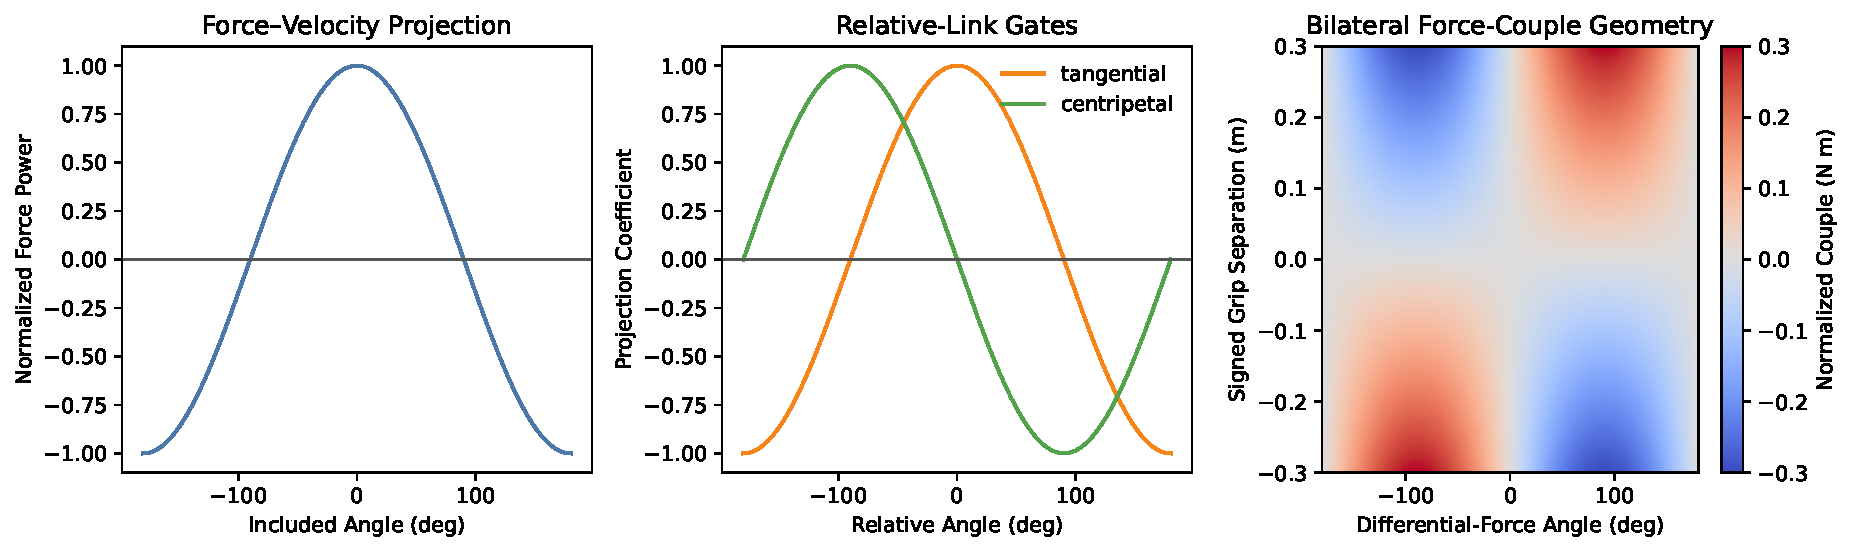
\includegraphics[width=1\linewidth,height=\textheight,keepaspectratio]{figures/fig_momentum_geometry_atlas.pdf}

}

\caption{\label{fig-momentum-geometry-atlas}Geometry Atlas for Force
Power, Relative-Link Projection, and Bilateral Force-Couple Sign.}

\end{figure}%

These are not merely symbolic checks. The existing moving-base planar
control gives exactly zero couple for coincident grips; the
rotating-base tier changes +1.351 to -1.351 N m under signed arm
reversal; and the independently authored MuJoCo and Pinocchio
spatial-contact tier retains a maximum reversal residual below
\(9.2\times10^{-16}\) N m. Proper 3-D rotations preserve total wrench
power to the registered numerical tolerance. The remaining anatomical
question is therefore not whether these geometric identities hold, but
which subject-scaled configurations, forces, velocities, and compliant
contacts are feasible and used by people. The subject-scaled audit in
Section~\ref{sec-subject-scaled-contact-closure} makes that distinction
quantitative: all local constraint Jacobians retain rank six, yet the
prescribed anatomical hand points remain 0.171--0.616 m from the grips.
Full local rank is not contact closure.

The bounded inverse-kinematics follow-up separates unclosed prescription
from reduced-tree reachability. All 234 profile/span/phase
configurations close both point contacts with fixed club coordinates,
rank-six achieved constraint Jacobians, positive engineering-limit
margins, and positive coarse bounding-sphere clearances. That result
clears only the next geometric gate: the bounds are not clinical ranges,
the collision screen is not anatomy, and no contact forces or delivery
outcomes are solved.

\section{Timing and Common Failure
Descriptions}\label{timing-and-common-failure-descriptions}

The terms \emph{casting}, \emph{weak early body acceleration}, and
\emph{late release} are useful only after translation into observables.
The registered timing study therefore treats at least four quantities
independently: proximal-acceleration onset, distal-angle or distal-rate
threshold crossing, proximal-braking onset, and the impact or delivery
event. A result is not robust if it depends on one arbitrary casting
threshold. Work-matched and delivery-state-matched controls are both
required because either matching rule can alter the apparent benefit.

\section{Timing Demand and
Self-Correction}\label{timing-demand-and-self-correction}

A mechanism can be mechanically passive at an instant while its
preparation or regulation remains demanding. Timing demand is therefore
reported as the width or volume of a viable event-time region, outcome
sensitivity to phase error, lower-tail performance, and degradation
under observer delay and noise. Self-correction has the stronger
requirement that a declared physical or feedback mechanism return a
perturbed state toward a viable set. Repeatable open-loop behavior does
not meet that definition.

The delayed-observer experiment makes that distinction executable. Each
policy received the same nuisance parameters and deterministic
sensor-noise realization in an unperturbed reference and a matched
initial-state perturbation. All policies briefly crossed the half-error
threshold in most cases, but most later left it. Requiring sustained
recovery through delivery reduced return fractions to 0.20 for the clock
and delayed/noisy policies and 0.13 for perfect-state and
higher-impedance policies. Median terminal error remained 0.79--0.84 of
the initial perturbation. Figure~\ref{fig-observer-recovery} thus
rejects the shortcut from transient error reduction or low outcome
variance to self-correction; it does not rank human strategies.

\begin{figure}

\centering{

\includegraphics[width=1\linewidth,height=\textheight,keepaspectratio]{figures/fig_observer_recovery.pdf}

}

\caption{\label{fig-observer-recovery}Trajectory-Level Recovery Under
Matched Initial-State Perturbations. Bands show the held-out engineering
envelope; labels above the recovery bars give 90th-percentile
individual-hand force.}

\end{figure}%

The common-phase extension maps both policies onto the same nominal
release coordinate. Clock commands use offsets from 0.140 s; state
thresholds are the right-shoulder angles reached at those same target
times on one common nominal trajectory. The comparison therefore does
not confuse seconds with arbitrary angle thresholds. Six named cohorts
preserve nominal dynamics, a 15\% heavier distal club, 20\% lower shaft
stiffness, 12 ms additional actuator delay, a 50\% larger initial
perturbation, and a combined adverse case. Every policy, load, and phase
has paired reference and perturbed trajectories.

Under the primary task guards---at least 95\% of the load-matched clock
baseline speed, no more than 2 degrees additional face/path error, no
more than 10\% additional peak individual-hand force or squared-torque
effort, and a 5\% normalized numerical-residual ceiling---the clock
policy is viable at four of five phase points across the intersection of
all loads. Its largest contiguous sampled span is 45 ms. The
delayed/noisy state trigger is robustly viable only at the latest point
and therefore has no multi-point span. Strict, primary, and lenient
guards retain the same ordering. Requiring sustained half-error recovery
makes both regions empty: none of the 60 perturbed cases recovers
through delivery. This is evidence against a state-trigger timing or
self-correction advantage in this declared model, not evidence that
people should use clock timing. Half-step checks change delivery speed
by 0.029--0.034 m/s and reduce the normalized residual from 0.014--0.022
to 0.008--0.012.

\begin{figure}

\centering{

\includegraphics[width=1\linewidth,height=\textheight,keepaspectratio]{figures/fig_timing_viability_adverse_load.pdf}

}

\caption{\label{fig-timing-viability-adverse-load}Task Viability and
Realized Trigger Timing Across the Common Phase Grid and Declared
Adverse Loads. Green cells satisfy common speed, face/path, force,
effort, and numerical guards; recovery is reported separately and is
absent in all registered cases.}

\end{figure}%

\section{Proximal Velocity as a Dose, Not a
Maxim}\label{proximal-velocity-as-a-dose-not-a-maxim}

The existing planar evidence is sufficient to reject the rule ``maximize
proximal velocity'' at those declared tiers, but not to specify a human
optimum. An apparent speed benefit must be considered together with
relative motion, control work, interface power, braking work, bilateral
load, club orientation, and the matching rule. The registered analysis
searches explicitly for plateaus, interior optima, and reversals rather
than forcing a monotonic fit. The exact energy-matched state sweep
retains 36 later-phase cases with maximum energy residual
\(5.7\times10^{-14}\) J; no phase is monotonic, and the pre-impact
fitted slope falls from 283.74 to 5.70 W/(rad/s) relative to the
co-varying-energy rule. The initial eight reused work-only pairs favor
the lower-rate member by 4.31--9.28 m/s. The follow-on 216-program
common-time factorial resolves that load confound: its primary
thresholds produce 109 candidate and 46 disjoint work/load-matched
pairs, of which 20 higher-rate members are faster and 26 are slower. All
nine tolerance cells retain both signs. This mixed result rejects a
monotonic rate rule but does not isolate a causal rate effect because
actuator commands and full delivery state differ. The separate 45-case
acceleration intervention holds the entire state and distal torque
fixed. Before impact, increasing proximal acceleration raises interface
power yet reduces club angular acceleration; the required proximal
torque spans -69 to +189 N m. Acceleration is therefore neither a free
input nor a monotonic substitute for proximal rate.

\section{Five Distinct Slack
Hypotheses}\label{five-distinct-slack-hypotheses}

\begin{enumerate}
\def\labelenumi{\arabic{enumi}.}
\tightlist
\item
  \textbf{Contact slack} is temporary loss or weakening of a hand-grip
  constraint.
\item
  \textbf{Transmission slack} is backlash or a dead zone before torque
  transmission.
\item
  \textbf{Structural slack} is compliant preload and elastic
  deformation.
\item
  \textbf{Biological series compliance} is a muscle-tendon state with
  stored and released energy.
\item
  \textbf{Control slack} is an activation deadband, delay, or
  co-contraction reserve.
\end{enumerate}

The dynamic constitutive audit now exercises all five classes separately
under a slow closed-cycle sine and a richer multisine with repeated
reversals. The four mechanical surrogates satisfy the registered
passivity and work-energy closure checks; the largest absolute closure
residual is \(5.13\times10^{-10}\) J. The control deadband is
deliberately treated as a delayed command-transmission map, so
mechanical passivity and stored energy are not assigned to it.

The richer excitation improves the local scaled-sensitivity conditioning
of every mechanical surrogate. Each three-parameter local Jacobian is
full rank, but that result does not identify the generating class. Under
the registered multisine, contact disengagement and the
biological-compliance surrogate differ by only 1.96\% normalized
transmitted-output RMSE. Independent contact, tissue, shaft, activation,
and bilateral-wrench measurements are therefore necessary to distinguish
mechanisms rather than fitting one output channel. The transmission
element remains a memoryless dead-zone-plus-damping surrogate, not a
stateful rate-independent play operator, and the biological element is a
unilateral Kelvin-Voigt surrogate rather than a subject-specific tendon
model.

\begin{figure}

\centering{

\includegraphics[width=1\linewidth,height=\textheight,keepaspectratio]{figures/fig_typed_slack_dynamic_audit.pdf}

}

\caption{\label{fig-typed-slack-dynamic-audit}Typed Slack Dynamic Audit.
Mechanical force-displacement loops, the delayed control boundary, local
scaled-sensitivity ranks, and normalized outputs are shown for the
registered synthetic excitations.}

\end{figure}%

This evidence supports only a typed experimental program. It does not
show that slack is good, bad, intentional, required, or beneficial for
delivery. The articulated forward atlas now performs the first of those
transport tests: bilateral, tension-only, and two dead-zone laws are
compared under common displacement and approximately matched radial
extension across 1,944 bounded trajectories. The 1.5 mm law remains open
under the common 1 mm displacement but taut under matched extension;
natural branches show no transition before 5 ms, while isolated boundary
probes qualify opening and reattachment. This shows why preload matching
changes the answer, not that either condition is beneficial. Any benefit
proposal must still survive longer matched-work/load delivery, stateful
hysteresis, calibrated distributed contact, and independent human
measurement.

The next articulated atlas crosses frictionless and
equipment-provisional \(\mu=0.35\) tension-fiber comparators with one,
three, and five stations per hand while holding total stiffness and
damping fixed. Its 576 trajectories pass nested 4, 10, 25, and 50 ms
power, energy, refinement, geometry-null, and MuJoCo--Pinocchio gates.
Separate probes record opening and reattachment with exact engine
agreement, but begin disengaged and do not qualify an attached-to-open
first failure. Finite-friction minus frictionless 50 ms speed
differences have mixed signs. The result therefore demonstrates
sensitivity, not a physical benefit of friction, slack, or distributed
pressure. A mass-metric impulsive perfect-stick control bounds
instantaneous kinetic-energy capture at
\(9.84\times10^{-9}\)--\(0.37665\) J while enforcing tangential velocity
below \(9.65\times10^{-11}\) m/s with exact stored-precision engine
parity. It does not test static-friction feasibility or subsequent
stick--slip evolution. Attached-to-open first failure, measured contact,
coupled shaft/ground work, matched tasks, and governed human outcomes
remain necessary.

The following articulated shaft atlas then retains the five-fiber grip
and adds rigid, bending-only, torsion-only, and coupled passive-club
branches. Its 384 trajectories pass the registered 0.25/0.125 ms
work--energy, small-deformation, killswitch, and native-engine gates
through 50 ms; 1.0 and 0.50 ms torsion probes fail closed outside the
declared linear domain. Of 384 coupled--rigid cells, 126 meet the
predeclared 5\% peak-load and dissipated-work match. Their final-speed
differences include 82 negative and 44 positive values. Passive shaft
response is therefore a state-dependent pathway in this synthetic model,
not a general speed advantage. Equipment calibration, higher mode
adequacy under fast loading, ground work, impact, and human outcomes
remain open.

\section{Evidential Boundary}\label{evidential-boundary}

These experiments are designed to make the framework easier to disprove.
Synthetic studies can reject a mechanism within a declared model and can
qualify software, but they cannot establish a coaching instruction or
human control strategy. The participant-held-out stage remains blocked
until a governed dataset contains synchronized full-body and club
kinematics, force plates, bilateral six-axis grip wrenches, grip/contact
state, and impact outcomes. Substituting synthetic traces would erase
the question the human stage is intended to answer.

\section{Point-by-Point Readiness
Audit}\label{point-by-point-readiness-audit}

The handwritten agenda contains nine testable points after its nested
timing examples are separated: drift contribution; geometry; casting;
early-downswing proximal acceleration; segment release; timing
precision; self-correction and noise robustness; proximal-velocity
maximization; and slack. The executable readiness audit preserves all
nine rather than allowing a broad question to hide an unplanned
subquestion. Eight presently have a model-bounded answer or a negative
general-rule result. The unresolved point is the broader
timing-precision claim: the registered planar comparison is adverse to a
state-trigger advantage, but spatial and human timing demand remain
untested. All nine have a registered model experiment and a
participant-held-out human stage, but the latter remains blocked by the
bilateral-wrench data boundary.

The machine-readable authority is
\href{../data/momentum_transfer_readiness_audit.json}{\texttt{momentum\_transfer\_readiness\_audit.json}}.
It is regenerated from the question and experiment registries and
validated in CI. A missing source point, missing falsifier, invalid
evidence status, absent human stage, or experiment linked to the wrong
question is a hard failure.

\begingroup
\small

\begin{longtable}[]{@{}
  >{\raggedright\arraybackslash}p{(\linewidth - 4\tabcolsep) * \real{0.2400}}
  >{\raggedright\arraybackslash}p{(\linewidth - 4\tabcolsep) * \real{0.3600}}
  >{\raggedright\arraybackslash}p{(\linewidth - 4\tabcolsep) * \real{0.4000}}@{}}
\caption{Readiness assessment for every point transcribed from the
source agenda. ``Partly answered'' never denotes a human or coaching
conclusion. }\label{tbl-momentum-source-readiness}\tabularnewline
\toprule\noalign{}
\begin{minipage}[b]{\linewidth}\raggedright
Source Point
\end{minipage} & \begin{minipage}[b]{\linewidth}\raggedright
Present Scientific State
\end{minipage} & \begin{minipage}[b]{\linewidth}\raggedright
Next Decisive Model Test
\end{minipage} \\
\midrule\noalign{}
\endfirsthead
\toprule\noalign{}
\begin{minipage}[b]{\linewidth}\raggedright
Source Point
\end{minipage} & \begin{minipage}[b]{\linewidth}\raggedright
Present Scientific State
\end{minipage} & \begin{minipage}[b]{\linewidth}\raggedright
Next Decisive Model Test
\end{minipage} \\
\midrule\noalign{}
\endhead
\bottomrule\noalign{}
\endlastfoot
Drift contribution & Partly answered; observable- and window-specific
only & Common cross-tier estimand table with uncertainty \\
Geometry dependencies & Partly answered through reduced spatial
controls; the first subject-scaled audit rejects contact feasibility of
the prescribed common states & Closed-contact inverse kinematics,
calibrated contact, and independent forward integration \\
Casting & Partly answered: no single event definition is defensible;
human causal interpretation remains open & Multiple preregistered event
definitions under matched controls \\
Early proximal acceleration & Partly answered pointwise; nonmonotonic &
Forward factorial intervention with full-state/work/load matching \\
Segment release & Partly answered; objective- and constraint-dependent &
Viable-region mapping across proximal and distal control families \\
Timing precision & Unresolved beyond an adverse planar result; a
state-trigger volume advantage is not supported in the registered planar
tier & Continuous common-phase spatial and subject-scaled comparison \\
Self-correction and noise robustness & Partly answered negatively at the
registered planar tier; no sustained recovery in 60 cases & Continuous
attraction regions with identified observers and external-contact
loads \\
Proximal-velocity maximization & Not supported as a general planar rule
& Causal full-delivery-state-matched spatial dose response \\
Slack & Partly answered at a synthetic constitutive tier; no global
benefit and one-channel class identification is not established &
One-class-at-a-time moving-base and spatial delivery tests with stateful
backlash, subject-specific tissue, and independent measurements \\
\end{longtable}

\endgroup

\chapter{Conclusions and Research Priorities}\label{sec-conclusions}

\section{Conclusions}\label{conclusions}

The literature does not support equating proximal-to-distal peak order
with a requirement to transfer mechanical energy outward as early as
possible. Interaction dynamics, optimal-control studies, and segmental
energy measurements instead motivate a timing hypothesis: retain a
compact proximal configuration while proximal speed develops, then
accelerate the distal handoff later in the downswing.

The present simulations provide model-derived support for that
mechanism. Under matched shoulder torque in a planar two-link model,
early wrist drive reduced clubhead speed relative to a passive wrist,
whereas grid-selected late drive increased it. A small early restraining
torque followed by late drive was best among the tested programs. Energy
and counterfactual accounting located the modeled mechanism in early
arm-energy retention and late joint-force transfer rather than in early
active wrist work.

This conclusion is conditional. The result survived torque-velocity
bounds, alternative scoring rules, 13 one-at-a-time parameter cases, and
declared 20--50 ms command transitions, but the selected onset shifted
across cases. The study therefore supports a robust ordering within a
local model neighborhood, not a universal timing value or an individual
coaching prescription. Planar motion, simplified actuators, and absence
of human data remain material limitations. The finite sweep is not a
continuous optimal-control solution, and the command filters are not
muscle activation models.

The forward constrained two-hand extension resolves one previously open
mechanistic question. Starting from the exact same 0.200 s state, the
force-generated club couple remains negative for 50 ms after all applied
joint torques are removed. The effect disappears exactly when both grip
moment arms are removed and remains stable under timestep and projection
refinement. This supports finite passive-couple persistence in the
declared planar model, not a claim about muscle inactivity or human
technique.

The coupled moving-base/flexible-club extension resolves the next
structural question at the planar tier. Base translation, shaft flex,
and both grip forces evolve in one forward constrained solve. The
negative force-generated couple survives the same-state zero-command
intervention, while coincident grip points remove it exactly;
constraint, contact-power, and work--energy residuals close under
timestep refinement. This transports the mechanism beyond a fixed base
and rigid club without promoting it to a spatial or physiological
result.

The distributed-shaft comparison closes a narrower structural gate. A
one-mode reduction and six-mode Euler--Bernoulli reference share the
same assembled mass, stiffness, damping, tip inertia, and loads. The
reduced model closely follows slow loading but misses higher-mode
history under a short force-and-moment pulse, even when their peak
deflections are similar. Synthetic modal identification, mesh
convergence, and work--energy closure pass. This does not calibrate
equipment or show that the result survives coupling the beam into the
two-hand constrained solve.

The articulated finite-base extension closes the next numerical
mechanism gate while producing an adverse primary inference result.
Across 384 pathway and 192 independent-control trajectories, the native
inertia-and-bias operators remain within the registered transport
bounds, energy residuals decrease with step refinement, and all declared
shaft/base domains hold through 50 ms. Ground force and intrinsic free
moment are mechanically active, but none of 384 coupled--fixed
comparisons meets the preregistered 5\% peak-load and
total-dissipated-work match. A post-hoc non-ground-dissipation
sensitivity admits 60 cells with both speed-difference signs. The
experiment therefore qualifies finite-base coupling and rejects a
universal delivery interpretation; it does not identify a ground-use
strategy or human benefit.

The reduced full-body common-state extension resolves implementation
transport for a narrower spatial estimand. MuJoCo and an independent
Lagrange--Christoffel formulation agree across 20 coordinates and 61
nonplanar states to \(2.14\times10^{-11}\) relative error. Reversing the
hand moment arm reverses the force-generated couple and coincident
points remove it exactly. Because the forces are prescribed and the
state is shared, this supports spatial inverse-dynamics and geometry
transport but leaves passive forward contact inconclusive at that tier.

The subject-scaled contact-closure audit rejects a tempting shortcut at
that same tier. Six deterministic de Leva profiles retain a
full-row-rank local contact Jacobian, yet the prescribed anatomical hand
points remain 0.171--0.616 m from the declared grips. Rank and
conditioning therefore cannot substitute for closed feasible anatomy.
The next articulated spatial tier must solve bilateral closed-contact
inverse kinematics with joint-limit and collision checks before its
forward contact, timing, recovery, or slack results can be interpreted.
The registered inverse-kinematics follow-up now clears that reduced-tree
gate in all 234 profile/span/phase samples while holding the club pose
fixed. Its minimum engineering-limit margin is 0.103 rad and its minimum
coarse bounding-sphere clearance is 30.9 mm. These are screening
results, not measured anatomical ranges or mesh-level clearance; they
advance the next test to calibrated compliant forward contact from the
closed states.

A paired arm-only intervention now isolates one omitted structure. With
trunk and club pose fixed, the fixed-shoulder branch closes none of 54
registered states, whereas a bounded scapula-on-ellipsoid surrogate
reaches the contact residual in 31 states and satisfies both residual
and solver-termination gates in 16. Full rank persists while coordinate
nullity rises from two to ten, so the result supports the importance of
scapular geometry but also strengthens the non-identifiability boundary.
It is not an anatomical, muscular, or human strategy result.

The reduced spatial forward-contact extension resolves that narrower
mechanism gate. Native MuJoCo and Pinocchio independently supply
rigid-body kinematics, mass, bias, gravity, and continuous-time
acceleration for two finite-mass hand carriages and a free rigid club
without direct club actuation. Both branches share the projected
compliant interfaces and project-authored state update. Their baseline
and same-state killswitch trajectories satisfy the declared position,
orientation, wrench, and energy regions. Removing the complete grounded
driver leaves a negative force-generated swing-normal couple for 37.5 ms
in both engines; coincident and reversed-moment-arm controls close
exactly, and the work--energy residual decreases under timestep
refinement. This supports reduced spatial contact persistence and
inertia-and-bias transport, not independent contact-solver equivalence,
anatomical arms, muscles, calibrated grip tissue, equipment, or human
strategy. A separate MuJoCo-native equality and \texttt{mj\_step}
control produces a nonzero discrepancy from the projected formulation
and is reported as a formulation difference, not a parity success.

The closed-state validity-horizon extension further shows that the same
two engines remain inside the declared trajectory, wrench,
energy-discrepancy, and work--energy closure gates for all 2,160
registered cases through 50 ms. The matrix spans all
profile--span--phase states plus one-factor stiffness, damping,
hand-mass, timestep, and immediate-driver-off branches. No failure is
observed inside the registered interval, so the result is right-censored
at 50 ms. It strengthens the reduced numerical reference but does not
turn the hand-carriage model into articulated anatomy or a full delivery
simulation.

The coupled uncertainty/control phase rejects two additional shortcuts.
A net planar wrench cannot uniquely identify both hand forces, and six
summary observables cannot identify the complete 12-parameter vector.
Separate training and held-out ensembles leave objective-dependent
tradeoffs among all eight command programs. Early restraint improves
held-out lower-tail speed relative to late drive but increases the
planar face/path error, so the result supports a conditional model
mechanism rather than a universal or physiological strategy.

The experimental phase is preregistered but not empirically executed.
Its machine-readable protocol fixes six synchronized modalities,
participant-level holdout, identity-safe provenance, filtering and
residual sensitivities, and four prediction-specific falsifiers. The
synthetic dry run passes all intake and fail-closed controls, but it
cannot advance H1--H4. Governed human data are still required.

The open-resource layer now supplies model-tier presets, a hash-pinned
release manifest, standard checksums, a data dictionary, citation
metadata, and a claim-first reviewer workbench. Validation fails closed
on artifact drift. The bundle remains a qualified local release
candidate rather than a persistent archive: articulated subject-scaled
contact, equipment-calibrated beam coupling, governed human evaluation,
and external identifier deposit remain open.

\section{Research Priorities}\label{sec-future}

The next work should reduce the largest inferential risks in dependency
order:

\begin{enumerate}
\def\labelenumi{\arabic{enumi}.}
\tightlist
\item
  \textbf{Articulated Spatial Forward-Contact Counterfactual.} Replace
  the executed hand-carriage reference with subject-scaled articulated
  arms and calibrated grip interfaces. Start from the executed bilateral
  closed-contact, engineering-limit, and coarse collision-qualified
  configurations, replace those screens with subject-specific anatomy
  where available, then preserve the two-engine same-state killswitch,
  force, couple, power, work, pathway, and closure observables.
\item
  \textbf{Calibrated Uncertainty and Constrained Control.} Extend the
  executed multivariable screen with population-informed distributions,
  measurement error, profile-likelihood or Bayesian calibration, larger
  held-out ensembles, and a constrained optimal-control comparator.
\item
  \textbf{Spatial Model-Fidelity Ladder.} Extend the executed planar
  base rotation, intrinsic free moment, distributed grip, and passive
  shaft into a three- dimensional club/body solve with calibrated
  unilateral foot contact and force-plate comparison without changing
  the registered interface observables. Each rung should carry
  conservation checks and cross-engine tolerance gates.
\item
  \textbf{Execute the Frozen Human-Data Protocol.} Acquire governed
  synchronized measurements that pass the fixed inclusion, residual,
  missingness, participant-holdout, and provenance gates. Sequence order
  alone must not be treated as evidence of energy transfer.
\item
  \textbf{Arm--Wrist Allocation and Preload Falsification.} Execute the
  bilateral grip-wrench, pressure, activation, stiffness, and
  participant-holdout tests registered in
  Section~\ref{sec-torque-allocation-preload}. Treat the dead-zone
  mechanism as rejected if its predicted gap is absent under documented
  low tangent stiffness or if any performance difference disappears on
  holdout.
\item
  \textbf{Open-Resource Release.} Maintain deterministic commands,
  machine-readable results, data dictionaries, checksums, citation
  metadata, and explicit license boundaries. Archive validated releases
  with a persistent identifier.
\end{enumerate}

The implementation roadmap and acceptance criteria are tracked in
\href{https://github.com/D-sorganization/UpstreamDrift/issues/8426}{the
open research epic}. The matched-task allocation and transmission
program is tracked separately in
\href{https://github.com/D-sorganization/UpstreamDrift/issues/8497}{its
falsification epic}.

\chapter*{Code and Data Availability}\label{code-and-data-availability}
\addcontentsline{toc}{chapter}{Code and Data Availability}

Analysis code, tests, figures, machine-readable outputs, and parameter
records are available in the
\href{https://github.com/D-sorganization/UpstreamDrift/tree/main/docs/research/proximal_distal_energy_transfer}{open-source
repository}. The repository name identifies provenance only; none of the
scientific claims depend on adoption of the broader software project.
The principal summary is recorded in
\href{https://github.com/D-sorganization/UpstreamDrift/blob/main/docs/research/proximal_distal_energy_transfer/data/results_summary.json}{\texttt{data/results\_summary.json}},
and the parameter-sensitivity results are recorded in
\href{https://github.com/D-sorganization/UpstreamDrift/blob/main/docs/research/proximal_distal_energy_transfer/data/e1d_parameter_sensitivity.json}{\texttt{data/e1d\_parameter\_sensitivity.json}}.
The spatial common-state evidence is recorded in
\href{https://github.com/D-sorganization/UpstreamDrift/blob/main/docs/research/proximal_distal_energy_transfer/data/spatial_full_body_study.json}{\texttt{data/spatial\_full\_body\_study.json}}.
The two-engine spatial forward-contact evidence is recorded in
\href{https://github.com/D-sorganization/UpstreamDrift/blob/main/docs/research/proximal_distal_energy_transfer/data/spatial_forward_contact_study.json}{\texttt{data/spatial\_forward\_contact\_study.json}}.
The uncertainty, identifiability, and control evidence is recorded in
\href{https://github.com/D-sorganization/UpstreamDrift/blob/main/docs/research/proximal_distal_energy_transfer/data/uncertainty_control_study.json}{\texttt{data/uncertainty\_control\_study.json}}.
The distributed-shaft structural evidence is recorded in
\href{https://github.com/D-sorganization/UpstreamDrift/blob/main/docs/research/proximal_distal_energy_transfer/data/shaft_beam_reference.json}{\texttt{data/shaft\_beam\_reference.json}}.
The forward distributed-modal shaft and arm--wrist allocation evidence
are recorded in
\href{https://github.com/D-sorganization/UpstreamDrift/blob/main/docs/research/proximal_distal_energy_transfer/data/moving_base_modal_shaft_study.json}{\texttt{data/moving\_base\_modal\_shaft\_study.json}}
and
\href{https://github.com/D-sorganization/UpstreamDrift/blob/main/docs/research/proximal_distal_energy_transfer/data/torque_allocation_preload_study.json}{\texttt{data/torque\_allocation\_preload\_study.json}}.
The frozen experimental protocol and synthetic readiness classification
are recorded in
\href{https://github.com/D-sorganization/UpstreamDrift/blob/main/docs/research/proximal_distal_energy_transfer/data/experimental_protocol_v1.json}{\texttt{data/experimental\_protocol\_v1.json}}
and
\href{https://github.com/D-sorganization/UpstreamDrift/blob/main/docs/research/proximal_distal_energy_transfer/data/experimental_protocol_readiness.json}{\texttt{data/experimental\_protocol\_readiness.json}}.
The finite-ground initialization, preregistered atlas, and labeled
post-hoc matching sensitivity are recorded in
\href{https://github.com/D-sorganization/UpstreamDrift/blob/main/docs/research/proximal_distal_energy_transfer/data/articulated_ground_diagnostic.json}{\texttt{data/articulated\_ground\_diagnostic.json}},
\href{https://github.com/D-sorganization/UpstreamDrift/blob/main/docs/research/proximal_distal_energy_transfer/data/articulated_ground_atlas.json}{\texttt{data/articulated\_ground\_atlas.json}},
and
\href{https://github.com/D-sorganization/UpstreamDrift/blob/main/docs/research/proximal_distal_energy_transfer/data/articulated_ground_posthoc_sensitivity.json}{\texttt{data/articulated\_ground\_posthoc\_sensitivity.json}}.

\section{Normalized Claim
Adjudication}\label{normalized-claim-adjudication}

The current census contains 328 material claims. The normalized outcome
applies only to each claim's declared estimand, model domain, and
uncertainty boundary. A \texttt{supported} model-conditional claim is
not thereby independently replicated, empirically validated, or
converted into a human strategy recommendation.

The absence of a \texttt{contradicted} row does not mean that every
mechanism survived every adverse test. Claims that accurately report
null, mixed, or adverse model results can themselves be supported. The
complete finding-level reasons, falsifiers, locators, and boundaries are
available in the
\href{https://github.com/D-sorganization/UpstreamDrift/blob/main/docs/research/proximal_distal_energy_transfer/data/claim_adjudication_summary.json}{reviewer
JSON} and
\href{https://github.com/D-sorganization/UpstreamDrift/blob/main/docs/research/proximal_distal_energy_transfer/data/claim_adjudication_summary.csv}{reviewer
CSV}.

\subsection{Outcome Counts}\label{outcome-counts}

\begin{longtable}[]{@{}lr@{}}
\caption{Outcome Counts for the Current Claim
Census.}\label{tbl-claim-outcomes}\tabularnewline
\toprule\noalign{}
Normalized Outcome & Claim Count \\
\midrule\noalign{}
\endfirsthead
\toprule\noalign{}
Normalized Outcome & Claim Count \\
\midrule\noalign{}
\endhead
\bottomrule\noalign{}
\endlastfoot
\texttt{inconclusive} & 5 \\
\texttt{supported} & 308 \\
\texttt{untested} & 15 \\
\end{longtable}

\newpage

\subsection{Evidence Tier Counts}\label{evidence-tier-counts}

\begin{longtable}[]{@{}lr@{}}
\caption{Evidence Tier Counts for the Current Claim
Census.}\label{tbl-claim-evidence-tiers}\tabularnewline
\toprule\noalign{}
Evidence Tier & Claim Count \\
\midrule\noalign{}
\endfirsthead
\toprule\noalign{}
Evidence Tier & Claim Count \\
\midrule\noalign{}
\endhead
\bottomrule\noalign{}
\endlastfoot
\texttt{bibliographic\_record} & 3 \\
\texttt{external\_empirical\_human} & 34 \\
\texttt{external\_methods\_or\_measurement} & 10 \\
\texttt{external\_modeling\_or\_simulation} & 15 \\
\texttt{external\_review\_or\_synthesis} & 10 \\
\texttt{project\_derivation\_or\_document} & 113 \\
\texttt{project\_executable\_or\_generated} & 299 \\
\texttt{prospective\_or\_unexecuted} & 15 \\
\end{longtable}

\subsection{Source Independence
Counts}\label{source-independence-counts}

\begin{longtable}[]{@{}lr@{}}
\caption{Source Independence Counts for the Current Claim
Census.}\label{tbl-claim-source-independence}\tabularnewline
\toprule\noalign{}
Source Independence & Claim Count \\
\midrule\noalign{}
\endfirsthead
\toprule\noalign{}
Source Independence & Claim Count \\
\midrule\noalign{}
\endhead
\bottomrule\noalign{}
\endlastfoot
\texttt{multiple\_independent\_external\_support} & 20 \\
\texttt{project\_only} & 274 \\
\texttt{single\_independent\_external\_support} & 34 \\
\end{longtable}

\subsection{Model Tier Counts}\label{model-tier-counts}

\begin{longtable}[]{@{}lr@{}}
\caption{Model Tier Counts for the Current Claim
Census.}\label{tbl-claim-model-tiers}\tabularnewline
\toprule\noalign{}
Model Tier & Claim Count \\
\midrule\noalign{}
\endfirsthead
\toprule\noalign{}
Model Tier & Claim Count \\
\midrule\noalign{}
\endhead
\bottomrule\noalign{}
\endlastfoot
\texttt{articulated\_spatial} & 35 \\
\texttt{compliant\_shaft} & 66 \\
\texttt{cross\_tier\_synthesis} & 77 \\
\texttt{declared\_model\_tier\_unclassified} & 12 \\
\texttt{finite\_ground\_or\_base} & 16 \\
\texttt{human\_or\_external\_evidence} & 46 \\
\texttt{planar\_reduced} & 150 \\
\texttt{spatial\_reduced} & 76 \\
\texttt{two\_hand\_or\_bilateral} & 94 \\
\texttt{uncertainty\_or\_control} & 10 \\
\end{longtable}

\subsection{Unresolved Replication
Counts}\label{unresolved-replication-counts}

\begin{longtable}[]{@{}lr@{}}
\caption{Unresolved Replication Counts for the Current Claim
Census.}\label{tbl-claim-replication}\tabularnewline
\toprule\noalign{}
Replication Class & Claim Count \\
\midrule\noalign{}
\endfirsthead
\toprule\noalign{}
Replication Class & Claim Count \\
\midrule\noalign{}
\endhead
\bottomrule\noalign{}
\endlastfoot
\texttt{external\_validation\_open} & 1 \\
\texttt{full\_text\_or\_original\_source\_open} & 5 \\
\texttt{governed\_human\_data\_unavailable} & 11 \\
\texttt{independent\_reimplementation\_open} & 12 \\
\texttt{mixed\_or\_insufficient\_evidence} & 5 \\
\texttt{none\_declared} & 284 \\
\texttt{prospective\_experiment\_open} & 15 \\
\texttt{statistical\_reanalysis\_or\_replication\_open} & 9 \\
\texttt{systematic\_review\_open} & 2 \\
\end{longtable}

\newpage

\subsection{Claim-Family Source
Concentration}\label{claim-family-source-concentration}

\begin{longtable}[]{@{}
  >{\raggedright\arraybackslash}p{(\linewidth - 6\tabcolsep) * \real{0.2143}}
  >{\raggedleft\arraybackslash}p{(\linewidth - 6\tabcolsep) * \real{0.2857}}
  >{\raggedleft\arraybackslash}p{(\linewidth - 6\tabcolsep) * \real{0.2857}}
  >{\raggedright\arraybackslash}p{(\linewidth - 6\tabcolsep) * \real{0.2143}}@{}}
\caption{Claim-Family Source Concentration Flags; the tuple is project
only / one independent work / two or more independent
works.}\label{tbl-claim-family-concentration}\tabularnewline
\toprule\noalign{}
\begin{minipage}[b]{\linewidth}\raggedright
Claim Family
\end{minipage} & \begin{minipage}[b]{\linewidth}\raggedleft
Claims
\end{minipage} & \begin{minipage}[b]{\linewidth}\raggedleft
Source-Category Tuple
\end{minipage} & \begin{minipage}[b]{\linewidth}\raggedright
Flag
\end{minipage} \\
\midrule\noalign{}
\endfirsthead
\toprule\noalign{}
\begin{minipage}[b]{\linewidth}\raggedright
Claim Family
\end{minipage} & \begin{minipage}[b]{\linewidth}\raggedleft
Claims
\end{minipage} & \begin{minipage}[b]{\linewidth}\raggedleft
Source-Category Tuple
\end{minipage} & \begin{minipage}[b]{\linewidth}\raggedright
Flag
\end{minipage} \\
\midrule\noalign{}
\endhead
\bottomrule\noalign{}
\endlastfoot
ch01 introduction & 2 & 0 / 2 / 0 & external support concentrated \\
ch02 mechanics & 33 & 5 / 17 / 11 & mixed independence \\
ch03 evidence & 14 & 1 / 10 / 3 & mixed independence \\
ch03 interaction forces & 10 & 8 / 1 / 1 & mixed independence \\
ch03b hand path attribution & 11 & 7 / 2 / 2 & mixed independence \\
ch03ba coordinate force sources & 3 & 3 / 0 / 0 & project authored
only \\
ch03c ground reaction drift & 8 & 4 / 2 / 2 & mixed independence \\
ch03d shoulder velocity transfer & 18 & 18 / 0 / 0 & project authored
only \\
ch04 counterfactual ensemble & 6 & 6 / 0 / 0 & project authored only \\
ch04 counterfactuals & 5 & 4 / 0 / 1 & mixed independence \\
ch05 two hand wrench & 21 & 21 / 0 / 0 & project authored only \\
ch05a interactive workbench & 1 & 1 / 0 / 0 & project authored only \\
ch05b forward two hand & 15 & 15 / 0 / 0 & project authored only \\
ch06 shaft contributions & 15 & 15 / 0 / 0 & project authored only \\
ch06b coupled base flex & 14 & 14 / 0 / 0 & project authored only \\
ch06bb shaft beam reference & 2 & 2 / 0 / 0 & project authored only \\
ch06bbb forward modal shaft & 7 & 7 / 0 / 0 & project authored only \\
ch06bc torque allocation preload & 7 & 7 / 0 / 0 & project authored
only \\
ch06c spatial cross formulation & 44 & 44 / 0 / 0 & project authored
only \\
ch06ca articulated ground & 1 & 1 / 0 / 0 & project authored only \\
ch06cb spatial cross tail & 6 & 6 / 0 / 0 & project authored only \\
ch06cc spatial forward contact & 8 & 8 / 0 / 0 & project authored
only \\
ch06cd articulated attribution & 3 & 3 / 0 / 0 & project authored
only \\
ch06d uncertainty control & 10 & 10 / 0 / 0 & project authored only \\
ch06e experimental protocol & 1 & 1 / 0 / 0 & project authored only \\
ch06f open release & 2 & 2 / 0 / 0 & project authored only \\
ch07 model ladder & 32 & 32 / 0 / 0 & project authored only \\
ch07 results & 7 & 7 / 0 / 0 & project authored only \\
ch07b frames biology engines & 5 & 5 / 0 / 0 & project authored only \\
ch07c transmission robustness & 5 & 5 / 0 / 0 & project authored only \\
ch08b momentum transfer questions & 10 & 10 / 0 / 0 & project authored
only \\
ch09 conclusions & 2 & 2 / 0 / 0 & project authored only \\
\end{longtable}

Evidence-tier, model-tier, and unresolved-replication labels are
nonexclusive, so those totals can exceed the claim count. Source
independence is an exact one-category partition derived from the
canonical-work review. No governed participant outcome is present; human
validation remains an external-data boundary.

\chapter{Software and Data Availability}\label{sec-appendix-inventory}

The open-source implementation separates the analytical model, torque
programs, counterfactual evaluation, energy accounting, robustness
analyses, and figure generation. The scientific entry points are
collected under
\href{https://github.com/D-sorganization/UpstreamDrift/tree/main/scripts/research/proximal_distal_energy}{\texttt{scripts/research/proximal\_distal\_energy/}},
with shared model parameters and dynamics under
\href{https://github.com/D-sorganization/UpstreamDrift/tree/main/src/shared/python/simulation_backends}{\texttt{simulation\_backends/}}.
This is a provenance statement, not a capability claim about the
surrounding software.

The current evidence boundary includes these known limitations:

\begin{itemize}
\tightlist
\item
  A multi-phase matched-state torque-killswitch ensemble is complete for
  one declared torque program; other torque programs, model classes, and
  uncertainty distributions remain necessary before making general
  persistence claims.
\item
  The archived two-hand ZTCF remains pointwise along the BASE state
  history. Separate forward rigid-club and coupled
  moving-base/flexible-club models now demonstrate finite zero-command
  persistence. A reduced full-body spatial common-state tier now tests
  nonplanar inverse dynamics, but passive spatial contact and human
  variants remain open validation steps.
\item
  The primary model has two planar links and a fixed hub; torso,
  hub-path, long-axis rotation, and closed-loop arm effects are absent.
\item
  The shaft extension is a three-coordinate point-mass surrogate with
  one linear torsional mode. It is not a calibrated distributed-beam or
  equipment model, and extreme low-stiffness deflections exceed its
  linear premise.
\item
  The coupled actuator adds delay, first-order activation, rate and
  torque--velocity limits, and impedance, but it remains a
  nonphysiological command surrogate.
\item
  Coupled uncertainty is screened over declared engineering envelopes;
  population distributions and measurement uncertainty are not
  estimated.
\item
  No human motion or force data are analyzed; the result is mechanistic
  and model-derived, not a skill-group effect.
\item
  The model ladder now executes reduced and subject-scaled forward
  two-hand contact, distributed grip, passive first-mode shaft, and
  planar finite-base ground/free-moment tiers in MuJoCo and Pinocchio.
  The interfaces and support law remain synthetic, bilateral, and
  uncalibrated; three-dimensional unilateral foot contact and governed
  human validation remain unexecuted.
\end{itemize}

\chapter{Reproducibility Guide}\label{sec-appendix-repro}

From the repository root (Python 3.11+ with the project dependencies):

\begin{Shaded}
\begin{Highlighting}[]
\CommentTok{\# Primary sweep, counterfactuals, and interface{-}power analysis}
\ExtensionTok{python3} \AttributeTok{{-}m}\NormalTok{ scripts.research.proximal\_distal\_energy.run\_experiments}

\CommentTok{\# Registered WSCG source extraction and interaction{-}force analysis}
\ExtensionTok{python3} \AttributeTok{{-}m}\NormalTok{ scripts.research.proximal\_distal\_energy.extract\_wscg\_charts}
\ExtensionTok{python3} \AttributeTok{{-}m}\NormalTok{ scripts.research.proximal\_distal\_energy.run\_interaction\_force\_study}
\ExtensionTok{python3} \AttributeTok{{-}m}\NormalTok{ scripts.research.proximal\_distal\_energy.run\_counterfactual\_ensemble}
\ExtensionTok{python3} \AttributeTok{{-}m}\NormalTok{ scripts.research.proximal\_distal\_energy.run\_two\_hand\_wscg\_analysis}
\ExtensionTok{python3} \AttributeTok{{-}m}\NormalTok{ scripts.research.proximal\_distal\_energy.run\_shaft\_contribution\_study}
\ExtensionTok{python3} \AttributeTok{{-}m}\NormalTok{ scripts.research.proximal\_distal\_energy.run\_mechanism\_ladder\_study}
\ExtensionTok{python3} \AttributeTok{{-}m}\NormalTok{ scripts.research.proximal\_distal\_energy.run\_forward\_two\_arm\_study}
\ExtensionTok{python3} \AttributeTok{{-}m}\NormalTok{ scripts.research.proximal\_distal\_energy.run\_moving\_base\_flexible\_study}
\ExtensionTok{python3} \AttributeTok{{-}m}\NormalTok{ scripts.research.proximal\_distal\_energy.run\_shaft\_beam\_reference}
\ExtensionTok{python3} \AttributeTok{{-}m}\NormalTok{ scripts.research.proximal\_distal\_energy.run\_spatial\_full\_body\_study}
\ExtensionTok{python3} \AttributeTok{{-}m}\NormalTok{ scripts.research.proximal\_distal\_energy.run\_articulated\_manufactured\_solution}
\ExtensionTok{python3} \AttributeTok{{-}m}\NormalTok{ scripts.research.proximal\_distal\_energy.run\_articulated\_native\_constraint\_discrepancy}
\ExtensionTok{python3} \AttributeTok{{-}m}\NormalTok{ scripts.research.proximal\_distal\_energy.make\_articulated\_native\_constraint\_discrepancy\_figure}
\ExtensionTok{python3} \AttributeTok{{-}m}\NormalTok{ scripts.research.proximal\_distal\_energy.run\_articulated\_ground\_diagnostic}
\ExtensionTok{python3} \AttributeTok{{-}m}\NormalTok{ scripts.research.proximal\_distal\_energy.run\_articulated\_ground\_atlas}
\ExtensionTok{python3} \AttributeTok{{-}m}\NormalTok{ scripts.research.proximal\_distal\_energy.run\_articulated\_ground\_posthoc\_sensitivity}
\ExtensionTok{python3} \AttributeTok{{-}m}\NormalTok{ scripts.research.proximal\_distal\_energy.run\_uncertainty\_control\_study}
\ExtensionTok{python3} \AttributeTok{{-}m}\NormalTok{ scripts.research.proximal\_distal\_energy.run\_experimental\_protocol\_dry\_run}
\ExtensionTok{python3} \AttributeTok{{-}m}\NormalTok{ scripts.research.proximal\_distal\_energy.qualify\_open\_release validate}

\CommentTok{\# Robustness analyses}
\ExtensionTok{python3} \AttributeTok{{-}m}\NormalTok{ scripts.research.proximal\_distal\_energy.e1b\_bounded\_torque}
\ExtensionTok{python3} \AttributeTok{{-}m}\NormalTok{ scripts.research.proximal\_distal\_energy.e1c\_impact\_sensitivity}
\ExtensionTok{python3} \AttributeTok{{-}m}\NormalTok{ scripts.research.proximal\_distal\_energy.e1d\_parameter\_sensitivity}

\CommentTok{\# Figures and document}
\ExtensionTok{python3} \AttributeTok{{-}m}\NormalTok{ scripts.research.proximal\_distal\_energy.make\_figures}
\ExtensionTok{python3} \AttributeTok{{-}m}\NormalTok{ scripts.research.proximal\_distal\_energy.make\_interaction\_force\_figures}
\ExtensionTok{python3} \AttributeTok{{-}m}\NormalTok{ scripts.research.proximal\_distal\_energy.make\_counterfactual\_figures}
\ExtensionTok{python3} \AttributeTok{{-}m}\NormalTok{ scripts.research.proximal\_distal\_energy.make\_two\_hand\_wscg\_figures}
\ExtensionTok{python3} \AttributeTok{{-}m}\NormalTok{ scripts.research.proximal\_distal\_energy.make\_shaft\_contribution\_figures}
\ExtensionTok{python3} \AttributeTok{{-}m}\NormalTok{ scripts.research.proximal\_distal\_energy.make\_mechanism\_ladder\_figures}
\ExtensionTok{python3} \AttributeTok{{-}m}\NormalTok{ scripts.research.proximal\_distal\_energy.make\_forward\_two\_arm\_figures}
\ExtensionTok{python3} \AttributeTok{{-}m}\NormalTok{ scripts.research.proximal\_distal\_energy.make\_moving\_base\_flexible\_figures}
\ExtensionTok{python3} \AttributeTok{{-}m}\NormalTok{ scripts.research.proximal\_distal\_energy.make\_articulated\_ground\_figure}
\ExtensionTok{python3} \AttributeTok{{-}m}\NormalTok{ scripts.research.proximal\_distal\_energy.make\_shaft\_beam\_reference\_figures}
\ExtensionTok{python3} \AttributeTok{{-}m}\NormalTok{ scripts.research.proximal\_distal\_energy.make\_spatial\_full\_body\_figures}
\ExtensionTok{python3} \AttributeTok{{-}m}\NormalTok{ scripts.research.proximal\_distal\_energy.make\_uncertainty\_control\_figures}
\BuiltInTok{cd}\NormalTok{ docs/research/proximal\_distal\_energy\_transfer}
\ExtensionTok{quarto}\NormalTok{ render proximal\_distal\_energy\_transfer.qmd }\AttributeTok{{-}{-}to}\NormalTok{ pdf}
\BuiltInTok{cd}\NormalTok{ ../../..}
\ExtensionTok{python3} \AttributeTok{{-}m}\NormalTok{ scripts.research.proximal\_distal\_energy.optimize\_article\_pdf}
\end{Highlighting}
\end{Shaded}

Outputs land in \texttt{data/} (JSON and NPZ with integrator and
parameter provenance) and \texttt{figures/} (PDF and SVG). The
open-chain analyses use fixed-step RK4; the forward constrained two-hand
analysis uses velocity Verlet with mass-metric projection. The analyses
contain no stochastic elements. Re-runs should reproduce the recorded
values up to floating-point environment differences. The final optimizer
requires PyMuPDF, performs lossless object/stream compaction, and
refuses an artifact that changes the page count, URI-link count, or
outline-entry count.

\chapter{Validation Evidence}\label{sec-appendix-validation}

Tests exercise analytical double-pendulum ground truth, optional
cross-backend agreement, drift-plus-control reconstruction, work--energy
consistency, deterministic replay, impact edge cases, headline values,
and the parameter-case contract. The wrist-interface balance also checks
that the club mechanical-energy rate matches the summed interface powers
to the finite-difference tolerance. These checks reduce numerical and
implementation error; they do not validate the structural model
assumptions.

\chapter{Model Parameters and Program
Definitions}\label{sec-appendix-params}

\begin{longtable}[]{@{}
  >{\raggedright\arraybackslash}p{(\linewidth - 4\tabcolsep) * \real{0.3333}}
  >{\raggedright\arraybackslash}p{(\linewidth - 4\tabcolsep) * \real{0.3333}}
  >{\raggedright\arraybackslash}p{(\linewidth - 4\tabcolsep) * \real{0.3333}}@{}}
\caption{Baseline model parameters and experiment
constants.}\label{tbl-params}\tabularnewline
\toprule\noalign{}
\begin{minipage}[b]{\linewidth}\raggedright
Parameter
\end{minipage} & \begin{minipage}[b]{\linewidth}\raggedright
Value
\end{minipage} & \begin{minipage}[b]{\linewidth}\raggedright
Notes
\end{minipage} \\
\midrule\noalign{}
\endfirsthead
\toprule\noalign{}
\begin{minipage}[b]{\linewidth}\raggedright
Parameter
\end{minipage} & \begin{minipage}[b]{\linewidth}\raggedright
Value
\end{minipage} & \begin{minipage}[b]{\linewidth}\raggedright
Notes
\end{minipage} \\
\midrule\noalign{}
\endhead
\bottomrule\noalign{}
\endlastfoot
Arm length \(l_1\) & 0.75 m & baseline \\
Arm mass \(m_1\) & 7.5 kg & both arms lumped \\
Arm COM ratio & 0.45 & \(l_{c1} = 0.3375\) m \\
Arm inertia about COM & 0.3516 kg·m² & about hub: 1.2059 kg·m² \\
Club length \(l_2\) & 1.0 m & grip to clubhead \\
Shaft mass & 0.15 kg & COM ratio 0.43 \\
Clubhead mass & 0.20 kg & point mass at tip \\
Club composite mass \(m_2\) & 0.35 kg & \(l_{c2} = 0.7557\) m \\
Club inertia about COM & 0.0403 kg·m² & about wrist: 0.2402 kg·m² \\
Plane inclination & 35° & projected gravity 8.033 m/s² \\
Damping (shoulder, wrist) & 0.4, 0.25 N·m·s/rad & viscous \\
Integrator & RK4, \(\Delta t = 1\) ms & analytical ODE backend \\
Initial state & \(\theta_1=-2.2\), \(\theta_2=-1.57\) rad,
\(\dot q = 0\) & top of backswing \\
Shoulder torque \(\tau_s\) & 60 / 100 N·m & constant from \(t=0\) \\
Wrist drive & +15 N·m from \(t_{\mathrm{on}}\) & onset grid 0--0.35 s,
step 0.025 \\
Wrist restraint \(R\) & 5 / 10 N·m before \(t_{\mathrm{on}}\) &
restrain-then-drive only \\
Impact & first \(\theta_1+\theta_2 = 0\) crossing & valid iff
\(\theta_1 \le 2.0\) rad \\
\end{longtable}

Recorded outputs:

\begin{itemize}
\tightlist
\item
  \texttt{data/e1\_sweep.json} --- one row per torque program plus
  provenance.
\item
  \texttt{data/representative\_traces.npz} --- representative state,
  control, counterfactual, energy, speed, and interface-power traces.
\item
  \texttt{data/results\_summary.json} --- representative impacts and
  phase budgets.
\item
  \texttt{data/e1b\_bounded\_sweep.json} --- torque-velocity-bounded
  sweep.
\item
  \texttt{data/e1c\_sensitivity.json} --- alternative impact-definition
  results.
\item
  \texttt{data/e1d\_parameter\_sensitivity.json} --- 13 one-at-a-time
  parameter cases.
\item
  \texttt{data/interaction\_force\_mechanisms.npz} --- exact force,
  power, geometry, and matched-state killswitch arrays.
\item
  \texttt{data/interaction\_force\_summary.json} --- headline force,
  work, and divergence metrics with counterfactual contracts.
\item
  \texttt{data/wscg\_2024\_hand\_force\_series.csv} --- hash-verified
  values from the source presentation's embedded chart cache.
\item
  \texttt{data/wscg\_2024\_source\_provenance.json} --- source hashes,
  series inventory, and interpretation boundary.
\item
  \texttt{data/counterfactual\_ensemble.json} --- 96 baseline
  cut/horizon/timestep rows, gravity and damping ablations, convergence
  metrics, and WSCG DELTA checks.
\item
  \texttt{data/counterfactual\_selected\_traces.npz} --- commanded and
  zero-torque state, force, and power traces for three representative
  cuts.
\item
  \texttt{data/wscg\_two\_hand\_raw/*.csv} --- portable, column-labeled
  exports of the archived BASE, ZTCF, and DELTA two-hand tables.
\item
  \texttt{data/two\_hand\_wscg\_analysis.json} --- source hashes,
  wrench-reconstruction residuals, reversal times, sensitivity results,
  and interpretation boundary.
\item
  \texttt{data/two\_hand\_wscg\_analysis.npz} --- local force modes,
  moment and power decompositions, poses, and geometry-counterfactual
  arrays.
\item
  \texttt{data/bilateral\_wrench\_identifiability\_study.json} ---
  three-dimensional point-force and full bilateral-wrench ranks, null
  spaces, grip-span sweep, proper-rotation audit, sensing boundary, and
  explicit nonhuman claims.
\item
  \texttt{data/constraint\_internal\_force\_diagnostics.json} ---
  source-hash-bound planar closure and bilateral wrench-map ranks,
  explicit coordinate/wrench scales, singular and coincident-contact
  controls, tolerance sensitivity, and nonhuman inference boundaries.
\item
  \texttt{data/closed\_loop\_singularity\_margin.json} --- exact
  same-origin closure on both assembly branches, full-phase scaled
  singular margins, exact triangle degeneracies, and phase, geometry,
  scale, unit, tolerance, impossible- geometry, and manufactured-rank
  controls.
\item
  \texttt{data/phase\_event\_stability.\{json,npz\}} --- nondimensional
  finite-time state transitions, singular gains and exponents,
  transverse-event derivatives, direct perturbation controls,
  near-grazing rejection, saltation controls, equivalent-unit checks,
  and the fail-closed periodicity/Floquet gate.
\item
  \texttt{data/trajectory\_control\_authority.\{json,npz\}} ---
  exact-step trajectory-varying input maps, continuous-energy-equivalent
  Gramians, event-tangent projection, channel masks, direct nonlinear
  pulse controls, frozen-local countermodels, refinement, additivity,
  zero-input, and equivalent-unit gates.
\item
  \texttt{data/bounded\_event\_reachability.\{json,npz\}} --- finite
  event-tangent continuation, exact-RK4 multiple shooting and
  independent replay, four channel masks, declared amplitude/slew
  limits, typed failures, and multistart, mesh, step, zero-authority,
  and adverse-state controls.
\item
  \texttt{data/event\_topology\_robustness.\{json,npz\}} --- global
  direction-aware event enumeration, eleven-delay continuation, matched
  small synthetic perturbations, pair-level adequacy intervals, and full
  retained events.
\item
  \texttt{data/event\_topology\_stress\_extension.\{json,npz\}} ---
  separately preregistered fixed stress-to-failure ladder with absent
  and multiple crossings retained rather than selected away.
\item
  \texttt{data/event\_topology\_channel\_matrix.\{json,npz\}} --- both,
  shoulder-only, wrist-only, and zero-authority delay/noise maps;
  event-state and speed arrays; integration-step refinement; and
  global-horizon truncation controls.
\item
  \texttt{data/nonlinear\_controller\_comparison\_registration.json} ---
  outcome-blind tuning/evaluation split, nine declared families, matched
  plant, constraints, objectives, typed failures, ranking suppression,
  and single-worker identity.
\item
  \texttt{data/nonlinear\_controller\_solver\_qualification.json} ---
  one bounded projected first-order iLQR kernel with derivative, bound,
  descent, replay, initialization-sensitivity, and typed
  nonfinite-dynamics gates; collocation NMPC remains unavailable.
\item
  \texttt{data/nonlinear\_controller\_plant\_transport.json} --- 12
  controller-to-ODE parity cases across three integration steps, exact
  replay, immutable inputs, typed invalid cases, and zero ranking
  authority.
\item
  \texttt{data/double\_pendulum\_identifiability.json} --- exact
  seven-coefficient inverse- dynamics factorization, analytic
  physical-map rank witness, three exact nonunique parameter families,
  dimensionless finite-record rank, unit and scale audits, conditional
  noise bounds, and a zero-motion killswitch.
\item
  \texttt{data/shaft\_contribution\_study.json} --- matched
  rigid/flexible results, termwise acceleration and power summaries,
  ablations, 120 robustness cases, endpoint windows, timestep
  convergence, and interpretation boundaries.
\item
  \texttt{data/shaft\_contribution\_traces.npz} --- reference, rigid,
  and ablation state, speed, force, acceleration-contribution, power,
  work, and energy traces.
\item
  \texttt{data/mechanism\_ladder\_study.json} --- common-schema
  invariance residuals, prescribed mobile-hub cases, closed-loop
  constraint diagnostics, and the fail-closed model-discrepancy table.
\item
  \texttt{data/mechanism\_ladder\_traces.npz} --- three-link interface,
  mobile-hub, and closed-loop conditioning arrays used by the
  higher-order figures.
\item
  \texttt{data/forward\_two\_arm\_study.json} --- forward model
  parameters, command, closure, killswitch ensemble, negative control,
  and numerical sensitivities.
\item
  \texttt{data/forward\_two\_arm\_study.npz} --- baseline and
  representative branch states, contact forces, force modes, moments,
  power, energy, and solver residuals.
\item
  \texttt{data/moving\_base\_flexible\_study.\{json,npz\}} --- coupled
  base/flex branch, negative control, parameter screen, convergence,
  states, forces, and energy.
\item
  \texttt{data/shaft\_beam\_reference.\{json,npz\}} --- synthetic modal
  identification, finite-element convergence, paired one/six-mode
  responses, and work--energy closure; not equipment calibration.
\item
  \texttt{data/spatial\_full\_body\_study.\{json,npz\}} --- common-model
  hashes, prescribed wrench interventions, two-formulation inverse
  dynamics, and spatial states.
\item
  \texttt{data/articulated\_manufactured\_solution.json} --- independent
  analytical, MuJoCo, and Pinocchio inverse-dynamics residuals;
  three-level Richardson estimates; measured free-subtree conservation
  drift; and the corruption killswitch contract.
\item
  \texttt{data/articulated\_native\_constraint\_discrepancy.\{json,npz\}}
  --- one same-state MuJoCo-native bilateral
  \texttt{connect}/\texttt{mj\_step} branch and one projected
  Kelvin--Voigt/shared-mass-and-bias branch, including the
  equality-disabled killswitch, six-row native-constraint gate,
  refinement, attachment separation, generalized force, and nonzero
  state discrepancy.
\item
  \texttt{data/uncertainty\_control\_study.\{json,npz\}} --- declared
  design, actuator contract, uncertainty intervals, PRCC screen,
  identifiability audit, training/held-out program comparison, closure,
  and rollout arrays.
\item
  \texttt{data/experimental\_protocol\_v1.json} --- frozen inclusion,
  measurement, processing, participant-split, prediction, and inference
  contract.
\item
  \texttt{data/experimental\_protocol\_\{dry\_run,readiness\}.json} ---
  synthetic-only intake fixture and fail-closed readiness
  classification; no human observations.
\item
  \texttt{release\_manifest.json} and \texttt{CHECKSUMS.sha256} ---
  exact release artifact inventory, model-tier presets, claim status,
  open gates, hashes, and sizes.
\end{itemize}

\chapter*{References}\label{references}
\addcontentsline{toc}{chapter}{References}

\phantomsection\label{refs}
\begin{CSLReferences}{1}{0}
\bibitem[\citeproctext]{ref-anderson2006}
Anderson, Brady C., Ian C. Wright, and Darren J. Stefanyshyn. 2006.
{``Segmental Sequencing of Kinetic Energy in the Golf Swing.''} In
\emph{The Engineering of Sport 6}, 1:167--72. New York, NY: Springer.
\url{https://doi.org/10.1007/978-0-387-46050-5_30}.

\bibitem[\citeproctext]{ref-izzietal2023}
Araz, Matthew, Sven Weidner, Fabio Izzi, Alexander Badri-Spr"owitz,
Tobias Siebert, and Daniel F. B. Haeufle. 2023. {``Muscle Preflex
Response to Perturbations in Locomotion: In Vitro Experiments and
Simulations with Realistic Boundary Conditions.''} \emph{Frontiers in
Bioengineering and Biotechnology} 11: 1150170.
\url{https://doi.org/10.3389/fbioe.2023.1150170}.

\bibitem[\citeproctext]{ref-ballbest2007}
Ball, Kevin A., and Russell J. Best. 2007. {``Different Centre of
Pressure Patterns Within the Golf Stroke i: Cluster Analysis.''}
\emph{Journal of Sports Sciences} 25 (7): 757--70.
\url{https://doi.org/10.1080/02640410600874971}.

\bibitem[\citeproctext]{ref-balzerson2016}
Balzerson, Daniel, Joydeep Banerjee, and John McPhee. 2016. {``A
Three-Dimensional Forward Dynamic Model of the Golf Swing Optimized for
Ball Carry Distance.''} \emph{Sports Engineering} 19: 237--50.
\url{https://doi.org/10.1007/s12283-016-0197-7}.

\bibitem[\citeproctext]{ref-berret2024}
Berret, Bastien, Dorian Verdel, Etienne Burdet, and Frédéric Jean. 2024.
{``Co-Contraction Embodies Uncertainty: An Optimal Feedforward Strategy
for Robust Motor Control.''} \emph{PLoS Computational Biology} 20 (11):
e1012598. \url{https://doi.org/10.1371/journal.pcbi.1012598}.

\bibitem[\citeproctext]{ref-betzler2012}
Betzler, Nils F., Stuart A. Monk, Eric S. Wallace, and Steve R. Otto.
2012. {``Effects of Golf Shaft Stiffness on Strain, Clubhead
Presentation and Wrist Kinematics.''} \emph{Sports Biomechanics} 11 (2):
223--38. \url{https://doi.org/10.1080/14763141.2012.681796}.

\bibitem[\citeproctext]{ref-bourgain2022}
Bourgain, Maxime, Philippe Rouch, Olivier Rouillon, Patricia Thoreux,
and Christophe Sauret. 2022. {``Golf Swing Biomechanics: A Systematic
Review and Methodological Recommendations for Kinematics.''}
\emph{Sports} 10 (6): 91. \url{https://doi.org/10.3390/sports10060091}.

\bibitem[\citeproctext]{ref-bunn1972}
Bunn, John W. 1972. \emph{Scientific Principles of Coaching}. 2nd ed.
Englewood Cliffs, NJ: Prentice-Hall.

\bibitem[\citeproctext]{ref-carpentier2019pinocchio}
Carpentier, Justin, Guilhem Saurel, Gabriele Buondonno, Joseph Mirabel,
Florent Lamiraux, Olivier Stasse, and Nicolas Mansard. 2019. {``The
{Pinocchio} {C++} Library: A Fast and Flexible Implementation of Rigid
Body Dynamics Algorithms and Their Analytical Derivatives.''} In
\emph{2019 {IEEE/SICE} International Symposium on System Integration
({SII})}, 614--19. \url{https://doi.org/10.1109/SII.2019.8700380}.

\bibitem[\citeproctext]{ref-cheetham2008}
Cheetham, Phillip J., Gregory A. Rose, Richard N. Hinrichs, Robert J.
Neal, Rob E. Mottram, Paul D. Hurrion, and Peter F. Vint. 2008.
{``Comparison of Kinematic Sequence Parameters Between Amateur and
Professional Golfers.''} In \emph{Science and Golf v: Proceedings of the
World Scientific Congress of Golf}, edited by Debbie Crews and Rafer
Lutz. Mesa, AZ: Energy in Motion.
\url{https://www.researchgate.net/publication/252236426}.

\bibitem[\citeproctext]{ref-koike2020}
Choi, Hyeob, and Sukyung Park. 2020. {``Three Dimensional Upper Limb
Joint Kinetics of a Golf Swing with Measured Internal Grip Force.''}
\emph{Sensors} 20 (13): 3672. \url{https://doi.org/10.3390/s20133672}.

\bibitem[\citeproctext]{ref-chu2010}
Chu, Yungchien, Timothy C. Sell, and Scott M. Lephart. 2010. {``The
Relationship Between Biomechanical Variables and Driving Performance
During the Golf Swing.''} \emph{Journal of Sports Sciences} 28 (11):
1251--59. \url{https://doi.org/10.1080/02640414.2010.507249}.

\bibitem[\citeproctext]{ref-cochran1968}
Cochran, Alastair, and John Stobbs. 1968. \emph{Search for the Perfect
Swing}. Philadelphia: J.~B. Lippincott.

\bibitem[\citeproctext]{ref-cole2016}
Cole, Michael H., and Paul N. Grimshaw. 2016. {``The Biomechanics of the
Modern Golf Swing: Implications for Lower Back Injuries.''} \emph{Sports
Medicine} 46 (3): 339--51.
\url{https://doi.org/10.1007/s40279-015-0429-1}.

\bibitem[\citeproctext]{ref-coleman2005}
Coleman, Simon, and Alan J. Rankin. 2005. {``A Three-Dimensional
Examination of the Planar Nature of the Golf Swing.''} \emph{Journal of
Sports Sciences} 23 (3): 227--34.
\url{https://doi.org/10.1080/02640410410001730179}.

\bibitem[\citeproctext]{ref-degroote2017}
De Groote, Friedl, Jessica L. Allen, and Lena H. Ting. 2017.
{``Contribution of Muscle Short-Range Stiffness to Initial Changes in
Joint Kinetics and Kinematics During Perturbations to Standing
Balance.''} \emph{Journal of Biomechanics} 55: 71--77.
\url{https://doi.org/10.1016/j.jbiomech.2017.02.008}.

\bibitem[\citeproctext]{ref-dillman1994}
Dillman, Charles J., and Gregory W. Lange. 1994. {``How Has Biomechanics
Contributed to the Understanding of the Golf Swing?''} In \emph{Science
and Golf II: Proceedings of the World Scientific Congress of Golf},
edited by Alastair J. Cochran and Martin R. Farrally. London: E \& FN
Spon. \url{https://doi.org/10.4324/9780203474709-2}.

\bibitem[\citeproctext]{ref-featherstone2008}
Featherstone, Roy. 2008. \emph{Rigid Body Dynamics Algorithms}. New
York, NY: Springer. \url{https://doi.org/10.1007/978-1-4899-7560-7}.

\bibitem[\citeproctext]{ref-feltner1989b}
Feltner, Michael E. 1989. {``Three-Dimensional Interactions in a
Two-Segment Kinetic Chain. Part II: Application to the Throwing Arm in
Baseball Pitching.''} \emph{International Journal of Sport Biomechanics}
5 (4): 420--50. \url{https://doi.org/10.1123/ijsb.5.4.420}.

\bibitem[\citeproctext]{ref-feltner1986}
Feltner, Michael E., and Jesús Dapena. 1986. {``Dynamics of the Shoulder
and Elbow Joints of the Throwing Arm During a Baseball Pitch.''}
\emph{International Journal of Sport Biomechanics} 2 (4): 235--59.
\url{https://doi.org/10.1123/ijsb.2.4.235}.

\bibitem[\citeproctext]{ref-feltner1989a}
---------. 1989. {``Three-Dimensional Interactions in a Two-Segment
Kinetic Chain. Part i: General Model.''} \emph{International Journal of
Sport Biomechanics} 5 (4): 403--19.
\url{https://doi.org/10.1123/ijsb.5.4.403}.

\bibitem[\citeproctext]{ref-fradkin2004}
Fradkin, Andrea J., Caroline A. Sherman, and Caroline F. Finch. 2004.
{``How Well Does Club Head Speed Correlate with Golf Handicaps?''}
\emph{Journal of Science and Medicine in Sport} 7 (4): 465--72.
\url{https://doi.org/10.1016/S1440-2440(04)80265-2}.

\bibitem[\citeproctext]{ref-glazier2011}
Glazier, Paul S. 2011. {``Movement Variability in the Golf Swing:
Theoretical, Methodological, and Practical Issues.''} \emph{Research
Quarterly for Exercise and Sport} 82 (2): 157--61.
\url{https://doi.org/10.1080/02701367.2011.10599742}.

\bibitem[\citeproctext]{ref-han2019}
Han, Ki Hoon, Christopher Como, Jemin Kim, Sangwoo Lee, Jaewoong Kim,
Dae Kyoo Kim, and Young-Hoo Kwon. 2019. {``Effects of the Golfer--Ground
Interaction on Clubhead Speed in Skilled Male Golfers.''} \emph{Sports
Biomechanics} 18 (2): 115--34.
\url{https://doi.org/10.1080/14763141.2019.1586983}.

\bibitem[\citeproctext]{ref-hellstrom2009}
Hellström, John. 2009. {``Competitive Elite Golf: A Review of the
Relationships Between Playing Results, Technique and Physique.''}
\emph{Sports Medicine} 39 (9): 723--41.
\url{https://doi.org/10.2165/11315200-000000000-00000}.

\bibitem[\citeproctext]{ref-herring1992}
Herring, R. M., and A. E. Chapman. 1992. {``Effects of Changes in
Segmental Values and Timing of Both Torque and Torque Reversal in
Simulated Throws.''} \emph{Journal of Biomechanics} 25 (10): 1173--84.
\url{https://doi.org/10.1016/0021-9290(92)90073-A}.

\bibitem[\citeproctext]{ref-horan2012}
Horan, Sean A., and Justin J. Kavanagh. 2012. {``The Control of Upper
Body Segment Speed and Velocity During the Golf Swing.''} \emph{Sports
Biomechanics} 11 (2): 165--74.
\url{https://doi.org/10.1080/14763141.2011.638390}.

\bibitem[\citeproctext]{ref-hume2005}
Hume, Patria A., Justin Keogh, and Duncan Reid. 2005. {``The Role of
Biomechanics in Maximising Distance and Accuracy of Golf Shots.''}
\emph{Sports Medicine} 35 (5): 429--49.
\url{https://doi.org/10.2165/00007256-200535050-00005}.

\bibitem[\citeproctext]{ref-jobe1995}
Jobe, Frank W., James Perry, and Marilyn Pink. 1995.
{``Electromyographic Analysis of Scapular Muscles During a Golf
Swing.''} \emph{The American Journal of Sports Medicine} 23 (1): 19--23.
\url{https://doi.org/10.1177/036354659502300104}.

\bibitem[\citeproctext]{ref-joo2016}
Joo, Su-Bin, Seung Eel Oh, and Joung Hwan Mun. 2016. {``Improving the
Ground Reaction Force Prediction Accuracy Using One-Axis Plantar
Pressure: Expansion of Input Variable for Neural Network.''}
\emph{Journal of Biomechanics} 49 (14): 3153--61.
\url{https://doi.org/10.1016/j.jbiomech.2016.07.029}.

\bibitem[\citeproctext]{ref-jorgensen1970}
Jorgensen, Theodore. 1970. {``On the Dynamics of the Swing of a Golf
Club.''} \emph{American Journal of Physics} 38 (5): 644--51.
\url{https://doi.org/10.1119/1.1976419}.

\bibitem[\citeproctext]{ref-jorgensen1999}
Jorgensen, Theodore P. 1999. \emph{The Physics of Golf}. 2nd ed. New
York: Springer / AIP Press.

\bibitem[\citeproctext]{ref-joyce2013}
Joyce, Christopher, Angus Burnett, Jodie Cochrane, and Kevin Ball. 2013.
{``Three-Dimensional Trunk Kinematics in Golf: Between-Club Differences
and Relationships to Clubhead Speed.''} \emph{Sports Biomechanics} 12
(2): 108--20. \url{https://doi.org/10.1080/14763141.2012.728244}.

\bibitem[\citeproctext]{ref-kenny2008}
Kenny, Ian C., Alex J. McCloy, Eric S. Wallace, and Steve R. Otto. 2008.
{``Segmental Sequencing of Kinetic Energy in a Computer-Simulated Golf
Swing.''} \emph{Sports Engineering} 11 (1): 37--45.
\url{https://doi.org/10.1007/s12283-008-0005-0}.

\bibitem[\citeproctext]{ref-koike2016}
Koike, Sekiya. 2016. {``Measurement of Individual Hand Forces Exerted on
a Golf Club Grip.''} In \emph{International Symposium on Biomechanics in
Sports}. \url{https://ojs.ub.uni-konstanz.de/cpa/article/view/6828}.

\bibitem[\citeproctext]{ref-kwon2012}
Kwon, Young-Hoo, Christopher S. Como, Kunal Singhal, Sangwoo Lee, and Ki
Hoon Han. 2012. {``Assessment of Planarity of the Golf Swing Based on
the Functional Swing Plane of the Clubhead and Motion Planes of the Body
Points.''} \emph{Sports Biomechanics} 11 (2): 127--48.
\url{https://doi.org/10.1080/14763141.2012.660799}.

\bibitem[\citeproctext]{ref-kwon2013}
Kwon, Young-Hoo, Ki Hoon Han, Christopher S. Como, Sangwoo Lee, and
Kunal Singhal. 2013. {``Validity of the {X}-Factor Computation Methods
and Relationship Between the {X}-Factor Parameters and Clubhead Velocity
in Skilled Golfers.''} \emph{Sports Biomechanics} 12 (3): 231--46.
\url{https://doi.org/10.1080/14763141.2013.771896}.

\bibitem[\citeproctext]{ref-lampsa1975}
Lampsa, Michael A. 1975. {``Maximizing Distance of the Golf Drive: An
Optimal Control Study.''} \emph{Journal of Dynamic Systems, Measurement,
and Control} 97 (4): 362--67. \url{https://doi.org/10.1115/1.3426951}.

\bibitem[\citeproctext]{ref-langdown2012}
Langdown, Ben L., Matthew Bridge, and François-Xavier Li. 2012.
{``Movement Variability in the Golf Swing.''} \emph{Sports Biomechanics}
11 (2): 273--87. \url{https://doi.org/10.1080/14763141.2011.650187}.

\bibitem[\citeproctext]{ref-latash2015stability}
Latash, Mark L., and Xian-Geng Huang. 2015. {``Neural Control of
Movement Stability: Lessons from Studies of Neurological Patients.''}
\emph{Neuroscience} 301: 39--48.
\url{https://doi.org/10.1016/j.neuroscience.2015.05.075}.

\bibitem[\citeproctext]{ref-latash2014practice}
Latash, Mark L., Mindy F. Levin, John P. Scholz, and Gregor Schöner.
2010. {``Motor Control Theories and Their Applications.''}
\emph{Medicina} 46 (6): 382--92.
\url{https://doi.org/10.3390/medicina46060054}.

\bibitem[\citeproctext]{ref-lee2026}
Lee, Junghoon, Justin Ehrlich, and Christopher Cain. 2026. {``The
Effects of Different Kinematic Sequences of the Elite Golf Swing on
Clubhead Speed.''} \emph{International Journal of Sports Science \&
Coaching}. \url{https://doi.org/10.1177/17479541261429479}.

\bibitem[\citeproctext]{ref-lindsay2008}
Lindsay, David M., Shannon Mantrop, and Anthony A. Vandervoort. 2008.
{``A Review of Biomechanical Differences Between Golfers of Varied Skill
Levels.''} \emph{International Journal of Sports Science \& Coaching} 3
(Suppl.~1): 187--97. \url{https://doi.org/10.1260/174795408785024117}.

\bibitem[\citeproctext]{ref-luo1994}
Luo, Y., R. Cooke, and E. Pate. 1994. {``Effect of Series Elasticity on
Delay in Development of Tension Relative to Stiffness During Muscle
Activation.''} \emph{American Journal of Physiology} 267 (6):
C1598--1606. \url{https://doi.org/10.1152/ajpcell.1994.267.6.C1598}.

\bibitem[\citeproctext]{ref-mackenzie2020energy}
MacKenzie, Sasho J., Matthew McCourt, and Luc Champoux. 2020. {``How
Amateur Golfers Deliver Energy to the Driver.''} \emph{International
Journal of Golf Science} 8 (1).
\url{https://www.golfsciencejournal.org/article/12640-how-amateur-golfers-deliver-energy-to-the-driver}.

\bibitem[\citeproctext]{ref-mackenzie2009}
MacKenzie, Sasho J., and Eric J. Sprigings. 2009. {``A Three-Dimensional
Forward Dynamics Model of the Golf Swing.''} \emph{Sports Engineering}
11 (4): 165--75. \url{https://doi.org/10.1007/s12283-009-0020-9}.

\bibitem[\citeproctext]{ref-madrid2020}
Madrid, Braden, Marco A. Avalos, Nicholas A. Levine, Noelle J. Tuttle,
Kevin A. Becker, and Young-Hoo Kwon. 2020. {``Association Between the
on-Plane Angular Motions of the Axle-Chain System and Clubhead Speed in
Skilled Male Golfers.''} \emph{Applied Sciences} 10 (17): 5728.
\url{https://doi.org/10.3390/app10175728}.

\bibitem[\citeproctext]{ref-marino2008}
Marino, Simeone, Ian B. Hogue, Christian J. Ray, and Denise E.
Kirschner. 2008. {``A Methodology for Performing Global Uncertainty and
Sensitivity Analysis in Systems Biology.''} \emph{Journal of Theoretical
Biology} 254 (1): 178--96.
\url{https://doi.org/10.1016/j.jtbi.2008.04.011}.

\bibitem[\citeproctext]{ref-marsan2019}
Marsan, Thibault, Patricia Thoreux, Maxime Bourgain, Olivier Rouillon,
Philippe Rouch, and Christophe Sauret. 2019. {``Biomechanical Analysis
of the Golf Swing: Methodological Effect of Angular Velocity Component
on the Identification of the Kinematic Sequence.''} \emph{Acta of
Bioengineering and Biomechanics} 21 (2): 115--20.
\url{https://doi.org/10.5277/ABB-01318-2019-02}.

\bibitem[\citeproctext]{ref-marshall2000}
Marshall, Robert N., and Bruce C. Elliott. 2000. {``Long-Axis Rotation:
The Missing Link in Proximal-to-Distal Segmental Sequencing.''}
\emph{Journal of Sports Sciences} 18 (4): 247--54.
\url{https://doi.org/10.1080/026404100364983}.

\bibitem[\citeproctext]{ref-mayfield2016}
Mayfield, Dean L., Andrew G. Cresswell, and Glen A. Lichtwark. 2016.
{``Effects of Series Elastic Compliance on Muscle Force Summation and
the Rate of Force Rise.''} \emph{Journal of Experimental Biology} 219
(20): 3261--70. \url{https://doi.org/10.1242/jeb.142604}.

\bibitem[\citeproctext]{ref-mckay1979}
McKay, M. D., R. J. Beckman, and W. J. Conover. 1979. {``A Comparison of
Three Methods for Selecting Values of Input Variables in the Analysis of
Output from a Computer Code.''} \emph{Technometrics} 21 (2): 239--45.
\url{https://doi.org/10.1080/00401706.1979.10489755}.

\bibitem[\citeproctext]{ref-mcnally2018}
McNally, William, and John McPhee. 2018. {``Dynamic Optimization of the
Golf Swing Using a Six Degree-of-Freedom Biomechanical Model.''} In
\emph{Proceedings}, 2:243. 6.
\url{https://doi.org/10.3390/proceedings2060243}.

\bibitem[\citeproctext]{ref-mcphee2022}
McPhee, John. 2022. {``A Review of Dynamic Models and Measurements in
Golf.''} \emph{Sports Engineering} 25.
\url{https://doi.org/10.1007/s12283-022-00387-0}.

\bibitem[\citeproctext]{ref-mcteigue1994}
McTeigue, Michael, Steven R. Lamb, Robert Mottram, and Francis
Pirozzolo. 1994. {``Spine and Hip Motion Analysis During the Golf
Swing.''} In \emph{Science and Golf II: Proceedings of the World
Scientific Congress of Golf}, edited by Alastair J. Cochran and Martin
R. Farrally, 50--58. London: E \& FN Spon.
\url{https://doi.org/10.4324/9780203474709-9}.

\bibitem[\citeproctext]{ref-meister2011}
Meister, David W., Amy L. Ladd, Erin E. Butler, Betty Zhao, Andrew P.
Rogers, Conrad J. Ray, and Jessica Rose. 2011. {``Rotational
Biomechanics of the Elite Golf Swing: Benchmarks for Amateurs.''}
\emph{Journal of Applied Biomechanics} 27 (3): 242--51.
\url{https://doi.org/10.1123/jab.27.3.242}.

\bibitem[\citeproctext]{ref-milburn1982}
Milburn, Peter D. 1982. {``Summation of Segmental Velocities in the Golf
Swing.''} \emph{Medicine and Science in Sports and Exercise} 14 (1):
60--64. \url{https://doi.org/10.1249/00005768-198201000-00012}.

\bibitem[\citeproctext]{ref-miura2001}
Miura, Ken. 2001. {``Parametric Acceleration --- the Effect of Inward
Pull of the Golf Club at Impact Stage.''} \emph{Sports Engineering} 4
(2): 75--86. \url{https://doi.org/10.1046/j.1460-2687.2001.00071.x}.

\bibitem[\citeproctext]{ref-morrison2016}
Morrison, Andrew, Denise McGrath, and Eric S. Wallace. 2016. {``Motor
Abundance and Control Structure in the Golf Swing.''} \emph{Human
Movement Science} 46: 129--47.
\url{https://doi.org/10.1016/j.humov.2016.01.009}.

\bibitem[\citeproctext]{ref-myers2008}
Myers, Joseph, Scott Lephart, Yung-Shen Tsai, Timothy Sell, James
Smoliga, and John Jolly. 2008. {``The Role of Upper Torso and Pelvis
Rotation in Driving Performance During the Golf Swing.''} \emph{Journal
of Sports Sciences} 26 (2): 181--88.
\url{https://doi.org/10.1080/02640410701373543}.

\bibitem[\citeproctext]{ref-neal2007}
Neal, Robert J., Ryan Lumsden, Mark Holland, and Bruce Mason. 2007.
{``Body Segment Sequencing and Timing in Golf.''} \emph{International
Journal of Sports Science \& Coaching} 2 (Suppl.~1).
\url{https://doi.org/10.1260/174795407789705497}.

\bibitem[\citeproctext]{ref-nesbit2005kinematic}
Nesbit, Steven M. 2005b. {``A Three Dimensional Kinematic and Kinetic
Study of the Golf Swing.''} \emph{Journal of Sports Science and
Medicine} 4 (4): 499--519.
\url{https://pmc.ncbi.nlm.nih.gov/articles/PMC3899667/}.

\bibitem[\citeproctext]{ref-nesbit2014}
---------. 2005a. {``A Three Dimensional Kinematic and Kinetic Study of
the Golf Swing.''} \emph{Journal of Sports Science and Medicine} 4 (4):
499--519. \url{https://pubmed.ncbi.nlm.nih.gov/24627665/}.

\bibitem[\citeproctext]{ref-nesbit2009hub}
Nesbit, Steven M., and Ryan McGinnis. 2009. {``Kinematic Analyses of the
Golf Swing Hub Path and Its Role in Golfer/Club Kinetic Transfers.''}
\emph{Journal of Sports Science and Medicine} 8 (2): 235--46.
\url{https://www.jssm.org/volume08/iss2/cap/jssm-08-235.pdf}.

\bibitem[\citeproctext]{ref-nesbit2014hub}
Nesbit, Steven M., and Ryan S. McGinnis. 2014. {``Kinetic Constrained
Optimization of the Golf Swing Hub Path.''} \emph{Journal of Sports
Science and Medicine} 13 (4): 859--73.
\url{https://pmc.ncbi.nlm.nih.gov/articles/PMC4234956/}.

\bibitem[\citeproctext]{ref-nesbit2005work}
Nesbit, Steven M., and Monika Serrano. 2005. {``Work and Power Analysis
of the Golf Swing.''} \emph{Journal of Sports Science and Medicine} 4
(4): 520--33.
\url{https://www.jssm.org/volume04/iss4/cap/jssm-04-520.pdf}.

\bibitem[\citeproctext]{ref-olson2024wscg}
Olson, Dieter. 2024. {``Evaluation of the Effect of Momentum on
Interaction Forces in a Linked System.''} World Scientific Congress of
Golf / International Sports Engineering Association presentation.
\url{https://www.mathworks.com/matlabcentral/fileexchange/169071-two-hand-golf-swing-model}.

\bibitem[\citeproctext]{ref-osis2012}
Osis, Sean T., and Darren J. Stefanyshyn. 2012. {``Golf Players Exhibit
Changes to Grip Speed Parameters During Club Release in Response to
Changes in Club Stiffness.''} \emph{Human Movement Science} 31 (1):
91--100. \url{https://doi.org/10.1016/j.humov.2011.02.006}.

\bibitem[\citeproctext]{ref-penner2003}
Penner, A. Raymond. 2003. {``The Physics of Golf.''} \emph{Reports on
Progress in Physics} 66 (2): 131--71.
\url{https://doi.org/10.1088/0034-4885/66/2/202}.

\bibitem[\citeproctext]{ref-pickering1999}
Pickering, W. M., and G. T. Vickers. 1999. {``On the Double Pendulum
Model of the Golf Swing.''} \emph{Sports Engineering} 2 (3): 161--72.
\url{https://doi.org/10.1046/j.1460-2687.1999.00028.x}.

\bibitem[\citeproctext]{ref-putnam1991}
Putnam, Carol A. 1991. {``A Segment Interaction Analysis of
Proximal-to-Distal Sequential Segment Motion Patterns.''} \emph{Medicine
and Science in Sports and Exercise} 23 (1): 130--44.
\url{https://pubmed.ncbi.nlm.nih.gov/1997807/}.

\bibitem[\citeproctext]{ref-putnam1993}
---------. 1993. {``Sequential Motions of Body Segments in Striking and
Throwing Skills: Descriptions and Explanations.''} \emph{Journal of
Biomechanics} 26 (Suppl.~1): 125--35.
\url{https://doi.org/10.1016/0021-9290(93)90084-R}.

\bibitem[\citeproctext]{ref-frontiers2026footground}
Rachnavy, Pornthep, Khemchat Chaemklan, Dipak Kumar Agrawal, Soodkhet
Pojprapai, Hathairat Rachnavy, and Thanomsak Senakam. 2026.
{``Foot--Ground Interaction and Clubhead Speed: Impulse-Based Energy
Transfer as the Key Mechanism in the Golf Swing.''} \emph{Frontiers in
Sports and Active Living} 8.
\url{https://doi.org/10.3389/fspor.2026.1790645}.

\bibitem[\citeproctext]{ref-raue2009}
Raue, Andreas, Clemens Kreutz, Thomas Maiwald, Julie Bachmann, Marcel
Schilling, Ursula Klingmüller, and Jens Timmer. 2009. {``Structural and
Practical Identifiability Analysis of Partially Observed Dynamical
Models by Exploiting the Profile Likelihood.''} \emph{Bioinformatics} 25
(15): 1923--29. \url{https://doi.org/10.1093/bioinformatics/btp358}.

\bibitem[\citeproctext]{ref-reinkensmeyer1992}
Reinkensmeyer, David J., Peter S. Lum, and Steven L. Lehman. 1992.
{``Human Control of a Simple Two-Hand Grasp.''} \emph{Biological
Cybernetics} 67 (6): 553--64. \url{https://doi.org/10.1007/BF00198762}.

\bibitem[\citeproctext]{ref-robertson1980}
Robertson, D. Gordon E., and David A. Winter. 1980. {``Mechanical Energy
Generation, Absorption and Transfer Amongst Segments During Walking.''}
\emph{Journal of Biomechanics} 13 (10): 845--54.
\url{https://doi.org/10.1016/0021-9290(80)90172-4}.

\bibitem[\citeproctext]{ref-robinson2023}
Robinson, Patrick G., Howie J. Carson, Jim Richards, Andrew Murray,
Andrew D. Duckworth, and Doug Campbell. 2023. {``What Differences Exist
Between the Lead and Trail Wrist in Extensor Carpi Ulnaris Activity and
Golf Swing Joint Kinematics in Sub-Elite Golfers?''} \emph{Journal of
Sports Sciences} 41 (17): 1596--1604.
\url{https://doi.org/10.1080/02640414.2023.2285121}.

\bibitem[\citeproctext]{ref-deRugy2018}
Rugy, Aymar de, Gerald E. Loeb, and Timothy J. Carroll. 2018. {``Muscle
Patterns Underlying Voluntary Modulation of Co-Contraction.''}
\emph{PLoS ONE} 13 (10): e0205538.
\url{https://doi.org/10.1371/journal.pone.0205538}.

\bibitem[\citeproctext]{ref-seth2016}
Seth, Ajay, Ricardo Matias, Antonio P. Veloso, and Scott L. Delp. 2016.
{``A Biomechanical Model of the Scapulothoracic Joint to Accurately
Capture Scapular Kinematics During Shoulder Movements.''} \emph{PLOS
ONE} 11 (1): e0141028.
\url{https://doi.org/10.1371/journal.pone.0141028}.

\bibitem[\citeproctext]{ref-sharp2009}
Sharp, Robin S. 2009. {``On the Mechanics of the Golf Swing.''}
\emph{Proceedings of the Royal Society A: Mathematical, Physical and
Engineering Sciences} 465 (2102): 551--70.
\url{https://doi.org/10.1098/rspa.2008.0304}.

\bibitem[\citeproctext]{ref-shaw2023}
Shaw, James, Zachariah I. Gould, Jon L. Oliver, and Rhodri S. Lloyd.
2023. {``Within- and Between-Session Reliability of Golf Swing Variables
Using the {TrackMan} Launch Monitor in Talented Golfers.''}
\emph{Journal of Strength and Conditioning Research} 37 (12): 2431--37.
\url{https://doi.org/10.1519/JSC.0000000000004554}.

\bibitem[\citeproctext]{ref-smith2015}
Smith, Aimée, Jonathan Roberts, Eric S. Wallace, Pui Wah Kong, and Steph
Forrester. 2015. {``Golf Coaches' Perceptions of Key Technical Swing
Parameters Compared to Biomechanical Literature.''} \emph{International
Journal of Sports Science \& Coaching} 10 (4): 739--55.
\url{https://doi.org/10.1260/1747-9541.10.4.739}.

\bibitem[\citeproctext]{ref-sohn2013}
Sohn, M. Hongchul, J. Lucas McKay, and Lena H. Ting. 2013. {``Defining
Feasible Bounds on Muscle Activation in a Redundant Biomechanical Task:
Practical Implications of Redundancy.''} \emph{Journal of Biomechanics}
46 (7): 1363--68. \url{https://doi.org/10.1016/j.jbiomech.2013.01.020}.

\bibitem[\citeproctext]{ref-sprigings2002}
Sprigings, Eric J., and Sasho J. MacKenzie. 2002. {``Examining the
Delayed Release in the Golf Swing Using Computer Simulation.''}
\emph{Sports Engineering} 5: 23--32.
\url{https://doi.org/10.1046/j.1460-2687.2002.00094.x}.

\bibitem[\citeproctext]{ref-sprigings2000}
Sprigings, Eric J., and Robert J. Neal. 2000. {``An Insight into the
Importance of Wrist Torque in Driving the Golfball: A Simulation
Study.''} \emph{Journal of Applied Biomechanics} 16 (4): 356--66.
\url{https://doi.org/10.1123/jab.16.4.356}.

\bibitem[\citeproctext]{ref-sturdy2022}
Sturdy, Jordan T., Anne K. Silverman, and Nathan T. Pickle. 2022.
{``Automated Optimization of Residual Reduction Algorithm Parameters in
{OpenSim}.''} \emph{Journal of Biomechanics} 137: 111087.
\url{https://doi.org/10.1016/j.jbiomech.2022.111087}.

\bibitem[\citeproctext]{ref-tinmark2010}
Tinmark, Fredrik, John Hellström, Kjartan Halvorsen, and Alf
Thorstensson. 2010. {``Elite Golfers' Kinematic Sequence in Full-Swing
and Partial-Swing Shots.''} \emph{Sports Biomechanics} 9 (4): 236--44.
\url{https://doi.org/10.1080/14763141.2010.535842}.

\bibitem[\citeproctext]{ref-todorov2012mujoco}
Todorov, Emanuel, Tom Erez, and Yuval Tassa. 2012. {``{MuJoCo}: A
Physics Engine for Model-Based Control.''} In \emph{2012 IEEE/RSJ
International Conference on Intelligent Robots and Systems}, 5026--33.
\url{https://doi.org/10.1109/IROS.2012.6386109}.

\bibitem[\citeproctext]{ref-tucker2014}
Tucker, Catherine B., Ross Anderson, and Ian C. Kenny. 2014. {``Is
Outcome Related to Movement Variability in Golf?''} \emph{Sports
Biomechanics} 13 (3): 343--54.
\url{https://doi.org/10.1080/14763141.2013.873817}.

\bibitem[\citeproctext]{ref-vu2016}
Vu, Van Hoan, Brice Isableu, and Bastien Berret. 2016. {``Adaptive Use
of Interaction Torque During Arm Reaching Movement from the Optimal
Control Viewpoint.''} \emph{Scientific Reports} 6: 38845.
\url{https://doi.org/10.1038/srep38845}.

\bibitem[\citeproctext]{ref-watson2026grf}
Watson, Andrew, Andrew Murray, Alex Ehlert, Jiaqing Xu, Steve Williams,
Abbie Spiegelhalter, Daniel Coughlan, Anthony Turner, and Chris Bishop.
2026. {``Ground Reaction Force and Centre of Pressure During the Golf
Swing and Associations with Clubhead Speed and Skill Level: A Systematic
Review.''} \emph{Sports Medicine}.
\url{https://doi.org/10.1007/s40279-025-02391-3}.

\bibitem[\citeproctext]{ref-werling2023}
Werling, Keenon, Nicholas A. Bianco, Michael Raitor, Julia Stingel,
Jennifer L. Hicks, Steven H. Collins, Scott L. Delp, and C. Karen Liu.
2023. {``{AddBiomechanics}: Automating Model Scaling, Inverse
Kinematics, and Inverse Dynamics from Human Motion Data Through
Sequential Optimization.''} \emph{PLOS ONE} 18 (11): e0295152.
\url{https://doi.org/10.1371/journal.pone.0295152}.

\bibitem[\citeproctext]{ref-white2006}
White, Rod. 2006. {``On the Efficiency of the Golf Swing.''}
\emph{American Journal of Physics} 74 (12): 1088--94.
\url{https://doi.org/10.1119/1.2346688}.

\bibitem[\citeproctext]{ref-winter2009}
Winter, David A. 2009. \emph{Biomechanics and Motor Control of Human
Movement}. 4th ed. Hoboken, NJ: John Wiley \& Sons.

\bibitem[\citeproctext]{ref-worsfold2008}
Worsfold, Paul, Neal A. Smith, and Rosemary J. Dyson. 2008. {``Low
Handicap Golfers Generate More Torque at the Shoe--Natural Grass
Interface When Using a Driver.''} \emph{Journal of Sports Science and
Medicine} 7 (3): 408--14.
\url{https://pubmed.ncbi.nlm.nih.gov/24149910/}.

\bibitem[\citeproctext]{ref-zajac1989}
Zajac, Felix E., and Michael E. Gordon. 1989. {``Determining Muscle's
Force and Action in Multi-Articular Movement.''} \emph{Exercise and
Sport Sciences Reviews} 17: 187--230.
\url{https://pubmed.ncbi.nlm.nih.gov/2676547/}.

\bibitem[\citeproctext]{ref-zajac2002}
Zajac, Felix E., Richard R. Neptune, and Steven A. Kautz. 2002.
{``Biomechanics and Muscle Coordination of Human Walking. {P}art~{I}:
Introduction to Concepts, Power Transfer, Dynamics and Simulations.''}
\emph{Gait \& Posture} 16 (3): 215--32.
\url{https://doi.org/10.1016/S0966-6362(02)00068-1}.

\bibitem[\citeproctext]{ref-zatsiorsky2008prehension}
Zatsiorsky, Vladimir M., and Mark L. Latash. 2008. {``Multifinger
Prehension: An Overview.''} \emph{Journal of Motor Behavior} 40 (5):
446--76. \url{https://doi.org/10.3200/JMBR.40.5.446-476}.

\bibitem[\citeproctext]{ref-zheng2008}
Zheng, Naiquan, Steve W. Barrentine, Glenn S. Fleisig, and James R.
Andrews. 2008. {``Kinematic Analysis of Swing in Pro and Amateur
Golfers.''} \emph{International Journal of Sports Medicine} 29 (6):
487--93. \url{https://doi.org/10.1055/s-2008-1038732}.

\end{CSLReferences}




\end{document}
